\documentclass{book}
\usepackage[a4paper,top=2.5cm,bottom=2.5cm,left=2.5cm,right=2.5cm]{geometry}
\usepackage{makeidx}
\usepackage{natbib}
\usepackage{graphicx}
\usepackage{multicol}
\usepackage{float}
\usepackage{listings}
\usepackage{color}
\usepackage{ifthen}
\usepackage[table]{xcolor}
\usepackage{textcomp}
\usepackage{alltt}
\usepackage[utf8]{inputenc}
\usepackage{mathptmx}
\usepackage[scaled=.90]{helvet}
\usepackage{courier}
\usepackage{sectsty}
\usepackage[titles]{tocloft}
\usepackage{doxygen}
\lstset{language=C++,inputencoding=utf8,basicstyle=\footnotesize,breaklines=true,breakatwhitespace=true,tabsize=8,numbers=left }
\makeindex
\setcounter{tocdepth}{3}
\renewcommand{\footrulewidth}{0.4pt}
\renewcommand{\familydefault}{\sfdefault}
\hfuzz=15pt
\setlength{\emergencystretch}{15pt}
\hbadness=750
\tolerance=750
\begin{document}
\begin{titlepage}
\vspace*{7cm}
\begin{center}
{\Large chess\-Game }\\
\vspace*{1cm}
{\large Generated by Doxygen 1.8.1}\\
\vspace*{0.5cm}
{\small Fri May 25 2012 16:18:56}\\
\end{center}
\end{titlepage}
\clearemptydoublepage
\pagenumbering{roman}
\tableofcontents
\clearemptydoublepage
\pagenumbering{arabic}
\chapter{Class Index}
\section{Class Hierarchy}
This inheritance list is sorted roughly, but not completely, alphabetically\-:\begin{DoxyCompactList}
\item \contentsline{section}{fr.\-miblack.\-chess.\-color.\-Couleur}{\pageref{classfr_1_1miblack_1_1chess_1_1color_1_1Couleur}}{}
\item \contentsline{section}{fr.\-miblack.\-chess.\-Coup}{\pageref{classfr_1_1miblack_1_1chess_1_1Coup}}{}
\item \contentsline{section}{fr.\-miblack.\-chess.\-interface\-Deplacement.\-Diagonale}{\pageref{interfacefr_1_1miblack_1_1chess_1_1interfaceDeplacement_1_1Diagonale}}{}
\begin{DoxyCompactList}
\item \contentsline{section}{fr.\-miblack.\-chess.\-piece.\-Dame}{\pageref{classfr_1_1miblack_1_1chess_1_1piece_1_1Dame}}{}
\item \contentsline{section}{fr.\-miblack.\-chess.\-piece.\-Fou}{\pageref{classfr_1_1miblack_1_1chess_1_1piece_1_1Fou}}{}
\end{DoxyCompactList}
\item \contentsline{section}{fr.\-miblack.\-chess.\-Echiquier}{\pageref{classfr_1_1miblack_1_1chess_1_1Echiquier}}{}
\item \contentsline{section}{fr.\-miblack.\-chess.\-affichage.\-G\-U\-I.\-Echiquier\-Graphique}{\pageref{classfr_1_1miblack_1_1chess_1_1affichage_1_1GUI_1_1EchiquierGraphique}}{}
\item \contentsline{section}{fr.\-miblack.\-chess.\-affichage.\-G\-U\-I.\-Fenetre}{\pageref{classfr_1_1miblack_1_1chess_1_1affichage_1_1GUI_1_1Fenetre}}{}
\item \contentsline{section}{fr.\-miblack.\-chess.\-Jouer}{\pageref{interfacefr_1_1miblack_1_1chess_1_1Jouer}}{}
\begin{DoxyCompactList}
\item \contentsline{section}{fr.\-miblack.\-chess.\-affichage.\-Interface}{\pageref{classfr_1_1miblack_1_1chess_1_1affichage_1_1Interface}}{}
\begin{DoxyCompactList}
\item \contentsline{section}{fr.\-miblack.\-chess.\-affichage.\-Graphique}{\pageref{classfr_1_1miblack_1_1chess_1_1affichage_1_1Graphique}}{}
\item \contentsline{section}{fr.\-miblack.\-chess.\-affichage.\-Textuelle}{\pageref{classfr_1_1miblack_1_1chess_1_1affichage_1_1Textuelle}}{}
\end{DoxyCompactList}
\item \contentsline{section}{fr.\-miblack.\-chess.\-joueurs.\-Joueur\-Abstract}{\pageref{classfr_1_1miblack_1_1chess_1_1joueurs_1_1JoueurAbstract}}{}
\begin{DoxyCompactList}
\item \contentsline{section}{fr.\-miblack.\-chess.\-joueurs.\-Joueur\-Humain}{\pageref{classfr_1_1miblack_1_1chess_1_1joueurs_1_1JoueurHumain}}{}
\item \contentsline{section}{fr.\-miblack.\-chess.\-joueurs.\-Joueur\-Ordinateur}{\pageref{classfr_1_1miblack_1_1chess_1_1joueurs_1_1JoueurOrdinateur}}{}
\end{DoxyCompactList}
\end{DoxyCompactList}
\item \contentsline{section}{fr.\-miblack.\-chess.\-interface\-Deplacement.\-Ligne}{\pageref{interfacefr_1_1miblack_1_1chess_1_1interfaceDeplacement_1_1Ligne}}{}
\begin{DoxyCompactList}
\item \contentsline{section}{fr.\-miblack.\-chess.\-piece.\-Dame}{\pageref{classfr_1_1miblack_1_1chess_1_1piece_1_1Dame}}{}
\item \contentsline{section}{fr.\-miblack.\-chess.\-piece.\-Tour}{\pageref{classfr_1_1miblack_1_1chess_1_1piece_1_1Tour}}{}
\end{DoxyCompactList}
\item \contentsline{section}{fr.\-miblack.\-chess.\-Main}{\pageref{classfr_1_1miblack_1_1chess_1_1Main}}{}
\item \contentsline{section}{fr.\-miblack.\-chess.\-affichage.\-G\-U\-I.\-Panneau\-Affichage\-Joueur}{\pageref{classfr_1_1miblack_1_1chess_1_1affichage_1_1GUI_1_1PanneauAffichageJoueur}}{}
\item \contentsline{section}{fr.\-miblack.\-chess.\-Partie}{\pageref{classfr_1_1miblack_1_1chess_1_1Partie}}{}
\item \contentsline{section}{fr.\-miblack.\-chess.\-piece.\-Piece}{\pageref{classfr_1_1miblack_1_1chess_1_1piece_1_1Piece}}{}
\begin{DoxyCompactList}
\item \contentsline{section}{fr.\-miblack.\-chess.\-piece.\-Cavalier}{\pageref{classfr_1_1miblack_1_1chess_1_1piece_1_1Cavalier}}{}
\item \contentsline{section}{fr.\-miblack.\-chess.\-piece.\-Dame}{\pageref{classfr_1_1miblack_1_1chess_1_1piece_1_1Dame}}{}
\item \contentsline{section}{fr.\-miblack.\-chess.\-piece.\-Fou}{\pageref{classfr_1_1miblack_1_1chess_1_1piece_1_1Fou}}{}
\item \contentsline{section}{fr.\-miblack.\-chess.\-piece.\-Pion}{\pageref{classfr_1_1miblack_1_1chess_1_1piece_1_1Pion}}{}
\item \contentsline{section}{fr.\-miblack.\-chess.\-piece.\-Roi}{\pageref{classfr_1_1miblack_1_1chess_1_1piece_1_1Roi}}{}
\item \contentsline{section}{fr.\-miblack.\-chess.\-piece.\-Tour}{\pageref{classfr_1_1miblack_1_1chess_1_1piece_1_1Tour}}{}
\end{DoxyCompactList}
\item \contentsline{section}{fr.\-miblack.\-chess.\-Position}{\pageref{classfr_1_1miblack_1_1chess_1_1Position}}{}
\end{DoxyCompactList}

\chapter{Class Index}
\section{Class List}
Here are the classes, structs, unions and interfaces with brief descriptions\-:\begin{DoxyCompactList}
\item\contentsline{section}{{\bf fr.\-miblack.\-chess.\-piece.\-Cavalier} }{\pageref{classfr_1_1miblack_1_1chess_1_1piece_1_1Cavalier}}{}
\item\contentsline{section}{{\bf Cloneable} }{\pageref{classCloneable}}{}
\item\contentsline{section}{{\bf fr.\-miblack.\-chess.\-color.\-Couleur} }{\pageref{classfr_1_1miblack_1_1chess_1_1color_1_1Couleur}}{}
\item\contentsline{section}{{\bf fr.\-miblack.\-chess.\-Coup} }{\pageref{classfr_1_1miblack_1_1chess_1_1Coup}}{}
\item\contentsline{section}{{\bf fr.\-miblack.\-chess.\-piece.\-Dame} }{\pageref{classfr_1_1miblack_1_1chess_1_1piece_1_1Dame}}{}
\item\contentsline{section}{{\bf fr.\-miblack.\-chess.\-interface\-Deplacement.\-Diagonale} }{\pageref{interfacefr_1_1miblack_1_1chess_1_1interfaceDeplacement_1_1Diagonale}}{}
\item\contentsline{section}{{\bf fr.\-miblack.\-chess.\-Echiquier} }{\pageref{classfr_1_1miblack_1_1chess_1_1Echiquier}}{}
\item\contentsline{section}{{\bf fr.\-miblack.\-chess.\-affichage.\-G\-U\-I.\-Echiquier\-Graphique} }{\pageref{classfr_1_1miblack_1_1chess_1_1affichage_1_1GUI_1_1EchiquierGraphique}}{}
\item\contentsline{section}{{\bf fr.\-miblack.\-chess.\-affichage.\-G\-U\-I.\-Fenetre} }{\pageref{classfr_1_1miblack_1_1chess_1_1affichage_1_1GUI_1_1Fenetre}}{}
\item\contentsline{section}{{\bf fr.\-miblack.\-chess.\-piece.\-Fou} }{\pageref{classfr_1_1miblack_1_1chess_1_1piece_1_1Fou}}{}
\item\contentsline{section}{{\bf fr.\-miblack.\-chess.\-affichage.\-Graphique} }{\pageref{classfr_1_1miblack_1_1chess_1_1affichage_1_1Graphique}}{}
\item\contentsline{section}{{\bf fr.\-miblack.\-chess.\-affichage.\-Interface} }{\pageref{classfr_1_1miblack_1_1chess_1_1affichage_1_1Interface}}{}
\item\contentsline{section}{{\bf fr.\-miblack.\-chess.\-Jouer} }{\pageref{interfacefr_1_1miblack_1_1chess_1_1Jouer}}{}
\item\contentsline{section}{{\bf fr.\-miblack.\-chess.\-joueurs.\-Joueur\-Abstract} }{\pageref{classfr_1_1miblack_1_1chess_1_1joueurs_1_1JoueurAbstract}}{}
\item\contentsline{section}{{\bf fr.\-miblack.\-chess.\-joueurs.\-Joueur\-Humain} }{\pageref{classfr_1_1miblack_1_1chess_1_1joueurs_1_1JoueurHumain}}{}
\item\contentsline{section}{{\bf fr.\-miblack.\-chess.\-joueurs.\-Joueur\-Ordinateur} }{\pageref{classfr_1_1miblack_1_1chess_1_1joueurs_1_1JoueurOrdinateur}}{}
\item\contentsline{section}{{\bf fr.\-miblack.\-chess.\-interface\-Deplacement.\-Ligne} }{\pageref{interfacefr_1_1miblack_1_1chess_1_1interfaceDeplacement_1_1Ligne}}{}
\item\contentsline{section}{{\bf fr.\-miblack.\-chess.\-Main} }{\pageref{classfr_1_1miblack_1_1chess_1_1Main}}{}
\item\contentsline{section}{{\bf fr.\-miblack.\-chess.\-affichage.\-G\-U\-I.\-Panneau\-Affichage\-Joueur} }{\pageref{classfr_1_1miblack_1_1chess_1_1affichage_1_1GUI_1_1PanneauAffichageJoueur}}{}
\item\contentsline{section}{{\bf fr.\-miblack.\-chess.\-Partie} }{\pageref{classfr_1_1miblack_1_1chess_1_1Partie}}{}
\item\contentsline{section}{{\bf fr.\-miblack.\-chess.\-piece.\-Piece} }{\pageref{classfr_1_1miblack_1_1chess_1_1piece_1_1Piece}}{}
\item\contentsline{section}{{\bf fr.\-miblack.\-chess.\-piece.\-Pion} }{\pageref{classfr_1_1miblack_1_1chess_1_1piece_1_1Pion}}{}
\item\contentsline{section}{{\bf fr.\-miblack.\-chess.\-Position} }{\pageref{classfr_1_1miblack_1_1chess_1_1Position}}{}
\item\contentsline{section}{{\bf fr.\-miblack.\-chess.\-piece.\-Roi} }{\pageref{classfr_1_1miblack_1_1chess_1_1piece_1_1Roi}}{}
\item\contentsline{section}{{\bf fr.\-miblack.\-chess.\-affichage.\-Splasher} }{\pageref{classfr_1_1miblack_1_1chess_1_1affichage_1_1Splasher}}{}
\item\contentsline{section}{{\bf fr.\-miblack.\-chess.\-affichage.\-Textuelle} }{\pageref{classfr_1_1miblack_1_1chess_1_1affichage_1_1Textuelle}}{}
\item\contentsline{section}{{\bf fr.\-miblack.\-chess.\-piece.\-Tour} }{\pageref{classfr_1_1miblack_1_1chess_1_1piece_1_1Tour}}{}
\end{DoxyCompactList}

\chapter{Class Documentation}
\section{fr.\-miblack.\-chess.\-piece.\-Cavalier Class Reference}
\label{classfr_1_1miblack_1_1chess_1_1piece_1_1Cavalier}\index{fr.\-miblack.\-chess.\-piece.\-Cavalier@{fr.\-miblack.\-chess.\-piece.\-Cavalier}}


Inheritance diagram for fr.\-miblack.\-chess.\-piece.\-Cavalier\-:
\nopagebreak
\begin{figure}[H]
\begin{center}
\leavevmode
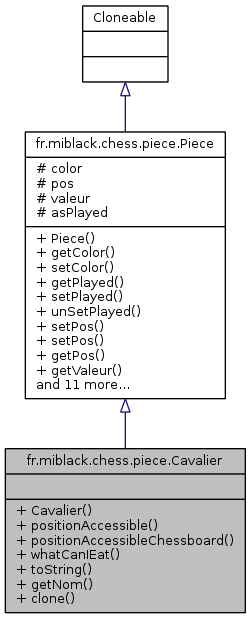
\includegraphics[width=260pt]{classfr_1_1miblack_1_1chess_1_1piece_1_1Cavalier__inherit__graph}
\end{center}
\end{figure}


Collaboration diagram for fr.\-miblack.\-chess.\-piece.\-Cavalier\-:
\nopagebreak
\begin{figure}[H]
\begin{center}
\leavevmode
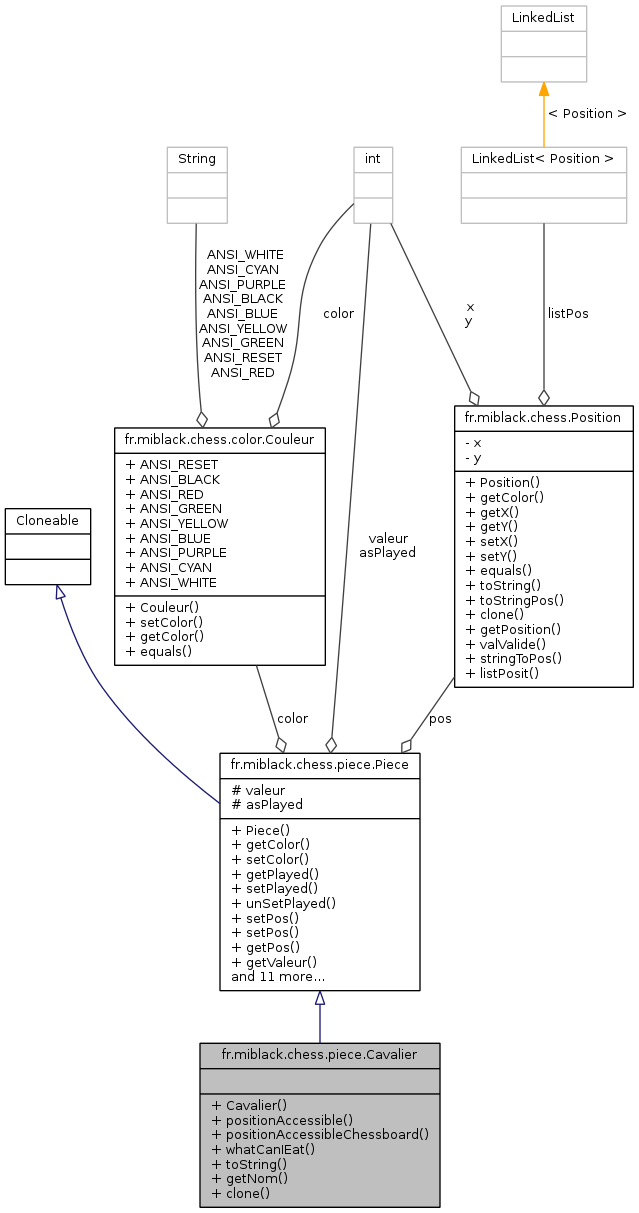
\includegraphics[height=550pt]{classfr_1_1miblack_1_1chess_1_1piece_1_1Cavalier__coll__graph}
\end{center}
\end{figure}
\subsection*{Public Member Functions}
\begin{DoxyCompactItemize}
\item 
{\bf Cavalier} ({\bf Couleur} {\bf color}, {\bf Position} {\bf pos}, int {\bf valeur})
\item 
Linked\-List$<$ {\bf Position} $>$ {\bf position\-Accessible} ()
\item 
Linked\-List$<$ {\bf Position} $>$ {\bf position\-Accessible\-Chessboard} ({\bf Echiquier} chess)
\item 
Linked\-List$<$ {\bf Position} $>$ {\bf what\-Can\-I\-Eat} ({\bf Echiquier} chess)
\item 
String {\bf to\-String} ()
\item 
String {\bf get\-Nom} ()
\item 
{\bf Piece} {\bf clone} ()
\end{DoxyCompactItemize}
\subsection*{Additional Inherited Members}


\subsection{Detailed Description}
\begin{DoxyAuthor}{Author}
mi-\/black 
\end{DoxyAuthor}


\subsection{Constructor \& Destructor Documentation}
\index{fr\-::miblack\-::chess\-::piece\-::\-Cavalier@{fr\-::miblack\-::chess\-::piece\-::\-Cavalier}!Cavalier@{Cavalier}}
\index{Cavalier@{Cavalier}!fr::miblack::chess::piece::Cavalier@{fr\-::miblack\-::chess\-::piece\-::\-Cavalier}}
\subsubsection[{Cavalier}]{\setlength{\rightskip}{0pt plus 5cm}fr.\-miblack.\-chess.\-piece.\-Cavalier.\-Cavalier (
\begin{DoxyParamCaption}
\item[{{\bf Couleur}}]{color, }
\item[{{\bf Position}}]{pos, }
\item[{int}]{valeur}
\end{DoxyParamCaption}
)}\label{classfr_1_1miblack_1_1chess_1_1piece_1_1Cavalier_aa39972e2617dfd572b26ab54ec7e79b5}

\begin{DoxyParams}{Parameters}
{\em color} & \\
\hline
{\em pos} & \\
\hline
{\em valeur} & \\
\hline
\end{DoxyParams}


\subsection{Member Function Documentation}
\index{fr\-::miblack\-::chess\-::piece\-::\-Cavalier@{fr\-::miblack\-::chess\-::piece\-::\-Cavalier}!clone@{clone}}
\index{clone@{clone}!fr::miblack::chess::piece::Cavalier@{fr\-::miblack\-::chess\-::piece\-::\-Cavalier}}
\subsubsection[{clone}]{\setlength{\rightskip}{0pt plus 5cm}{\bf Piece} fr.\-miblack.\-chess.\-piece.\-Cavalier.\-clone (
\begin{DoxyParamCaption}
{}
\end{DoxyParamCaption}
)}\label{classfr_1_1miblack_1_1chess_1_1piece_1_1Cavalier_a8e19cc8f4d445fbc4f2967908a5feefe}
\begin{DoxyReturn}{Returns}

\end{DoxyReturn}
\index{fr\-::miblack\-::chess\-::piece\-::\-Cavalier@{fr\-::miblack\-::chess\-::piece\-::\-Cavalier}!get\-Nom@{get\-Nom}}
\index{get\-Nom@{get\-Nom}!fr::miblack::chess::piece::Cavalier@{fr\-::miblack\-::chess\-::piece\-::\-Cavalier}}
\subsubsection[{get\-Nom}]{\setlength{\rightskip}{0pt plus 5cm}String fr.\-miblack.\-chess.\-piece.\-Cavalier.\-get\-Nom (
\begin{DoxyParamCaption}
{}
\end{DoxyParamCaption}
)}\label{classfr_1_1miblack_1_1chess_1_1piece_1_1Cavalier_a5244f4725912a3b6b6e610d9757a68e0}
\begin{DoxyReturn}{Returns}

\end{DoxyReturn}


Reimplemented from {\bf fr.\-miblack.\-chess.\-piece.\-Piece} \doxyref{}{p.}{classfr_1_1miblack_1_1chess_1_1piece_1_1Piece_a68bb44429e21b7f64511a91a0861dde4}.

\index{fr\-::miblack\-::chess\-::piece\-::\-Cavalier@{fr\-::miblack\-::chess\-::piece\-::\-Cavalier}!position\-Accessible@{position\-Accessible}}
\index{position\-Accessible@{position\-Accessible}!fr::miblack::chess::piece::Cavalier@{fr\-::miblack\-::chess\-::piece\-::\-Cavalier}}
\subsubsection[{position\-Accessible}]{\setlength{\rightskip}{0pt plus 5cm}Linked\-List$<${\bf Position}$>$ fr.\-miblack.\-chess.\-piece.\-Cavalier.\-position\-Accessible (
\begin{DoxyParamCaption}
{}
\end{DoxyParamCaption}
)\hspace{0.3cm}{\ttfamily [virtual]}}\label{classfr_1_1miblack_1_1chess_1_1piece_1_1Cavalier_ab851e7c8f792c86df2d4e1c3f7448428}
\begin{DoxyReturn}{Returns}
List of position where one piece can be going 
\end{DoxyReturn}


Implements {\bf fr.\-miblack.\-chess.\-piece.\-Piece} \doxyref{}{p.}{classfr_1_1miblack_1_1chess_1_1piece_1_1Piece_ad5cdbd635ec706f16d57dccf1b8c456e}.

\index{fr\-::miblack\-::chess\-::piece\-::\-Cavalier@{fr\-::miblack\-::chess\-::piece\-::\-Cavalier}!position\-Accessible\-Chessboard@{position\-Accessible\-Chessboard}}
\index{position\-Accessible\-Chessboard@{position\-Accessible\-Chessboard}!fr::miblack::chess::piece::Cavalier@{fr\-::miblack\-::chess\-::piece\-::\-Cavalier}}
\subsubsection[{position\-Accessible\-Chessboard}]{\setlength{\rightskip}{0pt plus 5cm}Linked\-List$<${\bf Position}$>$ fr.\-miblack.\-chess.\-piece.\-Cavalier.\-position\-Accessible\-Chessboard (
\begin{DoxyParamCaption}
\item[{{\bf Echiquier}}]{chess}
\end{DoxyParamCaption}
)\hspace{0.3cm}{\ttfamily [virtual]}}\label{classfr_1_1miblack_1_1chess_1_1piece_1_1Cavalier_a99eaa1d56a1f687c113116ec12e1ecb4}
\begin{DoxyReturn}{Returns}
List of position where one piece can be going with restriction of the chessboard 
\end{DoxyReturn}


Implements {\bf fr.\-miblack.\-chess.\-piece.\-Piece} \doxyref{}{p.}{classfr_1_1miblack_1_1chess_1_1piece_1_1Piece_ac1222bad9bf13533eecec2b8d99e24c6}.

\index{fr\-::miblack\-::chess\-::piece\-::\-Cavalier@{fr\-::miblack\-::chess\-::piece\-::\-Cavalier}!to\-String@{to\-String}}
\index{to\-String@{to\-String}!fr::miblack::chess::piece::Cavalier@{fr\-::miblack\-::chess\-::piece\-::\-Cavalier}}
\subsubsection[{to\-String}]{\setlength{\rightskip}{0pt plus 5cm}String fr.\-miblack.\-chess.\-piece.\-Cavalier.\-to\-String (
\begin{DoxyParamCaption}
{}
\end{DoxyParamCaption}
)}\label{classfr_1_1miblack_1_1chess_1_1piece_1_1Cavalier_a45104c2f89b14eadc313c27c8c39f45b}
\begin{DoxyReturn}{Returns}

\end{DoxyReturn}
\index{fr\-::miblack\-::chess\-::piece\-::\-Cavalier@{fr\-::miblack\-::chess\-::piece\-::\-Cavalier}!what\-Can\-I\-Eat@{what\-Can\-I\-Eat}}
\index{what\-Can\-I\-Eat@{what\-Can\-I\-Eat}!fr::miblack::chess::piece::Cavalier@{fr\-::miblack\-::chess\-::piece\-::\-Cavalier}}
\subsubsection[{what\-Can\-I\-Eat}]{\setlength{\rightskip}{0pt plus 5cm}Linked\-List$<${\bf Position}$>$ fr.\-miblack.\-chess.\-piece.\-Cavalier.\-what\-Can\-I\-Eat (
\begin{DoxyParamCaption}
\item[{{\bf Echiquier}}]{chess}
\end{DoxyParamCaption}
)\hspace{0.3cm}{\ttfamily [virtual]}}\label{classfr_1_1miblack_1_1chess_1_1piece_1_1Cavalier_ac23e2dfc7769851df8dab0e18ad6d663}

\begin{DoxyParams}{Parameters}
{\em chess} & l'echiquier \\
\hline
\end{DoxyParams}
\begin{DoxyReturn}{Returns}
Liste des position capturables 
\end{DoxyReturn}


Implements {\bf fr.\-miblack.\-chess.\-piece.\-Piece} \doxyref{}{p.}{classfr_1_1miblack_1_1chess_1_1piece_1_1Piece_af18b3bc007e0e50740de39142a5b2919}.



The documentation for this class was generated from the following file\-:\begin{DoxyCompactItemize}
\item 
fr/miblack/chess/piece/{\bf Cavalier.\-java}\end{DoxyCompactItemize}

\section{fr.\-miblack.\-chess.\-color.\-Couleur Class Reference}
\label{classfr_1_1miblack_1_1chess_1_1color_1_1Couleur}\index{fr.\-miblack.\-chess.\-color.\-Couleur@{fr.\-miblack.\-chess.\-color.\-Couleur}}
\subsection*{Public Member Functions}
\begin{DoxyCompactItemize}
\item 
{\bf Couleur} (int {\bf color})
\item 
void {\bf set\-Color} (int {\bf color})
\item 
int {\bf get\-Color} ()
\item 
boolean {\bf equals} ({\bf Couleur} {\bf color})
\end{DoxyCompactItemize}
\subsection*{Static Public Attributes}
\begin{DoxyCompactItemize}
\item 
static final String {\bf A\-N\-S\-I\-\_\-\-R\-E\-S\-E\-T} = \char`\"{}\textbackslash{}u001\-B[0m\char`\"{}
\item 
static final String {\bf A\-N\-S\-I\-\_\-\-B\-L\-A\-C\-K} = \char`\"{}\textbackslash{}u001\-B[30m\char`\"{}
\item 
static final String {\bf A\-N\-S\-I\-\_\-\-R\-E\-D} = \char`\"{}\textbackslash{}u001\-B[31m\char`\"{}
\item 
static final String {\bf A\-N\-S\-I\-\_\-\-G\-R\-E\-E\-N} = \char`\"{}\textbackslash{}u001\-B[32m\char`\"{}
\item 
static final String {\bf A\-N\-S\-I\-\_\-\-Y\-E\-L\-L\-O\-W} = \char`\"{}\textbackslash{}u001\-B[33m\char`\"{}
\item 
static final String {\bf A\-N\-S\-I\-\_\-\-B\-L\-U\-E} = \char`\"{}\textbackslash{}u001\-B[34m\char`\"{}
\item 
static final String {\bf A\-N\-S\-I\-\_\-\-P\-U\-R\-P\-L\-E} = \char`\"{}\textbackslash{}u001\-B[35m\char`\"{}
\item 
static final String {\bf A\-N\-S\-I\-\_\-\-C\-Y\-A\-N} = \char`\"{}\textbackslash{}u001\-B[36m\char`\"{}
\item 
static final String {\bf A\-N\-S\-I\-\_\-\-W\-H\-I\-T\-E} = \char`\"{}\textbackslash{}u001\-B[37m\char`\"{}
\end{DoxyCompactItemize}
\subsection*{Protected Attributes}
\begin{DoxyCompactItemize}
\item 
int {\bf color}
\end{DoxyCompactItemize}


\subsection{Detailed Description}
\begin{DoxyAuthor}{Author}
mi-\/black 
\end{DoxyAuthor}


\subsection{Constructor \& Destructor Documentation}
\index{fr\-::miblack\-::chess\-::color\-::\-Couleur@{fr\-::miblack\-::chess\-::color\-::\-Couleur}!Couleur@{Couleur}}
\index{Couleur@{Couleur}!fr::miblack::chess::color::Couleur@{fr\-::miblack\-::chess\-::color\-::\-Couleur}}
\subsubsection[{Couleur}]{\setlength{\rightskip}{0pt plus 5cm}fr.\-miblack.\-chess.\-color.\-Couleur.\-Couleur (
\begin{DoxyParamCaption}
\item[{int}]{color}
\end{DoxyParamCaption}
)}\label{classfr_1_1miblack_1_1chess_1_1color_1_1Couleur_a417aee90c8fcd9924884dac326cf22e7}

\begin{DoxyParams}{Parameters}
{\em color} & \\
\hline
\end{DoxyParams}


\subsection{Member Function Documentation}
\index{fr\-::miblack\-::chess\-::color\-::\-Couleur@{fr\-::miblack\-::chess\-::color\-::\-Couleur}!equals@{equals}}
\index{equals@{equals}!fr::miblack::chess::color::Couleur@{fr\-::miblack\-::chess\-::color\-::\-Couleur}}
\subsubsection[{equals}]{\setlength{\rightskip}{0pt plus 5cm}boolean fr.\-miblack.\-chess.\-color.\-Couleur.\-equals (
\begin{DoxyParamCaption}
\item[{{\bf Couleur}}]{color}
\end{DoxyParamCaption}
)}\label{classfr_1_1miblack_1_1chess_1_1color_1_1Couleur_aead66043cacc7850c7c84df48ace4275}

\begin{DoxyParams}{Parameters}
{\em color} & \\
\hline
\end{DoxyParams}
\begin{DoxyReturn}{Returns}

\end{DoxyReturn}
\index{fr\-::miblack\-::chess\-::color\-::\-Couleur@{fr\-::miblack\-::chess\-::color\-::\-Couleur}!get\-Color@{get\-Color}}
\index{get\-Color@{get\-Color}!fr::miblack::chess::color::Couleur@{fr\-::miblack\-::chess\-::color\-::\-Couleur}}
\subsubsection[{get\-Color}]{\setlength{\rightskip}{0pt plus 5cm}int fr.\-miblack.\-chess.\-color.\-Couleur.\-get\-Color (
\begin{DoxyParamCaption}
{}
\end{DoxyParamCaption}
)}\label{classfr_1_1miblack_1_1chess_1_1color_1_1Couleur_aa0ff31c3b0c6359a42cc4594bd0d8ccf}
\begin{DoxyReturn}{Returns}

\end{DoxyReturn}
\index{fr\-::miblack\-::chess\-::color\-::\-Couleur@{fr\-::miblack\-::chess\-::color\-::\-Couleur}!set\-Color@{set\-Color}}
\index{set\-Color@{set\-Color}!fr::miblack::chess::color::Couleur@{fr\-::miblack\-::chess\-::color\-::\-Couleur}}
\subsubsection[{set\-Color}]{\setlength{\rightskip}{0pt plus 5cm}void fr.\-miblack.\-chess.\-color.\-Couleur.\-set\-Color (
\begin{DoxyParamCaption}
\item[{int}]{color}
\end{DoxyParamCaption}
)}\label{classfr_1_1miblack_1_1chess_1_1color_1_1Couleur_ab8d13f0a480ec9046d7074695e30580a}

\begin{DoxyParams}{Parameters}
{\em color} & \\
\hline
\end{DoxyParams}


\subsection{Member Data Documentation}
\index{fr\-::miblack\-::chess\-::color\-::\-Couleur@{fr\-::miblack\-::chess\-::color\-::\-Couleur}!A\-N\-S\-I\-\_\-\-B\-L\-A\-C\-K@{A\-N\-S\-I\-\_\-\-B\-L\-A\-C\-K}}
\index{A\-N\-S\-I\-\_\-\-B\-L\-A\-C\-K@{A\-N\-S\-I\-\_\-\-B\-L\-A\-C\-K}!fr::miblack::chess::color::Couleur@{fr\-::miblack\-::chess\-::color\-::\-Couleur}}
\subsubsection[{A\-N\-S\-I\-\_\-\-B\-L\-A\-C\-K}]{\setlength{\rightskip}{0pt plus 5cm}final String fr.\-miblack.\-chess.\-color.\-Couleur.\-A\-N\-S\-I\-\_\-\-B\-L\-A\-C\-K = \char`\"{}\textbackslash{}u001\-B[30m\char`\"{}\hspace{0.3cm}{\ttfamily [static]}}\label{classfr_1_1miblack_1_1chess_1_1color_1_1Couleur_a82be1d7e8d5336d9de8e0a02ec5c407f}
A\-N\-S\-I\-\_\-\-B\-L\-A\-C\-K \index{fr\-::miblack\-::chess\-::color\-::\-Couleur@{fr\-::miblack\-::chess\-::color\-::\-Couleur}!A\-N\-S\-I\-\_\-\-B\-L\-U\-E@{A\-N\-S\-I\-\_\-\-B\-L\-U\-E}}
\index{A\-N\-S\-I\-\_\-\-B\-L\-U\-E@{A\-N\-S\-I\-\_\-\-B\-L\-U\-E}!fr::miblack::chess::color::Couleur@{fr\-::miblack\-::chess\-::color\-::\-Couleur}}
\subsubsection[{A\-N\-S\-I\-\_\-\-B\-L\-U\-E}]{\setlength{\rightskip}{0pt plus 5cm}final String fr.\-miblack.\-chess.\-color.\-Couleur.\-A\-N\-S\-I\-\_\-\-B\-L\-U\-E = \char`\"{}\textbackslash{}u001\-B[34m\char`\"{}\hspace{0.3cm}{\ttfamily [static]}}\label{classfr_1_1miblack_1_1chess_1_1color_1_1Couleur_a5a454183facd609fcc126591b0160979}
A\-N\-S\-I\-\_\-\-B\-L\-U\-E \index{fr\-::miblack\-::chess\-::color\-::\-Couleur@{fr\-::miblack\-::chess\-::color\-::\-Couleur}!A\-N\-S\-I\-\_\-\-C\-Y\-A\-N@{A\-N\-S\-I\-\_\-\-C\-Y\-A\-N}}
\index{A\-N\-S\-I\-\_\-\-C\-Y\-A\-N@{A\-N\-S\-I\-\_\-\-C\-Y\-A\-N}!fr::miblack::chess::color::Couleur@{fr\-::miblack\-::chess\-::color\-::\-Couleur}}
\subsubsection[{A\-N\-S\-I\-\_\-\-C\-Y\-A\-N}]{\setlength{\rightskip}{0pt plus 5cm}final String fr.\-miblack.\-chess.\-color.\-Couleur.\-A\-N\-S\-I\-\_\-\-C\-Y\-A\-N = \char`\"{}\textbackslash{}u001\-B[36m\char`\"{}\hspace{0.3cm}{\ttfamily [static]}}\label{classfr_1_1miblack_1_1chess_1_1color_1_1Couleur_af4c0fcf54c39eb93cdffd66fcf1609c0}
A\-N\-S\-I\-\_\-\-C\-Y\-A\-N \index{fr\-::miblack\-::chess\-::color\-::\-Couleur@{fr\-::miblack\-::chess\-::color\-::\-Couleur}!A\-N\-S\-I\-\_\-\-G\-R\-E\-E\-N@{A\-N\-S\-I\-\_\-\-G\-R\-E\-E\-N}}
\index{A\-N\-S\-I\-\_\-\-G\-R\-E\-E\-N@{A\-N\-S\-I\-\_\-\-G\-R\-E\-E\-N}!fr::miblack::chess::color::Couleur@{fr\-::miblack\-::chess\-::color\-::\-Couleur}}
\subsubsection[{A\-N\-S\-I\-\_\-\-G\-R\-E\-E\-N}]{\setlength{\rightskip}{0pt plus 5cm}final String fr.\-miblack.\-chess.\-color.\-Couleur.\-A\-N\-S\-I\-\_\-\-G\-R\-E\-E\-N = \char`\"{}\textbackslash{}u001\-B[32m\char`\"{}\hspace{0.3cm}{\ttfamily [static]}}\label{classfr_1_1miblack_1_1chess_1_1color_1_1Couleur_a9272b529ae7d50f0adf4a41517f84849}
A\-N\-S\-I\-\_\-\-G\-R\-E\-E\-N \index{fr\-::miblack\-::chess\-::color\-::\-Couleur@{fr\-::miblack\-::chess\-::color\-::\-Couleur}!A\-N\-S\-I\-\_\-\-P\-U\-R\-P\-L\-E@{A\-N\-S\-I\-\_\-\-P\-U\-R\-P\-L\-E}}
\index{A\-N\-S\-I\-\_\-\-P\-U\-R\-P\-L\-E@{A\-N\-S\-I\-\_\-\-P\-U\-R\-P\-L\-E}!fr::miblack::chess::color::Couleur@{fr\-::miblack\-::chess\-::color\-::\-Couleur}}
\subsubsection[{A\-N\-S\-I\-\_\-\-P\-U\-R\-P\-L\-E}]{\setlength{\rightskip}{0pt plus 5cm}final String fr.\-miblack.\-chess.\-color.\-Couleur.\-A\-N\-S\-I\-\_\-\-P\-U\-R\-P\-L\-E = \char`\"{}\textbackslash{}u001\-B[35m\char`\"{}\hspace{0.3cm}{\ttfamily [static]}}\label{classfr_1_1miblack_1_1chess_1_1color_1_1Couleur_ac35d73c1d8bfc3a56ef2ea3766d17833}
A\-N\-S\-I\-\_\-\-P\-U\-R\-P\-L\-E \index{fr\-::miblack\-::chess\-::color\-::\-Couleur@{fr\-::miblack\-::chess\-::color\-::\-Couleur}!A\-N\-S\-I\-\_\-\-R\-E\-D@{A\-N\-S\-I\-\_\-\-R\-E\-D}}
\index{A\-N\-S\-I\-\_\-\-R\-E\-D@{A\-N\-S\-I\-\_\-\-R\-E\-D}!fr::miblack::chess::color::Couleur@{fr\-::miblack\-::chess\-::color\-::\-Couleur}}
\subsubsection[{A\-N\-S\-I\-\_\-\-R\-E\-D}]{\setlength{\rightskip}{0pt plus 5cm}final String fr.\-miblack.\-chess.\-color.\-Couleur.\-A\-N\-S\-I\-\_\-\-R\-E\-D = \char`\"{}\textbackslash{}u001\-B[31m\char`\"{}\hspace{0.3cm}{\ttfamily [static]}}\label{classfr_1_1miblack_1_1chess_1_1color_1_1Couleur_a27eb9a5c9888c69a9493e9ffcb6cc911}
A\-N\-S\-I\-\_\-\-R\-E\-D \index{fr\-::miblack\-::chess\-::color\-::\-Couleur@{fr\-::miblack\-::chess\-::color\-::\-Couleur}!A\-N\-S\-I\-\_\-\-R\-E\-S\-E\-T@{A\-N\-S\-I\-\_\-\-R\-E\-S\-E\-T}}
\index{A\-N\-S\-I\-\_\-\-R\-E\-S\-E\-T@{A\-N\-S\-I\-\_\-\-R\-E\-S\-E\-T}!fr::miblack::chess::color::Couleur@{fr\-::miblack\-::chess\-::color\-::\-Couleur}}
\subsubsection[{A\-N\-S\-I\-\_\-\-R\-E\-S\-E\-T}]{\setlength{\rightskip}{0pt plus 5cm}final String fr.\-miblack.\-chess.\-color.\-Couleur.\-A\-N\-S\-I\-\_\-\-R\-E\-S\-E\-T = \char`\"{}\textbackslash{}u001\-B[0m\char`\"{}\hspace{0.3cm}{\ttfamily [static]}}\label{classfr_1_1miblack_1_1chess_1_1color_1_1Couleur_a519a07c323e0e998ff74f0775c392b76}
A\-N\-S\-I\-\_\-\-R\-E\-S\-E\-T \index{fr\-::miblack\-::chess\-::color\-::\-Couleur@{fr\-::miblack\-::chess\-::color\-::\-Couleur}!A\-N\-S\-I\-\_\-\-W\-H\-I\-T\-E@{A\-N\-S\-I\-\_\-\-W\-H\-I\-T\-E}}
\index{A\-N\-S\-I\-\_\-\-W\-H\-I\-T\-E@{A\-N\-S\-I\-\_\-\-W\-H\-I\-T\-E}!fr::miblack::chess::color::Couleur@{fr\-::miblack\-::chess\-::color\-::\-Couleur}}
\subsubsection[{A\-N\-S\-I\-\_\-\-W\-H\-I\-T\-E}]{\setlength{\rightskip}{0pt plus 5cm}final String fr.\-miblack.\-chess.\-color.\-Couleur.\-A\-N\-S\-I\-\_\-\-W\-H\-I\-T\-E = \char`\"{}\textbackslash{}u001\-B[37m\char`\"{}\hspace{0.3cm}{\ttfamily [static]}}\label{classfr_1_1miblack_1_1chess_1_1color_1_1Couleur_a56f0d3b23c9709b5a2367324e09dcb42}
A\-N\-S\-I\-\_\-\-W\-H\-I\-T\-E \index{fr\-::miblack\-::chess\-::color\-::\-Couleur@{fr\-::miblack\-::chess\-::color\-::\-Couleur}!A\-N\-S\-I\-\_\-\-Y\-E\-L\-L\-O\-W@{A\-N\-S\-I\-\_\-\-Y\-E\-L\-L\-O\-W}}
\index{A\-N\-S\-I\-\_\-\-Y\-E\-L\-L\-O\-W@{A\-N\-S\-I\-\_\-\-Y\-E\-L\-L\-O\-W}!fr::miblack::chess::color::Couleur@{fr\-::miblack\-::chess\-::color\-::\-Couleur}}
\subsubsection[{A\-N\-S\-I\-\_\-\-Y\-E\-L\-L\-O\-W}]{\setlength{\rightskip}{0pt plus 5cm}final String fr.\-miblack.\-chess.\-color.\-Couleur.\-A\-N\-S\-I\-\_\-\-Y\-E\-L\-L\-O\-W = \char`\"{}\textbackslash{}u001\-B[33m\char`\"{}\hspace{0.3cm}{\ttfamily [static]}}\label{classfr_1_1miblack_1_1chess_1_1color_1_1Couleur_abfe59a6c2f5798e2959272ba53212418}
A\-N\-S\-I\-\_\-\-Y\-E\-L\-L\-O\-W \index{fr\-::miblack\-::chess\-::color\-::\-Couleur@{fr\-::miblack\-::chess\-::color\-::\-Couleur}!color@{color}}
\index{color@{color}!fr::miblack::chess::color::Couleur@{fr\-::miblack\-::chess\-::color\-::\-Couleur}}
\subsubsection[{color}]{\setlength{\rightskip}{0pt plus 5cm}int fr.\-miblack.\-chess.\-color.\-Couleur.\-color\hspace{0.3cm}{\ttfamily [protected]}}\label{classfr_1_1miblack_1_1chess_1_1color_1_1Couleur_a51a8fdcfa76057d53b06385515363020}
If sum of line/collon =impaire =$>$ white else black 

The documentation for this class was generated from the following file\-:\begin{DoxyCompactItemize}
\item 
fr/miblack/chess/color/Couleur.\-java\end{DoxyCompactItemize}

\section{fr.\-miblack.\-chess.\-Coup Class Reference}
\label{classfr_1_1miblack_1_1chess_1_1Coup}\index{fr.\-miblack.\-chess.\-Coup@{fr.\-miblack.\-chess.\-Coup}}


Collaboration diagram for fr.\-miblack.\-chess.\-Coup\-:
\nopagebreak
\begin{figure}[H]
\begin{center}
\leavevmode
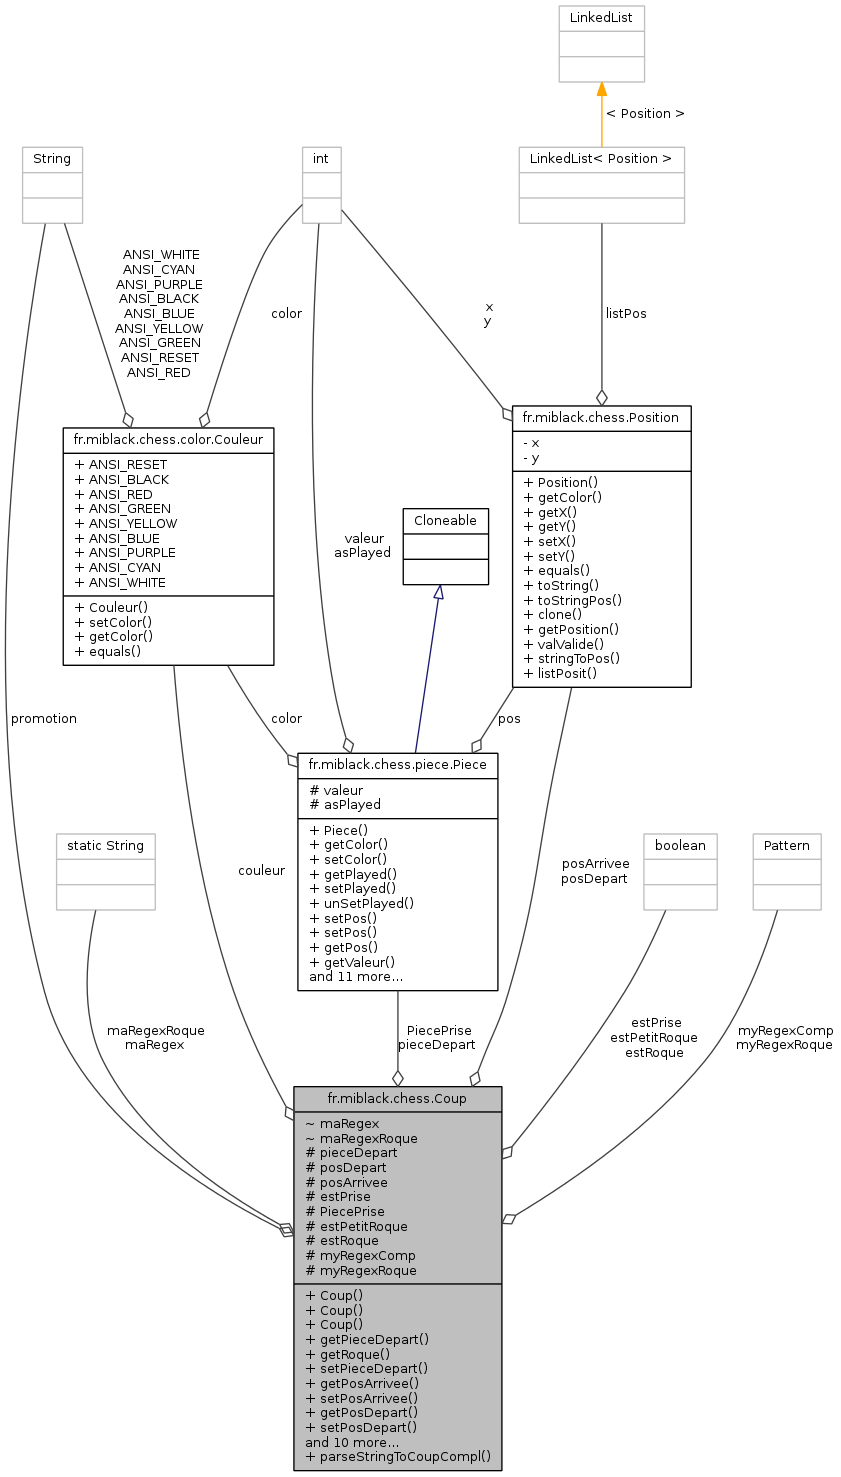
\includegraphics[height=550pt]{classfr_1_1miblack_1_1chess_1_1Coup__coll__graph}
\end{center}
\end{figure}
\subsection*{Public Member Functions}
\begin{DoxyCompactItemize}
\item 
{\bf Coup} (boolean petit\-Roque, {\bf Couleur} {\bf couleur})
\item 
{\bf Coup} ({\bf Piece} {\bf piece\-Depart}, {\bf Position} {\bf pos\-Arrivee}, boolean prise, String {\bf promotion})
\item 
{\bf Coup} ({\bf Piece} {\bf piece\-Depart}, {\bf Position} {\bf pos\-Arrivee}, boolean prise)
\item 
{\bf Piece} {\bf get\-Piece\-Depart} ()
\item 
boolean {\bf get\-Roque} ()
\item 
void {\bf set\-Piece\-Depart} ({\bf Piece} piece)
\item 
{\bf Position} {\bf get\-Pos\-Arrivee} ()
\item 
void {\bf set\-Pos\-Arrivee} ({\bf Position} {\bf pos\-Arrivee})
\item 
{\bf Position} {\bf get\-Pos\-Depart} ()
\item 
void {\bf set\-Pos\-Depart} ({\bf Position} {\bf pos\-Depart})
\item 
String {\bf to\-String} ()
\item 
boolean {\bf is\-Est\-Prise} ()
\item 
void {\bf set\-Est\-Prise} (boolean {\bf est\-Prise})
\item 
boolean {\bf equals} ({\bf Coup} autre)
\item 
{\bf Piece} {\bf get\-Piece\-Prise} ()
\item 
void {\bf set\-Piece\-Prise} ({\bf Piece} piece\-Prise)
\item 
String {\bf get\-Promotion} ()
\item 
void {\bf set\-Promotion} (String {\bf promotion})
\item 
{\bf Couleur} {\bf get\-Couleur} ()
\item 
void {\bf set\-Couleur} ({\bf Couleur} {\bf couleur})
\end{DoxyCompactItemize}
\subsection*{Static Public Member Functions}
\begin{DoxyCompactItemize}
\item 
static {\bf Coup} {\bf parse\-String\-To\-Coup\-Compl} (String my\-String, {\bf Partie} party, {\bf Joueur\-Abstract} p)
\end{DoxyCompactItemize}
\subsection*{Protected Attributes}
\begin{DoxyCompactItemize}
\item 
{\bf Piece} {\bf piece\-Depart}
\item 
{\bf Position} {\bf pos\-Depart}
\item 
{\bf Position} {\bf pos\-Arrivee}
\item 
boolean {\bf est\-Prise}
\item 
{\bf Piece} {\bf Piece\-Prise}
\item 
String {\bf promotion}
\item 
boolean {\bf est\-Petit\-Roque}
\item 
boolean {\bf est\-Roque}
\item 
{\bf Couleur} {\bf couleur}
\end{DoxyCompactItemize}
\subsection*{Static Protected Attributes}
\begin{DoxyCompactItemize}
\item 
static Pattern {\bf my\-Regex\-Comp} = Pattern.\-compile(ma\-Regex )
\item 
static Pattern {\bf my\-Regex\-Roque} = Pattern.\-compile(ma\-Regex\-Roque )
\end{DoxyCompactItemize}


\subsection{Detailed Description}
Cette classe regroupe tout les composant d'un coup \begin{DoxyAuthor}{Author}
mi-\/black 
\end{DoxyAuthor}


\subsection{Constructor \& Destructor Documentation}
\index{fr\-::miblack\-::chess\-::\-Coup@{fr\-::miblack\-::chess\-::\-Coup}!Coup@{Coup}}
\index{Coup@{Coup}!fr::miblack::chess::Coup@{fr\-::miblack\-::chess\-::\-Coup}}
\subsubsection[{Coup}]{\setlength{\rightskip}{0pt plus 5cm}fr.\-miblack.\-chess.\-Coup.\-Coup (
\begin{DoxyParamCaption}
\item[{boolean}]{petit\-Roque, }
\item[{{\bf Couleur}}]{couleur}
\end{DoxyParamCaption}
)}\label{classfr_1_1miblack_1_1chess_1_1Coup_a00f5735ab53a1c5cfbe2c2fd8fa1aa5c}
Constructeur du roque 
\begin{DoxyParams}{Parameters}
{\em petit\-Roque} & \-: un petit roque ? \\
\hline
{\em couleur} & \-: la couleur du roque \\
\hline
\end{DoxyParams}
\index{fr\-::miblack\-::chess\-::\-Coup@{fr\-::miblack\-::chess\-::\-Coup}!Coup@{Coup}}
\index{Coup@{Coup}!fr::miblack::chess::Coup@{fr\-::miblack\-::chess\-::\-Coup}}
\subsubsection[{Coup}]{\setlength{\rightskip}{0pt plus 5cm}fr.\-miblack.\-chess.\-Coup.\-Coup (
\begin{DoxyParamCaption}
\item[{{\bf Piece}}]{piece\-Depart, }
\item[{{\bf Position}}]{pos\-Arrivee, }
\item[{boolean}]{prise, }
\item[{String}]{promotion}
\end{DoxyParamCaption}
)}\label{classfr_1_1miblack_1_1chess_1_1Coup_a24f72a3c1885799b1f23eef11e4883b0}
Constructeur avancé d'un coup , il gère la promotion et la prise 
\begin{DoxyParams}{Parameters}
{\em piece\-Depart} & \\
\hline
{\em pos\-Arrivee} & \\
\hline
{\em prise} & \\
\hline
{\em promotion} & \\
\hline
\end{DoxyParams}
\index{fr\-::miblack\-::chess\-::\-Coup@{fr\-::miblack\-::chess\-::\-Coup}!Coup@{Coup}}
\index{Coup@{Coup}!fr::miblack::chess::Coup@{fr\-::miblack\-::chess\-::\-Coup}}
\subsubsection[{Coup}]{\setlength{\rightskip}{0pt plus 5cm}fr.\-miblack.\-chess.\-Coup.\-Coup (
\begin{DoxyParamCaption}
\item[{{\bf Piece}}]{piece\-Depart, }
\item[{{\bf Position}}]{pos\-Arrivee, }
\item[{boolean}]{prise}
\end{DoxyParamCaption}
)}\label{classfr_1_1miblack_1_1chess_1_1Coup_a63906fa608af2822380bcda5c60f7f69}
Constructeur basique d'un coup avec possibilité de prise 

\subsection{Member Function Documentation}
\index{fr\-::miblack\-::chess\-::\-Coup@{fr\-::miblack\-::chess\-::\-Coup}!equals@{equals}}
\index{equals@{equals}!fr::miblack::chess::Coup@{fr\-::miblack\-::chess\-::\-Coup}}
\subsubsection[{equals}]{\setlength{\rightskip}{0pt plus 5cm}boolean fr.\-miblack.\-chess.\-Coup.\-equals (
\begin{DoxyParamCaption}
\item[{{\bf Coup}}]{autre}
\end{DoxyParamCaption}
)}\label{classfr_1_1miblack_1_1chess_1_1Coup_a7b5790db15bc0ce72eee16fa75ceb948}
test si deux coups sont identiques 
\begin{DoxyParams}{Parameters}
{\em autre} & un autre coup \\
\hline
\end{DoxyParams}
\begin{DoxyReturn}{Returns}
true si equals , false sinon 
\end{DoxyReturn}
\index{fr\-::miblack\-::chess\-::\-Coup@{fr\-::miblack\-::chess\-::\-Coup}!get\-Couleur@{get\-Couleur}}
\index{get\-Couleur@{get\-Couleur}!fr::miblack::chess::Coup@{fr\-::miblack\-::chess\-::\-Coup}}
\subsubsection[{get\-Couleur}]{\setlength{\rightskip}{0pt plus 5cm}{\bf Couleur} fr.\-miblack.\-chess.\-Coup.\-get\-Couleur (
\begin{DoxyParamCaption}
{}
\end{DoxyParamCaption}
)}\label{classfr_1_1miblack_1_1chess_1_1Coup_a3c2f5f8f5628c3863fe067f9bfd6488d}
Get couleur \index{fr\-::miblack\-::chess\-::\-Coup@{fr\-::miblack\-::chess\-::\-Coup}!get\-Piece\-Depart@{get\-Piece\-Depart}}
\index{get\-Piece\-Depart@{get\-Piece\-Depart}!fr::miblack::chess::Coup@{fr\-::miblack\-::chess\-::\-Coup}}
\subsubsection[{get\-Piece\-Depart}]{\setlength{\rightskip}{0pt plus 5cm}{\bf Piece} fr.\-miblack.\-chess.\-Coup.\-get\-Piece\-Depart (
\begin{DoxyParamCaption}
{}
\end{DoxyParamCaption}
)}\label{classfr_1_1miblack_1_1chess_1_1Coup_ac5eec7ef8d5cb16bdc03f3ba19ca3e05}
\begin{DoxyReturn}{Returns}
the piece\-Depart 
\end{DoxyReturn}
\index{fr\-::miblack\-::chess\-::\-Coup@{fr\-::miblack\-::chess\-::\-Coup}!get\-Piece\-Prise@{get\-Piece\-Prise}}
\index{get\-Piece\-Prise@{get\-Piece\-Prise}!fr::miblack::chess::Coup@{fr\-::miblack\-::chess\-::\-Coup}}
\subsubsection[{get\-Piece\-Prise}]{\setlength{\rightskip}{0pt plus 5cm}{\bf Piece} fr.\-miblack.\-chess.\-Coup.\-get\-Piece\-Prise (
\begin{DoxyParamCaption}
{}
\end{DoxyParamCaption}
)}\label{classfr_1_1miblack_1_1chess_1_1Coup_add09eba27d05143dbb08f8c8515c5b00}
La piece prise \begin{DoxyReturn}{Returns}
piece\-Prise 
\end{DoxyReturn}
\index{fr\-::miblack\-::chess\-::\-Coup@{fr\-::miblack\-::chess\-::\-Coup}!get\-Pos\-Arrivee@{get\-Pos\-Arrivee}}
\index{get\-Pos\-Arrivee@{get\-Pos\-Arrivee}!fr::miblack::chess::Coup@{fr\-::miblack\-::chess\-::\-Coup}}
\subsubsection[{get\-Pos\-Arrivee}]{\setlength{\rightskip}{0pt plus 5cm}{\bf Position} fr.\-miblack.\-chess.\-Coup.\-get\-Pos\-Arrivee (
\begin{DoxyParamCaption}
{}
\end{DoxyParamCaption}
)}\label{classfr_1_1miblack_1_1chess_1_1Coup_a4b5dffb465dbd2e62b7b5fd4ad5cd759}
\begin{DoxyReturn}{Returns}
the pos\-Arrivee 
\end{DoxyReturn}
\index{fr\-::miblack\-::chess\-::\-Coup@{fr\-::miblack\-::chess\-::\-Coup}!get\-Pos\-Depart@{get\-Pos\-Depart}}
\index{get\-Pos\-Depart@{get\-Pos\-Depart}!fr::miblack::chess::Coup@{fr\-::miblack\-::chess\-::\-Coup}}
\subsubsection[{get\-Pos\-Depart}]{\setlength{\rightskip}{0pt plus 5cm}{\bf Position} fr.\-miblack.\-chess.\-Coup.\-get\-Pos\-Depart (
\begin{DoxyParamCaption}
{}
\end{DoxyParamCaption}
)}\label{classfr_1_1miblack_1_1chess_1_1Coup_a1bf41dc5a891d29c4e63b356f4bf083d}
\begin{DoxyReturn}{Returns}
the pos\-Depart 
\end{DoxyReturn}
\index{fr\-::miblack\-::chess\-::\-Coup@{fr\-::miblack\-::chess\-::\-Coup}!get\-Promotion@{get\-Promotion}}
\index{get\-Promotion@{get\-Promotion}!fr::miblack::chess::Coup@{fr\-::miblack\-::chess\-::\-Coup}}
\subsubsection[{get\-Promotion}]{\setlength{\rightskip}{0pt plus 5cm}String fr.\-miblack.\-chess.\-Coup.\-get\-Promotion (
\begin{DoxyParamCaption}
{}
\end{DoxyParamCaption}
)}\label{classfr_1_1miblack_1_1chess_1_1Coup_ac910339a2a1dda344c0984ce4f11b5db}
get Promotion \index{fr\-::miblack\-::chess\-::\-Coup@{fr\-::miblack\-::chess\-::\-Coup}!get\-Roque@{get\-Roque}}
\index{get\-Roque@{get\-Roque}!fr::miblack::chess::Coup@{fr\-::miblack\-::chess\-::\-Coup}}
\subsubsection[{get\-Roque}]{\setlength{\rightskip}{0pt plus 5cm}boolean fr.\-miblack.\-chess.\-Coup.\-get\-Roque (
\begin{DoxyParamCaption}
{}
\end{DoxyParamCaption}
)}\label{classfr_1_1miblack_1_1chess_1_1Coup_a90b23bb7a59c2a9ff2e2192b73992df2}
Recupère si le coup est un roque \begin{DoxyReturn}{Returns}
est\-Roque ? 
\end{DoxyReturn}
\index{fr\-::miblack\-::chess\-::\-Coup@{fr\-::miblack\-::chess\-::\-Coup}!is\-Est\-Prise@{is\-Est\-Prise}}
\index{is\-Est\-Prise@{is\-Est\-Prise}!fr::miblack::chess::Coup@{fr\-::miblack\-::chess\-::\-Coup}}
\subsubsection[{is\-Est\-Prise}]{\setlength{\rightskip}{0pt plus 5cm}boolean fr.\-miblack.\-chess.\-Coup.\-is\-Est\-Prise (
\begin{DoxyParamCaption}
{}
\end{DoxyParamCaption}
)}\label{classfr_1_1miblack_1_1chess_1_1Coup_acf1ee7ece76d7b9680d7a4b9523b45a3}
Le coup est une prise ? \begin{DoxyReturn}{Returns}
est\-Prise 
\end{DoxyReturn}
\index{fr\-::miblack\-::chess\-::\-Coup@{fr\-::miblack\-::chess\-::\-Coup}!parse\-String\-To\-Coup\-Compl@{parse\-String\-To\-Coup\-Compl}}
\index{parse\-String\-To\-Coup\-Compl@{parse\-String\-To\-Coup\-Compl}!fr::miblack::chess::Coup@{fr\-::miblack\-::chess\-::\-Coup}}
\subsubsection[{parse\-String\-To\-Coup\-Compl}]{\setlength{\rightskip}{0pt plus 5cm}static {\bf Coup} fr.\-miblack.\-chess.\-Coup.\-parse\-String\-To\-Coup\-Compl (
\begin{DoxyParamCaption}
\item[{String}]{my\-String, }
\item[{{\bf Partie}}]{party, }
\item[{{\bf Joueur\-Abstract}}]{p}
\end{DoxyParamCaption}
)\hspace{0.3cm}{\ttfamily [static]}}\label{classfr_1_1miblack_1_1chess_1_1Coup_a6af53f0364768d4257ce99a2823d3aa8}

\begin{DoxyParams}{Parameters}
{\em my\-String} & chaine style a2-\/a4 \\
\hline
{\em party} & la partie \\
\hline
{\em p} & le joueur \\
\hline
\end{DoxyParams}
\begin{DoxyReturn}{Returns}
a new \doxyref{Coup}{p.}{classfr_1_1miblack_1_1chess_1_1Coup} avec tout comme il faut ! 
\end{DoxyReturn}
\index{fr\-::miblack\-::chess\-::\-Coup@{fr\-::miblack\-::chess\-::\-Coup}!set\-Couleur@{set\-Couleur}}
\index{set\-Couleur@{set\-Couleur}!fr::miblack::chess::Coup@{fr\-::miblack\-::chess\-::\-Coup}}
\subsubsection[{set\-Couleur}]{\setlength{\rightskip}{0pt plus 5cm}void fr.\-miblack.\-chess.\-Coup.\-set\-Couleur (
\begin{DoxyParamCaption}
\item[{{\bf Couleur}}]{couleur}
\end{DoxyParamCaption}
)}\label{classfr_1_1miblack_1_1chess_1_1Coup_a80431ab5e72e4f5e42a0762baa83867c}
Set couleur \index{fr\-::miblack\-::chess\-::\-Coup@{fr\-::miblack\-::chess\-::\-Coup}!set\-Est\-Prise@{set\-Est\-Prise}}
\index{set\-Est\-Prise@{set\-Est\-Prise}!fr::miblack::chess::Coup@{fr\-::miblack\-::chess\-::\-Coup}}
\subsubsection[{set\-Est\-Prise}]{\setlength{\rightskip}{0pt plus 5cm}void fr.\-miblack.\-chess.\-Coup.\-set\-Est\-Prise (
\begin{DoxyParamCaption}
\item[{boolean}]{est\-Prise}
\end{DoxyParamCaption}
)}\label{classfr_1_1miblack_1_1chess_1_1Coup_a8559cedf5e035ac73ecea420ab43b1a6}
Set est\-Prise \index{fr\-::miblack\-::chess\-::\-Coup@{fr\-::miblack\-::chess\-::\-Coup}!set\-Piece\-Depart@{set\-Piece\-Depart}}
\index{set\-Piece\-Depart@{set\-Piece\-Depart}!fr::miblack::chess::Coup@{fr\-::miblack\-::chess\-::\-Coup}}
\subsubsection[{set\-Piece\-Depart}]{\setlength{\rightskip}{0pt plus 5cm}void fr.\-miblack.\-chess.\-Coup.\-set\-Piece\-Depart (
\begin{DoxyParamCaption}
\item[{{\bf Piece}}]{piece}
\end{DoxyParamCaption}
)}\label{classfr_1_1miblack_1_1chess_1_1Coup_aab00cf8d6476a51d81565de4f3b1c516}
the piece\-Depart to set 
\begin{DoxyParams}{Parameters}
{\em piece} & \\
\hline
\end{DoxyParams}
\index{fr\-::miblack\-::chess\-::\-Coup@{fr\-::miblack\-::chess\-::\-Coup}!set\-Piece\-Prise@{set\-Piece\-Prise}}
\index{set\-Piece\-Prise@{set\-Piece\-Prise}!fr::miblack::chess::Coup@{fr\-::miblack\-::chess\-::\-Coup}}
\subsubsection[{set\-Piece\-Prise}]{\setlength{\rightskip}{0pt plus 5cm}void fr.\-miblack.\-chess.\-Coup.\-set\-Piece\-Prise (
\begin{DoxyParamCaption}
\item[{{\bf Piece}}]{piece\-Prise}
\end{DoxyParamCaption}
)}\label{classfr_1_1miblack_1_1chess_1_1Coup_a04e74b029f082393339b9703aee97c80}
Set piece\-Prise \index{fr\-::miblack\-::chess\-::\-Coup@{fr\-::miblack\-::chess\-::\-Coup}!set\-Pos\-Arrivee@{set\-Pos\-Arrivee}}
\index{set\-Pos\-Arrivee@{set\-Pos\-Arrivee}!fr::miblack::chess::Coup@{fr\-::miblack\-::chess\-::\-Coup}}
\subsubsection[{set\-Pos\-Arrivee}]{\setlength{\rightskip}{0pt plus 5cm}void fr.\-miblack.\-chess.\-Coup.\-set\-Pos\-Arrivee (
\begin{DoxyParamCaption}
\item[{{\bf Position}}]{pos\-Arrivee}
\end{DoxyParamCaption}
)}\label{classfr_1_1miblack_1_1chess_1_1Coup_a8345a2624f08a45540eade3912505dde}

\begin{DoxyParams}{Parameters}
{\em pos\-Arrivee} & the pos\-Arrivee to set \\
\hline
\end{DoxyParams}
\index{fr\-::miblack\-::chess\-::\-Coup@{fr\-::miblack\-::chess\-::\-Coup}!set\-Pos\-Depart@{set\-Pos\-Depart}}
\index{set\-Pos\-Depart@{set\-Pos\-Depart}!fr::miblack::chess::Coup@{fr\-::miblack\-::chess\-::\-Coup}}
\subsubsection[{set\-Pos\-Depart}]{\setlength{\rightskip}{0pt plus 5cm}void fr.\-miblack.\-chess.\-Coup.\-set\-Pos\-Depart (
\begin{DoxyParamCaption}
\item[{{\bf Position}}]{pos\-Depart}
\end{DoxyParamCaption}
)}\label{classfr_1_1miblack_1_1chess_1_1Coup_afed52ebdb1055716abba92967817f3c4}

\begin{DoxyParams}{Parameters}
{\em pos\-Depart} & the pos\-Depart to set \\
\hline
\end{DoxyParams}
\index{fr\-::miblack\-::chess\-::\-Coup@{fr\-::miblack\-::chess\-::\-Coup}!set\-Promotion@{set\-Promotion}}
\index{set\-Promotion@{set\-Promotion}!fr::miblack::chess::Coup@{fr\-::miblack\-::chess\-::\-Coup}}
\subsubsection[{set\-Promotion}]{\setlength{\rightskip}{0pt plus 5cm}void fr.\-miblack.\-chess.\-Coup.\-set\-Promotion (
\begin{DoxyParamCaption}
\item[{String}]{promotion}
\end{DoxyParamCaption}
)}\label{classfr_1_1miblack_1_1chess_1_1Coup_a63bfcdc470ab1352cd717b3c87b7b315}
Set promotion \index{fr\-::miblack\-::chess\-::\-Coup@{fr\-::miblack\-::chess\-::\-Coup}!to\-String@{to\-String}}
\index{to\-String@{to\-String}!fr::miblack::chess::Coup@{fr\-::miblack\-::chess\-::\-Coup}}
\subsubsection[{to\-String}]{\setlength{\rightskip}{0pt plus 5cm}String fr.\-miblack.\-chess.\-Coup.\-to\-String (
\begin{DoxyParamCaption}
{}
\end{DoxyParamCaption}
)}\label{classfr_1_1miblack_1_1chess_1_1Coup_a5ada925c6b985565c262c6306f6fc15b}
\begin{DoxyReturn}{Returns}
La chaine d'un coup , lisible par un homme 
\end{DoxyReturn}


\subsection{Member Data Documentation}
\index{fr\-::miblack\-::chess\-::\-Coup@{fr\-::miblack\-::chess\-::\-Coup}!couleur@{couleur}}
\index{couleur@{couleur}!fr::miblack::chess::Coup@{fr\-::miblack\-::chess\-::\-Coup}}
\subsubsection[{couleur}]{\setlength{\rightskip}{0pt plus 5cm}{\bf Couleur} fr.\-miblack.\-chess.\-Coup.\-couleur\hspace{0.3cm}{\ttfamily [protected]}}\label{classfr_1_1miblack_1_1chess_1_1Coup_a62a11c9776a1ee250ca8e1f45a0e58a4}
Couleur du coup (utile pour le roque) \index{fr\-::miblack\-::chess\-::\-Coup@{fr\-::miblack\-::chess\-::\-Coup}!est\-Petit\-Roque@{est\-Petit\-Roque}}
\index{est\-Petit\-Roque@{est\-Petit\-Roque}!fr::miblack::chess::Coup@{fr\-::miblack\-::chess\-::\-Coup}}
\subsubsection[{est\-Petit\-Roque}]{\setlength{\rightskip}{0pt plus 5cm}boolean fr.\-miblack.\-chess.\-Coup.\-est\-Petit\-Roque\hspace{0.3cm}{\ttfamily [protected]}}\label{classfr_1_1miblack_1_1chess_1_1Coup_a7614a983d830ba2675b18c7a04340585}
Le coup est un petit roque ? \index{fr\-::miblack\-::chess\-::\-Coup@{fr\-::miblack\-::chess\-::\-Coup}!est\-Prise@{est\-Prise}}
\index{est\-Prise@{est\-Prise}!fr::miblack::chess::Coup@{fr\-::miblack\-::chess\-::\-Coup}}
\subsubsection[{est\-Prise}]{\setlength{\rightskip}{0pt plus 5cm}boolean fr.\-miblack.\-chess.\-Coup.\-est\-Prise\hspace{0.3cm}{\ttfamily [protected]}}\label{classfr_1_1miblack_1_1chess_1_1Coup_a76aff266a2adb99c21c23a85457c77a8}
Le coup est une prise ? \index{fr\-::miblack\-::chess\-::\-Coup@{fr\-::miblack\-::chess\-::\-Coup}!est\-Roque@{est\-Roque}}
\index{est\-Roque@{est\-Roque}!fr::miblack::chess::Coup@{fr\-::miblack\-::chess\-::\-Coup}}
\subsubsection[{est\-Roque}]{\setlength{\rightskip}{0pt plus 5cm}boolean fr.\-miblack.\-chess.\-Coup.\-est\-Roque\hspace{0.3cm}{\ttfamily [protected]}}\label{classfr_1_1miblack_1_1chess_1_1Coup_a1a2abd0994de4a0ffb0c1d302b75a4d9}
Le coup est un roque ? \index{fr\-::miblack\-::chess\-::\-Coup@{fr\-::miblack\-::chess\-::\-Coup}!my\-Regex\-Comp@{my\-Regex\-Comp}}
\index{my\-Regex\-Comp@{my\-Regex\-Comp}!fr::miblack::chess::Coup@{fr\-::miblack\-::chess\-::\-Coup}}
\subsubsection[{my\-Regex\-Comp}]{\setlength{\rightskip}{0pt plus 5cm}Pattern fr.\-miblack.\-chess.\-Coup.\-my\-Regex\-Comp = Pattern.\-compile(ma\-Regex )\hspace{0.3cm}{\ttfamily [static]}, {\ttfamily [protected]}}\label{classfr_1_1miblack_1_1chess_1_1Coup_a55308b644c3853fbaf21f0bb77ac6e5f}
my\-Regex\-Comp est un parttern (une sorte de moule) ou l'on insère une regex ici ma\-Regex \index{fr\-::miblack\-::chess\-::\-Coup@{fr\-::miblack\-::chess\-::\-Coup}!my\-Regex\-Roque@{my\-Regex\-Roque}}
\index{my\-Regex\-Roque@{my\-Regex\-Roque}!fr::miblack::chess::Coup@{fr\-::miblack\-::chess\-::\-Coup}}
\subsubsection[{my\-Regex\-Roque}]{\setlength{\rightskip}{0pt plus 5cm}Pattern fr.\-miblack.\-chess.\-Coup.\-my\-Regex\-Roque = Pattern.\-compile(ma\-Regex\-Roque )\hspace{0.3cm}{\ttfamily [static]}, {\ttfamily [protected]}}\label{classfr_1_1miblack_1_1chess_1_1Coup_ac50c3d7aae292fcd6fdfcb50f96bc157}
my\-Regex\-Roque est un parttern (une sorte de moule) ou l'on insère une regex ici ma\-Regex\-Roque \index{fr\-::miblack\-::chess\-::\-Coup@{fr\-::miblack\-::chess\-::\-Coup}!piece\-Depart@{piece\-Depart}}
\index{piece\-Depart@{piece\-Depart}!fr::miblack::chess::Coup@{fr\-::miblack\-::chess\-::\-Coup}}
\subsubsection[{piece\-Depart}]{\setlength{\rightskip}{0pt plus 5cm}{\bf Piece} fr.\-miblack.\-chess.\-Coup.\-piece\-Depart\hspace{0.3cm}{\ttfamily [protected]}}\label{classfr_1_1miblack_1_1chess_1_1Coup_a6cd0a6e47db2d9c1125cd70f1e8d394a}
La piece d'ou part le coup \index{fr\-::miblack\-::chess\-::\-Coup@{fr\-::miblack\-::chess\-::\-Coup}!Piece\-Prise@{Piece\-Prise}}
\index{Piece\-Prise@{Piece\-Prise}!fr::miblack::chess::Coup@{fr\-::miblack\-::chess\-::\-Coup}}
\subsubsection[{Piece\-Prise}]{\setlength{\rightskip}{0pt plus 5cm}{\bf Piece} fr.\-miblack.\-chess.\-Coup.\-Piece\-Prise\hspace{0.3cm}{\ttfamily [protected]}}\label{classfr_1_1miblack_1_1chess_1_1Coup_a846bbb5d09b53001148e39e443358ca9}
Dans le cas d'une prise , on stock la piece \index{fr\-::miblack\-::chess\-::\-Coup@{fr\-::miblack\-::chess\-::\-Coup}!pos\-Arrivee@{pos\-Arrivee}}
\index{pos\-Arrivee@{pos\-Arrivee}!fr::miblack::chess::Coup@{fr\-::miblack\-::chess\-::\-Coup}}
\subsubsection[{pos\-Arrivee}]{\setlength{\rightskip}{0pt plus 5cm}{\bf Position} fr.\-miblack.\-chess.\-Coup.\-pos\-Arrivee\hspace{0.3cm}{\ttfamily [protected]}}\label{classfr_1_1miblack_1_1chess_1_1Coup_adf9f70424784a558e9582d91f526a3cd}
La position d'arrivée du coup \index{fr\-::miblack\-::chess\-::\-Coup@{fr\-::miblack\-::chess\-::\-Coup}!pos\-Depart@{pos\-Depart}}
\index{pos\-Depart@{pos\-Depart}!fr::miblack::chess::Coup@{fr\-::miblack\-::chess\-::\-Coup}}
\subsubsection[{pos\-Depart}]{\setlength{\rightskip}{0pt plus 5cm}{\bf Position} fr.\-miblack.\-chess.\-Coup.\-pos\-Depart\hspace{0.3cm}{\ttfamily [protected]}}\label{classfr_1_1miblack_1_1chess_1_1Coup_a24e0328382f4de4df49b55b365ab4845}
La position d'ou part le coup \index{fr\-::miblack\-::chess\-::\-Coup@{fr\-::miblack\-::chess\-::\-Coup}!promotion@{promotion}}
\index{promotion@{promotion}!fr::miblack::chess::Coup@{fr\-::miblack\-::chess\-::\-Coup}}
\subsubsection[{promotion}]{\setlength{\rightskip}{0pt plus 5cm}String fr.\-miblack.\-chess.\-Coup.\-promotion\hspace{0.3cm}{\ttfamily [protected]}}\label{classfr_1_1miblack_1_1chess_1_1Coup_ab585ab255d91ee9defc16b4d2a082f0f}
En quoi la piece est promus D F T ou C 

The documentation for this class was generated from the following file\-:\begin{DoxyCompactItemize}
\item 
fr/miblack/chess/{\bf Coup.\-java}\end{DoxyCompactItemize}

\section{fr.\-miblack.\-chess.\-piece.\-Dame Class Reference}
\label{classfr_1_1miblack_1_1chess_1_1piece_1_1Dame}\index{fr.\-miblack.\-chess.\-piece.\-Dame@{fr.\-miblack.\-chess.\-piece.\-Dame}}
Inheritance diagram for fr.\-miblack.\-chess.\-piece.\-Dame\-:\begin{figure}[H]
\begin{center}
\leavevmode
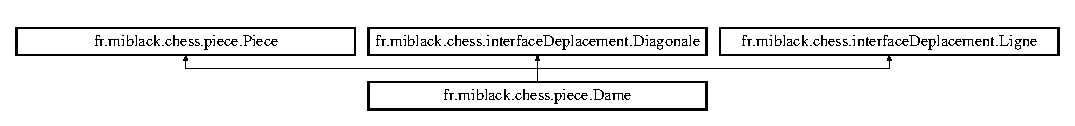
\includegraphics[height=1.244444cm]{classfr_1_1miblack_1_1chess_1_1piece_1_1Dame}
\end{center}
\end{figure}
\subsection*{Public Member Functions}
\begin{DoxyCompactItemize}
\item 
{\bf Dame} ({\bf Couleur} {\bf color}, {\bf Position} {\bf pos}, int {\bf valeur})
\item 
Linked\-List$<$ {\bf Position} $>$ {\bf position\-Accessible} ()
\item 
Linked\-List$<$ {\bf Position} $>$ {\bf position\-Accessible\-Chessboard} ({\bf Echiquier} chess)
\item 
Linked\-List$<$ {\bf Position} $>$ {\bf what\-Can\-I\-Eat} ({\bf Echiquier} chess)
\item 
Linked\-List$<$ {\bf Position} $>$ {\bf position\-Diagonale} ()
\item 
Linked\-List$<$ {\bf Position} $>$ {\bf position\-Ligne} ()
\item 
String {\bf to\-String} ()
\item 
String {\bf get\-Nom} ()
\item 
{\bf Piece} {\bf clone} ()
\end{DoxyCompactItemize}
\subsection*{Additional Inherited Members}


\subsection{Detailed Description}
\begin{DoxyAuthor}{Author}
mi-\/black 
\end{DoxyAuthor}


\subsection{Constructor \& Destructor Documentation}
\index{fr\-::miblack\-::chess\-::piece\-::\-Dame@{fr\-::miblack\-::chess\-::piece\-::\-Dame}!Dame@{Dame}}
\index{Dame@{Dame}!fr::miblack::chess::piece::Dame@{fr\-::miblack\-::chess\-::piece\-::\-Dame}}
\subsubsection[{Dame}]{\setlength{\rightskip}{0pt plus 5cm}fr.\-miblack.\-chess.\-piece.\-Dame.\-Dame (
\begin{DoxyParamCaption}
\item[{{\bf Couleur}}]{color, }
\item[{{\bf Position}}]{pos, }
\item[{int}]{valeur}
\end{DoxyParamCaption}
)}\label{classfr_1_1miblack_1_1chess_1_1piece_1_1Dame_aecf6e01428e37f4e3ffd2c327016e36c}

\begin{DoxyParams}{Parameters}
{\em color} & \\
\hline
{\em pos} & \\
\hline
{\em valeur} & \\
\hline
\end{DoxyParams}


\subsection{Member Function Documentation}
\index{fr\-::miblack\-::chess\-::piece\-::\-Dame@{fr\-::miblack\-::chess\-::piece\-::\-Dame}!clone@{clone}}
\index{clone@{clone}!fr::miblack::chess::piece::Dame@{fr\-::miblack\-::chess\-::piece\-::\-Dame}}
\subsubsection[{clone}]{\setlength{\rightskip}{0pt plus 5cm}{\bf Piece} fr.\-miblack.\-chess.\-piece.\-Dame.\-clone (
\begin{DoxyParamCaption}
{}
\end{DoxyParamCaption}
)}\label{classfr_1_1miblack_1_1chess_1_1piece_1_1Dame_ade5ba6a58cbd2b69db81155c46a023ab}
\begin{DoxyReturn}{Returns}

\end{DoxyReturn}
\index{fr\-::miblack\-::chess\-::piece\-::\-Dame@{fr\-::miblack\-::chess\-::piece\-::\-Dame}!get\-Nom@{get\-Nom}}
\index{get\-Nom@{get\-Nom}!fr::miblack::chess::piece::Dame@{fr\-::miblack\-::chess\-::piece\-::\-Dame}}
\subsubsection[{get\-Nom}]{\setlength{\rightskip}{0pt plus 5cm}String fr.\-miblack.\-chess.\-piece.\-Dame.\-get\-Nom (
\begin{DoxyParamCaption}
{}
\end{DoxyParamCaption}
)}\label{classfr_1_1miblack_1_1chess_1_1piece_1_1Dame_a4d16e6c8afc12ee3962905947f4fba00}
\begin{DoxyReturn}{Returns}

\end{DoxyReturn}


Reimplemented from {\bf fr.\-miblack.\-chess.\-piece.\-Piece} \doxyref{}{p.}{classfr_1_1miblack_1_1chess_1_1piece_1_1Piece_a68bb44429e21b7f64511a91a0861dde4}.

\index{fr\-::miblack\-::chess\-::piece\-::\-Dame@{fr\-::miblack\-::chess\-::piece\-::\-Dame}!position\-Accessible@{position\-Accessible}}
\index{position\-Accessible@{position\-Accessible}!fr::miblack::chess::piece::Dame@{fr\-::miblack\-::chess\-::piece\-::\-Dame}}
\subsubsection[{position\-Accessible}]{\setlength{\rightskip}{0pt plus 5cm}Linked\-List$<${\bf Position}$>$ fr.\-miblack.\-chess.\-piece.\-Dame.\-position\-Accessible (
\begin{DoxyParamCaption}
{}
\end{DoxyParamCaption}
)\hspace{0.3cm}{\ttfamily [virtual]}}\label{classfr_1_1miblack_1_1chess_1_1piece_1_1Dame_ac25901344ee4e07425d9e3704cd22802}
\begin{DoxyReturn}{Returns}
List of position where one piece can be going 
\end{DoxyReturn}


Implements {\bf fr.\-miblack.\-chess.\-piece.\-Piece} \doxyref{}{p.}{classfr_1_1miblack_1_1chess_1_1piece_1_1Piece_ad5cdbd635ec706f16d57dccf1b8c456e}.

\index{fr\-::miblack\-::chess\-::piece\-::\-Dame@{fr\-::miblack\-::chess\-::piece\-::\-Dame}!position\-Accessible\-Chessboard@{position\-Accessible\-Chessboard}}
\index{position\-Accessible\-Chessboard@{position\-Accessible\-Chessboard}!fr::miblack::chess::piece::Dame@{fr\-::miblack\-::chess\-::piece\-::\-Dame}}
\subsubsection[{position\-Accessible\-Chessboard}]{\setlength{\rightskip}{0pt plus 5cm}Linked\-List$<${\bf Position}$>$ fr.\-miblack.\-chess.\-piece.\-Dame.\-position\-Accessible\-Chessboard (
\begin{DoxyParamCaption}
\item[{{\bf Echiquier}}]{chess}
\end{DoxyParamCaption}
)\hspace{0.3cm}{\ttfamily [virtual]}}\label{classfr_1_1miblack_1_1chess_1_1piece_1_1Dame_a9b0273eab6398694c36cd5a52d985801}
\begin{DoxyReturn}{Returns}
List of position where one piece can be going with restriction of the chessboard 
\end{DoxyReturn}


Implements {\bf fr.\-miblack.\-chess.\-piece.\-Piece} \doxyref{}{p.}{classfr_1_1miblack_1_1chess_1_1piece_1_1Piece_ac1222bad9bf13533eecec2b8d99e24c6}.

\index{fr\-::miblack\-::chess\-::piece\-::\-Dame@{fr\-::miblack\-::chess\-::piece\-::\-Dame}!position\-Diagonale@{position\-Diagonale}}
\index{position\-Diagonale@{position\-Diagonale}!fr::miblack::chess::piece::Dame@{fr\-::miblack\-::chess\-::piece\-::\-Dame}}
\subsubsection[{position\-Diagonale}]{\setlength{\rightskip}{0pt plus 5cm}Linked\-List$<${\bf Position}$>$ fr.\-miblack.\-chess.\-piece.\-Dame.\-position\-Diagonale (
\begin{DoxyParamCaption}
{}
\end{DoxyParamCaption}
)}\label{classfr_1_1miblack_1_1chess_1_1piece_1_1Dame_a6e03b316c8e420a3fab05f2afae4c677}
\begin{DoxyReturn}{Returns}
liste des pos diagonales 
\end{DoxyReturn}


Implements {\bf fr.\-miblack.\-chess.\-interface\-Deplacement.\-Diagonale} \doxyref{}{p.}{interfacefr_1_1miblack_1_1chess_1_1interfaceDeplacement_1_1Diagonale_a4d6e3ca777cea05ea561875497ac1161}.

\index{fr\-::miblack\-::chess\-::piece\-::\-Dame@{fr\-::miblack\-::chess\-::piece\-::\-Dame}!position\-Ligne@{position\-Ligne}}
\index{position\-Ligne@{position\-Ligne}!fr::miblack::chess::piece::Dame@{fr\-::miblack\-::chess\-::piece\-::\-Dame}}
\subsubsection[{position\-Ligne}]{\setlength{\rightskip}{0pt plus 5cm}Linked\-List$<${\bf Position}$>$ fr.\-miblack.\-chess.\-piece.\-Dame.\-position\-Ligne (
\begin{DoxyParamCaption}
{}
\end{DoxyParamCaption}
)}\label{classfr_1_1miblack_1_1chess_1_1piece_1_1Dame_a4d2aaeb188e82f1f801e5c8311677362}
\begin{DoxyReturn}{Returns}
liste des pos en ligne 
\end{DoxyReturn}


Implements {\bf fr.\-miblack.\-chess.\-interface\-Deplacement.\-Ligne} \doxyref{}{p.}{interfacefr_1_1miblack_1_1chess_1_1interfaceDeplacement_1_1Ligne_a55b5c0cdf05915b5996754c845591399}.

\index{fr\-::miblack\-::chess\-::piece\-::\-Dame@{fr\-::miblack\-::chess\-::piece\-::\-Dame}!to\-String@{to\-String}}
\index{to\-String@{to\-String}!fr::miblack::chess::piece::Dame@{fr\-::miblack\-::chess\-::piece\-::\-Dame}}
\subsubsection[{to\-String}]{\setlength{\rightskip}{0pt plus 5cm}String fr.\-miblack.\-chess.\-piece.\-Dame.\-to\-String (
\begin{DoxyParamCaption}
{}
\end{DoxyParamCaption}
)}\label{classfr_1_1miblack_1_1chess_1_1piece_1_1Dame_ad0a93b9c8602c677d9026f91a4c15243}
\begin{DoxyReturn}{Returns}

\end{DoxyReturn}
\index{fr\-::miblack\-::chess\-::piece\-::\-Dame@{fr\-::miblack\-::chess\-::piece\-::\-Dame}!what\-Can\-I\-Eat@{what\-Can\-I\-Eat}}
\index{what\-Can\-I\-Eat@{what\-Can\-I\-Eat}!fr::miblack::chess::piece::Dame@{fr\-::miblack\-::chess\-::piece\-::\-Dame}}
\subsubsection[{what\-Can\-I\-Eat}]{\setlength{\rightskip}{0pt plus 5cm}Linked\-List$<${\bf Position}$>$ fr.\-miblack.\-chess.\-piece.\-Dame.\-what\-Can\-I\-Eat (
\begin{DoxyParamCaption}
\item[{{\bf Echiquier}}]{chess}
\end{DoxyParamCaption}
)\hspace{0.3cm}{\ttfamily [virtual]}}\label{classfr_1_1miblack_1_1chess_1_1piece_1_1Dame_a1220835781693a6b8d31f564b7717143}

\begin{DoxyParams}{Parameters}
{\em chess} & \\
\hline
\end{DoxyParams}
\begin{DoxyReturn}{Returns}

\end{DoxyReturn}


Implements {\bf fr.\-miblack.\-chess.\-piece.\-Piece} \doxyref{}{p.}{classfr_1_1miblack_1_1chess_1_1piece_1_1Piece_af18b3bc007e0e50740de39142a5b2919}.



The documentation for this class was generated from the following file\-:\begin{DoxyCompactItemize}
\item 
fr/miblack/chess/piece/Dame.\-java\end{DoxyCompactItemize}

\section{fr.\-miblack.\-chess.\-interface\-Deplacement.\-Diagonale Interface Reference}
\label{interfacefr_1_1miblack_1_1chess_1_1interfaceDeplacement_1_1Diagonale}\index{fr.\-miblack.\-chess.\-interface\-Deplacement.\-Diagonale@{fr.\-miblack.\-chess.\-interface\-Deplacement.\-Diagonale}}
Inheritance diagram for fr.\-miblack.\-chess.\-interface\-Deplacement.\-Diagonale\-:\begin{figure}[H]
\begin{center}
\leavevmode
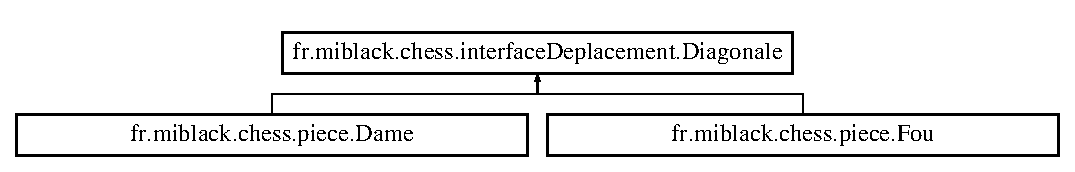
\includegraphics[height=1.866667cm]{interfacefr_1_1miblack_1_1chess_1_1interfaceDeplacement_1_1Diagonale}
\end{center}
\end{figure}
\subsection*{Public Member Functions}
\begin{DoxyCompactItemize}
\item 
Linked\-List$<$ {\bf Position} $>$ {\bf position\-Diagonale} ()
\end{DoxyCompactItemize}


\subsection{Detailed Description}
\begin{DoxyAuthor}{Author}
mi-\/black 
\end{DoxyAuthor}


\subsection{Member Function Documentation}
\index{fr\-::miblack\-::chess\-::interface\-Deplacement\-::\-Diagonale@{fr\-::miblack\-::chess\-::interface\-Deplacement\-::\-Diagonale}!position\-Diagonale@{position\-Diagonale}}
\index{position\-Diagonale@{position\-Diagonale}!fr::miblack::chess::interfaceDeplacement::Diagonale@{fr\-::miblack\-::chess\-::interface\-Deplacement\-::\-Diagonale}}
\subsubsection[{position\-Diagonale}]{\setlength{\rightskip}{0pt plus 5cm}Linked\-List$<${\bf Position}$>$ fr.\-miblack.\-chess.\-interface\-Deplacement.\-Diagonale.\-position\-Diagonale (
\begin{DoxyParamCaption}
{}
\end{DoxyParamCaption}
)}\label{interfacefr_1_1miblack_1_1chess_1_1interfaceDeplacement_1_1Diagonale_a4d6e3ca777cea05ea561875497ac1161}
\begin{DoxyReturn}{Returns}
liste des pos diagonales 
\end{DoxyReturn}


Implemented in {\bf fr.\-miblack.\-chess.\-piece.\-Dame} \doxyref{}{p.}{classfr_1_1miblack_1_1chess_1_1piece_1_1Dame_a6e03b316c8e420a3fab05f2afae4c677}, and {\bf fr.\-miblack.\-chess.\-piece.\-Fou} \doxyref{}{p.}{classfr_1_1miblack_1_1chess_1_1piece_1_1Fou_a60217f99d2d3569644351f9778761c54}.



The documentation for this interface was generated from the following file\-:\begin{DoxyCompactItemize}
\item 
fr/miblack/chess/interface\-Deplacement/Diagonale.\-java\end{DoxyCompactItemize}

\section{fr.\-miblack.\-chess.\-Echiquier Class Reference}
\label{classfr_1_1miblack_1_1chess_1_1Echiquier}\index{fr.\-miblack.\-chess.\-Echiquier@{fr.\-miblack.\-chess.\-Echiquier}}


Collaboration diagram for fr.\-miblack.\-chess.\-Echiquier\-:
\nopagebreak
\begin{figure}[H]
\begin{center}
\leavevmode
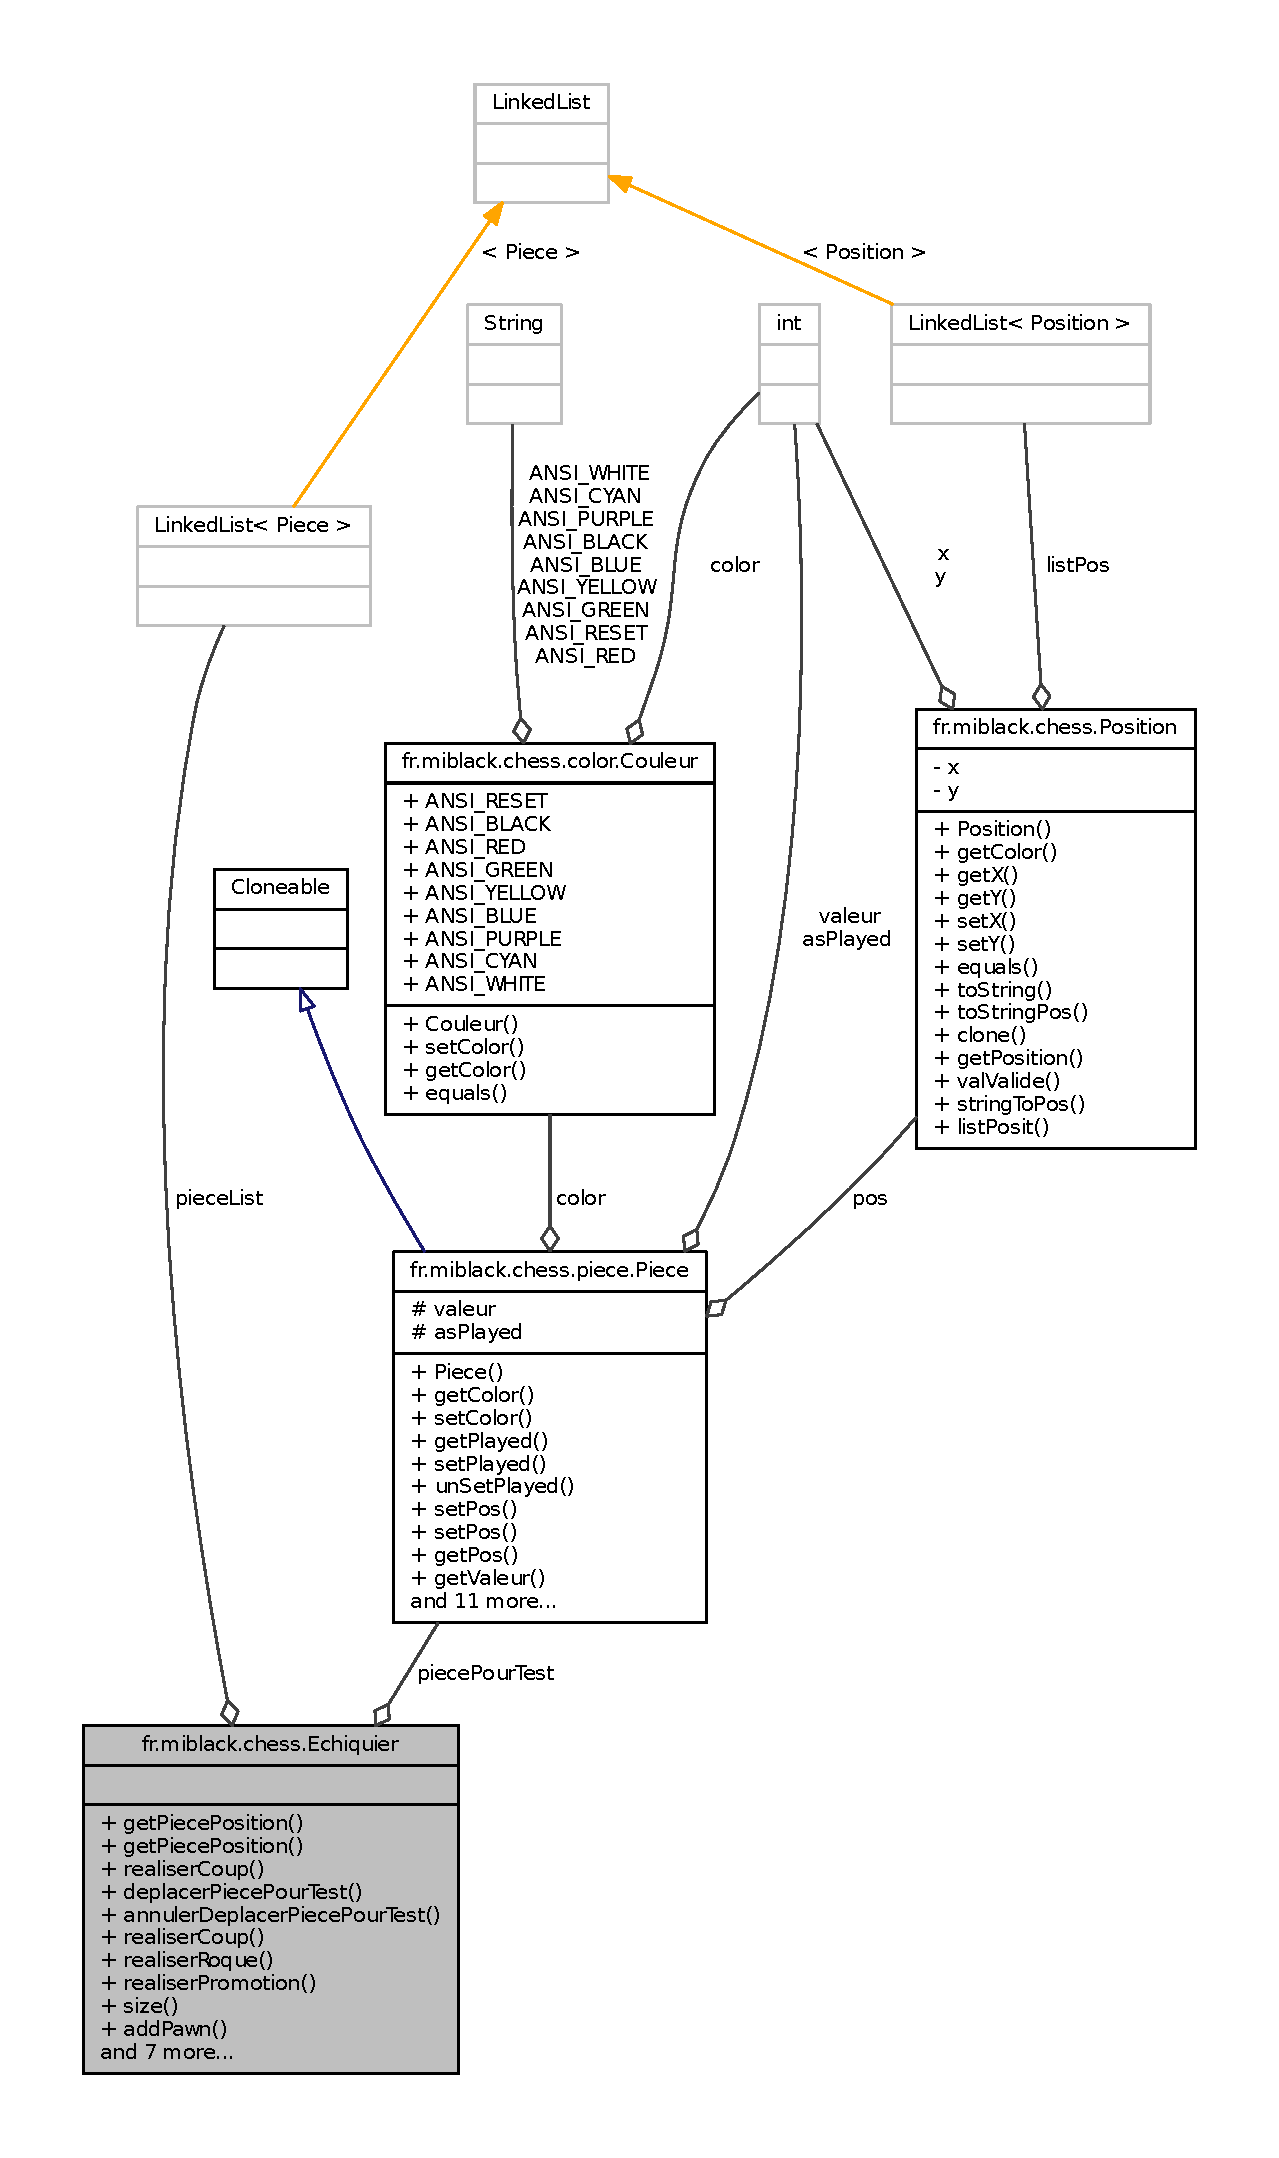
\includegraphics[height=550pt]{classfr_1_1miblack_1_1chess_1_1Echiquier__coll__graph}
\end{center}
\end{figure}
\subsection*{Public Member Functions}
\begin{DoxyCompactItemize}
\item 
{\bf Piece} {\bf get\-Piece\-Position} ({\bf Position} pos)
\item 
{\bf Piece} {\bf get\-Piece\-Position} (int x, int y)
\item 
boolean {\bf realiser\-Coup} ({\bf Piece} piece\-Depart, {\bf Position} pos\-Arrivee)
\item 
boolean {\bf deplacer\-Piece\-Pour\-Test} ({\bf Position} pos\-Depart, {\bf Position} pos\-Arrivee)
\item 
void {\bf annuler\-Deplacer\-Piece\-Pour\-Test} ({\bf Position} pos\-Depart, {\bf Position} pos\-Arrivee, boolean is\-Prise)
\item 
boolean {\bf realiser\-Coup} ({\bf Coup} my\-Coup)
\item 
void {\bf realiser\-Roque} ({\bf Coup} my\-Coup)
\item 
void {\bf realiser\-Promotion} ({\bf Coup} my\-Coup)
\item 
int {\bf size} ()
\item 
boolean {\bf add\-Pawn} ({\bf Pion} pawn)
\item 
boolean {\bf add\-Rook} (Tour rook)
\item 
boolean {\bf add\-Bishop} (Fou bishop)
\item 
boolean {\bf add\-King} (Roi king)
\item 
boolean {\bf add\-Knight} (Cavalier knight)
\item 
boolean {\bf add\-Queen} (Dame queen)
\item 
{\bf Position} {\bf get\-Position} (int x, int y)
\item 
Linked\-List$<$ {\bf Piece} $>$ {\bf get\-Piece\-List} ()
\end{DoxyCompactItemize}
\subsection*{Private Attributes}
\begin{DoxyCompactItemize}
\item 
Linked\-List$<$ {\bf Piece} $>$ {\bf piece\-List} = new Linked\-List$<${\bf Piece}$>$()
\item 
{\bf Piece} {\bf piece\-Pour\-Test}
\end{DoxyCompactItemize}


\subsection{Detailed Description}
Un echiquier est composé d'une liste de piece et d'une piece bidon (pour les test de déplacement

\begin{DoxyAuthor}{Author}
mi-\/black 
\end{DoxyAuthor}


\subsection{Member Function Documentation}
\index{fr\-::miblack\-::chess\-::\-Echiquier@{fr\-::miblack\-::chess\-::\-Echiquier}!add\-Bishop@{add\-Bishop}}
\index{add\-Bishop@{add\-Bishop}!fr::miblack::chess::Echiquier@{fr\-::miblack\-::chess\-::\-Echiquier}}
\subsubsection[{add\-Bishop}]{\setlength{\rightskip}{0pt plus 5cm}boolean fr.\-miblack.\-chess.\-Echiquier.\-add\-Bishop (
\begin{DoxyParamCaption}
\item[{Fou}]{bishop}
\end{DoxyParamCaption}
)}\label{classfr_1_1miblack_1_1chess_1_1Echiquier_a4da0881ba43b423f06c4508de8be6eab}

\begin{DoxyParams}{Parameters}
{\em bishop} & \\
\hline
\end{DoxyParams}
\begin{DoxyReturn}{Returns}
add un fou a la Linked\-List de piece 
\end{DoxyReturn}
\index{fr\-::miblack\-::chess\-::\-Echiquier@{fr\-::miblack\-::chess\-::\-Echiquier}!add\-King@{add\-King}}
\index{add\-King@{add\-King}!fr::miblack::chess::Echiquier@{fr\-::miblack\-::chess\-::\-Echiquier}}
\subsubsection[{add\-King}]{\setlength{\rightskip}{0pt plus 5cm}boolean fr.\-miblack.\-chess.\-Echiquier.\-add\-King (
\begin{DoxyParamCaption}
\item[{Roi}]{king}
\end{DoxyParamCaption}
)}\label{classfr_1_1miblack_1_1chess_1_1Echiquier_a8b5289564f41260ee69e5ab07ec3a40a}

\begin{DoxyParams}{Parameters}
{\em king} & \\
\hline
\end{DoxyParams}
\begin{DoxyReturn}{Returns}
add un roi a la Linked\-List de piece 
\end{DoxyReturn}
\index{fr\-::miblack\-::chess\-::\-Echiquier@{fr\-::miblack\-::chess\-::\-Echiquier}!add\-Knight@{add\-Knight}}
\index{add\-Knight@{add\-Knight}!fr::miblack::chess::Echiquier@{fr\-::miblack\-::chess\-::\-Echiquier}}
\subsubsection[{add\-Knight}]{\setlength{\rightskip}{0pt plus 5cm}boolean fr.\-miblack.\-chess.\-Echiquier.\-add\-Knight (
\begin{DoxyParamCaption}
\item[{Cavalier}]{knight}
\end{DoxyParamCaption}
)}\label{classfr_1_1miblack_1_1chess_1_1Echiquier_a06f442c6f0091c26747f27d39396c998}

\begin{DoxyParams}{Parameters}
{\em knight} & \\
\hline
\end{DoxyParams}
\begin{DoxyReturn}{Returns}
add un cavalier a la Linked\-List de piece 
\end{DoxyReturn}
\index{fr\-::miblack\-::chess\-::\-Echiquier@{fr\-::miblack\-::chess\-::\-Echiquier}!add\-Pawn@{add\-Pawn}}
\index{add\-Pawn@{add\-Pawn}!fr::miblack::chess::Echiquier@{fr\-::miblack\-::chess\-::\-Echiquier}}
\subsubsection[{add\-Pawn}]{\setlength{\rightskip}{0pt plus 5cm}boolean fr.\-miblack.\-chess.\-Echiquier.\-add\-Pawn (
\begin{DoxyParamCaption}
\item[{{\bf Pion}}]{pawn}
\end{DoxyParamCaption}
)}\label{classfr_1_1miblack_1_1chess_1_1Echiquier_a41400178a45844e34127af4763a201b9}

\begin{DoxyParams}{Parameters}
{\em pawn} & \\
\hline
\end{DoxyParams}
\begin{DoxyReturn}{Returns}
add un pion a la Linked\-List de piece 
\end{DoxyReturn}
\index{fr\-::miblack\-::chess\-::\-Echiquier@{fr\-::miblack\-::chess\-::\-Echiquier}!add\-Queen@{add\-Queen}}
\index{add\-Queen@{add\-Queen}!fr::miblack::chess::Echiquier@{fr\-::miblack\-::chess\-::\-Echiquier}}
\subsubsection[{add\-Queen}]{\setlength{\rightskip}{0pt plus 5cm}boolean fr.\-miblack.\-chess.\-Echiquier.\-add\-Queen (
\begin{DoxyParamCaption}
\item[{Dame}]{queen}
\end{DoxyParamCaption}
)}\label{classfr_1_1miblack_1_1chess_1_1Echiquier_a418ecee6543da45a8b7090be0bce0452}

\begin{DoxyParams}{Parameters}
{\em queen} & \\
\hline
\end{DoxyParams}
\begin{DoxyReturn}{Returns}
add une dame a la Linked\-List de piece 
\end{DoxyReturn}
\index{fr\-::miblack\-::chess\-::\-Echiquier@{fr\-::miblack\-::chess\-::\-Echiquier}!add\-Rook@{add\-Rook}}
\index{add\-Rook@{add\-Rook}!fr::miblack::chess::Echiquier@{fr\-::miblack\-::chess\-::\-Echiquier}}
\subsubsection[{add\-Rook}]{\setlength{\rightskip}{0pt plus 5cm}boolean fr.\-miblack.\-chess.\-Echiquier.\-add\-Rook (
\begin{DoxyParamCaption}
\item[{Tour}]{rook}
\end{DoxyParamCaption}
)}\label{classfr_1_1miblack_1_1chess_1_1Echiquier_a0732e2375a473b31c5a5d9bd6aa1d344}

\begin{DoxyParams}{Parameters}
{\em rook} & \\
\hline
\end{DoxyParams}
\begin{DoxyReturn}{Returns}
add une tour a la Linked\-List de piece 
\end{DoxyReturn}
\index{fr\-::miblack\-::chess\-::\-Echiquier@{fr\-::miblack\-::chess\-::\-Echiquier}!annuler\-Deplacer\-Piece\-Pour\-Test@{annuler\-Deplacer\-Piece\-Pour\-Test}}
\index{annuler\-Deplacer\-Piece\-Pour\-Test@{annuler\-Deplacer\-Piece\-Pour\-Test}!fr::miblack::chess::Echiquier@{fr\-::miblack\-::chess\-::\-Echiquier}}
\subsubsection[{annuler\-Deplacer\-Piece\-Pour\-Test}]{\setlength{\rightskip}{0pt plus 5cm}void fr.\-miblack.\-chess.\-Echiquier.\-annuler\-Deplacer\-Piece\-Pour\-Test (
\begin{DoxyParamCaption}
\item[{{\bf Position}}]{pos\-Depart, }
\item[{{\bf Position}}]{pos\-Arrivee, }
\item[{boolean}]{is\-Prise}
\end{DoxyParamCaption}
)}\label{classfr_1_1miblack_1_1chess_1_1Echiquier_a12f3a1f72412b772eb8beb6f50431c56}

\begin{DoxyParams}{Parameters}
{\em pos\-Depart} & \\
\hline
{\em pos\-Arrivee} & \\
\hline
{\em is\-Prise} & \\
\hline
\end{DoxyParams}
\index{fr\-::miblack\-::chess\-::\-Echiquier@{fr\-::miblack\-::chess\-::\-Echiquier}!deplacer\-Piece\-Pour\-Test@{deplacer\-Piece\-Pour\-Test}}
\index{deplacer\-Piece\-Pour\-Test@{deplacer\-Piece\-Pour\-Test}!fr::miblack::chess::Echiquier@{fr\-::miblack\-::chess\-::\-Echiquier}}
\subsubsection[{deplacer\-Piece\-Pour\-Test}]{\setlength{\rightskip}{0pt plus 5cm}boolean fr.\-miblack.\-chess.\-Echiquier.\-deplacer\-Piece\-Pour\-Test (
\begin{DoxyParamCaption}
\item[{{\bf Position}}]{pos\-Depart, }
\item[{{\bf Position}}]{pos\-Arrivee}
\end{DoxyParamCaption}
)}\label{classfr_1_1miblack_1_1chess_1_1Echiquier_a309c20c7c38cedb96d3b2c386d11ab4e}
Deplace une piece sans faire de test


\begin{DoxyParams}{Parameters}
{\em pos\-Depart} & \\
\hline
{\em pos\-Arrivee} & \\
\hline
\end{DoxyParams}
\begin{DoxyReturn}{Returns}
s'il y a une prise de piece 
\end{DoxyReturn}
\index{fr\-::miblack\-::chess\-::\-Echiquier@{fr\-::miblack\-::chess\-::\-Echiquier}!get\-Piece\-List@{get\-Piece\-List}}
\index{get\-Piece\-List@{get\-Piece\-List}!fr::miblack::chess::Echiquier@{fr\-::miblack\-::chess\-::\-Echiquier}}
\subsubsection[{get\-Piece\-List}]{\setlength{\rightskip}{0pt plus 5cm}Linked\-List$<${\bf Piece}$>$ fr.\-miblack.\-chess.\-Echiquier.\-get\-Piece\-List (
\begin{DoxyParamCaption}
{}
\end{DoxyParamCaption}
)}\label{classfr_1_1miblack_1_1chess_1_1Echiquier_a06b5c21ea48b6a8655c093e9d502d308}
\begin{DoxyReturn}{Returns}
get la liste de piece 
\end{DoxyReturn}
\index{fr\-::miblack\-::chess\-::\-Echiquier@{fr\-::miblack\-::chess\-::\-Echiquier}!get\-Piece\-Position@{get\-Piece\-Position}}
\index{get\-Piece\-Position@{get\-Piece\-Position}!fr::miblack::chess::Echiquier@{fr\-::miblack\-::chess\-::\-Echiquier}}
\subsubsection[{get\-Piece\-Position}]{\setlength{\rightskip}{0pt plus 5cm}{\bf Piece} fr.\-miblack.\-chess.\-Echiquier.\-get\-Piece\-Position (
\begin{DoxyParamCaption}
\item[{{\bf Position}}]{pos}
\end{DoxyParamCaption}
)}\label{classfr_1_1miblack_1_1chess_1_1Echiquier_aa01d1868aefe9f4fe33a7b8955844867}

\begin{DoxyParams}{Parameters}
{\em pos} & \\
\hline
\end{DoxyParams}
\begin{DoxyReturn}{Returns}
la piece a la position donnee , null si la position est vide 
\end{DoxyReturn}
\index{fr\-::miblack\-::chess\-::\-Echiquier@{fr\-::miblack\-::chess\-::\-Echiquier}!get\-Piece\-Position@{get\-Piece\-Position}}
\index{get\-Piece\-Position@{get\-Piece\-Position}!fr::miblack::chess::Echiquier@{fr\-::miblack\-::chess\-::\-Echiquier}}
\subsubsection[{get\-Piece\-Position}]{\setlength{\rightskip}{0pt plus 5cm}{\bf Piece} fr.\-miblack.\-chess.\-Echiquier.\-get\-Piece\-Position (
\begin{DoxyParamCaption}
\item[{int}]{x, }
\item[{int}]{y}
\end{DoxyParamCaption}
)}\label{classfr_1_1miblack_1_1chess_1_1Echiquier_aa0fa7c0675f642cae8fbf881416ee854}
Retourne la piece positionné a telle coordonnée x \& y 
\begin{DoxyParams}{Parameters}
{\em x} & \\
\hline
{\em y} & \\
\hline
\end{DoxyParams}
\begin{DoxyReturn}{Returns}
la piece a la position donnee , null si la position est vide 
\end{DoxyReturn}
\index{fr\-::miblack\-::chess\-::\-Echiquier@{fr\-::miblack\-::chess\-::\-Echiquier}!get\-Position@{get\-Position}}
\index{get\-Position@{get\-Position}!fr::miblack::chess::Echiquier@{fr\-::miblack\-::chess\-::\-Echiquier}}
\subsubsection[{get\-Position}]{\setlength{\rightskip}{0pt plus 5cm}{\bf Position} fr.\-miblack.\-chess.\-Echiquier.\-get\-Position (
\begin{DoxyParamCaption}
\item[{int}]{x, }
\item[{int}]{y}
\end{DoxyParamCaption}
)}\label{classfr_1_1miblack_1_1chess_1_1Echiquier_a22c73b19bc9e4333e79221799acb060e}
Le fly-\/weight de position 
\begin{DoxyParams}{Parameters}
{\em x} & \\
\hline
{\em y} & \\
\hline
\end{DoxyParams}
\begin{DoxyReturn}{Returns}
Position.\-get\-Position( x, y ) 
\end{DoxyReturn}
\index{fr\-::miblack\-::chess\-::\-Echiquier@{fr\-::miblack\-::chess\-::\-Echiquier}!realiser\-Coup@{realiser\-Coup}}
\index{realiser\-Coup@{realiser\-Coup}!fr::miblack::chess::Echiquier@{fr\-::miblack\-::chess\-::\-Echiquier}}
\subsubsection[{realiser\-Coup}]{\setlength{\rightskip}{0pt plus 5cm}boolean fr.\-miblack.\-chess.\-Echiquier.\-realiser\-Coup (
\begin{DoxyParamCaption}
\item[{{\bf Piece}}]{piece\-Depart, }
\item[{{\bf Position}}]{pos\-Arrivee}
\end{DoxyParamCaption}
)}\label{classfr_1_1miblack_1_1chess_1_1Echiquier_acc1dce24fe3efb55bdd3c458385fdf43}
Deplacer la piece un coup,


\begin{DoxyParams}{Parameters}
{\em piece\-Depart} & \\
\hline
{\em pos\-Arrivee} & \\
\hline
\end{DoxyParams}
\begin{DoxyReturn}{Returns}

\end{DoxyReturn}
\index{fr\-::miblack\-::chess\-::\-Echiquier@{fr\-::miblack\-::chess\-::\-Echiquier}!realiser\-Coup@{realiser\-Coup}}
\index{realiser\-Coup@{realiser\-Coup}!fr::miblack::chess::Echiquier@{fr\-::miblack\-::chess\-::\-Echiquier}}
\subsubsection[{realiser\-Coup}]{\setlength{\rightskip}{0pt plus 5cm}boolean fr.\-miblack.\-chess.\-Echiquier.\-realiser\-Coup (
\begin{DoxyParamCaption}
\item[{{\bf Coup}}]{my\-Coup}
\end{DoxyParamCaption}
)}\label{classfr_1_1miblack_1_1chess_1_1Echiquier_a7766d5a2d057c48cfffd6c3eab41dd83}
Realise un déplacement 
\begin{DoxyParams}{Parameters}
{\em my\-Coup} & \\
\hline
\end{DoxyParams}
\begin{DoxyReturn}{Returns}

\end{DoxyReturn}
\index{fr\-::miblack\-::chess\-::\-Echiquier@{fr\-::miblack\-::chess\-::\-Echiquier}!realiser\-Promotion@{realiser\-Promotion}}
\index{realiser\-Promotion@{realiser\-Promotion}!fr::miblack::chess::Echiquier@{fr\-::miblack\-::chess\-::\-Echiquier}}
\subsubsection[{realiser\-Promotion}]{\setlength{\rightskip}{0pt plus 5cm}void fr.\-miblack.\-chess.\-Echiquier.\-realiser\-Promotion (
\begin{DoxyParamCaption}
\item[{{\bf Coup}}]{my\-Coup}
\end{DoxyParamCaption}
)}\label{classfr_1_1miblack_1_1chess_1_1Echiquier_a8284522759957e949ff34b8730a41a76}
Realise la promotion (change la piece) 
\begin{DoxyParams}{Parameters}
{\em my\-Coup} & \\
\hline
\end{DoxyParams}
\index{fr\-::miblack\-::chess\-::\-Echiquier@{fr\-::miblack\-::chess\-::\-Echiquier}!realiser\-Roque@{realiser\-Roque}}
\index{realiser\-Roque@{realiser\-Roque}!fr::miblack::chess::Echiquier@{fr\-::miblack\-::chess\-::\-Echiquier}}
\subsubsection[{realiser\-Roque}]{\setlength{\rightskip}{0pt plus 5cm}void fr.\-miblack.\-chess.\-Echiquier.\-realiser\-Roque (
\begin{DoxyParamCaption}
\item[{{\bf Coup}}]{my\-Coup}
\end{DoxyParamCaption}
)}\label{classfr_1_1miblack_1_1chess_1_1Echiquier_a2437836a49536775ad6e344ab176cfa3}
Realise le roque (deplace les pieces) 
\begin{DoxyParams}{Parameters}
{\em my\-Coup} & (le coup joue) \\
\hline
\end{DoxyParams}
\index{fr\-::miblack\-::chess\-::\-Echiquier@{fr\-::miblack\-::chess\-::\-Echiquier}!size@{size}}
\index{size@{size}!fr::miblack::chess::Echiquier@{fr\-::miblack\-::chess\-::\-Echiquier}}
\subsubsection[{size}]{\setlength{\rightskip}{0pt plus 5cm}int fr.\-miblack.\-chess.\-Echiquier.\-size (
\begin{DoxyParamCaption}
{}
\end{DoxyParamCaption}
)}\label{classfr_1_1miblack_1_1chess_1_1Echiquier_a5093766638d061cd0b65f3a2f9e3bf0b}
\begin{DoxyReturn}{Returns}
piece\-List.\-size() 
\end{DoxyReturn}


\subsection{Member Data Documentation}
\index{fr\-::miblack\-::chess\-::\-Echiquier@{fr\-::miblack\-::chess\-::\-Echiquier}!piece\-List@{piece\-List}}
\index{piece\-List@{piece\-List}!fr::miblack::chess::Echiquier@{fr\-::miblack\-::chess\-::\-Echiquier}}
\subsubsection[{piece\-List}]{\setlength{\rightskip}{0pt plus 5cm}Linked\-List$<${\bf Piece}$>$ fr.\-miblack.\-chess.\-Echiquier.\-piece\-List = new Linked\-List$<${\bf Piece}$>$()\hspace{0.3cm}{\ttfamily [private]}}\label{classfr_1_1miblack_1_1chess_1_1Echiquier_a843137b4575f2ffd5bb6e91b6b0f6087}
\index{fr\-::miblack\-::chess\-::\-Echiquier@{fr\-::miblack\-::chess\-::\-Echiquier}!piece\-Pour\-Test@{piece\-Pour\-Test}}
\index{piece\-Pour\-Test@{piece\-Pour\-Test}!fr::miblack::chess::Echiquier@{fr\-::miblack\-::chess\-::\-Echiquier}}
\subsubsection[{piece\-Pour\-Test}]{\setlength{\rightskip}{0pt plus 5cm}{\bf Piece} fr.\-miblack.\-chess.\-Echiquier.\-piece\-Pour\-Test\hspace{0.3cm}{\ttfamily [private]}}\label{classfr_1_1miblack_1_1chess_1_1Echiquier_a2cd0b5d5c607b02b7de74607809e4d87}


The documentation for this class was generated from the following file\-:\begin{DoxyCompactItemize}
\item 
fr/miblack/chess/{\bf Echiquier.\-java}\end{DoxyCompactItemize}

\section{fr.\-miblack.\-chess.\-affichage.\-G\-U\-I.\-Echiquier\-Graphique Class Reference}
\label{classfr_1_1miblack_1_1chess_1_1affichage_1_1GUI_1_1EchiquierGraphique}\index{fr.\-miblack.\-chess.\-affichage.\-G\-U\-I.\-Echiquier\-Graphique@{fr.\-miblack.\-chess.\-affichage.\-G\-U\-I.\-Echiquier\-Graphique}}


Inheritance diagram for fr.\-miblack.\-chess.\-affichage.\-G\-U\-I.\-Echiquier\-Graphique\-:
\nopagebreak
\begin{figure}[H]
\begin{center}
\leavevmode
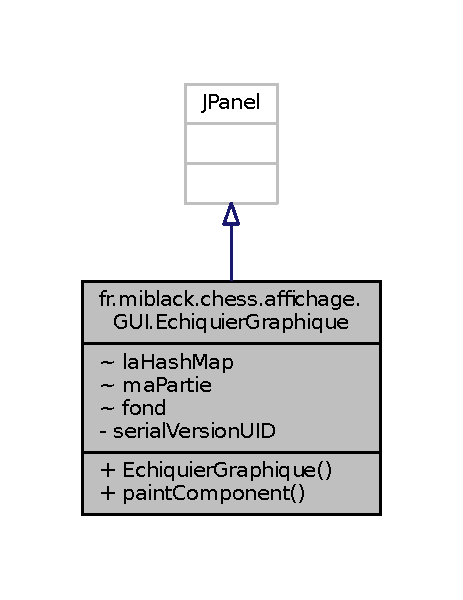
\includegraphics[width=222pt]{classfr_1_1miblack_1_1chess_1_1affichage_1_1GUI_1_1EchiquierGraphique__inherit__graph}
\end{center}
\end{figure}


Collaboration diagram for fr.\-miblack.\-chess.\-affichage.\-G\-U\-I.\-Echiquier\-Graphique\-:
\nopagebreak
\begin{figure}[H]
\begin{center}
\leavevmode
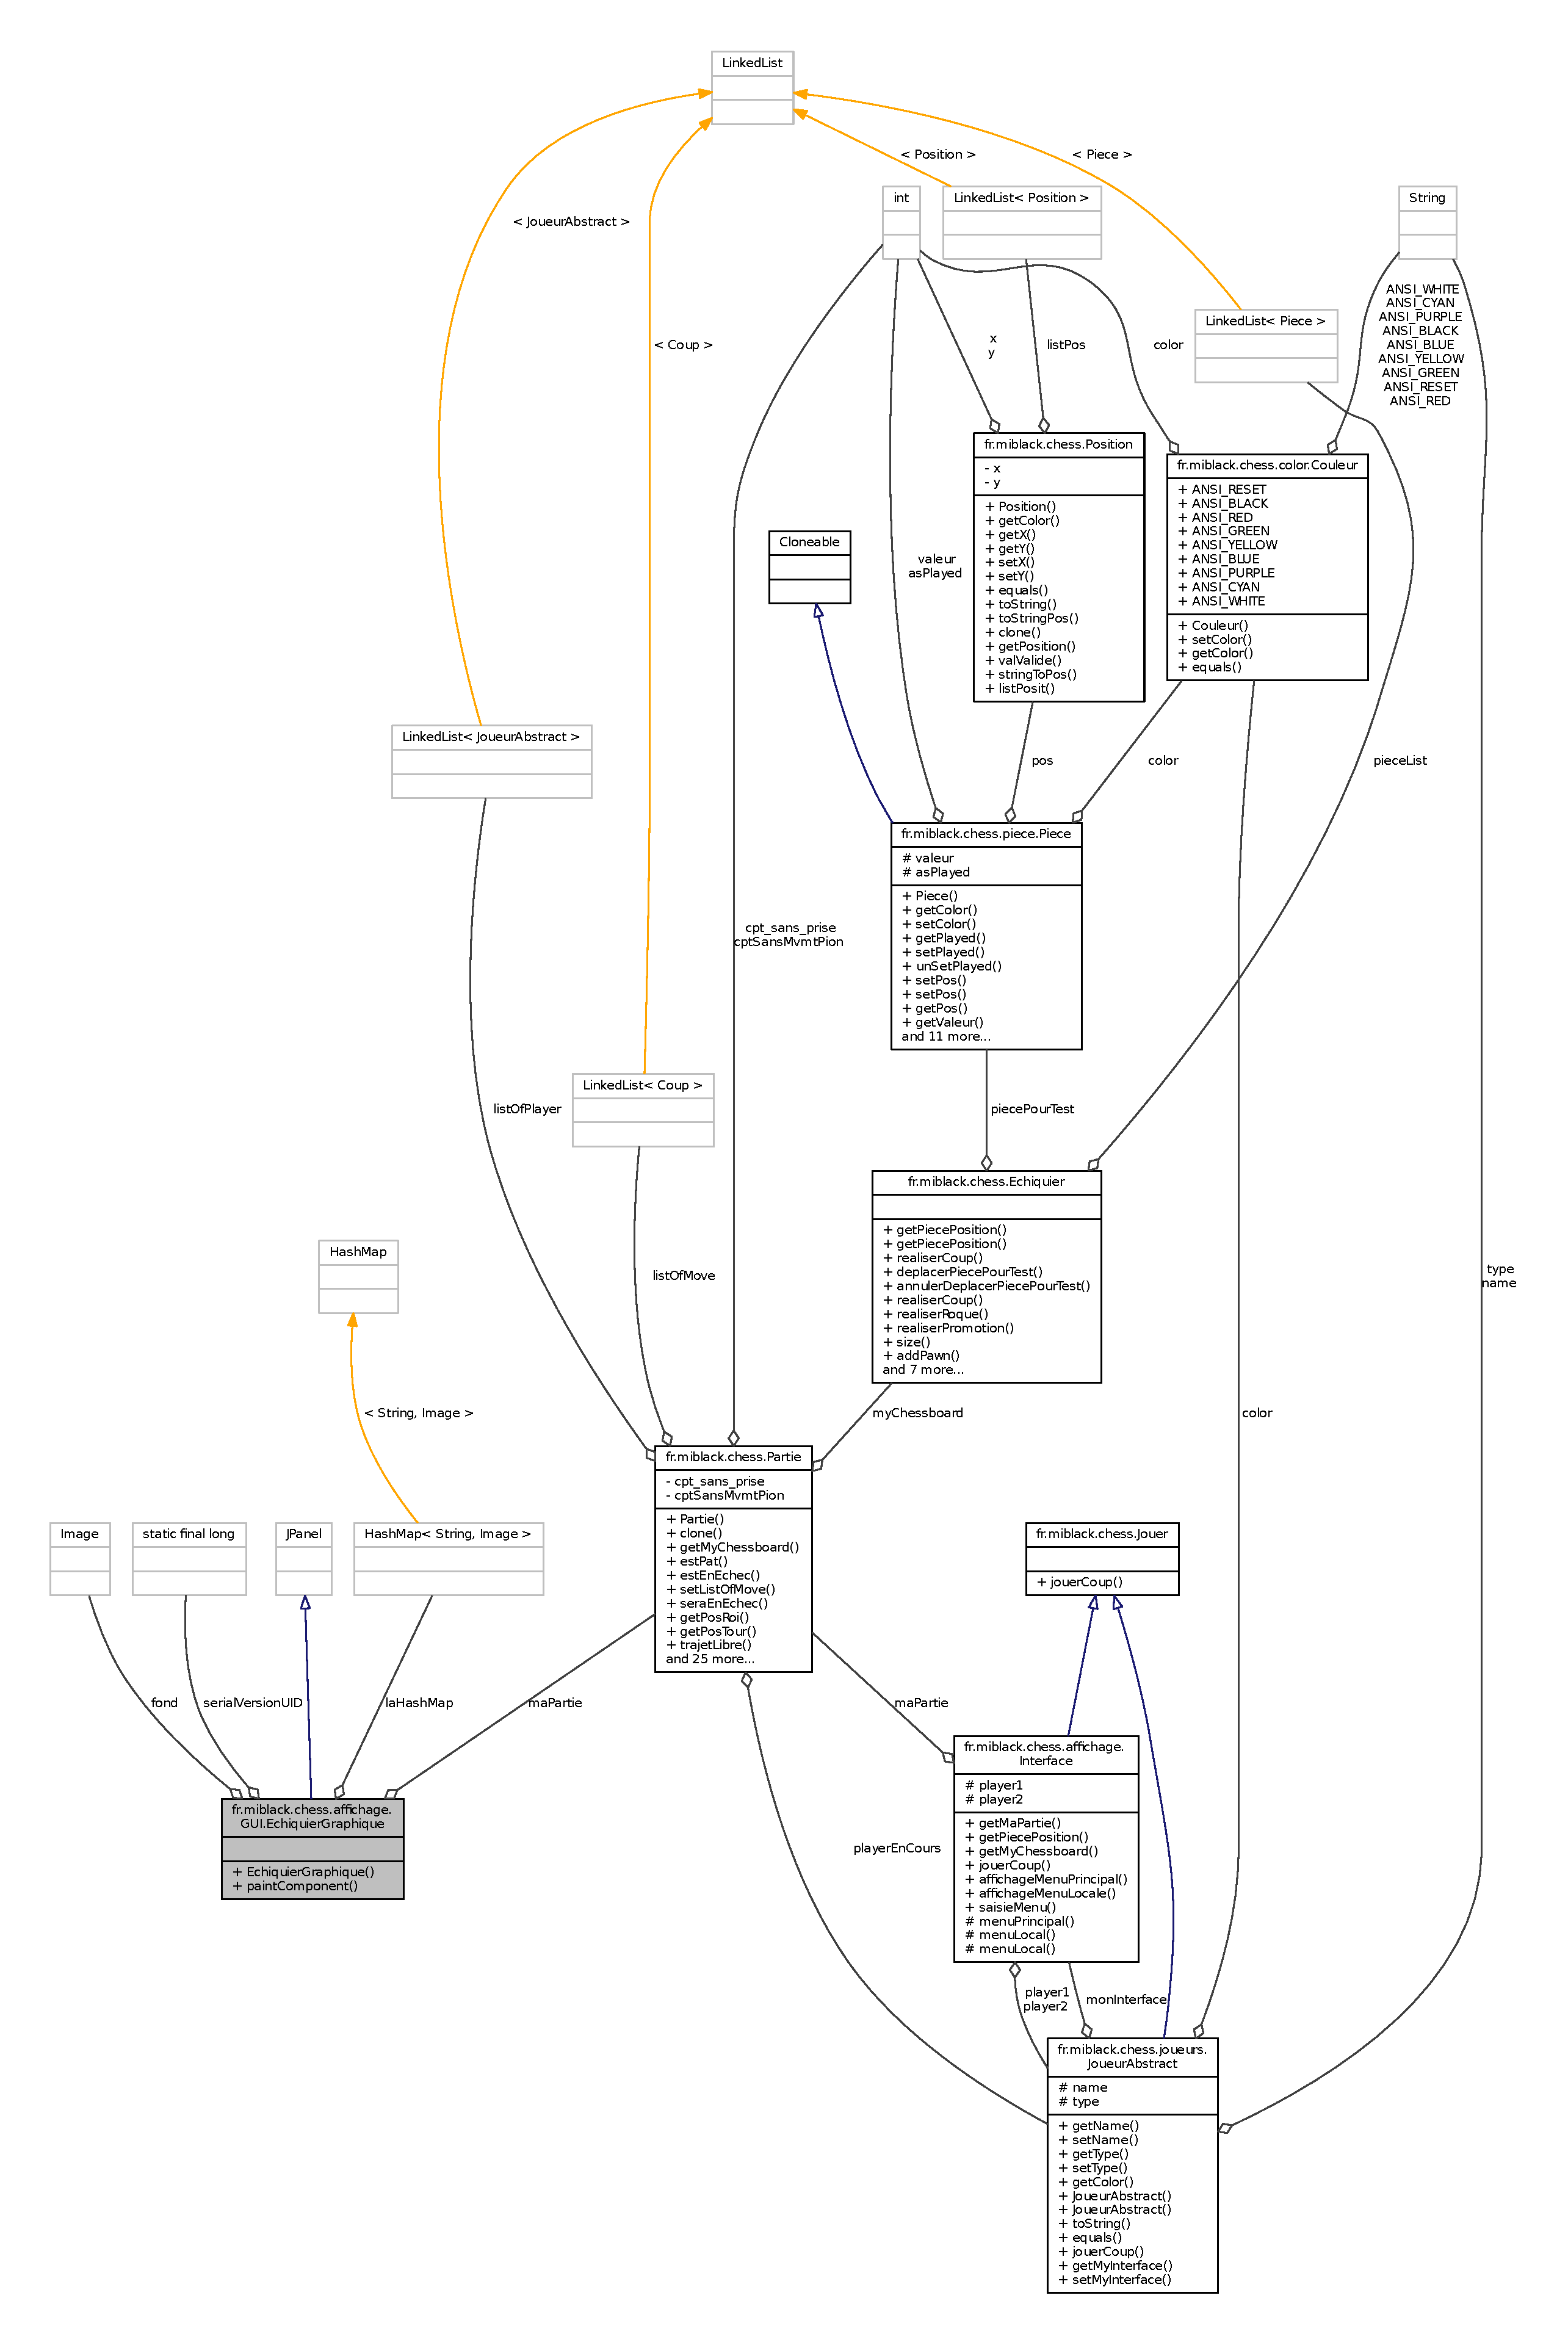
\includegraphics[width=350pt]{classfr_1_1miblack_1_1chess_1_1affichage_1_1GUI_1_1EchiquierGraphique__coll__graph}
\end{center}
\end{figure}
\subsection*{Public Member Functions}
\begin{DoxyCompactItemize}
\item 
{\bf Echiquier\-Graphique} ({\bf Partie} ma\-Partie)
\item 
void {\bf paint\-Component} (Graphics g)
\end{DoxyCompactItemize}
\subsection*{Static Private Attributes}
\begin{DoxyCompactItemize}
\item 
static final long {\bf serial\-Version\-U\-I\-D} = 1\-L
\end{DoxyCompactItemize}


\subsection{Detailed Description}
\begin{DoxyAuthor}{Author}
mi-\/black 
\end{DoxyAuthor}


\subsection{Constructor \& Destructor Documentation}
\index{fr\-::miblack\-::chess\-::affichage\-::\-G\-U\-I\-::\-Echiquier\-Graphique@{fr\-::miblack\-::chess\-::affichage\-::\-G\-U\-I\-::\-Echiquier\-Graphique}!Echiquier\-Graphique@{Echiquier\-Graphique}}
\index{Echiquier\-Graphique@{Echiquier\-Graphique}!fr::miblack::chess::affichage::GUI::EchiquierGraphique@{fr\-::miblack\-::chess\-::affichage\-::\-G\-U\-I\-::\-Echiquier\-Graphique}}
\subsubsection[{Echiquier\-Graphique}]{\setlength{\rightskip}{0pt plus 5cm}fr.\-miblack.\-chess.\-affichage.\-G\-U\-I.\-Echiquier\-Graphique.\-Echiquier\-Graphique (
\begin{DoxyParamCaption}
\item[{{\bf Partie}}]{ma\-Partie}
\end{DoxyParamCaption}
)}\label{classfr_1_1miblack_1_1chess_1_1affichage_1_1GUI_1_1EchiquierGraphique_a10214d304fe48126760cd55694982e52}

\begin{DoxyParams}{Parameters}
{\em ma\-Partie} & \\
\hline
\end{DoxyParams}


\subsection{Member Function Documentation}
\index{fr\-::miblack\-::chess\-::affichage\-::\-G\-U\-I\-::\-Echiquier\-Graphique@{fr\-::miblack\-::chess\-::affichage\-::\-G\-U\-I\-::\-Echiquier\-Graphique}!paint\-Component@{paint\-Component}}
\index{paint\-Component@{paint\-Component}!fr::miblack::chess::affichage::GUI::EchiquierGraphique@{fr\-::miblack\-::chess\-::affichage\-::\-G\-U\-I\-::\-Echiquier\-Graphique}}
\subsubsection[{paint\-Component}]{\setlength{\rightskip}{0pt plus 5cm}void fr.\-miblack.\-chess.\-affichage.\-G\-U\-I.\-Echiquier\-Graphique.\-paint\-Component (
\begin{DoxyParamCaption}
\item[{Graphics}]{g}
\end{DoxyParamCaption}
)}\label{classfr_1_1miblack_1_1chess_1_1affichage_1_1GUI_1_1EchiquierGraphique_a4ea692d0591c89885f1793860a13abad}

\begin{DoxyParams}{Parameters}
{\em g} & \\
\hline
\end{DoxyParams}


\subsection{Member Data Documentation}
\index{fr\-::miblack\-::chess\-::affichage\-::\-G\-U\-I\-::\-Echiquier\-Graphique@{fr\-::miblack\-::chess\-::affichage\-::\-G\-U\-I\-::\-Echiquier\-Graphique}!serial\-Version\-U\-I\-D@{serial\-Version\-U\-I\-D}}
\index{serial\-Version\-U\-I\-D@{serial\-Version\-U\-I\-D}!fr::miblack::chess::affichage::GUI::EchiquierGraphique@{fr\-::miblack\-::chess\-::affichage\-::\-G\-U\-I\-::\-Echiquier\-Graphique}}
\subsubsection[{serial\-Version\-U\-I\-D}]{\setlength{\rightskip}{0pt plus 5cm}final long fr.\-miblack.\-chess.\-affichage.\-G\-U\-I.\-Echiquier\-Graphique.\-serial\-Version\-U\-I\-D = 1\-L\hspace{0.3cm}{\ttfamily [static]}, {\ttfamily [private]}}\label{classfr_1_1miblack_1_1chess_1_1affichage_1_1GUI_1_1EchiquierGraphique_abeccd3f8e010c0e90a47ed2084471f9c}


The documentation for this class was generated from the following file\-:\begin{DoxyCompactItemize}
\item 
fr/miblack/chess/affichage/\-G\-U\-I/{\bf Echiquier\-Graphique.\-java}\end{DoxyCompactItemize}

\section{fr.\-miblack.\-chess.\-affichage.\-G\-U\-I.\-Fenetre Class Reference}
\label{classfr_1_1miblack_1_1chess_1_1affichage_1_1GUI_1_1Fenetre}\index{fr.\-miblack.\-chess.\-affichage.\-G\-U\-I.\-Fenetre@{fr.\-miblack.\-chess.\-affichage.\-G\-U\-I.\-Fenetre}}


Inherits J\-Frame.

\subsection*{Classes}
\begin{DoxyCompactItemize}
\item 
class {\bfseries Afficher\-Astuce}
\item 
class {\bfseries Bouton\-Listener}
\item 
class {\bfseries Charger\-Partie}
\item 
class {\bfseries Clavier\-Listener}
\item 
class {\bfseries Sauvegarder\-Partie}
\item 
class {\bfseries Text\-Panel}
\item 
class {\bfseries Text\-Panel2}
\end{DoxyCompactItemize}
\subsection*{Public Member Functions}
\begin{DoxyCompactItemize}
\item 
{\bf Fenetre} ({\bf Partie} ma\-Partie)
\item 
void {\bf initialiser\-Fenetre} ()
\item 
{\bf Echiquier\-Graphique} {\bf get\-Mon\-Echiquier} ()
\item 
void {\bf set\-Mon\-Echiquier} ({\bf Echiquier\-Graphique} mon\-Echiquier)
\item 
J\-Text\-Area {\bf get\-Zone\-Saisie} ()
\item 
void {\bf set\-Zone\-Saisie} (J\-Text\-Area zone\-Saisie)
\item 
{\bf Partie} {\bf get\-Ma\-Partie} ()
\item 
void {\bf set\-Ma\-Partie} ({\bf Partie} ma\-Partie)
\item 
J\-Panel {\bf get\-Mon\-Panel} ()
\item 
void {\bf set\-Mon\-Panel} (J\-Panel mon\-Panel)
\item 
J\-Panel {\bf get\-Sud} ()
\item 
void {\bf set\-Sud} (J\-Panel sud)
\item 
J\-Button {\bf get\-Bouton\-Send} ()
\item 
void {\bf set\-Bouton\-Send} (J\-Button bouton\-Send)
\item 
String {\bf get\-Chaine} ()
\item 
void {\bf set\-Chaine} (String chaine)
\item 
J\-Panel {\bf get\-Nord} ()
\item 
{\bf Panneau\-Affichage\-Joueur} {\bf get\-Panneau\-Affichage} ()
\item 
void {\bf set\-Panneau\-Affichage} ({\bf Panneau\-Affichage\-Joueur} panneau\-Affichage)
\item 
void {\bf set\-Nord} (J\-Panel nord)
\item 
J\-Panel {\bf get\-Est} ()
\item 
void {\bf set\-Est} (J\-Panel est)
\item 
J\-Menu\-Item {\bf get\-Save} ()
\item 
void {\bf set\-Save} (J\-Menu\-Item save)
\item 
J\-Text\-Area {\bf get\-Msg} ()
\item 
void {\bf set\-Msg} (J\-Text\-Area {\bf msg})
\item 
J\-Text\-Area {\bf get\-Txt} ()
\item 
void {\bf set\-Txt} (J\-Text\-Area {\bf msg})
\item 
{\bf Fenetre} {\bf clone} ()
\item 
J\-Panel {\bf get\-Ouest} ()
\item 
void {\bf set\-Ouest} (J\-Panel ouest)
\item 
Text\-Panel2 {\bf get\-Liste\-Coup\-Jouable} ()
\item 
void {\bf set\-Liste\-Coup\-Jouable} (Text\-Panel2 liste\-Coup\-Jouable)
\end{DoxyCompactItemize}
\subsection*{Static Public Attributes}
\begin{DoxyCompactItemize}
\item 
static J\-Text\-Area {\bf msg}
\item 
static J\-Text\-Area {\bf txt}
\end{DoxyCompactItemize}


\subsection{Detailed Description}
\begin{DoxyAuthor}{Author}
mi-\/black 
\end{DoxyAuthor}


\subsection{Constructor \& Destructor Documentation}
\index{fr\-::miblack\-::chess\-::affichage\-::\-G\-U\-I\-::\-Fenetre@{fr\-::miblack\-::chess\-::affichage\-::\-G\-U\-I\-::\-Fenetre}!Fenetre@{Fenetre}}
\index{Fenetre@{Fenetre}!fr::miblack::chess::affichage::GUI::Fenetre@{fr\-::miblack\-::chess\-::affichage\-::\-G\-U\-I\-::\-Fenetre}}
\subsubsection[{Fenetre}]{\setlength{\rightskip}{0pt plus 5cm}fr.\-miblack.\-chess.\-affichage.\-G\-U\-I.\-Fenetre.\-Fenetre (
\begin{DoxyParamCaption}
\item[{{\bf Partie}}]{ma\-Partie}
\end{DoxyParamCaption}
)}\label{classfr_1_1miblack_1_1chess_1_1affichage_1_1GUI_1_1Fenetre_ac2cdb21e0c225a0765d4d2ae5869bb8c}

\begin{DoxyParams}{Parameters}
{\em ma\-Partie} & \\
\hline
\end{DoxyParams}


\subsection{Member Function Documentation}
\index{fr\-::miblack\-::chess\-::affichage\-::\-G\-U\-I\-::\-Fenetre@{fr\-::miblack\-::chess\-::affichage\-::\-G\-U\-I\-::\-Fenetre}!clone@{clone}}
\index{clone@{clone}!fr::miblack::chess::affichage::GUI::Fenetre@{fr\-::miblack\-::chess\-::affichage\-::\-G\-U\-I\-::\-Fenetre}}
\subsubsection[{clone}]{\setlength{\rightskip}{0pt plus 5cm}{\bf Fenetre} fr.\-miblack.\-chess.\-affichage.\-G\-U\-I.\-Fenetre.\-clone (
\begin{DoxyParamCaption}
{}
\end{DoxyParamCaption}
)}\label{classfr_1_1miblack_1_1chess_1_1affichage_1_1GUI_1_1Fenetre_ab6a7c3d38491135f6f3bdd19863a8508}
\begin{DoxyReturn}{Returns}

\end{DoxyReturn}
\index{fr\-::miblack\-::chess\-::affichage\-::\-G\-U\-I\-::\-Fenetre@{fr\-::miblack\-::chess\-::affichage\-::\-G\-U\-I\-::\-Fenetre}!get\-Bouton\-Send@{get\-Bouton\-Send}}
\index{get\-Bouton\-Send@{get\-Bouton\-Send}!fr::miblack::chess::affichage::GUI::Fenetre@{fr\-::miblack\-::chess\-::affichage\-::\-G\-U\-I\-::\-Fenetre}}
\subsubsection[{get\-Bouton\-Send}]{\setlength{\rightskip}{0pt plus 5cm}J\-Button fr.\-miblack.\-chess.\-affichage.\-G\-U\-I.\-Fenetre.\-get\-Bouton\-Send (
\begin{DoxyParamCaption}
{}
\end{DoxyParamCaption}
)}\label{classfr_1_1miblack_1_1chess_1_1affichage_1_1GUI_1_1Fenetre_a030194e558cf30046313402fbf542287}
\begin{DoxyReturn}{Returns}

\end{DoxyReturn}
\index{fr\-::miblack\-::chess\-::affichage\-::\-G\-U\-I\-::\-Fenetre@{fr\-::miblack\-::chess\-::affichage\-::\-G\-U\-I\-::\-Fenetre}!get\-Chaine@{get\-Chaine}}
\index{get\-Chaine@{get\-Chaine}!fr::miblack::chess::affichage::GUI::Fenetre@{fr\-::miblack\-::chess\-::affichage\-::\-G\-U\-I\-::\-Fenetre}}
\subsubsection[{get\-Chaine}]{\setlength{\rightskip}{0pt plus 5cm}String fr.\-miblack.\-chess.\-affichage.\-G\-U\-I.\-Fenetre.\-get\-Chaine (
\begin{DoxyParamCaption}
{}
\end{DoxyParamCaption}
)}\label{classfr_1_1miblack_1_1chess_1_1affichage_1_1GUI_1_1Fenetre_a436bf3df28e6f6b9a121e87d932d8791}
\begin{DoxyReturn}{Returns}

\end{DoxyReturn}
\index{fr\-::miblack\-::chess\-::affichage\-::\-G\-U\-I\-::\-Fenetre@{fr\-::miblack\-::chess\-::affichage\-::\-G\-U\-I\-::\-Fenetre}!get\-Est@{get\-Est}}
\index{get\-Est@{get\-Est}!fr::miblack::chess::affichage::GUI::Fenetre@{fr\-::miblack\-::chess\-::affichage\-::\-G\-U\-I\-::\-Fenetre}}
\subsubsection[{get\-Est}]{\setlength{\rightskip}{0pt plus 5cm}J\-Panel fr.\-miblack.\-chess.\-affichage.\-G\-U\-I.\-Fenetre.\-get\-Est (
\begin{DoxyParamCaption}
{}
\end{DoxyParamCaption}
)}\label{classfr_1_1miblack_1_1chess_1_1affichage_1_1GUI_1_1Fenetre_a2cbbd3d5b8e12ec960a63ab9173b0202}
\begin{DoxyReturn}{Returns}

\end{DoxyReturn}
\index{fr\-::miblack\-::chess\-::affichage\-::\-G\-U\-I\-::\-Fenetre@{fr\-::miblack\-::chess\-::affichage\-::\-G\-U\-I\-::\-Fenetre}!get\-Liste\-Coup\-Jouable@{get\-Liste\-Coup\-Jouable}}
\index{get\-Liste\-Coup\-Jouable@{get\-Liste\-Coup\-Jouable}!fr::miblack::chess::affichage::GUI::Fenetre@{fr\-::miblack\-::chess\-::affichage\-::\-G\-U\-I\-::\-Fenetre}}
\subsubsection[{get\-Liste\-Coup\-Jouable}]{\setlength{\rightskip}{0pt plus 5cm}Text\-Panel2 fr.\-miblack.\-chess.\-affichage.\-G\-U\-I.\-Fenetre.\-get\-Liste\-Coup\-Jouable (
\begin{DoxyParamCaption}
{}
\end{DoxyParamCaption}
)}\label{classfr_1_1miblack_1_1chess_1_1affichage_1_1GUI_1_1Fenetre_a745b9e97b06b22585ccda7d37250a9ff}
\begin{DoxyReturn}{Returns}

\end{DoxyReturn}
\index{fr\-::miblack\-::chess\-::affichage\-::\-G\-U\-I\-::\-Fenetre@{fr\-::miblack\-::chess\-::affichage\-::\-G\-U\-I\-::\-Fenetre}!get\-Ma\-Partie@{get\-Ma\-Partie}}
\index{get\-Ma\-Partie@{get\-Ma\-Partie}!fr::miblack::chess::affichage::GUI::Fenetre@{fr\-::miblack\-::chess\-::affichage\-::\-G\-U\-I\-::\-Fenetre}}
\subsubsection[{get\-Ma\-Partie}]{\setlength{\rightskip}{0pt plus 5cm}{\bf Partie} fr.\-miblack.\-chess.\-affichage.\-G\-U\-I.\-Fenetre.\-get\-Ma\-Partie (
\begin{DoxyParamCaption}
{}
\end{DoxyParamCaption}
)}\label{classfr_1_1miblack_1_1chess_1_1affichage_1_1GUI_1_1Fenetre_a307375f348e5961857099ba375274c21}
\begin{DoxyReturn}{Returns}

\end{DoxyReturn}
\index{fr\-::miblack\-::chess\-::affichage\-::\-G\-U\-I\-::\-Fenetre@{fr\-::miblack\-::chess\-::affichage\-::\-G\-U\-I\-::\-Fenetre}!get\-Mon\-Echiquier@{get\-Mon\-Echiquier}}
\index{get\-Mon\-Echiquier@{get\-Mon\-Echiquier}!fr::miblack::chess::affichage::GUI::Fenetre@{fr\-::miblack\-::chess\-::affichage\-::\-G\-U\-I\-::\-Fenetre}}
\subsubsection[{get\-Mon\-Echiquier}]{\setlength{\rightskip}{0pt plus 5cm}{\bf Echiquier\-Graphique} fr.\-miblack.\-chess.\-affichage.\-G\-U\-I.\-Fenetre.\-get\-Mon\-Echiquier (
\begin{DoxyParamCaption}
{}
\end{DoxyParamCaption}
)}\label{classfr_1_1miblack_1_1chess_1_1affichage_1_1GUI_1_1Fenetre_a4bbee0bf22537db4545d34d3166cf9d1}
\begin{DoxyReturn}{Returns}

\end{DoxyReturn}
\index{fr\-::miblack\-::chess\-::affichage\-::\-G\-U\-I\-::\-Fenetre@{fr\-::miblack\-::chess\-::affichage\-::\-G\-U\-I\-::\-Fenetre}!get\-Mon\-Panel@{get\-Mon\-Panel}}
\index{get\-Mon\-Panel@{get\-Mon\-Panel}!fr::miblack::chess::affichage::GUI::Fenetre@{fr\-::miblack\-::chess\-::affichage\-::\-G\-U\-I\-::\-Fenetre}}
\subsubsection[{get\-Mon\-Panel}]{\setlength{\rightskip}{0pt plus 5cm}J\-Panel fr.\-miblack.\-chess.\-affichage.\-G\-U\-I.\-Fenetre.\-get\-Mon\-Panel (
\begin{DoxyParamCaption}
{}
\end{DoxyParamCaption}
)}\label{classfr_1_1miblack_1_1chess_1_1affichage_1_1GUI_1_1Fenetre_a721c9ae9711d2f13f5d32f181097860d}
\begin{DoxyReturn}{Returns}

\end{DoxyReturn}
\index{fr\-::miblack\-::chess\-::affichage\-::\-G\-U\-I\-::\-Fenetre@{fr\-::miblack\-::chess\-::affichage\-::\-G\-U\-I\-::\-Fenetre}!get\-Msg@{get\-Msg}}
\index{get\-Msg@{get\-Msg}!fr::miblack::chess::affichage::GUI::Fenetre@{fr\-::miblack\-::chess\-::affichage\-::\-G\-U\-I\-::\-Fenetre}}
\subsubsection[{get\-Msg}]{\setlength{\rightskip}{0pt plus 5cm}J\-Text\-Area fr.\-miblack.\-chess.\-affichage.\-G\-U\-I.\-Fenetre.\-get\-Msg (
\begin{DoxyParamCaption}
{}
\end{DoxyParamCaption}
)}\label{classfr_1_1miblack_1_1chess_1_1affichage_1_1GUI_1_1Fenetre_ae90625a1555c60851f900f8756bfdb64}
\begin{DoxyReturn}{Returns}

\end{DoxyReturn}
\index{fr\-::miblack\-::chess\-::affichage\-::\-G\-U\-I\-::\-Fenetre@{fr\-::miblack\-::chess\-::affichage\-::\-G\-U\-I\-::\-Fenetre}!get\-Nord@{get\-Nord}}
\index{get\-Nord@{get\-Nord}!fr::miblack::chess::affichage::GUI::Fenetre@{fr\-::miblack\-::chess\-::affichage\-::\-G\-U\-I\-::\-Fenetre}}
\subsubsection[{get\-Nord}]{\setlength{\rightskip}{0pt plus 5cm}J\-Panel fr.\-miblack.\-chess.\-affichage.\-G\-U\-I.\-Fenetre.\-get\-Nord (
\begin{DoxyParamCaption}
{}
\end{DoxyParamCaption}
)}\label{classfr_1_1miblack_1_1chess_1_1affichage_1_1GUI_1_1Fenetre_aa376971a1a96b2d8b74602307bd88bec}
\begin{DoxyReturn}{Returns}

\end{DoxyReturn}
\index{fr\-::miblack\-::chess\-::affichage\-::\-G\-U\-I\-::\-Fenetre@{fr\-::miblack\-::chess\-::affichage\-::\-G\-U\-I\-::\-Fenetre}!get\-Ouest@{get\-Ouest}}
\index{get\-Ouest@{get\-Ouest}!fr::miblack::chess::affichage::GUI::Fenetre@{fr\-::miblack\-::chess\-::affichage\-::\-G\-U\-I\-::\-Fenetre}}
\subsubsection[{get\-Ouest}]{\setlength{\rightskip}{0pt plus 5cm}J\-Panel fr.\-miblack.\-chess.\-affichage.\-G\-U\-I.\-Fenetre.\-get\-Ouest (
\begin{DoxyParamCaption}
{}
\end{DoxyParamCaption}
)}\label{classfr_1_1miblack_1_1chess_1_1affichage_1_1GUI_1_1Fenetre_a134520d36b0221f9dfff1ba11210b4c3}
\begin{DoxyReturn}{Returns}

\end{DoxyReturn}
\index{fr\-::miblack\-::chess\-::affichage\-::\-G\-U\-I\-::\-Fenetre@{fr\-::miblack\-::chess\-::affichage\-::\-G\-U\-I\-::\-Fenetre}!get\-Panneau\-Affichage@{get\-Panneau\-Affichage}}
\index{get\-Panneau\-Affichage@{get\-Panneau\-Affichage}!fr::miblack::chess::affichage::GUI::Fenetre@{fr\-::miblack\-::chess\-::affichage\-::\-G\-U\-I\-::\-Fenetre}}
\subsubsection[{get\-Panneau\-Affichage}]{\setlength{\rightskip}{0pt plus 5cm}{\bf Panneau\-Affichage\-Joueur} fr.\-miblack.\-chess.\-affichage.\-G\-U\-I.\-Fenetre.\-get\-Panneau\-Affichage (
\begin{DoxyParamCaption}
{}
\end{DoxyParamCaption}
)}\label{classfr_1_1miblack_1_1chess_1_1affichage_1_1GUI_1_1Fenetre_a1c72a65a5828ce8da964aa2f3bb906f4}
\begin{DoxyReturn}{Returns}

\end{DoxyReturn}
\index{fr\-::miblack\-::chess\-::affichage\-::\-G\-U\-I\-::\-Fenetre@{fr\-::miblack\-::chess\-::affichage\-::\-G\-U\-I\-::\-Fenetre}!get\-Save@{get\-Save}}
\index{get\-Save@{get\-Save}!fr::miblack::chess::affichage::GUI::Fenetre@{fr\-::miblack\-::chess\-::affichage\-::\-G\-U\-I\-::\-Fenetre}}
\subsubsection[{get\-Save}]{\setlength{\rightskip}{0pt plus 5cm}J\-Menu\-Item fr.\-miblack.\-chess.\-affichage.\-G\-U\-I.\-Fenetre.\-get\-Save (
\begin{DoxyParamCaption}
{}
\end{DoxyParamCaption}
)}\label{classfr_1_1miblack_1_1chess_1_1affichage_1_1GUI_1_1Fenetre_a52bce4be83c658dc05a37357dd10e301}
\begin{DoxyReturn}{Returns}

\end{DoxyReturn}
\index{fr\-::miblack\-::chess\-::affichage\-::\-G\-U\-I\-::\-Fenetre@{fr\-::miblack\-::chess\-::affichage\-::\-G\-U\-I\-::\-Fenetre}!get\-Sud@{get\-Sud}}
\index{get\-Sud@{get\-Sud}!fr::miblack::chess::affichage::GUI::Fenetre@{fr\-::miblack\-::chess\-::affichage\-::\-G\-U\-I\-::\-Fenetre}}
\subsubsection[{get\-Sud}]{\setlength{\rightskip}{0pt plus 5cm}J\-Panel fr.\-miblack.\-chess.\-affichage.\-G\-U\-I.\-Fenetre.\-get\-Sud (
\begin{DoxyParamCaption}
{}
\end{DoxyParamCaption}
)}\label{classfr_1_1miblack_1_1chess_1_1affichage_1_1GUI_1_1Fenetre_a58d69410158d707401fb4bc04e8cd74b}
\begin{DoxyReturn}{Returns}

\end{DoxyReturn}
\index{fr\-::miblack\-::chess\-::affichage\-::\-G\-U\-I\-::\-Fenetre@{fr\-::miblack\-::chess\-::affichage\-::\-G\-U\-I\-::\-Fenetre}!get\-Txt@{get\-Txt}}
\index{get\-Txt@{get\-Txt}!fr::miblack::chess::affichage::GUI::Fenetre@{fr\-::miblack\-::chess\-::affichage\-::\-G\-U\-I\-::\-Fenetre}}
\subsubsection[{get\-Txt}]{\setlength{\rightskip}{0pt plus 5cm}J\-Text\-Area fr.\-miblack.\-chess.\-affichage.\-G\-U\-I.\-Fenetre.\-get\-Txt (
\begin{DoxyParamCaption}
{}
\end{DoxyParamCaption}
)}\label{classfr_1_1miblack_1_1chess_1_1affichage_1_1GUI_1_1Fenetre_af5f3d8c66ef220f21b2327ec09283389}
\begin{DoxyReturn}{Returns}

\end{DoxyReturn}
\index{fr\-::miblack\-::chess\-::affichage\-::\-G\-U\-I\-::\-Fenetre@{fr\-::miblack\-::chess\-::affichage\-::\-G\-U\-I\-::\-Fenetre}!get\-Zone\-Saisie@{get\-Zone\-Saisie}}
\index{get\-Zone\-Saisie@{get\-Zone\-Saisie}!fr::miblack::chess::affichage::GUI::Fenetre@{fr\-::miblack\-::chess\-::affichage\-::\-G\-U\-I\-::\-Fenetre}}
\subsubsection[{get\-Zone\-Saisie}]{\setlength{\rightskip}{0pt plus 5cm}J\-Text\-Area fr.\-miblack.\-chess.\-affichage.\-G\-U\-I.\-Fenetre.\-get\-Zone\-Saisie (
\begin{DoxyParamCaption}
{}
\end{DoxyParamCaption}
)}\label{classfr_1_1miblack_1_1chess_1_1affichage_1_1GUI_1_1Fenetre_add085c0ff821f3fb7cbedc81dbb8109f}
\begin{DoxyReturn}{Returns}

\end{DoxyReturn}
\index{fr\-::miblack\-::chess\-::affichage\-::\-G\-U\-I\-::\-Fenetre@{fr\-::miblack\-::chess\-::affichage\-::\-G\-U\-I\-::\-Fenetre}!initialiser\-Fenetre@{initialiser\-Fenetre}}
\index{initialiser\-Fenetre@{initialiser\-Fenetre}!fr::miblack::chess::affichage::GUI::Fenetre@{fr\-::miblack\-::chess\-::affichage\-::\-G\-U\-I\-::\-Fenetre}}
\subsubsection[{initialiser\-Fenetre}]{\setlength{\rightskip}{0pt plus 5cm}void fr.\-miblack.\-chess.\-affichage.\-G\-U\-I.\-Fenetre.\-initialiser\-Fenetre (
\begin{DoxyParamCaption}
{}
\end{DoxyParamCaption}
)}\label{classfr_1_1miblack_1_1chess_1_1affichage_1_1GUI_1_1Fenetre_ac95cee170dbc0f45015804173ff9031d}
Cette fonction initialise la fenetre pour la rendre utilisable , ajout des Listeners \& des Panels \begin{DoxyAuthor}{Author}
mi-\/black 
\end{DoxyAuthor}
\index{fr\-::miblack\-::chess\-::affichage\-::\-G\-U\-I\-::\-Fenetre@{fr\-::miblack\-::chess\-::affichage\-::\-G\-U\-I\-::\-Fenetre}!set\-Bouton\-Send@{set\-Bouton\-Send}}
\index{set\-Bouton\-Send@{set\-Bouton\-Send}!fr::miblack::chess::affichage::GUI::Fenetre@{fr\-::miblack\-::chess\-::affichage\-::\-G\-U\-I\-::\-Fenetre}}
\subsubsection[{set\-Bouton\-Send}]{\setlength{\rightskip}{0pt plus 5cm}void fr.\-miblack.\-chess.\-affichage.\-G\-U\-I.\-Fenetre.\-set\-Bouton\-Send (
\begin{DoxyParamCaption}
\item[{J\-Button}]{bouton\-Send}
\end{DoxyParamCaption}
)}\label{classfr_1_1miblack_1_1chess_1_1affichage_1_1GUI_1_1Fenetre_a52216e32fd7cdf2a4ac0d1c2be270ba9}

\begin{DoxyParams}{Parameters}
{\em bouton\-Send} & \\
\hline
\end{DoxyParams}
\index{fr\-::miblack\-::chess\-::affichage\-::\-G\-U\-I\-::\-Fenetre@{fr\-::miblack\-::chess\-::affichage\-::\-G\-U\-I\-::\-Fenetre}!set\-Chaine@{set\-Chaine}}
\index{set\-Chaine@{set\-Chaine}!fr::miblack::chess::affichage::GUI::Fenetre@{fr\-::miblack\-::chess\-::affichage\-::\-G\-U\-I\-::\-Fenetre}}
\subsubsection[{set\-Chaine}]{\setlength{\rightskip}{0pt plus 5cm}void fr.\-miblack.\-chess.\-affichage.\-G\-U\-I.\-Fenetre.\-set\-Chaine (
\begin{DoxyParamCaption}
\item[{String}]{chaine}
\end{DoxyParamCaption}
)}\label{classfr_1_1miblack_1_1chess_1_1affichage_1_1GUI_1_1Fenetre_a7706671ce45dcbb8bb105e2c855e9772}

\begin{DoxyParams}{Parameters}
{\em chaine} & \\
\hline
\end{DoxyParams}
\index{fr\-::miblack\-::chess\-::affichage\-::\-G\-U\-I\-::\-Fenetre@{fr\-::miblack\-::chess\-::affichage\-::\-G\-U\-I\-::\-Fenetre}!set\-Est@{set\-Est}}
\index{set\-Est@{set\-Est}!fr::miblack::chess::affichage::GUI::Fenetre@{fr\-::miblack\-::chess\-::affichage\-::\-G\-U\-I\-::\-Fenetre}}
\subsubsection[{set\-Est}]{\setlength{\rightskip}{0pt plus 5cm}void fr.\-miblack.\-chess.\-affichage.\-G\-U\-I.\-Fenetre.\-set\-Est (
\begin{DoxyParamCaption}
\item[{J\-Panel}]{est}
\end{DoxyParamCaption}
)}\label{classfr_1_1miblack_1_1chess_1_1affichage_1_1GUI_1_1Fenetre_aaa7847ea2983d20890b8810ad1d512c5}

\begin{DoxyParams}{Parameters}
{\em est} & \\
\hline
\end{DoxyParams}
\index{fr\-::miblack\-::chess\-::affichage\-::\-G\-U\-I\-::\-Fenetre@{fr\-::miblack\-::chess\-::affichage\-::\-G\-U\-I\-::\-Fenetre}!set\-Liste\-Coup\-Jouable@{set\-Liste\-Coup\-Jouable}}
\index{set\-Liste\-Coup\-Jouable@{set\-Liste\-Coup\-Jouable}!fr::miblack::chess::affichage::GUI::Fenetre@{fr\-::miblack\-::chess\-::affichage\-::\-G\-U\-I\-::\-Fenetre}}
\subsubsection[{set\-Liste\-Coup\-Jouable}]{\setlength{\rightskip}{0pt plus 5cm}void fr.\-miblack.\-chess.\-affichage.\-G\-U\-I.\-Fenetre.\-set\-Liste\-Coup\-Jouable (
\begin{DoxyParamCaption}
\item[{Text\-Panel2}]{liste\-Coup\-Jouable}
\end{DoxyParamCaption}
)}\label{classfr_1_1miblack_1_1chess_1_1affichage_1_1GUI_1_1Fenetre_aaf53ffef8f3fb416a92db64803914cfe}

\begin{DoxyParams}{Parameters}
{\em liste\-Coup\-Jouable} & \\
\hline
\end{DoxyParams}
\index{fr\-::miblack\-::chess\-::affichage\-::\-G\-U\-I\-::\-Fenetre@{fr\-::miblack\-::chess\-::affichage\-::\-G\-U\-I\-::\-Fenetre}!set\-Ma\-Partie@{set\-Ma\-Partie}}
\index{set\-Ma\-Partie@{set\-Ma\-Partie}!fr::miblack::chess::affichage::GUI::Fenetre@{fr\-::miblack\-::chess\-::affichage\-::\-G\-U\-I\-::\-Fenetre}}
\subsubsection[{set\-Ma\-Partie}]{\setlength{\rightskip}{0pt plus 5cm}void fr.\-miblack.\-chess.\-affichage.\-G\-U\-I.\-Fenetre.\-set\-Ma\-Partie (
\begin{DoxyParamCaption}
\item[{{\bf Partie}}]{ma\-Partie}
\end{DoxyParamCaption}
)}\label{classfr_1_1miblack_1_1chess_1_1affichage_1_1GUI_1_1Fenetre_adf96e434921b7c54a5e7b0a746f9d999}

\begin{DoxyParams}{Parameters}
{\em ma\-Partie} & \\
\hline
\end{DoxyParams}
\index{fr\-::miblack\-::chess\-::affichage\-::\-G\-U\-I\-::\-Fenetre@{fr\-::miblack\-::chess\-::affichage\-::\-G\-U\-I\-::\-Fenetre}!set\-Mon\-Echiquier@{set\-Mon\-Echiquier}}
\index{set\-Mon\-Echiquier@{set\-Mon\-Echiquier}!fr::miblack::chess::affichage::GUI::Fenetre@{fr\-::miblack\-::chess\-::affichage\-::\-G\-U\-I\-::\-Fenetre}}
\subsubsection[{set\-Mon\-Echiquier}]{\setlength{\rightskip}{0pt plus 5cm}void fr.\-miblack.\-chess.\-affichage.\-G\-U\-I.\-Fenetre.\-set\-Mon\-Echiquier (
\begin{DoxyParamCaption}
\item[{{\bf Echiquier\-Graphique}}]{mon\-Echiquier}
\end{DoxyParamCaption}
)}\label{classfr_1_1miblack_1_1chess_1_1affichage_1_1GUI_1_1Fenetre_a9d685ca78b8d7cb73c8d99aec29c4994}

\begin{DoxyParams}{Parameters}
{\em mon\-Echiquier} & \\
\hline
\end{DoxyParams}
\index{fr\-::miblack\-::chess\-::affichage\-::\-G\-U\-I\-::\-Fenetre@{fr\-::miblack\-::chess\-::affichage\-::\-G\-U\-I\-::\-Fenetre}!set\-Mon\-Panel@{set\-Mon\-Panel}}
\index{set\-Mon\-Panel@{set\-Mon\-Panel}!fr::miblack::chess::affichage::GUI::Fenetre@{fr\-::miblack\-::chess\-::affichage\-::\-G\-U\-I\-::\-Fenetre}}
\subsubsection[{set\-Mon\-Panel}]{\setlength{\rightskip}{0pt plus 5cm}void fr.\-miblack.\-chess.\-affichage.\-G\-U\-I.\-Fenetre.\-set\-Mon\-Panel (
\begin{DoxyParamCaption}
\item[{J\-Panel}]{mon\-Panel}
\end{DoxyParamCaption}
)}\label{classfr_1_1miblack_1_1chess_1_1affichage_1_1GUI_1_1Fenetre_aa6bc9e824c8b61abbba34cc8097fd1a6}

\begin{DoxyParams}{Parameters}
{\em mon\-Panel} & \\
\hline
\end{DoxyParams}
\index{fr\-::miblack\-::chess\-::affichage\-::\-G\-U\-I\-::\-Fenetre@{fr\-::miblack\-::chess\-::affichage\-::\-G\-U\-I\-::\-Fenetre}!set\-Msg@{set\-Msg}}
\index{set\-Msg@{set\-Msg}!fr::miblack::chess::affichage::GUI::Fenetre@{fr\-::miblack\-::chess\-::affichage\-::\-G\-U\-I\-::\-Fenetre}}
\subsubsection[{set\-Msg}]{\setlength{\rightskip}{0pt plus 5cm}void fr.\-miblack.\-chess.\-affichage.\-G\-U\-I.\-Fenetre.\-set\-Msg (
\begin{DoxyParamCaption}
\item[{J\-Text\-Area}]{msg}
\end{DoxyParamCaption}
)}\label{classfr_1_1miblack_1_1chess_1_1affichage_1_1GUI_1_1Fenetre_ac5a888467abe9bd04afd4127d057d802}

\begin{DoxyParams}{Parameters}
{\em msg} & \\
\hline
\end{DoxyParams}
\index{fr\-::miblack\-::chess\-::affichage\-::\-G\-U\-I\-::\-Fenetre@{fr\-::miblack\-::chess\-::affichage\-::\-G\-U\-I\-::\-Fenetre}!set\-Nord@{set\-Nord}}
\index{set\-Nord@{set\-Nord}!fr::miblack::chess::affichage::GUI::Fenetre@{fr\-::miblack\-::chess\-::affichage\-::\-G\-U\-I\-::\-Fenetre}}
\subsubsection[{set\-Nord}]{\setlength{\rightskip}{0pt plus 5cm}void fr.\-miblack.\-chess.\-affichage.\-G\-U\-I.\-Fenetre.\-set\-Nord (
\begin{DoxyParamCaption}
\item[{J\-Panel}]{nord}
\end{DoxyParamCaption}
)}\label{classfr_1_1miblack_1_1chess_1_1affichage_1_1GUI_1_1Fenetre_a8fc2533438ddd070199d0821eb18cf6b}

\begin{DoxyParams}{Parameters}
{\em nord} & \\
\hline
\end{DoxyParams}
\index{fr\-::miblack\-::chess\-::affichage\-::\-G\-U\-I\-::\-Fenetre@{fr\-::miblack\-::chess\-::affichage\-::\-G\-U\-I\-::\-Fenetre}!set\-Ouest@{set\-Ouest}}
\index{set\-Ouest@{set\-Ouest}!fr::miblack::chess::affichage::GUI::Fenetre@{fr\-::miblack\-::chess\-::affichage\-::\-G\-U\-I\-::\-Fenetre}}
\subsubsection[{set\-Ouest}]{\setlength{\rightskip}{0pt plus 5cm}void fr.\-miblack.\-chess.\-affichage.\-G\-U\-I.\-Fenetre.\-set\-Ouest (
\begin{DoxyParamCaption}
\item[{J\-Panel}]{ouest}
\end{DoxyParamCaption}
)}\label{classfr_1_1miblack_1_1chess_1_1affichage_1_1GUI_1_1Fenetre_a3b7ad1296c8c30961ee4c9ff7d39b145}

\begin{DoxyParams}{Parameters}
{\em ouest} & \\
\hline
\end{DoxyParams}
\index{fr\-::miblack\-::chess\-::affichage\-::\-G\-U\-I\-::\-Fenetre@{fr\-::miblack\-::chess\-::affichage\-::\-G\-U\-I\-::\-Fenetre}!set\-Panneau\-Affichage@{set\-Panneau\-Affichage}}
\index{set\-Panneau\-Affichage@{set\-Panneau\-Affichage}!fr::miblack::chess::affichage::GUI::Fenetre@{fr\-::miblack\-::chess\-::affichage\-::\-G\-U\-I\-::\-Fenetre}}
\subsubsection[{set\-Panneau\-Affichage}]{\setlength{\rightskip}{0pt plus 5cm}void fr.\-miblack.\-chess.\-affichage.\-G\-U\-I.\-Fenetre.\-set\-Panneau\-Affichage (
\begin{DoxyParamCaption}
\item[{{\bf Panneau\-Affichage\-Joueur}}]{panneau\-Affichage}
\end{DoxyParamCaption}
)}\label{classfr_1_1miblack_1_1chess_1_1affichage_1_1GUI_1_1Fenetre_afd472fcf6e16120f29a1d47321ffb72c}

\begin{DoxyParams}{Parameters}
{\em panneau\-Affichage} & \\
\hline
\end{DoxyParams}
\index{fr\-::miblack\-::chess\-::affichage\-::\-G\-U\-I\-::\-Fenetre@{fr\-::miblack\-::chess\-::affichage\-::\-G\-U\-I\-::\-Fenetre}!set\-Save@{set\-Save}}
\index{set\-Save@{set\-Save}!fr::miblack::chess::affichage::GUI::Fenetre@{fr\-::miblack\-::chess\-::affichage\-::\-G\-U\-I\-::\-Fenetre}}
\subsubsection[{set\-Save}]{\setlength{\rightskip}{0pt plus 5cm}void fr.\-miblack.\-chess.\-affichage.\-G\-U\-I.\-Fenetre.\-set\-Save (
\begin{DoxyParamCaption}
\item[{J\-Menu\-Item}]{save}
\end{DoxyParamCaption}
)}\label{classfr_1_1miblack_1_1chess_1_1affichage_1_1GUI_1_1Fenetre_af94de86eae49943727db4fa0a493976c}

\begin{DoxyParams}{Parameters}
{\em save} & \\
\hline
\end{DoxyParams}
\index{fr\-::miblack\-::chess\-::affichage\-::\-G\-U\-I\-::\-Fenetre@{fr\-::miblack\-::chess\-::affichage\-::\-G\-U\-I\-::\-Fenetre}!set\-Sud@{set\-Sud}}
\index{set\-Sud@{set\-Sud}!fr::miblack::chess::affichage::GUI::Fenetre@{fr\-::miblack\-::chess\-::affichage\-::\-G\-U\-I\-::\-Fenetre}}
\subsubsection[{set\-Sud}]{\setlength{\rightskip}{0pt plus 5cm}void fr.\-miblack.\-chess.\-affichage.\-G\-U\-I.\-Fenetre.\-set\-Sud (
\begin{DoxyParamCaption}
\item[{J\-Panel}]{sud}
\end{DoxyParamCaption}
)}\label{classfr_1_1miblack_1_1chess_1_1affichage_1_1GUI_1_1Fenetre_ad1551f01e347b5d5610e9505bbdb0a43}

\begin{DoxyParams}{Parameters}
{\em sud} & \\
\hline
\end{DoxyParams}
\index{fr\-::miblack\-::chess\-::affichage\-::\-G\-U\-I\-::\-Fenetre@{fr\-::miblack\-::chess\-::affichage\-::\-G\-U\-I\-::\-Fenetre}!set\-Txt@{set\-Txt}}
\index{set\-Txt@{set\-Txt}!fr::miblack::chess::affichage::GUI::Fenetre@{fr\-::miblack\-::chess\-::affichage\-::\-G\-U\-I\-::\-Fenetre}}
\subsubsection[{set\-Txt}]{\setlength{\rightskip}{0pt plus 5cm}void fr.\-miblack.\-chess.\-affichage.\-G\-U\-I.\-Fenetre.\-set\-Txt (
\begin{DoxyParamCaption}
\item[{J\-Text\-Area}]{msg}
\end{DoxyParamCaption}
)}\label{classfr_1_1miblack_1_1chess_1_1affichage_1_1GUI_1_1Fenetre_a0c7102ac0715341fe16d8e77905c89d1}

\begin{DoxyParams}{Parameters}
{\em msg} & \\
\hline
\end{DoxyParams}
\index{fr\-::miblack\-::chess\-::affichage\-::\-G\-U\-I\-::\-Fenetre@{fr\-::miblack\-::chess\-::affichage\-::\-G\-U\-I\-::\-Fenetre}!set\-Zone\-Saisie@{set\-Zone\-Saisie}}
\index{set\-Zone\-Saisie@{set\-Zone\-Saisie}!fr::miblack::chess::affichage::GUI::Fenetre@{fr\-::miblack\-::chess\-::affichage\-::\-G\-U\-I\-::\-Fenetre}}
\subsubsection[{set\-Zone\-Saisie}]{\setlength{\rightskip}{0pt plus 5cm}void fr.\-miblack.\-chess.\-affichage.\-G\-U\-I.\-Fenetre.\-set\-Zone\-Saisie (
\begin{DoxyParamCaption}
\item[{J\-Text\-Area}]{zone\-Saisie}
\end{DoxyParamCaption}
)}\label{classfr_1_1miblack_1_1chess_1_1affichage_1_1GUI_1_1Fenetre_a6d4292ec8807010b8102b7ec04cb2068}

\begin{DoxyParams}{Parameters}
{\em zone\-Saisie} & \\
\hline
\end{DoxyParams}


\subsection{Member Data Documentation}
\index{fr\-::miblack\-::chess\-::affichage\-::\-G\-U\-I\-::\-Fenetre@{fr\-::miblack\-::chess\-::affichage\-::\-G\-U\-I\-::\-Fenetre}!msg@{msg}}
\index{msg@{msg}!fr::miblack::chess::affichage::GUI::Fenetre@{fr\-::miblack\-::chess\-::affichage\-::\-G\-U\-I\-::\-Fenetre}}
\subsubsection[{msg}]{\setlength{\rightskip}{0pt plus 5cm}J\-Text\-Area fr.\-miblack.\-chess.\-affichage.\-G\-U\-I.\-Fenetre.\-msg\hspace{0.3cm}{\ttfamily [static]}}\label{classfr_1_1miblack_1_1chess_1_1affichage_1_1GUI_1_1Fenetre_a6bb1704c299ee15fe2f6f58296f3d054}
le texte de la liste des coups \index{fr\-::miblack\-::chess\-::affichage\-::\-G\-U\-I\-::\-Fenetre@{fr\-::miblack\-::chess\-::affichage\-::\-G\-U\-I\-::\-Fenetre}!txt@{txt}}
\index{txt@{txt}!fr::miblack::chess::affichage::GUI::Fenetre@{fr\-::miblack\-::chess\-::affichage\-::\-G\-U\-I\-::\-Fenetre}}
\subsubsection[{txt}]{\setlength{\rightskip}{0pt plus 5cm}J\-Text\-Area fr.\-miblack.\-chess.\-affichage.\-G\-U\-I.\-Fenetre.\-txt\hspace{0.3cm}{\ttfamily [static]}}\label{classfr_1_1miblack_1_1chess_1_1affichage_1_1GUI_1_1Fenetre_acaf405fbc0ff8294083e70f115aab4ea}
le texte de la liste des coups jouables 

The documentation for this class was generated from the following file\-:\begin{DoxyCompactItemize}
\item 
fr/miblack/chess/affichage/\-G\-U\-I/Fenetre.\-java\end{DoxyCompactItemize}

\section{fr.\-miblack.\-chess.\-piece.\-Fou Class Reference}
\label{classfr_1_1miblack_1_1chess_1_1piece_1_1Fou}\index{fr.\-miblack.\-chess.\-piece.\-Fou@{fr.\-miblack.\-chess.\-piece.\-Fou}}
Inheritance diagram for fr.\-miblack.\-chess.\-piece.\-Fou\-:\begin{figure}[H]
\begin{center}
\leavevmode
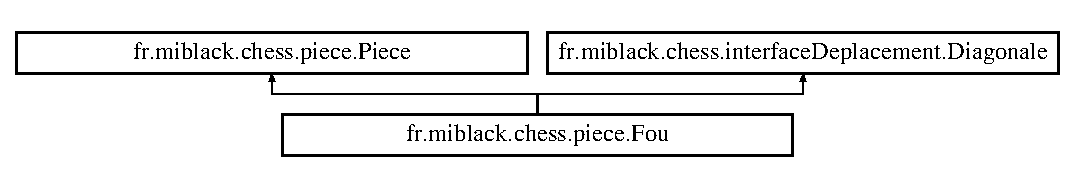
\includegraphics[height=1.866667cm]{classfr_1_1miblack_1_1chess_1_1piece_1_1Fou}
\end{center}
\end{figure}
\subsection*{Public Member Functions}
\begin{DoxyCompactItemize}
\item 
{\bf Fou} ({\bf Couleur} {\bf color}, {\bf Position} {\bf pos}, int {\bf valeur})
\item 
Linked\-List$<$ {\bf Position} $>$ {\bf position\-Accessible} ()
\item 
Linked\-List$<$ {\bf Position} $>$ {\bf position\-Diagonale} ()
\item 
Linked\-List$<$ {\bf Position} $>$ {\bf position\-Accessible\-Chessboard} ({\bf Echiquier} chess)
\item 
Linked\-List$<$ {\bf Position} $>$ {\bf diagonale\-Drt} (int a, {\bf Echiquier} chess)
\item 
Linked\-List$<$ {\bf Position} $>$ {\bf diagonale\-Gch} (int a, {\bf Echiquier} chess)
\item 
Linked\-List$<$ {\bf Position} $>$ {\bf what\-Can\-I\-Eat} ({\bf Echiquier} chess)
\item 
String {\bf to\-String} ()
\item 
String {\bf get\-Nom} ()
\item 
{\bf Piece} {\bf clone} ()
\end{DoxyCompactItemize}
\subsection*{Additional Inherited Members}


\subsection{Detailed Description}
\begin{DoxyAuthor}{Author}
mi-\/black 
\end{DoxyAuthor}


\subsection{Constructor \& Destructor Documentation}
\index{fr\-::miblack\-::chess\-::piece\-::\-Fou@{fr\-::miblack\-::chess\-::piece\-::\-Fou}!Fou@{Fou}}
\index{Fou@{Fou}!fr::miblack::chess::piece::Fou@{fr\-::miblack\-::chess\-::piece\-::\-Fou}}
\subsubsection[{Fou}]{\setlength{\rightskip}{0pt plus 5cm}fr.\-miblack.\-chess.\-piece.\-Fou.\-Fou (
\begin{DoxyParamCaption}
\item[{{\bf Couleur}}]{color, }
\item[{{\bf Position}}]{pos, }
\item[{int}]{valeur}
\end{DoxyParamCaption}
)}\label{classfr_1_1miblack_1_1chess_1_1piece_1_1Fou_a954a3530807e90afb4ebdd03a36b4786}

\begin{DoxyParams}{Parameters}
{\em color} & \\
\hline
{\em pos} & \\
\hline
{\em valeur} & \\
\hline
\end{DoxyParams}


\subsection{Member Function Documentation}
\index{fr\-::miblack\-::chess\-::piece\-::\-Fou@{fr\-::miblack\-::chess\-::piece\-::\-Fou}!clone@{clone}}
\index{clone@{clone}!fr::miblack::chess::piece::Fou@{fr\-::miblack\-::chess\-::piece\-::\-Fou}}
\subsubsection[{clone}]{\setlength{\rightskip}{0pt plus 5cm}{\bf Piece} fr.\-miblack.\-chess.\-piece.\-Fou.\-clone (
\begin{DoxyParamCaption}
{}
\end{DoxyParamCaption}
)}\label{classfr_1_1miblack_1_1chess_1_1piece_1_1Fou_aa1a2cbd08673cd967feb9c17e5cc2bad}
\begin{DoxyReturn}{Returns}

\end{DoxyReturn}
\index{fr\-::miblack\-::chess\-::piece\-::\-Fou@{fr\-::miblack\-::chess\-::piece\-::\-Fou}!diagonale\-Drt@{diagonale\-Drt}}
\index{diagonale\-Drt@{diagonale\-Drt}!fr::miblack::chess::piece::Fou@{fr\-::miblack\-::chess\-::piece\-::\-Fou}}
\subsubsection[{diagonale\-Drt}]{\setlength{\rightskip}{0pt plus 5cm}Linked\-List$<${\bf Position}$>$ fr.\-miblack.\-chess.\-piece.\-Fou.\-diagonale\-Drt (
\begin{DoxyParamCaption}
\item[{int}]{a, }
\item[{{\bf Echiquier}}]{chess}
\end{DoxyParamCaption}
)}\label{classfr_1_1miblack_1_1chess_1_1piece_1_1Fou_af4e8e9ff36c3f45091a9085b9c1715c3}

\begin{DoxyParams}{Parameters}
{\em a} & au dessus ou au dessous \\
\hline
{\em chess} & \\
\hline
\end{DoxyParams}
\begin{DoxyReturn}{Returns}

\end{DoxyReturn}
\index{fr\-::miblack\-::chess\-::piece\-::\-Fou@{fr\-::miblack\-::chess\-::piece\-::\-Fou}!diagonale\-Gch@{diagonale\-Gch}}
\index{diagonale\-Gch@{diagonale\-Gch}!fr::miblack::chess::piece::Fou@{fr\-::miblack\-::chess\-::piece\-::\-Fou}}
\subsubsection[{diagonale\-Gch}]{\setlength{\rightskip}{0pt plus 5cm}Linked\-List$<${\bf Position}$>$ fr.\-miblack.\-chess.\-piece.\-Fou.\-diagonale\-Gch (
\begin{DoxyParamCaption}
\item[{int}]{a, }
\item[{{\bf Echiquier}}]{chess}
\end{DoxyParamCaption}
)}\label{classfr_1_1miblack_1_1chess_1_1piece_1_1Fou_ac8f088baaae744a48d6452284497ce6b}

\begin{DoxyParams}{Parameters}
{\em a} & au dessus ou au dessous \\
\hline
{\em chess} & \\
\hline
\end{DoxyParams}
\begin{DoxyReturn}{Returns}

\end{DoxyReturn}
\index{fr\-::miblack\-::chess\-::piece\-::\-Fou@{fr\-::miblack\-::chess\-::piece\-::\-Fou}!get\-Nom@{get\-Nom}}
\index{get\-Nom@{get\-Nom}!fr::miblack::chess::piece::Fou@{fr\-::miblack\-::chess\-::piece\-::\-Fou}}
\subsubsection[{get\-Nom}]{\setlength{\rightskip}{0pt plus 5cm}String fr.\-miblack.\-chess.\-piece.\-Fou.\-get\-Nom (
\begin{DoxyParamCaption}
{}
\end{DoxyParamCaption}
)}\label{classfr_1_1miblack_1_1chess_1_1piece_1_1Fou_ab925ec7e8e1e1765b9068ecd316f8018}
\begin{DoxyReturn}{Returns}

\end{DoxyReturn}


Reimplemented from {\bf fr.\-miblack.\-chess.\-piece.\-Piece} \doxyref{}{p.}{classfr_1_1miblack_1_1chess_1_1piece_1_1Piece_a68bb44429e21b7f64511a91a0861dde4}.

\index{fr\-::miblack\-::chess\-::piece\-::\-Fou@{fr\-::miblack\-::chess\-::piece\-::\-Fou}!position\-Accessible@{position\-Accessible}}
\index{position\-Accessible@{position\-Accessible}!fr::miblack::chess::piece::Fou@{fr\-::miblack\-::chess\-::piece\-::\-Fou}}
\subsubsection[{position\-Accessible}]{\setlength{\rightskip}{0pt plus 5cm}Linked\-List$<${\bf Position}$>$ fr.\-miblack.\-chess.\-piece.\-Fou.\-position\-Accessible (
\begin{DoxyParamCaption}
{}
\end{DoxyParamCaption}
)\hspace{0.3cm}{\ttfamily [virtual]}}\label{classfr_1_1miblack_1_1chess_1_1piece_1_1Fou_ad3e65280fc7f9bfba09054f2a12acb34}
\begin{DoxyReturn}{Returns}
List of position where one piece can be going 
\end{DoxyReturn}


Implements {\bf fr.\-miblack.\-chess.\-piece.\-Piece} \doxyref{}{p.}{classfr_1_1miblack_1_1chess_1_1piece_1_1Piece_ad5cdbd635ec706f16d57dccf1b8c456e}.

\index{fr\-::miblack\-::chess\-::piece\-::\-Fou@{fr\-::miblack\-::chess\-::piece\-::\-Fou}!position\-Accessible\-Chessboard@{position\-Accessible\-Chessboard}}
\index{position\-Accessible\-Chessboard@{position\-Accessible\-Chessboard}!fr::miblack::chess::piece::Fou@{fr\-::miblack\-::chess\-::piece\-::\-Fou}}
\subsubsection[{position\-Accessible\-Chessboard}]{\setlength{\rightskip}{0pt plus 5cm}Linked\-List$<${\bf Position}$>$ fr.\-miblack.\-chess.\-piece.\-Fou.\-position\-Accessible\-Chessboard (
\begin{DoxyParamCaption}
\item[{{\bf Echiquier}}]{chess}
\end{DoxyParamCaption}
)\hspace{0.3cm}{\ttfamily [virtual]}}\label{classfr_1_1miblack_1_1chess_1_1piece_1_1Fou_a9cdc9221f86c92871cb8ff54ec13843c}
\begin{DoxyReturn}{Returns}
List of position where one piece can be going with restriction of the chessboard 
\end{DoxyReturn}


Implements {\bf fr.\-miblack.\-chess.\-piece.\-Piece} \doxyref{}{p.}{classfr_1_1miblack_1_1chess_1_1piece_1_1Piece_ac1222bad9bf13533eecec2b8d99e24c6}.

\index{fr\-::miblack\-::chess\-::piece\-::\-Fou@{fr\-::miblack\-::chess\-::piece\-::\-Fou}!position\-Diagonale@{position\-Diagonale}}
\index{position\-Diagonale@{position\-Diagonale}!fr::miblack::chess::piece::Fou@{fr\-::miblack\-::chess\-::piece\-::\-Fou}}
\subsubsection[{position\-Diagonale}]{\setlength{\rightskip}{0pt plus 5cm}Linked\-List$<${\bf Position}$>$ fr.\-miblack.\-chess.\-piece.\-Fou.\-position\-Diagonale (
\begin{DoxyParamCaption}
{}
\end{DoxyParamCaption}
)}\label{classfr_1_1miblack_1_1chess_1_1piece_1_1Fou_a60217f99d2d3569644351f9778761c54}
\begin{DoxyReturn}{Returns}
liste des pos diagonales 
\end{DoxyReturn}


Implements {\bf fr.\-miblack.\-chess.\-interface\-Deplacement.\-Diagonale} \doxyref{}{p.}{interfacefr_1_1miblack_1_1chess_1_1interfaceDeplacement_1_1Diagonale_a4d6e3ca777cea05ea561875497ac1161}.

\index{fr\-::miblack\-::chess\-::piece\-::\-Fou@{fr\-::miblack\-::chess\-::piece\-::\-Fou}!to\-String@{to\-String}}
\index{to\-String@{to\-String}!fr::miblack::chess::piece::Fou@{fr\-::miblack\-::chess\-::piece\-::\-Fou}}
\subsubsection[{to\-String}]{\setlength{\rightskip}{0pt plus 5cm}String fr.\-miblack.\-chess.\-piece.\-Fou.\-to\-String (
\begin{DoxyParamCaption}
{}
\end{DoxyParamCaption}
)}\label{classfr_1_1miblack_1_1chess_1_1piece_1_1Fou_a5707a9f1f39ffb397251df634dbb8bbc}
\begin{DoxyReturn}{Returns}

\end{DoxyReturn}
\index{fr\-::miblack\-::chess\-::piece\-::\-Fou@{fr\-::miblack\-::chess\-::piece\-::\-Fou}!what\-Can\-I\-Eat@{what\-Can\-I\-Eat}}
\index{what\-Can\-I\-Eat@{what\-Can\-I\-Eat}!fr::miblack::chess::piece::Fou@{fr\-::miblack\-::chess\-::piece\-::\-Fou}}
\subsubsection[{what\-Can\-I\-Eat}]{\setlength{\rightskip}{0pt plus 5cm}Linked\-List$<${\bf Position}$>$ fr.\-miblack.\-chess.\-piece.\-Fou.\-what\-Can\-I\-Eat (
\begin{DoxyParamCaption}
\item[{{\bf Echiquier}}]{chess}
\end{DoxyParamCaption}
)\hspace{0.3cm}{\ttfamily [virtual]}}\label{classfr_1_1miblack_1_1chess_1_1piece_1_1Fou_a1eb6e0151e98bc2b95eb0150167f9404}

\begin{DoxyParams}{Parameters}
{\em chess} & l'echiquier \\
\hline
\end{DoxyParams}
\begin{DoxyReturn}{Returns}
Liste des position capturables 
\end{DoxyReturn}


Implements {\bf fr.\-miblack.\-chess.\-piece.\-Piece} \doxyref{}{p.}{classfr_1_1miblack_1_1chess_1_1piece_1_1Piece_af18b3bc007e0e50740de39142a5b2919}.



The documentation for this class was generated from the following file\-:\begin{DoxyCompactItemize}
\item 
fr/miblack/chess/piece/Fou.\-java\end{DoxyCompactItemize}

\section{fr.\-miblack.\-chess.\-affichage.\-Graphique Class Reference}
\label{classfr_1_1miblack_1_1chess_1_1affichage_1_1Graphique}\index{fr.\-miblack.\-chess.\-affichage.\-Graphique@{fr.\-miblack.\-chess.\-affichage.\-Graphique}}


Inheritance diagram for fr.\-miblack.\-chess.\-affichage.\-Graphique\-:
\nopagebreak
\begin{figure}[H]
\begin{center}
\leavevmode
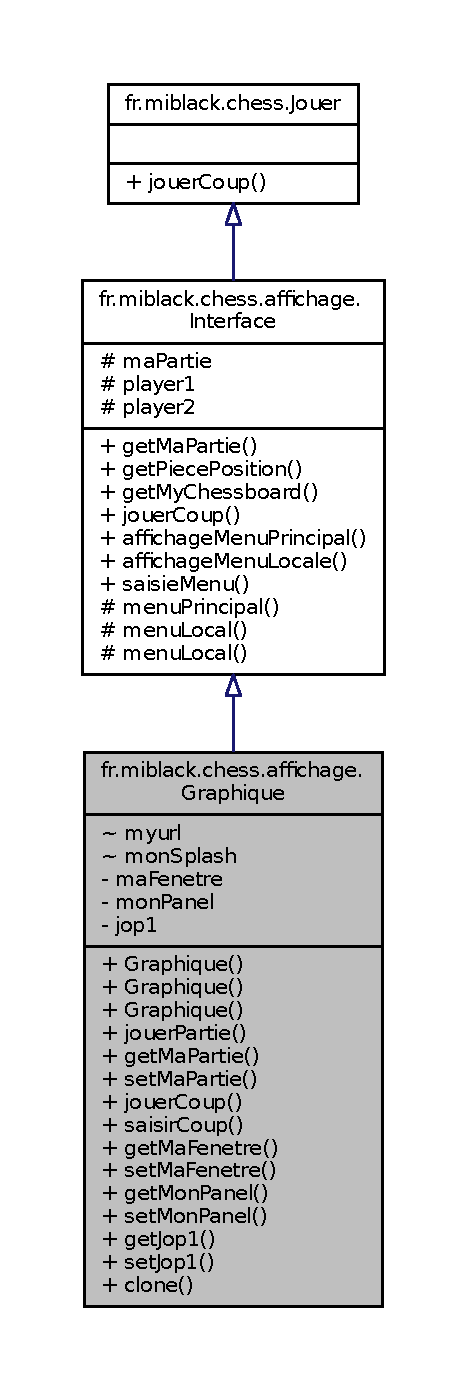
\includegraphics[height=550pt]{classfr_1_1miblack_1_1chess_1_1affichage_1_1Graphique__inherit__graph}
\end{center}
\end{figure}


Collaboration diagram for fr.\-miblack.\-chess.\-affichage.\-Graphique\-:
\nopagebreak
\begin{figure}[H]
\begin{center}
\leavevmode
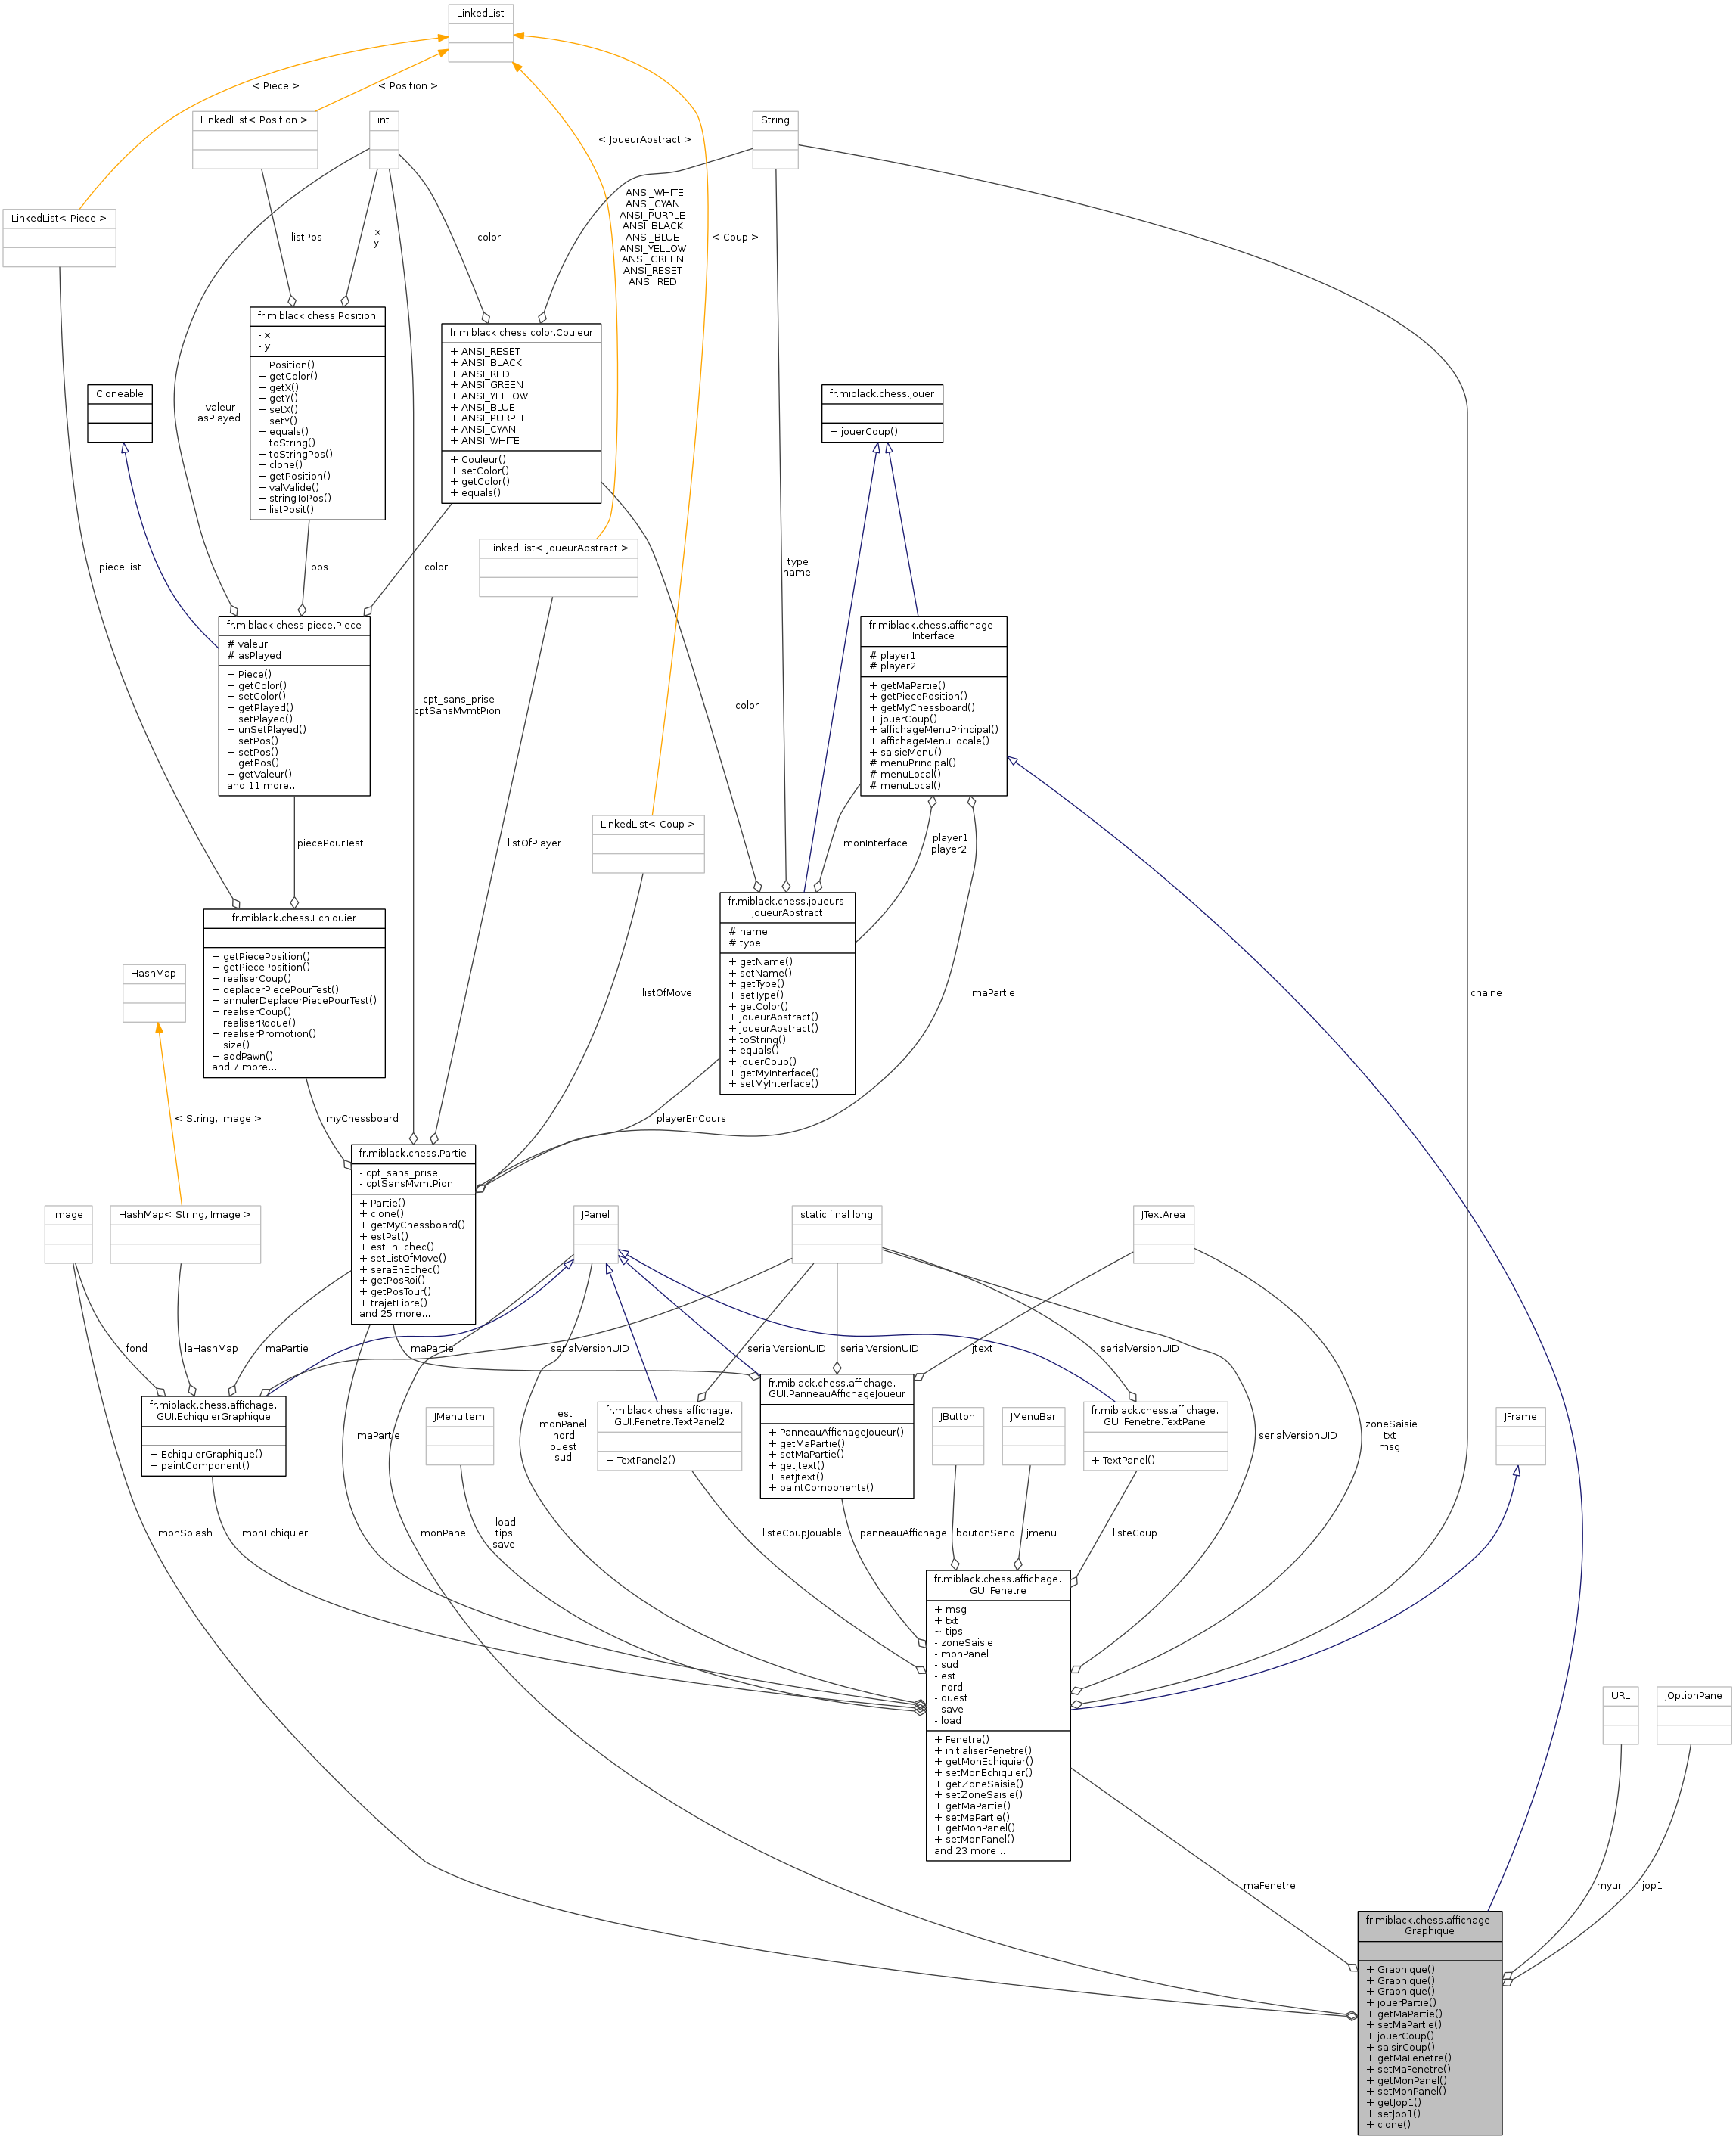
\includegraphics[width=350pt]{classfr_1_1miblack_1_1chess_1_1affichage_1_1Graphique__coll__graph}
\end{center}
\end{figure}
\subsection*{Public Member Functions}
\begin{DoxyCompactItemize}
\item 
{\bf Graphique} (String p1, String p2)
\item 
{\bf Graphique} ()
\item 
{\bf Graphique} ({\bf Partie} partie)
\item 
void {\bf jouer\-Partie} ()
\item 
{\bf Partie} {\bf get\-Ma\-Partie} ()
\item 
void {\bf set\-Ma\-Partie} ({\bf Partie} {\bf ma\-Partie})
\item 
{\bf Coup} {\bf jouer\-Coup} ({\bf Partie} g)
\item 
{\bf Coup} {\bf saisir\-Coup} ({\bf Joueur\-Abstract} p, {\bf Echiquier} chess)
\item 
{\bf Fenetre} {\bf get\-Ma\-Fenetre} ()
\item 
void {\bf set\-Ma\-Fenetre} ({\bf Fenetre} {\bf ma\-Fenetre})
\item 
J\-Panel {\bf get\-Mon\-Panel} ()
\item 
void {\bf set\-Mon\-Panel} (J\-Panel {\bf mon\-Panel})
\item 
J\-Option\-Pane {\bf get\-Jop1} ()
\item 
void {\bf set\-Jop1} (J\-Option\-Pane {\bf jop1})
\item 
{\bf Graphique} {\bf clone} ()
\end{DoxyCompactItemize}
\subsection*{Private Attributes}
\begin{DoxyCompactItemize}
\item 
{\bf Fenetre} {\bf ma\-Fenetre} = null
\item 
J\-Panel {\bf mon\-Panel}
\item 
J\-Option\-Pane {\bf jop1} = new J\-Option\-Pane()
\end{DoxyCompactItemize}
\subsection*{Additional Inherited Members}


\subsection{Detailed Description}
\begin{DoxyAuthor}{Author}
mi-\/black 
\end{DoxyAuthor}


\subsection{Constructor \& Destructor Documentation}
\index{fr\-::miblack\-::chess\-::affichage\-::\-Graphique@{fr\-::miblack\-::chess\-::affichage\-::\-Graphique}!Graphique@{Graphique}}
\index{Graphique@{Graphique}!fr::miblack::chess::affichage::Graphique@{fr\-::miblack\-::chess\-::affichage\-::\-Graphique}}
\subsubsection[{Graphique}]{\setlength{\rightskip}{0pt plus 5cm}fr.\-miblack.\-chess.\-affichage.\-Graphique.\-Graphique (
\begin{DoxyParamCaption}
\item[{String}]{p1, }
\item[{String}]{p2}
\end{DoxyParamCaption}
)}\label{classfr_1_1miblack_1_1chess_1_1affichage_1_1Graphique_a7c4c1ff58265f1fce39c6180318c50fa}

\begin{DoxyParams}{Parameters}
{\em p1} & joueur 1 \\
\hline
{\em p2} & joueur 2 \\
\hline
\end{DoxyParams}
\index{fr\-::miblack\-::chess\-::affichage\-::\-Graphique@{fr\-::miblack\-::chess\-::affichage\-::\-Graphique}!Graphique@{Graphique}}
\index{Graphique@{Graphique}!fr::miblack::chess::affichage::Graphique@{fr\-::miblack\-::chess\-::affichage\-::\-Graphique}}
\subsubsection[{Graphique}]{\setlength{\rightskip}{0pt plus 5cm}fr.\-miblack.\-chess.\-affichage.\-Graphique.\-Graphique (
\begin{DoxyParamCaption}
{}
\end{DoxyParamCaption}
)}\label{classfr_1_1miblack_1_1chess_1_1affichage_1_1Graphique_a0a3fd2ece21cbea942ccefec3289cd08}
\index{fr\-::miblack\-::chess\-::affichage\-::\-Graphique@{fr\-::miblack\-::chess\-::affichage\-::\-Graphique}!Graphique@{Graphique}}
\index{Graphique@{Graphique}!fr::miblack::chess::affichage::Graphique@{fr\-::miblack\-::chess\-::affichage\-::\-Graphique}}
\subsubsection[{Graphique}]{\setlength{\rightskip}{0pt plus 5cm}fr.\-miblack.\-chess.\-affichage.\-Graphique.\-Graphique (
\begin{DoxyParamCaption}
\item[{{\bf Partie}}]{partie}
\end{DoxyParamCaption}
)}\label{classfr_1_1miblack_1_1chess_1_1affichage_1_1Graphique_ada6ab555f4c959d50f45b461a8b3310f}

\begin{DoxyParams}{Parameters}
{\em partie} & \\
\hline
\end{DoxyParams}


\subsection{Member Function Documentation}
\index{fr\-::miblack\-::chess\-::affichage\-::\-Graphique@{fr\-::miblack\-::chess\-::affichage\-::\-Graphique}!clone@{clone}}
\index{clone@{clone}!fr::miblack::chess::affichage::Graphique@{fr\-::miblack\-::chess\-::affichage\-::\-Graphique}}
\subsubsection[{clone}]{\setlength{\rightskip}{0pt plus 5cm}{\bf Graphique} fr.\-miblack.\-chess.\-affichage.\-Graphique.\-clone (
\begin{DoxyParamCaption}
{}
\end{DoxyParamCaption}
)}\label{classfr_1_1miblack_1_1chess_1_1affichage_1_1Graphique_ab9f66c475c0f0c887cdf574e3e834c3d}
\begin{DoxyReturn}{Returns}

\end{DoxyReturn}
\index{fr\-::miblack\-::chess\-::affichage\-::\-Graphique@{fr\-::miblack\-::chess\-::affichage\-::\-Graphique}!get\-Jop1@{get\-Jop1}}
\index{get\-Jop1@{get\-Jop1}!fr::miblack::chess::affichage::Graphique@{fr\-::miblack\-::chess\-::affichage\-::\-Graphique}}
\subsubsection[{get\-Jop1}]{\setlength{\rightskip}{0pt plus 5cm}J\-Option\-Pane fr.\-miblack.\-chess.\-affichage.\-Graphique.\-get\-Jop1 (
\begin{DoxyParamCaption}
{}
\end{DoxyParamCaption}
)}\label{classfr_1_1miblack_1_1chess_1_1affichage_1_1Graphique_a9c088a7f6fd51e6d64fe3385e1970dd2}
\begin{DoxyReturn}{Returns}

\end{DoxyReturn}
\index{fr\-::miblack\-::chess\-::affichage\-::\-Graphique@{fr\-::miblack\-::chess\-::affichage\-::\-Graphique}!get\-Ma\-Fenetre@{get\-Ma\-Fenetre}}
\index{get\-Ma\-Fenetre@{get\-Ma\-Fenetre}!fr::miblack::chess::affichage::Graphique@{fr\-::miblack\-::chess\-::affichage\-::\-Graphique}}
\subsubsection[{get\-Ma\-Fenetre}]{\setlength{\rightskip}{0pt plus 5cm}{\bf Fenetre} fr.\-miblack.\-chess.\-affichage.\-Graphique.\-get\-Ma\-Fenetre (
\begin{DoxyParamCaption}
{}
\end{DoxyParamCaption}
)}\label{classfr_1_1miblack_1_1chess_1_1affichage_1_1Graphique_aea8bb31b6ec953bbeb59b4aed0cbca1d}
\begin{DoxyReturn}{Returns}

\end{DoxyReturn}
\index{fr\-::miblack\-::chess\-::affichage\-::\-Graphique@{fr\-::miblack\-::chess\-::affichage\-::\-Graphique}!get\-Ma\-Partie@{get\-Ma\-Partie}}
\index{get\-Ma\-Partie@{get\-Ma\-Partie}!fr::miblack::chess::affichage::Graphique@{fr\-::miblack\-::chess\-::affichage\-::\-Graphique}}
\subsubsection[{get\-Ma\-Partie}]{\setlength{\rightskip}{0pt plus 5cm}{\bf Partie} fr.\-miblack.\-chess.\-affichage.\-Graphique.\-get\-Ma\-Partie (
\begin{DoxyParamCaption}
{}
\end{DoxyParamCaption}
)}\label{classfr_1_1miblack_1_1chess_1_1affichage_1_1Graphique_ad486b51985e261e3f6332046889f2484}
\begin{DoxyReturn}{Returns}

\end{DoxyReturn}


Reimplemented from {\bf fr.\-miblack.\-chess.\-affichage.\-Interface} \doxyref{}{p.}{classfr_1_1miblack_1_1chess_1_1affichage_1_1Interface_a0157ac3458c0a9ddc490a6d8dffc21cf}.

\index{fr\-::miblack\-::chess\-::affichage\-::\-Graphique@{fr\-::miblack\-::chess\-::affichage\-::\-Graphique}!get\-Mon\-Panel@{get\-Mon\-Panel}}
\index{get\-Mon\-Panel@{get\-Mon\-Panel}!fr::miblack::chess::affichage::Graphique@{fr\-::miblack\-::chess\-::affichage\-::\-Graphique}}
\subsubsection[{get\-Mon\-Panel}]{\setlength{\rightskip}{0pt plus 5cm}J\-Panel fr.\-miblack.\-chess.\-affichage.\-Graphique.\-get\-Mon\-Panel (
\begin{DoxyParamCaption}
{}
\end{DoxyParamCaption}
)}\label{classfr_1_1miblack_1_1chess_1_1affichage_1_1Graphique_aeff4487f382f17dbee5e2ed2a94c4e8e}
\begin{DoxyReturn}{Returns}

\end{DoxyReturn}
\index{fr\-::miblack\-::chess\-::affichage\-::\-Graphique@{fr\-::miblack\-::chess\-::affichage\-::\-Graphique}!jouer\-Coup@{jouer\-Coup}}
\index{jouer\-Coup@{jouer\-Coup}!fr::miblack::chess::affichage::Graphique@{fr\-::miblack\-::chess\-::affichage\-::\-Graphique}}
\subsubsection[{jouer\-Coup}]{\setlength{\rightskip}{0pt plus 5cm}{\bf Coup} fr.\-miblack.\-chess.\-affichage.\-Graphique.\-jouer\-Coup (
\begin{DoxyParamCaption}
\item[{{\bf Partie}}]{g}
\end{DoxyParamCaption}
)\hspace{0.3cm}{\ttfamily [virtual]}}\label{classfr_1_1miblack_1_1chess_1_1affichage_1_1Graphique_aa614e0e0e7cce0dac59276b59b04a549}

\begin{DoxyParams}{Parameters}
{\em g} & une partie \\
\hline
\end{DoxyParams}
\begin{DoxyReturn}{Returns}
le coup Joué 
\end{DoxyReturn}


Implements {\bf fr.\-miblack.\-chess.\-affichage.\-Interface} \doxyref{}{p.}{classfr_1_1miblack_1_1chess_1_1affichage_1_1Interface_a16a7abd6c521cb1e9cdafb5f586db68b}.

\index{fr\-::miblack\-::chess\-::affichage\-::\-Graphique@{fr\-::miblack\-::chess\-::affichage\-::\-Graphique}!jouer\-Partie@{jouer\-Partie}}
\index{jouer\-Partie@{jouer\-Partie}!fr::miblack::chess::affichage::Graphique@{fr\-::miblack\-::chess\-::affichage\-::\-Graphique}}
\subsubsection[{jouer\-Partie}]{\setlength{\rightskip}{0pt plus 5cm}void fr.\-miblack.\-chess.\-affichage.\-Graphique.\-jouer\-Partie (
\begin{DoxyParamCaption}
{}
\end{DoxyParamCaption}
)}\label{classfr_1_1miblack_1_1chess_1_1affichage_1_1Graphique_a7e81889ee5ce6dbe1efce754a5c53405}
déroulement de la partie en \doxyref{G\-U\-I}{p.}{namespacefr_1_1miblack_1_1chess_1_1affichage_1_1GUI} \index{fr\-::miblack\-::chess\-::affichage\-::\-Graphique@{fr\-::miblack\-::chess\-::affichage\-::\-Graphique}!saisir\-Coup@{saisir\-Coup}}
\index{saisir\-Coup@{saisir\-Coup}!fr::miblack::chess::affichage::Graphique@{fr\-::miblack\-::chess\-::affichage\-::\-Graphique}}
\subsubsection[{saisir\-Coup}]{\setlength{\rightskip}{0pt plus 5cm}{\bf Coup} fr.\-miblack.\-chess.\-affichage.\-Graphique.\-saisir\-Coup (
\begin{DoxyParamCaption}
\item[{{\bf Joueur\-Abstract}}]{p, }
\item[{{\bf Echiquier}}]{chess}
\end{DoxyParamCaption}
)}\label{classfr_1_1miblack_1_1chess_1_1affichage_1_1Graphique_ad5019e7ee32fb547f98ff4f6d73ce26b}

\begin{DoxyParams}{Parameters}
{\em p} & le joueur \\
\hline
{\em chess} & l'echiquier \\
\hline
\end{DoxyParams}
\begin{DoxyReturn}{Returns}
le coup saisi 
\end{DoxyReturn}
\index{fr\-::miblack\-::chess\-::affichage\-::\-Graphique@{fr\-::miblack\-::chess\-::affichage\-::\-Graphique}!set\-Jop1@{set\-Jop1}}
\index{set\-Jop1@{set\-Jop1}!fr::miblack::chess::affichage::Graphique@{fr\-::miblack\-::chess\-::affichage\-::\-Graphique}}
\subsubsection[{set\-Jop1}]{\setlength{\rightskip}{0pt plus 5cm}void fr.\-miblack.\-chess.\-affichage.\-Graphique.\-set\-Jop1 (
\begin{DoxyParamCaption}
\item[{J\-Option\-Pane}]{jop1}
\end{DoxyParamCaption}
)}\label{classfr_1_1miblack_1_1chess_1_1affichage_1_1Graphique_a6e27c05292512a693cbff9c65fdcadfe}

\begin{DoxyParams}{Parameters}
{\em jop1} & \\
\hline
\end{DoxyParams}
\index{fr\-::miblack\-::chess\-::affichage\-::\-Graphique@{fr\-::miblack\-::chess\-::affichage\-::\-Graphique}!set\-Ma\-Fenetre@{set\-Ma\-Fenetre}}
\index{set\-Ma\-Fenetre@{set\-Ma\-Fenetre}!fr::miblack::chess::affichage::Graphique@{fr\-::miblack\-::chess\-::affichage\-::\-Graphique}}
\subsubsection[{set\-Ma\-Fenetre}]{\setlength{\rightskip}{0pt plus 5cm}void fr.\-miblack.\-chess.\-affichage.\-Graphique.\-set\-Ma\-Fenetre (
\begin{DoxyParamCaption}
\item[{{\bf Fenetre}}]{ma\-Fenetre}
\end{DoxyParamCaption}
)}\label{classfr_1_1miblack_1_1chess_1_1affichage_1_1Graphique_a7a7ed666d8726a22794949c1dabc46bc}

\begin{DoxyParams}{Parameters}
{\em ma\-Fenetre} & \\
\hline
\end{DoxyParams}
\index{fr\-::miblack\-::chess\-::affichage\-::\-Graphique@{fr\-::miblack\-::chess\-::affichage\-::\-Graphique}!set\-Ma\-Partie@{set\-Ma\-Partie}}
\index{set\-Ma\-Partie@{set\-Ma\-Partie}!fr::miblack::chess::affichage::Graphique@{fr\-::miblack\-::chess\-::affichage\-::\-Graphique}}
\subsubsection[{set\-Ma\-Partie}]{\setlength{\rightskip}{0pt plus 5cm}void fr.\-miblack.\-chess.\-affichage.\-Graphique.\-set\-Ma\-Partie (
\begin{DoxyParamCaption}
\item[{{\bf Partie}}]{ma\-Partie}
\end{DoxyParamCaption}
)}\label{classfr_1_1miblack_1_1chess_1_1affichage_1_1Graphique_a310b3ac4ab8886e3ca4c0476ebd8ab24}

\begin{DoxyParams}{Parameters}
{\em ma\-Partie} & \\
\hline
\end{DoxyParams}
\index{fr\-::miblack\-::chess\-::affichage\-::\-Graphique@{fr\-::miblack\-::chess\-::affichage\-::\-Graphique}!set\-Mon\-Panel@{set\-Mon\-Panel}}
\index{set\-Mon\-Panel@{set\-Mon\-Panel}!fr::miblack::chess::affichage::Graphique@{fr\-::miblack\-::chess\-::affichage\-::\-Graphique}}
\subsubsection[{set\-Mon\-Panel}]{\setlength{\rightskip}{0pt plus 5cm}void fr.\-miblack.\-chess.\-affichage.\-Graphique.\-set\-Mon\-Panel (
\begin{DoxyParamCaption}
\item[{J\-Panel}]{mon\-Panel}
\end{DoxyParamCaption}
)}\label{classfr_1_1miblack_1_1chess_1_1affichage_1_1Graphique_a8be657548cb806864f683b4c2c760765}

\begin{DoxyParams}{Parameters}
{\em mon\-Panel} & \\
\hline
\end{DoxyParams}


\subsection{Member Data Documentation}
\index{fr\-::miblack\-::chess\-::affichage\-::\-Graphique@{fr\-::miblack\-::chess\-::affichage\-::\-Graphique}!jop1@{jop1}}
\index{jop1@{jop1}!fr::miblack::chess::affichage::Graphique@{fr\-::miblack\-::chess\-::affichage\-::\-Graphique}}
\subsubsection[{jop1}]{\setlength{\rightskip}{0pt plus 5cm}J\-Option\-Pane fr.\-miblack.\-chess.\-affichage.\-Graphique.\-jop1 = new J\-Option\-Pane()\hspace{0.3cm}{\ttfamily [private]}}\label{classfr_1_1miblack_1_1chess_1_1affichage_1_1Graphique_a84d91b5150a6b46fae744b4a4b143c0f}
\index{fr\-::miblack\-::chess\-::affichage\-::\-Graphique@{fr\-::miblack\-::chess\-::affichage\-::\-Graphique}!ma\-Fenetre@{ma\-Fenetre}}
\index{ma\-Fenetre@{ma\-Fenetre}!fr::miblack::chess::affichage::Graphique@{fr\-::miblack\-::chess\-::affichage\-::\-Graphique}}
\subsubsection[{ma\-Fenetre}]{\setlength{\rightskip}{0pt plus 5cm}{\bf Fenetre} fr.\-miblack.\-chess.\-affichage.\-Graphique.\-ma\-Fenetre = null\hspace{0.3cm}{\ttfamily [private]}}\label{classfr_1_1miblack_1_1chess_1_1affichage_1_1Graphique_a32a63b6c3afbc079f966689d0724b51c}
\index{fr\-::miblack\-::chess\-::affichage\-::\-Graphique@{fr\-::miblack\-::chess\-::affichage\-::\-Graphique}!mon\-Panel@{mon\-Panel}}
\index{mon\-Panel@{mon\-Panel}!fr::miblack::chess::affichage::Graphique@{fr\-::miblack\-::chess\-::affichage\-::\-Graphique}}
\subsubsection[{mon\-Panel}]{\setlength{\rightskip}{0pt plus 5cm}J\-Panel fr.\-miblack.\-chess.\-affichage.\-Graphique.\-mon\-Panel\hspace{0.3cm}{\ttfamily [private]}}\label{classfr_1_1miblack_1_1chess_1_1affichage_1_1Graphique_a76065c1f198f1bfef189bede8fd31867}


The documentation for this class was generated from the following file\-:\begin{DoxyCompactItemize}
\item 
fr/miblack/chess/affichage/{\bf Graphique.\-java}\end{DoxyCompactItemize}

\section{fr.\-miblack.\-chess.\-affichage.\-Interface Class Reference}
\label{classfr_1_1miblack_1_1chess_1_1affichage_1_1Interface}\index{fr.\-miblack.\-chess.\-affichage.\-Interface@{fr.\-miblack.\-chess.\-affichage.\-Interface}}
Inheritance diagram for fr.\-miblack.\-chess.\-affichage.\-Interface\-:\begin{figure}[H]
\begin{center}
\leavevmode
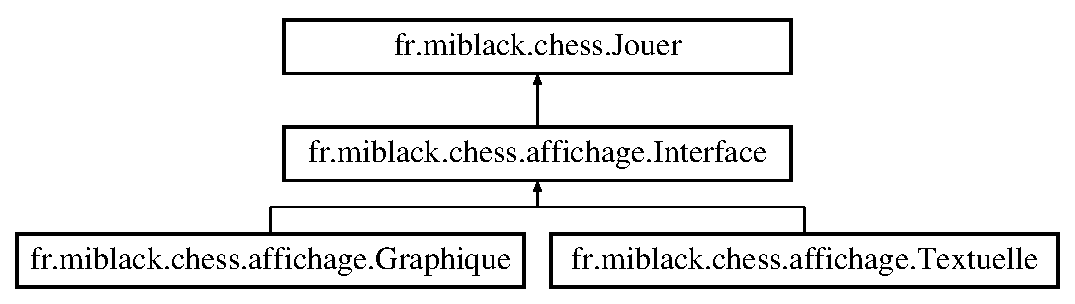
\includegraphics[height=3.000000cm]{classfr_1_1miblack_1_1chess_1_1affichage_1_1Interface}
\end{center}
\end{figure}
\subsection*{Public Member Functions}
\begin{DoxyCompactItemize}
\item 
{\bf Partie} {\bf get\-Ma\-Partie} ()
\item 
{\bf Piece} {\bf get\-Piece\-Position} (int x, int y)
\item 
{\bf Echiquier} {\bf get\-My\-Chessboard} ()
\item 
abstract {\bf Coup} {\bf jouer\-Coup} ({\bf Partie} g)
\item 
int {\bf affichage\-Menu\-Principal} ()
\item 
int {\bf affichage\-Menu\-Locale} ()
\item 
int {\bf saisie\-Menu} (int taille)
\end{DoxyCompactItemize}
\subsection*{Protected Member Functions}
\begin{DoxyCompactItemize}
\item 
void {\bf menu\-Principal} ()
\item 
int {\bf menu\-Local} ()
\item 
int {\bf menu\-Local} (String p1, String p2)
\end{DoxyCompactItemize}
\subsection*{Protected Attributes}
\begin{DoxyCompactItemize}
\item 
{\bf Partie} {\bf ma\-Partie}
\item 
{\bf Joueur\-Abstract} {\bf player1}
\item 
{\bf Joueur\-Abstract} {\bf player2}
\end{DoxyCompactItemize}


\subsection{Detailed Description}
\begin{DoxyAuthor}{Author}
mi-\/black interfaces abstraite 
\end{DoxyAuthor}


\subsection{Member Function Documentation}
\index{fr\-::miblack\-::chess\-::affichage\-::\-Interface@{fr\-::miblack\-::chess\-::affichage\-::\-Interface}!affichage\-Menu\-Locale@{affichage\-Menu\-Locale}}
\index{affichage\-Menu\-Locale@{affichage\-Menu\-Locale}!fr::miblack::chess::affichage::Interface@{fr\-::miblack\-::chess\-::affichage\-::\-Interface}}
\subsubsection[{affichage\-Menu\-Locale}]{\setlength{\rightskip}{0pt plus 5cm}int fr.\-miblack.\-chess.\-affichage.\-Interface.\-affichage\-Menu\-Locale (
\begin{DoxyParamCaption}
{}
\end{DoxyParamCaption}
)}\label{classfr_1_1miblack_1_1chess_1_1affichage_1_1Interface_ab2f65d1ae99227f39ac07af8a679fbf3}
\begin{DoxyReturn}{Returns}

\end{DoxyReturn}
\index{fr\-::miblack\-::chess\-::affichage\-::\-Interface@{fr\-::miblack\-::chess\-::affichage\-::\-Interface}!affichage\-Menu\-Principal@{affichage\-Menu\-Principal}}
\index{affichage\-Menu\-Principal@{affichage\-Menu\-Principal}!fr::miblack::chess::affichage::Interface@{fr\-::miblack\-::chess\-::affichage\-::\-Interface}}
\subsubsection[{affichage\-Menu\-Principal}]{\setlength{\rightskip}{0pt plus 5cm}int fr.\-miblack.\-chess.\-affichage.\-Interface.\-affichage\-Menu\-Principal (
\begin{DoxyParamCaption}
{}
\end{DoxyParamCaption}
)}\label{classfr_1_1miblack_1_1chess_1_1affichage_1_1Interface_a3f1426e093d679166f875a2a4f6dd9dc}
\begin{DoxyReturn}{Returns}

\end{DoxyReturn}
\index{fr\-::miblack\-::chess\-::affichage\-::\-Interface@{fr\-::miblack\-::chess\-::affichage\-::\-Interface}!get\-Ma\-Partie@{get\-Ma\-Partie}}
\index{get\-Ma\-Partie@{get\-Ma\-Partie}!fr::miblack::chess::affichage::Interface@{fr\-::miblack\-::chess\-::affichage\-::\-Interface}}
\subsubsection[{get\-Ma\-Partie}]{\setlength{\rightskip}{0pt plus 5cm}{\bf Partie} fr.\-miblack.\-chess.\-affichage.\-Interface.\-get\-Ma\-Partie (
\begin{DoxyParamCaption}
{}
\end{DoxyParamCaption}
)}\label{classfr_1_1miblack_1_1chess_1_1affichage_1_1Interface_a0157ac3458c0a9ddc490a6d8dffc21cf}
\begin{DoxyReturn}{Returns}

\end{DoxyReturn}


Reimplemented in {\bf fr.\-miblack.\-chess.\-affichage.\-Graphique} \doxyref{}{p.}{classfr_1_1miblack_1_1chess_1_1affichage_1_1Graphique_ad486b51985e261e3f6332046889f2484}.

\index{fr\-::miblack\-::chess\-::affichage\-::\-Interface@{fr\-::miblack\-::chess\-::affichage\-::\-Interface}!get\-My\-Chessboard@{get\-My\-Chessboard}}
\index{get\-My\-Chessboard@{get\-My\-Chessboard}!fr::miblack::chess::affichage::Interface@{fr\-::miblack\-::chess\-::affichage\-::\-Interface}}
\subsubsection[{get\-My\-Chessboard}]{\setlength{\rightskip}{0pt plus 5cm}{\bf Echiquier} fr.\-miblack.\-chess.\-affichage.\-Interface.\-get\-My\-Chessboard (
\begin{DoxyParamCaption}
{}
\end{DoxyParamCaption}
)}\label{classfr_1_1miblack_1_1chess_1_1affichage_1_1Interface_a23fd14bf23379aae5682fbfea7b32bef}
\begin{DoxyReturn}{Returns}

\end{DoxyReturn}
\index{fr\-::miblack\-::chess\-::affichage\-::\-Interface@{fr\-::miblack\-::chess\-::affichage\-::\-Interface}!get\-Piece\-Position@{get\-Piece\-Position}}
\index{get\-Piece\-Position@{get\-Piece\-Position}!fr::miblack::chess::affichage::Interface@{fr\-::miblack\-::chess\-::affichage\-::\-Interface}}
\subsubsection[{get\-Piece\-Position}]{\setlength{\rightskip}{0pt plus 5cm}{\bf Piece} fr.\-miblack.\-chess.\-affichage.\-Interface.\-get\-Piece\-Position (
\begin{DoxyParamCaption}
\item[{int}]{x, }
\item[{int}]{y}
\end{DoxyParamCaption}
)}\label{classfr_1_1miblack_1_1chess_1_1affichage_1_1Interface_aa628b9957428f7a9c8dc3280e7bff15b}

\begin{DoxyParams}{Parameters}
{\em x} & \\
\hline
{\em y} & \\
\hline
\end{DoxyParams}
\begin{DoxyReturn}{Returns}
piece a la position 
\end{DoxyReturn}
\index{fr\-::miblack\-::chess\-::affichage\-::\-Interface@{fr\-::miblack\-::chess\-::affichage\-::\-Interface}!jouer\-Coup@{jouer\-Coup}}
\index{jouer\-Coup@{jouer\-Coup}!fr::miblack::chess::affichage::Interface@{fr\-::miblack\-::chess\-::affichage\-::\-Interface}}
\subsubsection[{jouer\-Coup}]{\setlength{\rightskip}{0pt plus 5cm}abstract {\bf Coup} fr.\-miblack.\-chess.\-affichage.\-Interface.\-jouer\-Coup (
\begin{DoxyParamCaption}
\item[{{\bf Partie}}]{g}
\end{DoxyParamCaption}
)\hspace{0.3cm}{\ttfamily [pure virtual]}}\label{classfr_1_1miblack_1_1chess_1_1affichage_1_1Interface_a16a7abd6c521cb1e9cdafb5f586db68b}

\begin{DoxyParams}{Parameters}
{\em g} & une partie \\
\hline
\end{DoxyParams}
\begin{DoxyReturn}{Returns}
le coup Joué 
\end{DoxyReturn}


Implements {\bf fr.\-miblack.\-chess.\-Jouer} \doxyref{}{p.}{interfacefr_1_1miblack_1_1chess_1_1Jouer_a37f671e9b8707e21e02ea5dfbe83937f}.



Implemented in {\bf fr.\-miblack.\-chess.\-affichage.\-Graphique} \doxyref{}{p.}{classfr_1_1miblack_1_1chess_1_1affichage_1_1Graphique_aa614e0e0e7cce0dac59276b59b04a549}, and {\bf fr.\-miblack.\-chess.\-affichage.\-Textuelle} \doxyref{}{p.}{classfr_1_1miblack_1_1chess_1_1affichage_1_1Textuelle_a2fe98d89987be73eed0e7d666d16f3f5}.

\index{fr\-::miblack\-::chess\-::affichage\-::\-Interface@{fr\-::miblack\-::chess\-::affichage\-::\-Interface}!menu\-Local@{menu\-Local}}
\index{menu\-Local@{menu\-Local}!fr::miblack::chess::affichage::Interface@{fr\-::miblack\-::chess\-::affichage\-::\-Interface}}
\subsubsection[{menu\-Local}]{\setlength{\rightskip}{0pt plus 5cm}int fr.\-miblack.\-chess.\-affichage.\-Interface.\-menu\-Local (
\begin{DoxyParamCaption}
{}
\end{DoxyParamCaption}
)\hspace{0.3cm}{\ttfamily [protected]}}\label{classfr_1_1miblack_1_1chess_1_1affichage_1_1Interface_a3edbf384342b1f4df48cdeb044067abf}
le menu local \index{fr\-::miblack\-::chess\-::affichage\-::\-Interface@{fr\-::miblack\-::chess\-::affichage\-::\-Interface}!menu\-Local@{menu\-Local}}
\index{menu\-Local@{menu\-Local}!fr::miblack::chess::affichage::Interface@{fr\-::miblack\-::chess\-::affichage\-::\-Interface}}
\subsubsection[{menu\-Local}]{\setlength{\rightskip}{0pt plus 5cm}int fr.\-miblack.\-chess.\-affichage.\-Interface.\-menu\-Local (
\begin{DoxyParamCaption}
\item[{String}]{p1, }
\item[{String}]{p2}
\end{DoxyParamCaption}
)\hspace{0.3cm}{\ttfamily [protected]}}\label{classfr_1_1miblack_1_1chess_1_1affichage_1_1Interface_a9eab1d06f27f58534648dfc93e93c58f}

\begin{DoxyParams}{Parameters}
{\em p1} & \\
\hline
{\em p2} & \\
\hline
\end{DoxyParams}
\begin{DoxyReturn}{Returns}

\end{DoxyReturn}
\index{fr\-::miblack\-::chess\-::affichage\-::\-Interface@{fr\-::miblack\-::chess\-::affichage\-::\-Interface}!menu\-Principal@{menu\-Principal}}
\index{menu\-Principal@{menu\-Principal}!fr::miblack::chess::affichage::Interface@{fr\-::miblack\-::chess\-::affichage\-::\-Interface}}
\subsubsection[{menu\-Principal}]{\setlength{\rightskip}{0pt plus 5cm}void fr.\-miblack.\-chess.\-affichage.\-Interface.\-menu\-Principal (
\begin{DoxyParamCaption}
{}
\end{DoxyParamCaption}
)\hspace{0.3cm}{\ttfamily [protected]}}\label{classfr_1_1miblack_1_1chess_1_1affichage_1_1Interface_aacc8fcc7660a3890d6a9e0a3cff2e479}
Affichage menu principal \index{fr\-::miblack\-::chess\-::affichage\-::\-Interface@{fr\-::miblack\-::chess\-::affichage\-::\-Interface}!saisie\-Menu@{saisie\-Menu}}
\index{saisie\-Menu@{saisie\-Menu}!fr::miblack::chess::affichage::Interface@{fr\-::miblack\-::chess\-::affichage\-::\-Interface}}
\subsubsection[{saisie\-Menu}]{\setlength{\rightskip}{0pt plus 5cm}int fr.\-miblack.\-chess.\-affichage.\-Interface.\-saisie\-Menu (
\begin{DoxyParamCaption}
\item[{int}]{taille}
\end{DoxyParamCaption}
)}\label{classfr_1_1miblack_1_1chess_1_1affichage_1_1Interface_a0de3c902bfa4ec8ad859746101c01f8d}

\begin{DoxyParams}{Parameters}
{\em taille} & du menu \\
\hline
\end{DoxyParams}
\begin{DoxyReturn}{Returns}
nbre saisi 
\end{DoxyReturn}


\subsection{Member Data Documentation}
\index{fr\-::miblack\-::chess\-::affichage\-::\-Interface@{fr\-::miblack\-::chess\-::affichage\-::\-Interface}!ma\-Partie@{ma\-Partie}}
\index{ma\-Partie@{ma\-Partie}!fr::miblack::chess::affichage::Interface@{fr\-::miblack\-::chess\-::affichage\-::\-Interface}}
\subsubsection[{ma\-Partie}]{\setlength{\rightskip}{0pt plus 5cm}{\bf Partie} fr.\-miblack.\-chess.\-affichage.\-Interface.\-ma\-Partie\hspace{0.3cm}{\ttfamily [protected]}}\label{classfr_1_1miblack_1_1chess_1_1affichage_1_1Interface_a8b741b2dde887b0ceabeea5b2b39233b}
la partie \index{fr\-::miblack\-::chess\-::affichage\-::\-Interface@{fr\-::miblack\-::chess\-::affichage\-::\-Interface}!player1@{player1}}
\index{player1@{player1}!fr::miblack::chess::affichage::Interface@{fr\-::miblack\-::chess\-::affichage\-::\-Interface}}
\subsubsection[{player1}]{\setlength{\rightskip}{0pt plus 5cm}{\bf Joueur\-Abstract} fr.\-miblack.\-chess.\-affichage.\-Interface.\-player1\hspace{0.3cm}{\ttfamily [protected]}}\label{classfr_1_1miblack_1_1chess_1_1affichage_1_1Interface_a82755dafb79459bb428ff06db523b414}
le j1 \index{fr\-::miblack\-::chess\-::affichage\-::\-Interface@{fr\-::miblack\-::chess\-::affichage\-::\-Interface}!player2@{player2}}
\index{player2@{player2}!fr::miblack::chess::affichage::Interface@{fr\-::miblack\-::chess\-::affichage\-::\-Interface}}
\subsubsection[{player2}]{\setlength{\rightskip}{0pt plus 5cm}{\bf Joueur\-Abstract} fr.\-miblack.\-chess.\-affichage.\-Interface.\-player2\hspace{0.3cm}{\ttfamily [protected]}}\label{classfr_1_1miblack_1_1chess_1_1affichage_1_1Interface_a80ff7115c81896f1021ef764993b9bff}
le j2 

The documentation for this class was generated from the following file\-:\begin{DoxyCompactItemize}
\item 
fr/miblack/chess/affichage/Interface.\-java\end{DoxyCompactItemize}

\section{fr.\-miblack.\-chess.\-Jouer Interface Reference}
\label{interfacefr_1_1miblack_1_1chess_1_1Jouer}\index{fr.\-miblack.\-chess.\-Jouer@{fr.\-miblack.\-chess.\-Jouer}}


Inheritance diagram for fr.\-miblack.\-chess.\-Jouer\-:
\nopagebreak
\begin{figure}[H]
\begin{center}
\leavevmode
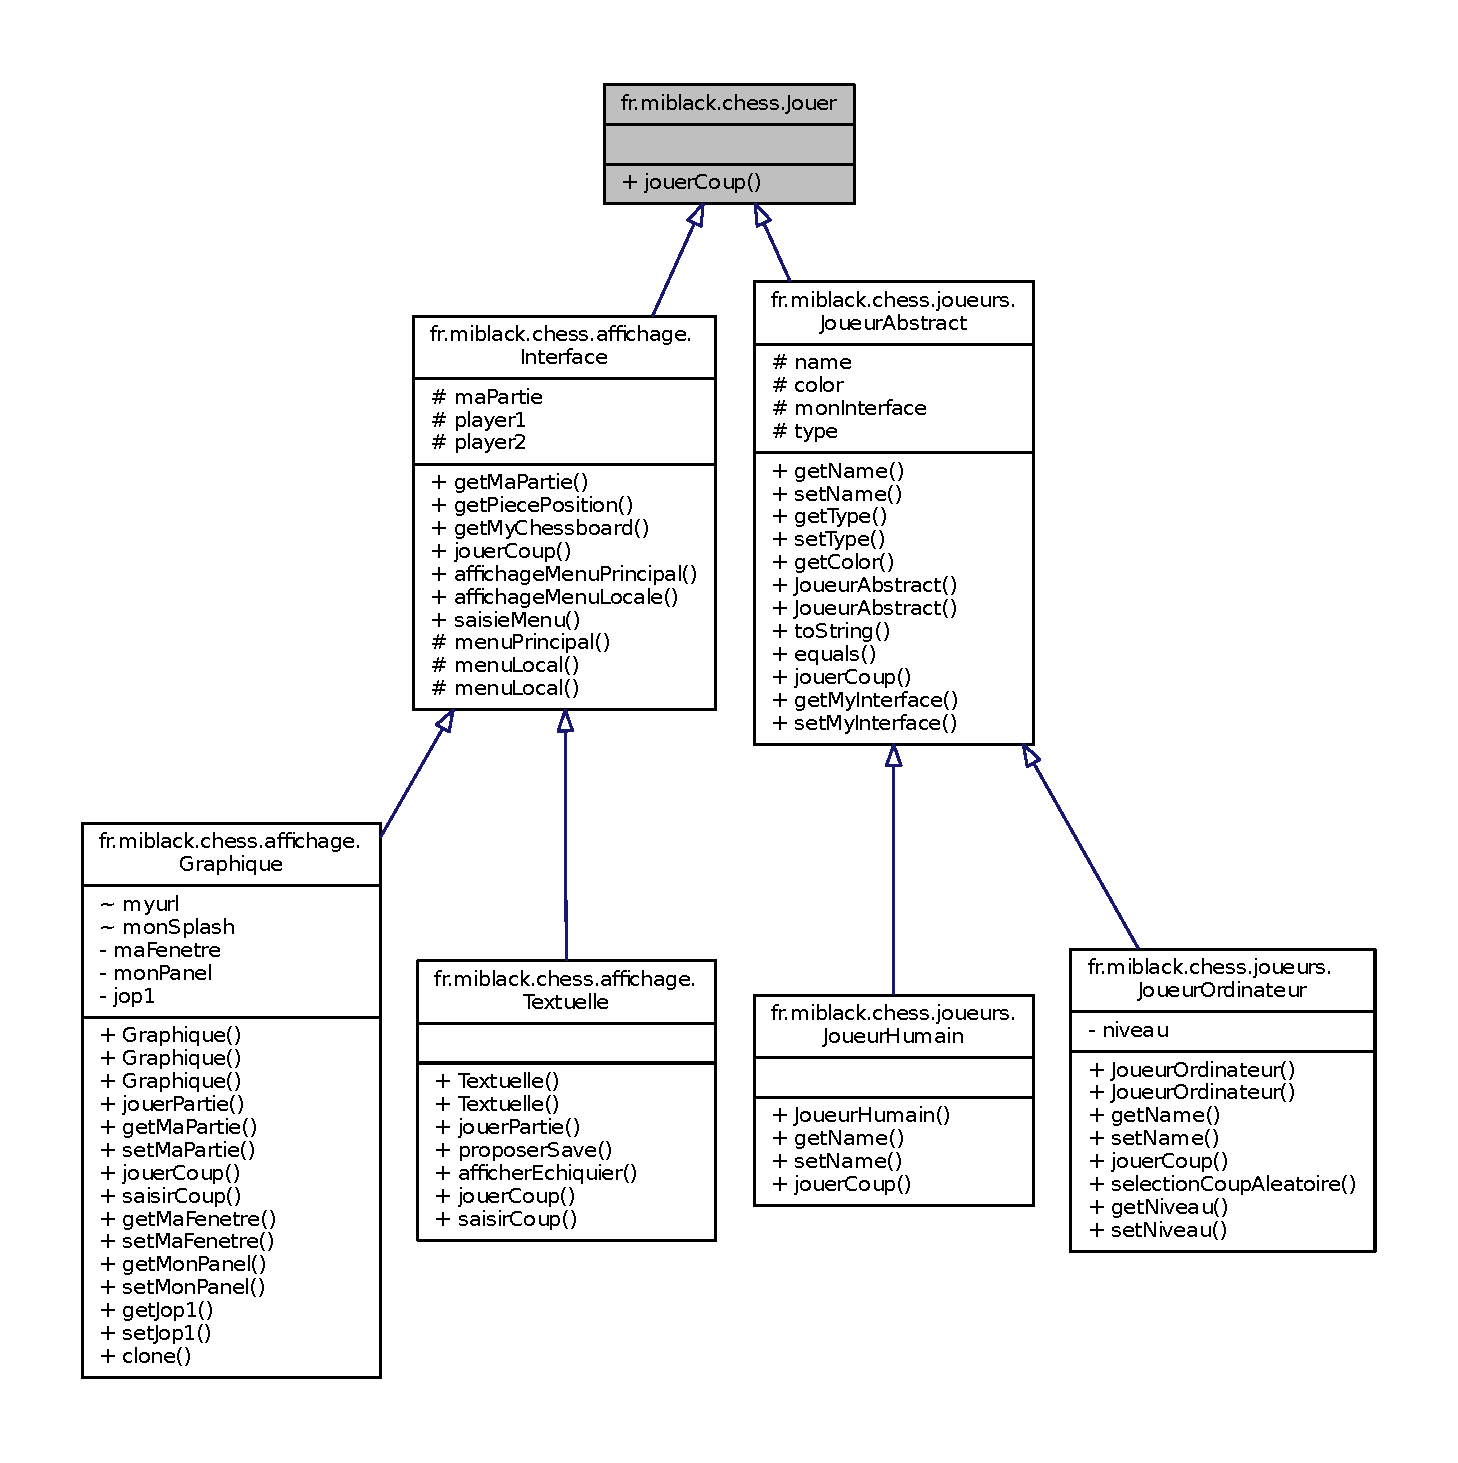
\includegraphics[width=350pt]{interfacefr_1_1miblack_1_1chess_1_1Jouer__inherit__graph}
\end{center}
\end{figure}


Collaboration diagram for fr.\-miblack.\-chess.\-Jouer\-:
\nopagebreak
\begin{figure}[H]
\begin{center}
\leavevmode
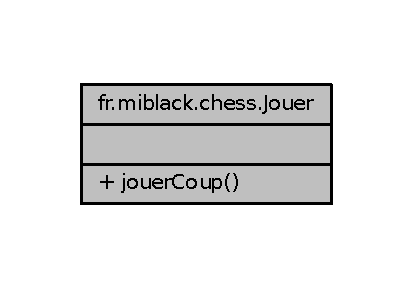
\includegraphics[width=198pt]{interfacefr_1_1miblack_1_1chess_1_1Jouer__coll__graph}
\end{center}
\end{figure}
\subsection*{Public Member Functions}
\begin{DoxyCompactItemize}
\item 
{\bf Coup} {\bf jouer\-Coup} ({\bf Partie} g)
\end{DoxyCompactItemize}


\subsection{Detailed Description}
Une interface qui défini comment on joue un coup \begin{DoxyAuthor}{Author}
mi-\/black 
\end{DoxyAuthor}


\subsection{Member Function Documentation}
\index{fr\-::miblack\-::chess\-::\-Jouer@{fr\-::miblack\-::chess\-::\-Jouer}!jouer\-Coup@{jouer\-Coup}}
\index{jouer\-Coup@{jouer\-Coup}!fr::miblack::chess::Jouer@{fr\-::miblack\-::chess\-::\-Jouer}}
\subsubsection[{jouer\-Coup}]{\setlength{\rightskip}{0pt plus 5cm}{\bf Coup} fr.\-miblack.\-chess.\-Jouer.\-jouer\-Coup (
\begin{DoxyParamCaption}
\item[{{\bf Partie}}]{g}
\end{DoxyParamCaption}
)}\label{interfacefr_1_1miblack_1_1chess_1_1Jouer_a37f671e9b8707e21e02ea5dfbe83937f}

\begin{DoxyParams}{Parameters}
{\em g} & une partie \\
\hline
\end{DoxyParams}
\begin{DoxyReturn}{Returns}
le coup Joué 
\end{DoxyReturn}


Implemented in {\bf fr.\-miblack.\-chess.\-affichage.\-Graphique} \doxyref{}{p.}{classfr_1_1miblack_1_1chess_1_1affichage_1_1Graphique_aa614e0e0e7cce0dac59276b59b04a549}, {\bf fr.\-miblack.\-chess.\-affichage.\-Textuelle} \doxyref{}{p.}{classfr_1_1miblack_1_1chess_1_1affichage_1_1Textuelle_a2fe98d89987be73eed0e7d666d16f3f5}, {\bf fr.\-miblack.\-chess.\-joueurs.\-Joueur\-Abstract} \doxyref{}{p.}{classfr_1_1miblack_1_1chess_1_1joueurs_1_1JoueurAbstract_a283cee619b9c52dbb333720b452838bf}, {\bf fr.\-miblack.\-chess.\-affichage.\-Interface} \doxyref{}{p.}{classfr_1_1miblack_1_1chess_1_1affichage_1_1Interface_a16a7abd6c521cb1e9cdafb5f586db68b}, {\bf fr.\-miblack.\-chess.\-joueurs.\-Joueur\-Ordinateur} \doxyref{}{p.}{classfr_1_1miblack_1_1chess_1_1joueurs_1_1JoueurOrdinateur_a382e1ffdba917346defae9ce101d6d57}, and {\bf fr.\-miblack.\-chess.\-joueurs.\-Joueur\-Humain} \doxyref{}{p.}{classfr_1_1miblack_1_1chess_1_1joueurs_1_1JoueurHumain_ab5068ae85407f93e5998f6844a65f483}.



The documentation for this interface was generated from the following file\-:\begin{DoxyCompactItemize}
\item 
fr/miblack/chess/{\bf Jouer.\-java}\end{DoxyCompactItemize}

\section{fr.\-miblack.\-chess.\-joueurs.\-Joueur\-Abstract Class Reference}
\label{classfr_1_1miblack_1_1chess_1_1joueurs_1_1JoueurAbstract}\index{fr.\-miblack.\-chess.\-joueurs.\-Joueur\-Abstract@{fr.\-miblack.\-chess.\-joueurs.\-Joueur\-Abstract}}
Inheritance diagram for fr.\-miblack.\-chess.\-joueurs.\-Joueur\-Abstract\-:\begin{figure}[H]
\begin{center}
\leavevmode
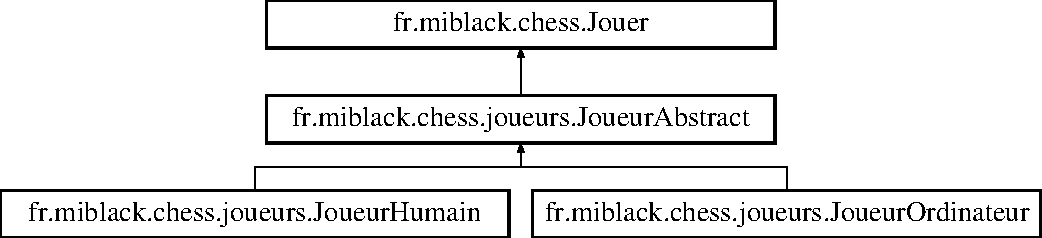
\includegraphics[height=3.000000cm]{classfr_1_1miblack_1_1chess_1_1joueurs_1_1JoueurAbstract}
\end{center}
\end{figure}
\subsection*{Public Member Functions}
\begin{DoxyCompactItemize}
\item 
String {\bf get\-Name} ()
\item 
void {\bf set\-Name} (String {\bf name})
\item 
String {\bf get\-Type} ()
\item 
void {\bf set\-Type} (String {\bf type})
\item 
{\bf Couleur} {\bf get\-Color} ()
\item 
{\bf Joueur\-Abstract} (String p1, {\bf Couleur} a, {\bf Interface} {\bf mon\-Interface})
\item 
{\bf Joueur\-Abstract} (String p1, {\bf Couleur} a)
\item 
String {\bf to\-String} ()
\item 
boolean {\bf equals} ({\bf Joueur\-Abstract} joueur)
\item 
abstract {\bf Coup} {\bf jouer\-Coup} ({\bf Partie} g)
\item 
{\bf Interface} {\bf get\-My\-Interface} ()
\item 
void {\bf set\-My\-Interface} ({\bf Interface} my\-Interface)
\end{DoxyCompactItemize}
\subsection*{Protected Attributes}
\begin{DoxyCompactItemize}
\item 
String {\bf name}
\item 
{\bf Couleur} {\bf color}
\item 
{\bf Interface} {\bf mon\-Interface}
\item 
String {\bf type}
\end{DoxyCompactItemize}


\subsection{Detailed Description}
\begin{DoxyAuthor}{Author}
mi-\/black 
\end{DoxyAuthor}


\subsection{Constructor \& Destructor Documentation}
\index{fr\-::miblack\-::chess\-::joueurs\-::\-Joueur\-Abstract@{fr\-::miblack\-::chess\-::joueurs\-::\-Joueur\-Abstract}!Joueur\-Abstract@{Joueur\-Abstract}}
\index{Joueur\-Abstract@{Joueur\-Abstract}!fr::miblack::chess::joueurs::JoueurAbstract@{fr\-::miblack\-::chess\-::joueurs\-::\-Joueur\-Abstract}}
\subsubsection[{Joueur\-Abstract}]{\setlength{\rightskip}{0pt plus 5cm}fr.\-miblack.\-chess.\-joueurs.\-Joueur\-Abstract.\-Joueur\-Abstract (
\begin{DoxyParamCaption}
\item[{String}]{p1, }
\item[{{\bf Couleur}}]{a, }
\item[{{\bf Interface}}]{mon\-Interface}
\end{DoxyParamCaption}
)}\label{classfr_1_1miblack_1_1chess_1_1joueurs_1_1JoueurAbstract_a9febf85fee46f81c6fd670439e6970d3}

\begin{DoxyParams}{Parameters}
{\em p1} & \\
\hline
{\em a} & couleur \\
\hline
{\em mon\-Interface} & \\
\hline
\end{DoxyParams}
\index{fr\-::miblack\-::chess\-::joueurs\-::\-Joueur\-Abstract@{fr\-::miblack\-::chess\-::joueurs\-::\-Joueur\-Abstract}!Joueur\-Abstract@{Joueur\-Abstract}}
\index{Joueur\-Abstract@{Joueur\-Abstract}!fr::miblack::chess::joueurs::JoueurAbstract@{fr\-::miblack\-::chess\-::joueurs\-::\-Joueur\-Abstract}}
\subsubsection[{Joueur\-Abstract}]{\setlength{\rightskip}{0pt plus 5cm}fr.\-miblack.\-chess.\-joueurs.\-Joueur\-Abstract.\-Joueur\-Abstract (
\begin{DoxyParamCaption}
\item[{String}]{p1, }
\item[{{\bf Couleur}}]{a}
\end{DoxyParamCaption}
)}\label{classfr_1_1miblack_1_1chess_1_1joueurs_1_1JoueurAbstract_a2e12b7b19220ec7f1339cdd08205c185}

\begin{DoxyParams}{Parameters}
{\em p1} & \\
\hline
{\em a} & couleur \\
\hline
\end{DoxyParams}


\subsection{Member Function Documentation}
\index{fr\-::miblack\-::chess\-::joueurs\-::\-Joueur\-Abstract@{fr\-::miblack\-::chess\-::joueurs\-::\-Joueur\-Abstract}!equals@{equals}}
\index{equals@{equals}!fr::miblack::chess::joueurs::JoueurAbstract@{fr\-::miblack\-::chess\-::joueurs\-::\-Joueur\-Abstract}}
\subsubsection[{equals}]{\setlength{\rightskip}{0pt plus 5cm}boolean fr.\-miblack.\-chess.\-joueurs.\-Joueur\-Abstract.\-equals (
\begin{DoxyParamCaption}
\item[{{\bf Joueur\-Abstract}}]{joueur}
\end{DoxyParamCaption}
)}\label{classfr_1_1miblack_1_1chess_1_1joueurs_1_1JoueurAbstract_a1efdbeb135b7007e6cdc7ac62fa717b9}
\begin{DoxyReturn}{Returns}

\end{DoxyReturn}
\index{fr\-::miblack\-::chess\-::joueurs\-::\-Joueur\-Abstract@{fr\-::miblack\-::chess\-::joueurs\-::\-Joueur\-Abstract}!get\-Color@{get\-Color}}
\index{get\-Color@{get\-Color}!fr::miblack::chess::joueurs::JoueurAbstract@{fr\-::miblack\-::chess\-::joueurs\-::\-Joueur\-Abstract}}
\subsubsection[{get\-Color}]{\setlength{\rightskip}{0pt plus 5cm}{\bf Couleur} fr.\-miblack.\-chess.\-joueurs.\-Joueur\-Abstract.\-get\-Color (
\begin{DoxyParamCaption}
{}
\end{DoxyParamCaption}
)}\label{classfr_1_1miblack_1_1chess_1_1joueurs_1_1JoueurAbstract_ab7b13d1563d346a00fbbc69cf3186d62}
\begin{DoxyReturn}{Returns}

\end{DoxyReturn}
\index{fr\-::miblack\-::chess\-::joueurs\-::\-Joueur\-Abstract@{fr\-::miblack\-::chess\-::joueurs\-::\-Joueur\-Abstract}!get\-My\-Interface@{get\-My\-Interface}}
\index{get\-My\-Interface@{get\-My\-Interface}!fr::miblack::chess::joueurs::JoueurAbstract@{fr\-::miblack\-::chess\-::joueurs\-::\-Joueur\-Abstract}}
\subsubsection[{get\-My\-Interface}]{\setlength{\rightskip}{0pt plus 5cm}{\bf Interface} fr.\-miblack.\-chess.\-joueurs.\-Joueur\-Abstract.\-get\-My\-Interface (
\begin{DoxyParamCaption}
{}
\end{DoxyParamCaption}
)}\label{classfr_1_1miblack_1_1chess_1_1joueurs_1_1JoueurAbstract_a2dc46821c92edc43494766d99bceebcd}
\begin{DoxyReturn}{Returns}

\end{DoxyReturn}
\index{fr\-::miblack\-::chess\-::joueurs\-::\-Joueur\-Abstract@{fr\-::miblack\-::chess\-::joueurs\-::\-Joueur\-Abstract}!get\-Name@{get\-Name}}
\index{get\-Name@{get\-Name}!fr::miblack::chess::joueurs::JoueurAbstract@{fr\-::miblack\-::chess\-::joueurs\-::\-Joueur\-Abstract}}
\subsubsection[{get\-Name}]{\setlength{\rightskip}{0pt plus 5cm}String fr.\-miblack.\-chess.\-joueurs.\-Joueur\-Abstract.\-get\-Name (
\begin{DoxyParamCaption}
{}
\end{DoxyParamCaption}
)}\label{classfr_1_1miblack_1_1chess_1_1joueurs_1_1JoueurAbstract_ad29f62a9a391371f63122a120a472f38}
\begin{DoxyReturn}{Returns}

\end{DoxyReturn}


Reimplemented in {\bf fr.\-miblack.\-chess.\-joueurs.\-Joueur\-Ordinateur} \doxyref{}{p.}{classfr_1_1miblack_1_1chess_1_1joueurs_1_1JoueurOrdinateur_afff6843c3b7fb2653130425ed0d9b8ff}, and {\bf fr.\-miblack.\-chess.\-joueurs.\-Joueur\-Humain} \doxyref{}{p.}{classfr_1_1miblack_1_1chess_1_1joueurs_1_1JoueurHumain_a78e0874aab2e1aa8f75e311bda43d578}.

\index{fr\-::miblack\-::chess\-::joueurs\-::\-Joueur\-Abstract@{fr\-::miblack\-::chess\-::joueurs\-::\-Joueur\-Abstract}!get\-Type@{get\-Type}}
\index{get\-Type@{get\-Type}!fr::miblack::chess::joueurs::JoueurAbstract@{fr\-::miblack\-::chess\-::joueurs\-::\-Joueur\-Abstract}}
\subsubsection[{get\-Type}]{\setlength{\rightskip}{0pt plus 5cm}String fr.\-miblack.\-chess.\-joueurs.\-Joueur\-Abstract.\-get\-Type (
\begin{DoxyParamCaption}
{}
\end{DoxyParamCaption}
)}\label{classfr_1_1miblack_1_1chess_1_1joueurs_1_1JoueurAbstract_a2ab945f71218a830d7cb6d30805bb8a4}
\begin{DoxyReturn}{Returns}

\end{DoxyReturn}
\index{fr\-::miblack\-::chess\-::joueurs\-::\-Joueur\-Abstract@{fr\-::miblack\-::chess\-::joueurs\-::\-Joueur\-Abstract}!jouer\-Coup@{jouer\-Coup}}
\index{jouer\-Coup@{jouer\-Coup}!fr::miblack::chess::joueurs::JoueurAbstract@{fr\-::miblack\-::chess\-::joueurs\-::\-Joueur\-Abstract}}
\subsubsection[{jouer\-Coup}]{\setlength{\rightskip}{0pt plus 5cm}abstract {\bf Coup} fr.\-miblack.\-chess.\-joueurs.\-Joueur\-Abstract.\-jouer\-Coup (
\begin{DoxyParamCaption}
\item[{{\bf Partie}}]{g}
\end{DoxyParamCaption}
)\hspace{0.3cm}{\ttfamily [pure virtual]}}\label{classfr_1_1miblack_1_1chess_1_1joueurs_1_1JoueurAbstract_a283cee619b9c52dbb333720b452838bf}

\begin{DoxyParams}{Parameters}
{\em g} & une partie \\
\hline
\end{DoxyParams}
\begin{DoxyReturn}{Returns}
le coup Joué 
\end{DoxyReturn}


Implements {\bf fr.\-miblack.\-chess.\-Jouer} \doxyref{}{p.}{interfacefr_1_1miblack_1_1chess_1_1Jouer_a37f671e9b8707e21e02ea5dfbe83937f}.



Implemented in {\bf fr.\-miblack.\-chess.\-joueurs.\-Joueur\-Ordinateur} \doxyref{}{p.}{classfr_1_1miblack_1_1chess_1_1joueurs_1_1JoueurOrdinateur_a382e1ffdba917346defae9ce101d6d57}, and {\bf fr.\-miblack.\-chess.\-joueurs.\-Joueur\-Humain} \doxyref{}{p.}{classfr_1_1miblack_1_1chess_1_1joueurs_1_1JoueurHumain_ab5068ae85407f93e5998f6844a65f483}.

\index{fr\-::miblack\-::chess\-::joueurs\-::\-Joueur\-Abstract@{fr\-::miblack\-::chess\-::joueurs\-::\-Joueur\-Abstract}!set\-My\-Interface@{set\-My\-Interface}}
\index{set\-My\-Interface@{set\-My\-Interface}!fr::miblack::chess::joueurs::JoueurAbstract@{fr\-::miblack\-::chess\-::joueurs\-::\-Joueur\-Abstract}}
\subsubsection[{set\-My\-Interface}]{\setlength{\rightskip}{0pt plus 5cm}void fr.\-miblack.\-chess.\-joueurs.\-Joueur\-Abstract.\-set\-My\-Interface (
\begin{DoxyParamCaption}
\item[{{\bf Interface}}]{my\-Interface}
\end{DoxyParamCaption}
)}\label{classfr_1_1miblack_1_1chess_1_1joueurs_1_1JoueurAbstract_aedc32fc291dff3d38d91f343b2d87c72}
\begin{DoxyReturn}{Returns}

\end{DoxyReturn}
\index{fr\-::miblack\-::chess\-::joueurs\-::\-Joueur\-Abstract@{fr\-::miblack\-::chess\-::joueurs\-::\-Joueur\-Abstract}!set\-Name@{set\-Name}}
\index{set\-Name@{set\-Name}!fr::miblack::chess::joueurs::JoueurAbstract@{fr\-::miblack\-::chess\-::joueurs\-::\-Joueur\-Abstract}}
\subsubsection[{set\-Name}]{\setlength{\rightskip}{0pt plus 5cm}void fr.\-miblack.\-chess.\-joueurs.\-Joueur\-Abstract.\-set\-Name (
\begin{DoxyParamCaption}
\item[{String}]{name}
\end{DoxyParamCaption}
)}\label{classfr_1_1miblack_1_1chess_1_1joueurs_1_1JoueurAbstract_af24355af3066519a244add148335a51f}

\begin{DoxyParams}{Parameters}
{\em name} & \\
\hline
\end{DoxyParams}


Reimplemented in {\bf fr.\-miblack.\-chess.\-joueurs.\-Joueur\-Ordinateur} \doxyref{}{p.}{classfr_1_1miblack_1_1chess_1_1joueurs_1_1JoueurOrdinateur_a3238d4bba49de2c2dd22e777c80c2228}, and {\bf fr.\-miblack.\-chess.\-joueurs.\-Joueur\-Humain} \doxyref{}{p.}{classfr_1_1miblack_1_1chess_1_1joueurs_1_1JoueurHumain_a60a4f6db173cd980d25feee430d5f32e}.

\index{fr\-::miblack\-::chess\-::joueurs\-::\-Joueur\-Abstract@{fr\-::miblack\-::chess\-::joueurs\-::\-Joueur\-Abstract}!set\-Type@{set\-Type}}
\index{set\-Type@{set\-Type}!fr::miblack::chess::joueurs::JoueurAbstract@{fr\-::miblack\-::chess\-::joueurs\-::\-Joueur\-Abstract}}
\subsubsection[{set\-Type}]{\setlength{\rightskip}{0pt plus 5cm}void fr.\-miblack.\-chess.\-joueurs.\-Joueur\-Abstract.\-set\-Type (
\begin{DoxyParamCaption}
\item[{String}]{type}
\end{DoxyParamCaption}
)}\label{classfr_1_1miblack_1_1chess_1_1joueurs_1_1JoueurAbstract_ac33805c0cd6b54a54747f9b060d149e9}

\begin{DoxyParams}{Parameters}
{\em type} & \\
\hline
\end{DoxyParams}
\index{fr\-::miblack\-::chess\-::joueurs\-::\-Joueur\-Abstract@{fr\-::miblack\-::chess\-::joueurs\-::\-Joueur\-Abstract}!to\-String@{to\-String}}
\index{to\-String@{to\-String}!fr::miblack::chess::joueurs::JoueurAbstract@{fr\-::miblack\-::chess\-::joueurs\-::\-Joueur\-Abstract}}
\subsubsection[{to\-String}]{\setlength{\rightskip}{0pt plus 5cm}String fr.\-miblack.\-chess.\-joueurs.\-Joueur\-Abstract.\-to\-String (
\begin{DoxyParamCaption}
{}
\end{DoxyParamCaption}
)}\label{classfr_1_1miblack_1_1chess_1_1joueurs_1_1JoueurAbstract_af0b06b7381660970ed0718b4ccefc7a8}
\begin{DoxyReturn}{Returns}

\end{DoxyReturn}


\subsection{Member Data Documentation}
\index{fr\-::miblack\-::chess\-::joueurs\-::\-Joueur\-Abstract@{fr\-::miblack\-::chess\-::joueurs\-::\-Joueur\-Abstract}!color@{color}}
\index{color@{color}!fr::miblack::chess::joueurs::JoueurAbstract@{fr\-::miblack\-::chess\-::joueurs\-::\-Joueur\-Abstract}}
\subsubsection[{color}]{\setlength{\rightskip}{0pt plus 5cm}{\bf Couleur} fr.\-miblack.\-chess.\-joueurs.\-Joueur\-Abstract.\-color\hspace{0.3cm}{\ttfamily [protected]}}\label{classfr_1_1miblack_1_1chess_1_1joueurs_1_1JoueurAbstract_a3f2c489a75d40645a0a388ab54e5430b}
la couleur \index{fr\-::miblack\-::chess\-::joueurs\-::\-Joueur\-Abstract@{fr\-::miblack\-::chess\-::joueurs\-::\-Joueur\-Abstract}!mon\-Interface@{mon\-Interface}}
\index{mon\-Interface@{mon\-Interface}!fr::miblack::chess::joueurs::JoueurAbstract@{fr\-::miblack\-::chess\-::joueurs\-::\-Joueur\-Abstract}}
\subsubsection[{mon\-Interface}]{\setlength{\rightskip}{0pt plus 5cm}{\bf Interface} fr.\-miblack.\-chess.\-joueurs.\-Joueur\-Abstract.\-mon\-Interface\hspace{0.3cm}{\ttfamily [protected]}}\label{classfr_1_1miblack_1_1chess_1_1joueurs_1_1JoueurAbstract_a9a240d43c6f2fd69dc7ee64dad94d129}
l'interface utilisé \index{fr\-::miblack\-::chess\-::joueurs\-::\-Joueur\-Abstract@{fr\-::miblack\-::chess\-::joueurs\-::\-Joueur\-Abstract}!name@{name}}
\index{name@{name}!fr::miblack::chess::joueurs::JoueurAbstract@{fr\-::miblack\-::chess\-::joueurs\-::\-Joueur\-Abstract}}
\subsubsection[{name}]{\setlength{\rightskip}{0pt plus 5cm}String fr.\-miblack.\-chess.\-joueurs.\-Joueur\-Abstract.\-name\hspace{0.3cm}{\ttfamily [protected]}}\label{classfr_1_1miblack_1_1chess_1_1joueurs_1_1JoueurAbstract_a59d284fd4eb4f03e28a1f28950be8acd}
le nom \index{fr\-::miblack\-::chess\-::joueurs\-::\-Joueur\-Abstract@{fr\-::miblack\-::chess\-::joueurs\-::\-Joueur\-Abstract}!type@{type}}
\index{type@{type}!fr::miblack::chess::joueurs::JoueurAbstract@{fr\-::miblack\-::chess\-::joueurs\-::\-Joueur\-Abstract}}
\subsubsection[{type}]{\setlength{\rightskip}{0pt plus 5cm}String fr.\-miblack.\-chess.\-joueurs.\-Joueur\-Abstract.\-type\hspace{0.3cm}{\ttfamily [protected]}}\label{classfr_1_1miblack_1_1chess_1_1joueurs_1_1JoueurAbstract_a9d8b6e453a41778f9629e98088495fcf}
le type 

The documentation for this class was generated from the following file\-:\begin{DoxyCompactItemize}
\item 
fr/miblack/chess/joueurs/Joueur\-Abstract.\-java\end{DoxyCompactItemize}

\section{fr.\-miblack.\-chess.\-joueurs.\-Joueur\-Humain Class Reference}
\label{classfr_1_1miblack_1_1chess_1_1joueurs_1_1JoueurHumain}\index{fr.\-miblack.\-chess.\-joueurs.\-Joueur\-Humain@{fr.\-miblack.\-chess.\-joueurs.\-Joueur\-Humain}}


Inheritance diagram for fr.\-miblack.\-chess.\-joueurs.\-Joueur\-Humain\-:
\nopagebreak
\begin{figure}[H]
\begin{center}
\leavevmode
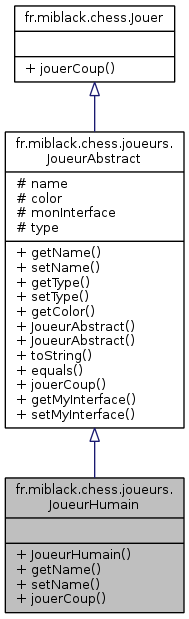
\includegraphics[width=214pt]{classfr_1_1miblack_1_1chess_1_1joueurs_1_1JoueurHumain__inherit__graph}
\end{center}
\end{figure}


Collaboration diagram for fr.\-miblack.\-chess.\-joueurs.\-Joueur\-Humain\-:
\nopagebreak
\begin{figure}[H]
\begin{center}
\leavevmode
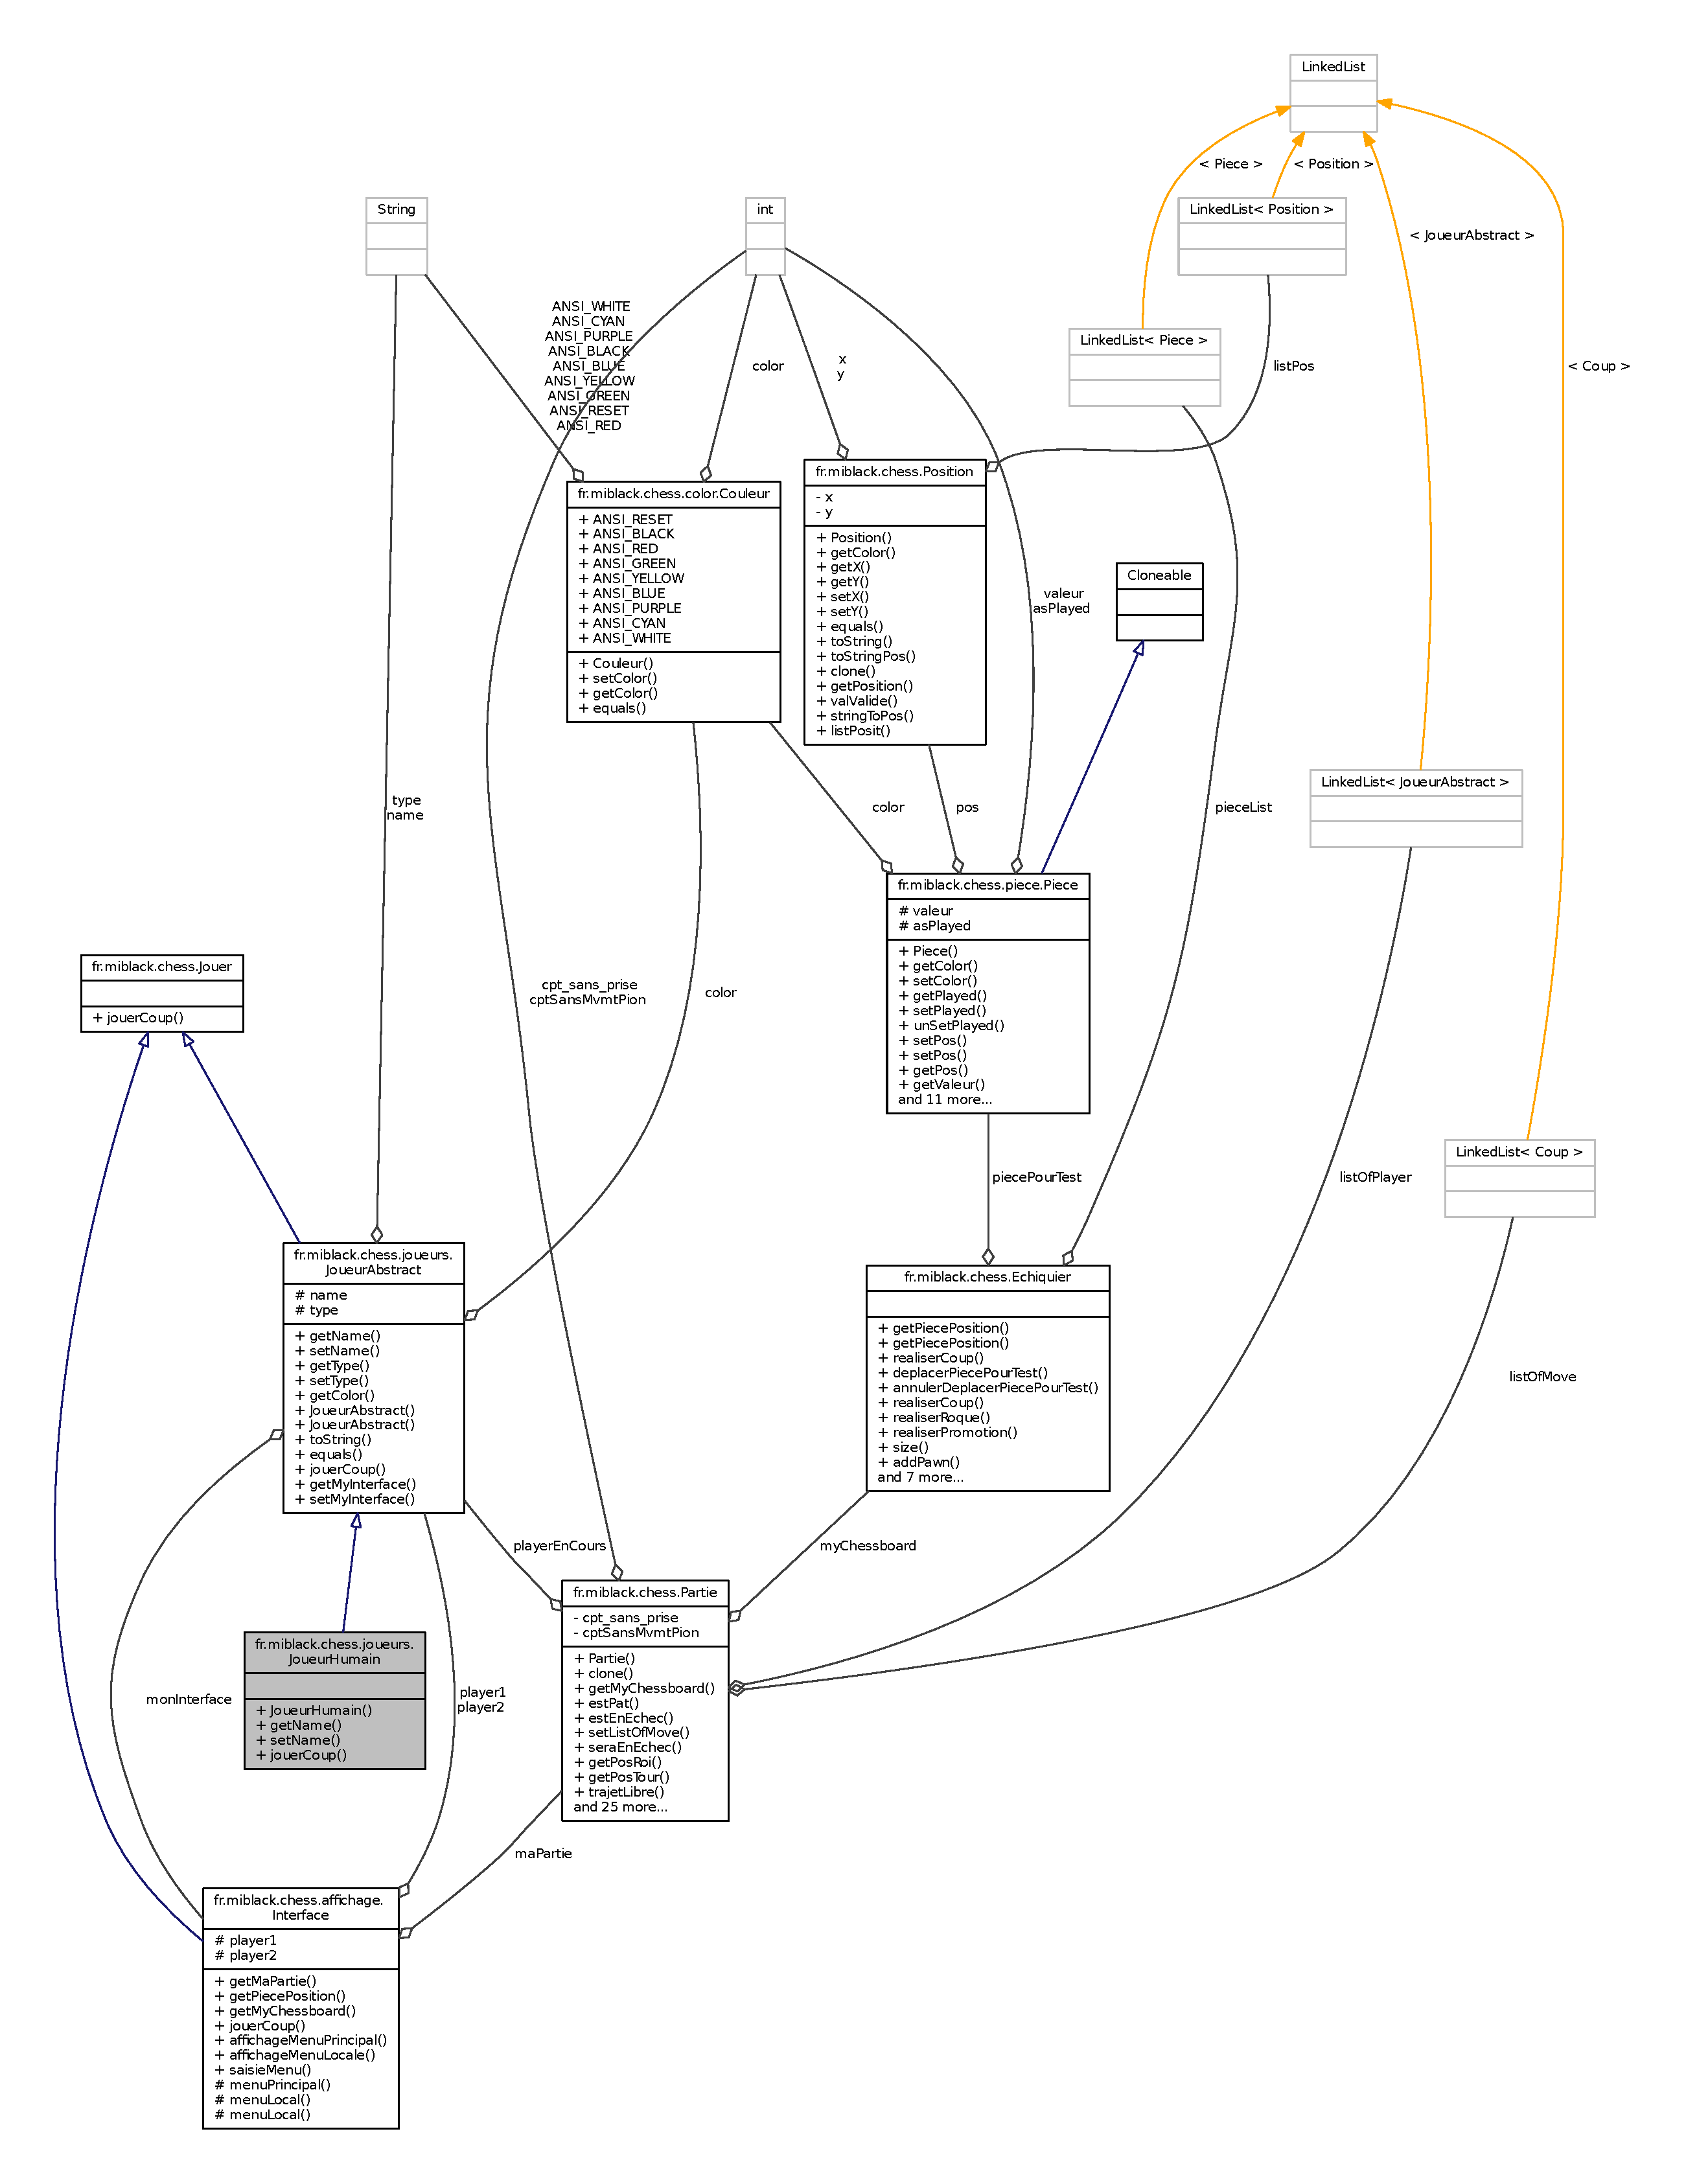
\includegraphics[width=350pt]{classfr_1_1miblack_1_1chess_1_1joueurs_1_1JoueurHumain__coll__graph}
\end{center}
\end{figure}
\subsection*{Public Member Functions}
\begin{DoxyCompactItemize}
\item 
{\bf Joueur\-Humain} (String p1, {\bf Couleur} a, {\bf Interface} {\bf mon\-Interface})
\item 
String {\bf get\-Name} ()
\item 
void {\bf set\-Name} (String {\bf name})
\item 
{\bf Coup} {\bf jouer\-Coup} ({\bf Partie} a)
\end{DoxyCompactItemize}
\subsection*{Additional Inherited Members}


\subsection{Detailed Description}
\begin{DoxyAuthor}{Author}
mi-\/black 
\end{DoxyAuthor}


\subsection{Constructor \& Destructor Documentation}
\index{fr\-::miblack\-::chess\-::joueurs\-::\-Joueur\-Humain@{fr\-::miblack\-::chess\-::joueurs\-::\-Joueur\-Humain}!Joueur\-Humain@{Joueur\-Humain}}
\index{Joueur\-Humain@{Joueur\-Humain}!fr::miblack::chess::joueurs::JoueurHumain@{fr\-::miblack\-::chess\-::joueurs\-::\-Joueur\-Humain}}
\subsubsection[{Joueur\-Humain}]{\setlength{\rightskip}{0pt plus 5cm}fr.\-miblack.\-chess.\-joueurs.\-Joueur\-Humain.\-Joueur\-Humain (
\begin{DoxyParamCaption}
\item[{String}]{p1, }
\item[{{\bf Couleur}}]{a, }
\item[{{\bf Interface}}]{mon\-Interface}
\end{DoxyParamCaption}
)}\label{classfr_1_1miblack_1_1chess_1_1joueurs_1_1JoueurHumain_a9b8acadd84c9a3fa1ab48601397c1633}

\begin{DoxyParams}{Parameters}
{\em p1} & \\
\hline
{\em a} & la couleur \\
\hline
{\em mon\-Interface} & \\
\hline
\end{DoxyParams}


\subsection{Member Function Documentation}
\index{fr\-::miblack\-::chess\-::joueurs\-::\-Joueur\-Humain@{fr\-::miblack\-::chess\-::joueurs\-::\-Joueur\-Humain}!get\-Name@{get\-Name}}
\index{get\-Name@{get\-Name}!fr::miblack::chess::joueurs::JoueurHumain@{fr\-::miblack\-::chess\-::joueurs\-::\-Joueur\-Humain}}
\subsubsection[{get\-Name}]{\setlength{\rightskip}{0pt plus 5cm}String fr.\-miblack.\-chess.\-joueurs.\-Joueur\-Humain.\-get\-Name (
\begin{DoxyParamCaption}
{}
\end{DoxyParamCaption}
)}\label{classfr_1_1miblack_1_1chess_1_1joueurs_1_1JoueurHumain_a78e0874aab2e1aa8f75e311bda43d578}
\begin{DoxyReturn}{Returns}

\end{DoxyReturn}


Reimplemented from {\bf fr.\-miblack.\-chess.\-joueurs.\-Joueur\-Abstract} \doxyref{}{p.}{classfr_1_1miblack_1_1chess_1_1joueurs_1_1JoueurAbstract_ad29f62a9a391371f63122a120a472f38}.

\index{fr\-::miblack\-::chess\-::joueurs\-::\-Joueur\-Humain@{fr\-::miblack\-::chess\-::joueurs\-::\-Joueur\-Humain}!jouer\-Coup@{jouer\-Coup}}
\index{jouer\-Coup@{jouer\-Coup}!fr::miblack::chess::joueurs::JoueurHumain@{fr\-::miblack\-::chess\-::joueurs\-::\-Joueur\-Humain}}
\subsubsection[{jouer\-Coup}]{\setlength{\rightskip}{0pt plus 5cm}{\bf Coup} fr.\-miblack.\-chess.\-joueurs.\-Joueur\-Humain.\-jouer\-Coup (
\begin{DoxyParamCaption}
\item[{{\bf Partie}}]{g}
\end{DoxyParamCaption}
)\hspace{0.3cm}{\ttfamily [virtual]}}\label{classfr_1_1miblack_1_1chess_1_1joueurs_1_1JoueurHumain_ab5068ae85407f93e5998f6844a65f483}

\begin{DoxyParams}{Parameters}
{\em g} & une partie \\
\hline
\end{DoxyParams}
\begin{DoxyReturn}{Returns}
le coup Joué 
\end{DoxyReturn}


Implements {\bf fr.\-miblack.\-chess.\-joueurs.\-Joueur\-Abstract} \doxyref{}{p.}{classfr_1_1miblack_1_1chess_1_1joueurs_1_1JoueurAbstract_a283cee619b9c52dbb333720b452838bf}.

\index{fr\-::miblack\-::chess\-::joueurs\-::\-Joueur\-Humain@{fr\-::miblack\-::chess\-::joueurs\-::\-Joueur\-Humain}!set\-Name@{set\-Name}}
\index{set\-Name@{set\-Name}!fr::miblack::chess::joueurs::JoueurHumain@{fr\-::miblack\-::chess\-::joueurs\-::\-Joueur\-Humain}}
\subsubsection[{set\-Name}]{\setlength{\rightskip}{0pt plus 5cm}void fr.\-miblack.\-chess.\-joueurs.\-Joueur\-Humain.\-set\-Name (
\begin{DoxyParamCaption}
\item[{String}]{name}
\end{DoxyParamCaption}
)}\label{classfr_1_1miblack_1_1chess_1_1joueurs_1_1JoueurHumain_a60a4f6db173cd980d25feee430d5f32e}

\begin{DoxyParams}{Parameters}
{\em name} & \\
\hline
\end{DoxyParams}


Reimplemented from {\bf fr.\-miblack.\-chess.\-joueurs.\-Joueur\-Abstract} \doxyref{}{p.}{classfr_1_1miblack_1_1chess_1_1joueurs_1_1JoueurAbstract_af24355af3066519a244add148335a51f}.



The documentation for this class was generated from the following file\-:\begin{DoxyCompactItemize}
\item 
fr/miblack/chess/joueurs/{\bf Joueur\-Humain.\-java}\end{DoxyCompactItemize}

\section{fr.\-miblack.\-chess.\-joueurs.\-Joueur\-Ordinateur Class Reference}
\label{classfr_1_1miblack_1_1chess_1_1joueurs_1_1JoueurOrdinateur}\index{fr.\-miblack.\-chess.\-joueurs.\-Joueur\-Ordinateur@{fr.\-miblack.\-chess.\-joueurs.\-Joueur\-Ordinateur}}


Inheritance diagram for fr.\-miblack.\-chess.\-joueurs.\-Joueur\-Ordinateur\-:
\nopagebreak
\begin{figure}[H]
\begin{center}
\leavevmode
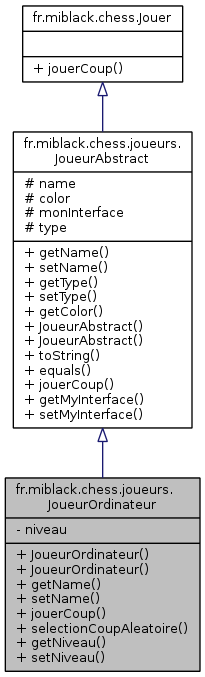
\includegraphics[height=550pt]{classfr_1_1miblack_1_1chess_1_1joueurs_1_1JoueurOrdinateur__inherit__graph}
\end{center}
\end{figure}


Collaboration diagram for fr.\-miblack.\-chess.\-joueurs.\-Joueur\-Ordinateur\-:
\nopagebreak
\begin{figure}[H]
\begin{center}
\leavevmode
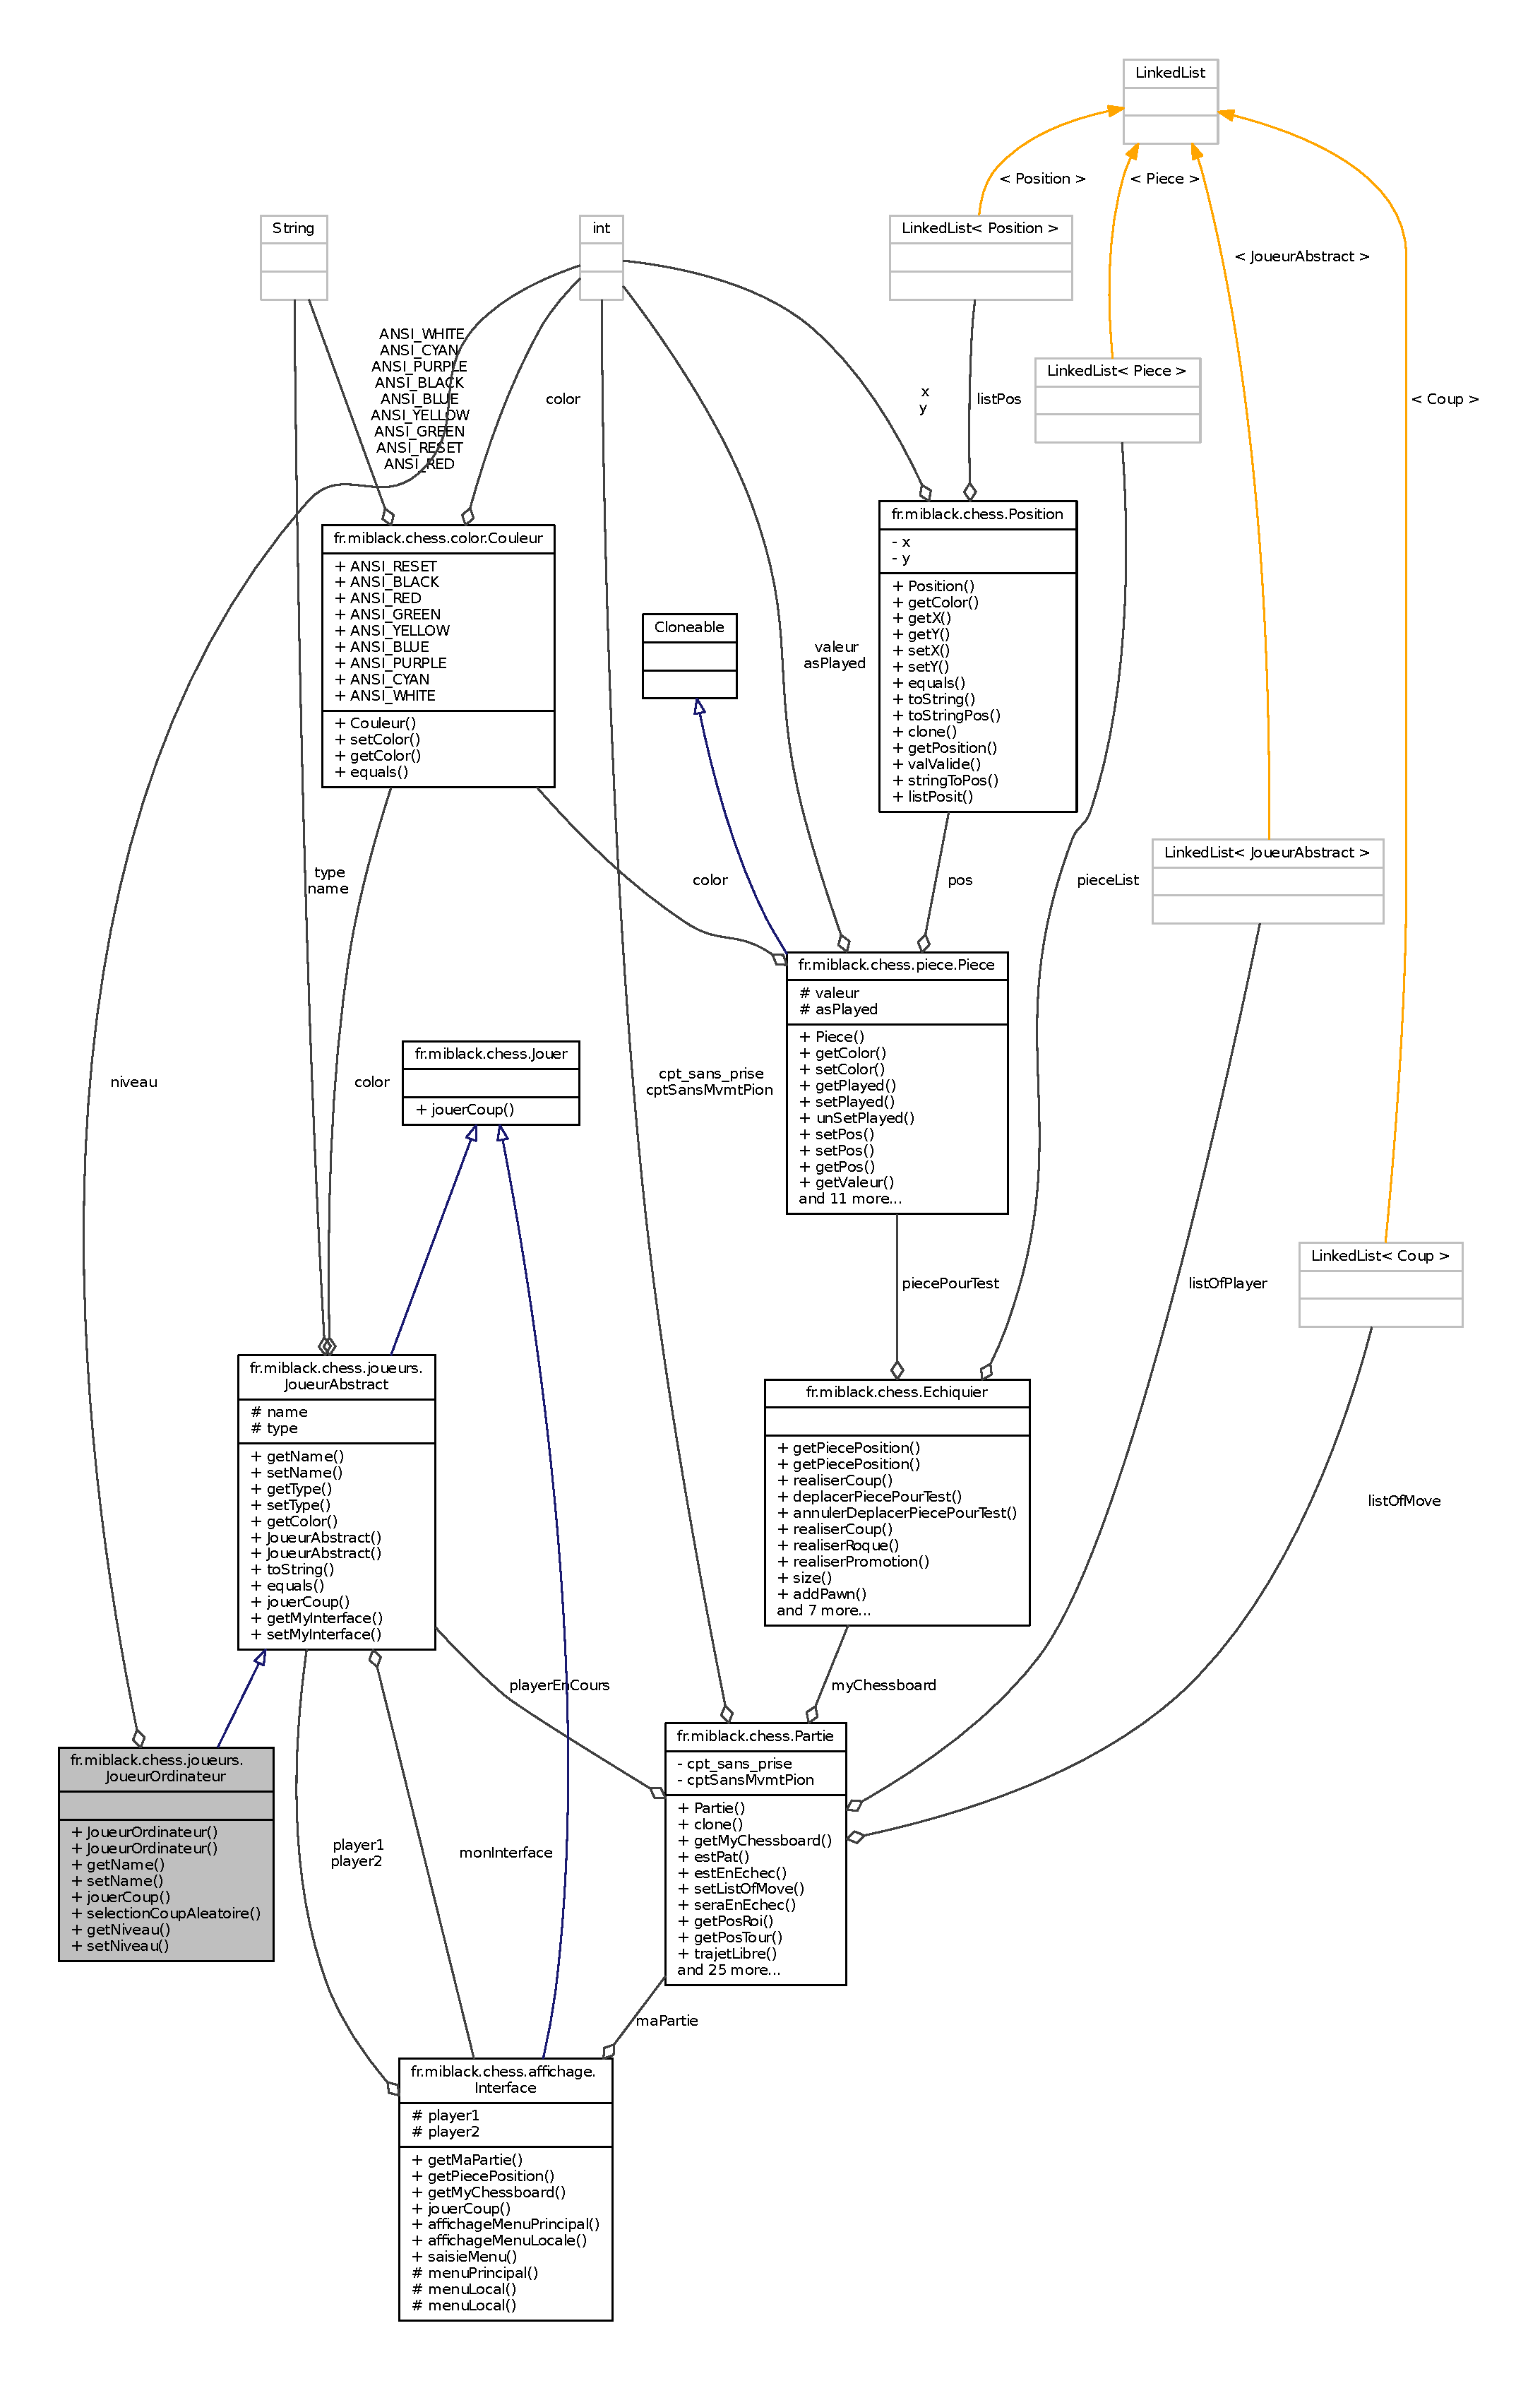
\includegraphics[width=350pt]{classfr_1_1miblack_1_1chess_1_1joueurs_1_1JoueurOrdinateur__coll__graph}
\end{center}
\end{figure}
\subsection*{Public Member Functions}
\begin{DoxyCompactItemize}
\item 
{\bf Joueur\-Ordinateur} (String p1, {\bf Couleur} a, {\bf Interface} {\bf mon\-Interface})
\item 
{\bf Joueur\-Ordinateur} (String p1, {\bf Couleur} a, {\bf Interface} {\bf mon\-Interface}, int {\bf niveau})
\item 
String {\bf get\-Name} ()
\item 
void {\bf set\-Name} (String {\bf name})
\item 
{\bf Coup} {\bf jouer\-Coup} ({\bf Partie} a)
\item 
{\bf Coup} {\bf selection\-Coup\-Aleatoire} ({\bf Partie} a)
\item 
int {\bf get\-Niveau} ()
\item 
void {\bf set\-Niveau} (int {\bf niveau})
\end{DoxyCompactItemize}
\subsection*{Private Attributes}
\begin{DoxyCompactItemize}
\item 
int {\bf niveau}
\end{DoxyCompactItemize}
\subsection*{Additional Inherited Members}


\subsection{Detailed Description}
\begin{DoxyAuthor}{Author}
mi-\/black 
\end{DoxyAuthor}


\subsection{Constructor \& Destructor Documentation}
\index{fr\-::miblack\-::chess\-::joueurs\-::\-Joueur\-Ordinateur@{fr\-::miblack\-::chess\-::joueurs\-::\-Joueur\-Ordinateur}!Joueur\-Ordinateur@{Joueur\-Ordinateur}}
\index{Joueur\-Ordinateur@{Joueur\-Ordinateur}!fr::miblack::chess::joueurs::JoueurOrdinateur@{fr\-::miblack\-::chess\-::joueurs\-::\-Joueur\-Ordinateur}}
\subsubsection[{Joueur\-Ordinateur}]{\setlength{\rightskip}{0pt plus 5cm}fr.\-miblack.\-chess.\-joueurs.\-Joueur\-Ordinateur.\-Joueur\-Ordinateur (
\begin{DoxyParamCaption}
\item[{String}]{p1, }
\item[{{\bf Couleur}}]{a, }
\item[{{\bf Interface}}]{mon\-Interface}
\end{DoxyParamCaption}
)}\label{classfr_1_1miblack_1_1chess_1_1joueurs_1_1JoueurOrdinateur_aead5ad3182acd106b70f2edf99cea73f}

\begin{DoxyParams}{Parameters}
{\em p1} & \\
\hline
{\em a} & couleur \\
\hline
{\em mon\-Interface} & \\
\hline
\end{DoxyParams}
\index{fr\-::miblack\-::chess\-::joueurs\-::\-Joueur\-Ordinateur@{fr\-::miblack\-::chess\-::joueurs\-::\-Joueur\-Ordinateur}!Joueur\-Ordinateur@{Joueur\-Ordinateur}}
\index{Joueur\-Ordinateur@{Joueur\-Ordinateur}!fr::miblack::chess::joueurs::JoueurOrdinateur@{fr\-::miblack\-::chess\-::joueurs\-::\-Joueur\-Ordinateur}}
\subsubsection[{Joueur\-Ordinateur}]{\setlength{\rightskip}{0pt plus 5cm}fr.\-miblack.\-chess.\-joueurs.\-Joueur\-Ordinateur.\-Joueur\-Ordinateur (
\begin{DoxyParamCaption}
\item[{String}]{p1, }
\item[{{\bf Couleur}}]{a, }
\item[{{\bf Interface}}]{mon\-Interface, }
\item[{int}]{niveau}
\end{DoxyParamCaption}
)}\label{classfr_1_1miblack_1_1chess_1_1joueurs_1_1JoueurOrdinateur_ac3e9d45adf1b5970f8b3813ff9f7ab43}

\begin{DoxyParams}{Parameters}
{\em p1} & \\
\hline
{\em a} & \\
\hline
{\em mon\-Interface} & \\
\hline
{\em niveau} & \\
\hline
\end{DoxyParams}


\subsection{Member Function Documentation}
\index{fr\-::miblack\-::chess\-::joueurs\-::\-Joueur\-Ordinateur@{fr\-::miblack\-::chess\-::joueurs\-::\-Joueur\-Ordinateur}!get\-Name@{get\-Name}}
\index{get\-Name@{get\-Name}!fr::miblack::chess::joueurs::JoueurOrdinateur@{fr\-::miblack\-::chess\-::joueurs\-::\-Joueur\-Ordinateur}}
\subsubsection[{get\-Name}]{\setlength{\rightskip}{0pt plus 5cm}String fr.\-miblack.\-chess.\-joueurs.\-Joueur\-Ordinateur.\-get\-Name (
\begin{DoxyParamCaption}
{}
\end{DoxyParamCaption}
)}\label{classfr_1_1miblack_1_1chess_1_1joueurs_1_1JoueurOrdinateur_afff6843c3b7fb2653130425ed0d9b8ff}
\begin{DoxyReturn}{Returns}

\end{DoxyReturn}


Reimplemented from {\bf fr.\-miblack.\-chess.\-joueurs.\-Joueur\-Abstract} \doxyref{}{p.}{classfr_1_1miblack_1_1chess_1_1joueurs_1_1JoueurAbstract_ad29f62a9a391371f63122a120a472f38}.

\index{fr\-::miblack\-::chess\-::joueurs\-::\-Joueur\-Ordinateur@{fr\-::miblack\-::chess\-::joueurs\-::\-Joueur\-Ordinateur}!get\-Niveau@{get\-Niveau}}
\index{get\-Niveau@{get\-Niveau}!fr::miblack::chess::joueurs::JoueurOrdinateur@{fr\-::miblack\-::chess\-::joueurs\-::\-Joueur\-Ordinateur}}
\subsubsection[{get\-Niveau}]{\setlength{\rightskip}{0pt plus 5cm}int fr.\-miblack.\-chess.\-joueurs.\-Joueur\-Ordinateur.\-get\-Niveau (
\begin{DoxyParamCaption}
{}
\end{DoxyParamCaption}
)}\label{classfr_1_1miblack_1_1chess_1_1joueurs_1_1JoueurOrdinateur_a188f315d19853d3735af34bb47c39188}
\begin{DoxyReturn}{Returns}

\end{DoxyReturn}
\index{fr\-::miblack\-::chess\-::joueurs\-::\-Joueur\-Ordinateur@{fr\-::miblack\-::chess\-::joueurs\-::\-Joueur\-Ordinateur}!jouer\-Coup@{jouer\-Coup}}
\index{jouer\-Coup@{jouer\-Coup}!fr::miblack::chess::joueurs::JoueurOrdinateur@{fr\-::miblack\-::chess\-::joueurs\-::\-Joueur\-Ordinateur}}
\subsubsection[{jouer\-Coup}]{\setlength{\rightskip}{0pt plus 5cm}{\bf Coup} fr.\-miblack.\-chess.\-joueurs.\-Joueur\-Ordinateur.\-jouer\-Coup (
\begin{DoxyParamCaption}
\item[{{\bf Partie}}]{a}
\end{DoxyParamCaption}
)\hspace{0.3cm}{\ttfamily [virtual]}}\label{classfr_1_1miblack_1_1chess_1_1joueurs_1_1JoueurOrdinateur_a382e1ffdba917346defae9ce101d6d57}
\begin{DoxyAuthor}{Author}
mi-\/black permet a une machine de jouer un coup , ici seulement le niveau 1 est implementee 
\end{DoxyAuthor}
\begin{DoxyReturn}{Returns}
le coup a jouer 
\end{DoxyReturn}


Implements {\bf fr.\-miblack.\-chess.\-joueurs.\-Joueur\-Abstract} \doxyref{}{p.}{classfr_1_1miblack_1_1chess_1_1joueurs_1_1JoueurAbstract_a283cee619b9c52dbb333720b452838bf}.

\index{fr\-::miblack\-::chess\-::joueurs\-::\-Joueur\-Ordinateur@{fr\-::miblack\-::chess\-::joueurs\-::\-Joueur\-Ordinateur}!selection\-Coup\-Aleatoire@{selection\-Coup\-Aleatoire}}
\index{selection\-Coup\-Aleatoire@{selection\-Coup\-Aleatoire}!fr::miblack::chess::joueurs::JoueurOrdinateur@{fr\-::miblack\-::chess\-::joueurs\-::\-Joueur\-Ordinateur}}
\subsubsection[{selection\-Coup\-Aleatoire}]{\setlength{\rightskip}{0pt plus 5cm}{\bf Coup} fr.\-miblack.\-chess.\-joueurs.\-Joueur\-Ordinateur.\-selection\-Coup\-Aleatoire (
\begin{DoxyParamCaption}
\item[{{\bf Partie}}]{a}
\end{DoxyParamCaption}
)}\label{classfr_1_1miblack_1_1chess_1_1joueurs_1_1JoueurOrdinateur_a5d6785fb3c20ed51b3c63fa9f1e3fc43}

\begin{DoxyParams}{Parameters}
{\em a} & \-:la partie \\
\hline
\end{DoxyParams}
\begin{DoxyReturn}{Returns}
un coup aleatoire parmis la liste de coup jouable I\-A de niveau 1 , selection aleatoire 
\end{DoxyReturn}
\index{fr\-::miblack\-::chess\-::joueurs\-::\-Joueur\-Ordinateur@{fr\-::miblack\-::chess\-::joueurs\-::\-Joueur\-Ordinateur}!set\-Name@{set\-Name}}
\index{set\-Name@{set\-Name}!fr::miblack::chess::joueurs::JoueurOrdinateur@{fr\-::miblack\-::chess\-::joueurs\-::\-Joueur\-Ordinateur}}
\subsubsection[{set\-Name}]{\setlength{\rightskip}{0pt plus 5cm}void fr.\-miblack.\-chess.\-joueurs.\-Joueur\-Ordinateur.\-set\-Name (
\begin{DoxyParamCaption}
\item[{String}]{name}
\end{DoxyParamCaption}
)}\label{classfr_1_1miblack_1_1chess_1_1joueurs_1_1JoueurOrdinateur_a3238d4bba49de2c2dd22e777c80c2228}

\begin{DoxyParams}{Parameters}
{\em name} & \\
\hline
\end{DoxyParams}


Reimplemented from {\bf fr.\-miblack.\-chess.\-joueurs.\-Joueur\-Abstract} \doxyref{}{p.}{classfr_1_1miblack_1_1chess_1_1joueurs_1_1JoueurAbstract_af24355af3066519a244add148335a51f}.

\index{fr\-::miblack\-::chess\-::joueurs\-::\-Joueur\-Ordinateur@{fr\-::miblack\-::chess\-::joueurs\-::\-Joueur\-Ordinateur}!set\-Niveau@{set\-Niveau}}
\index{set\-Niveau@{set\-Niveau}!fr::miblack::chess::joueurs::JoueurOrdinateur@{fr\-::miblack\-::chess\-::joueurs\-::\-Joueur\-Ordinateur}}
\subsubsection[{set\-Niveau}]{\setlength{\rightskip}{0pt plus 5cm}void fr.\-miblack.\-chess.\-joueurs.\-Joueur\-Ordinateur.\-set\-Niveau (
\begin{DoxyParamCaption}
\item[{int}]{niveau}
\end{DoxyParamCaption}
)}\label{classfr_1_1miblack_1_1chess_1_1joueurs_1_1JoueurOrdinateur_a8e5fa8b294abaf558a6ef4eccb341087}

\begin{DoxyParams}{Parameters}
{\em niveau} & \\
\hline
\end{DoxyParams}


\subsection{Member Data Documentation}
\index{fr\-::miblack\-::chess\-::joueurs\-::\-Joueur\-Ordinateur@{fr\-::miblack\-::chess\-::joueurs\-::\-Joueur\-Ordinateur}!niveau@{niveau}}
\index{niveau@{niveau}!fr::miblack::chess::joueurs::JoueurOrdinateur@{fr\-::miblack\-::chess\-::joueurs\-::\-Joueur\-Ordinateur}}
\subsubsection[{niveau}]{\setlength{\rightskip}{0pt plus 5cm}int fr.\-miblack.\-chess.\-joueurs.\-Joueur\-Ordinateur.\-niveau\hspace{0.3cm}{\ttfamily [private]}}\label{classfr_1_1miblack_1_1chess_1_1joueurs_1_1JoueurOrdinateur_a0f7c39063a0bd174fe4643da6ca75b05}


The documentation for this class was generated from the following file\-:\begin{DoxyCompactItemize}
\item 
fr/miblack/chess/joueurs/{\bf Joueur\-Ordinateur.\-java}\end{DoxyCompactItemize}

\section{fr.\-miblack.\-chess.\-interface\-Deplacement.\-Ligne Interface Reference}
\label{interfacefr_1_1miblack_1_1chess_1_1interfaceDeplacement_1_1Ligne}\index{fr.\-miblack.\-chess.\-interface\-Deplacement.\-Ligne@{fr.\-miblack.\-chess.\-interface\-Deplacement.\-Ligne}}
Inheritance diagram for fr.\-miblack.\-chess.\-interface\-Deplacement.\-Ligne\-:\begin{figure}[H]
\begin{center}
\leavevmode
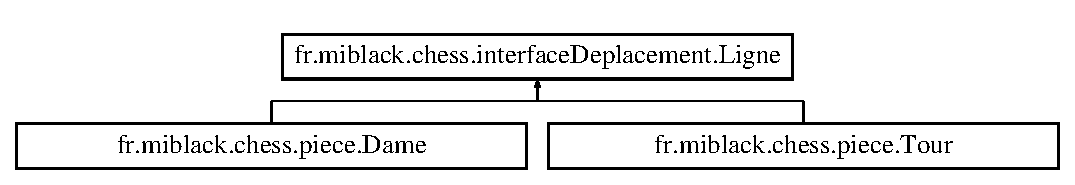
\includegraphics[height=2.000000cm]{interfacefr_1_1miblack_1_1chess_1_1interfaceDeplacement_1_1Ligne}
\end{center}
\end{figure}
\subsection*{Public Member Functions}
\begin{DoxyCompactItemize}
\item 
Linked\-List$<$ {\bf Position} $>$ {\bf position\-Ligne} ()
\end{DoxyCompactItemize}


\subsection{Detailed Description}
\begin{DoxyAuthor}{Author}
mi-\/black 
\end{DoxyAuthor}


\subsection{Member Function Documentation}
\index{fr\-::miblack\-::chess\-::interface\-Deplacement\-::\-Ligne@{fr\-::miblack\-::chess\-::interface\-Deplacement\-::\-Ligne}!position\-Ligne@{position\-Ligne}}
\index{position\-Ligne@{position\-Ligne}!fr::miblack::chess::interfaceDeplacement::Ligne@{fr\-::miblack\-::chess\-::interface\-Deplacement\-::\-Ligne}}
\subsubsection[{position\-Ligne}]{\setlength{\rightskip}{0pt plus 5cm}Linked\-List$<${\bf Position}$>$ fr.\-miblack.\-chess.\-interface\-Deplacement.\-Ligne.\-position\-Ligne (
\begin{DoxyParamCaption}
{}
\end{DoxyParamCaption}
)}\label{interfacefr_1_1miblack_1_1chess_1_1interfaceDeplacement_1_1Ligne_a55b5c0cdf05915b5996754c845591399}
\begin{DoxyReturn}{Returns}
liste des pos en ligne 
\end{DoxyReturn}


Implemented in {\bf fr.\-miblack.\-chess.\-piece.\-Dame} \doxyref{}{p.}{classfr_1_1miblack_1_1chess_1_1piece_1_1Dame_a4d2aaeb188e82f1f801e5c8311677362}, and {\bf fr.\-miblack.\-chess.\-piece.\-Tour} \doxyref{}{p.}{classfr_1_1miblack_1_1chess_1_1piece_1_1Tour_aef9cf1b642e1d24904f41d037e29f8a1}.



The documentation for this interface was generated from the following file\-:\begin{DoxyCompactItemize}
\item 
fr/miblack/chess/interface\-Deplacement/Ligne.\-java\end{DoxyCompactItemize}

\section{fr.\-miblack.\-chess.\-Main Class Reference}
\label{classfr_1_1miblack_1_1chess_1_1Main}\index{fr.\-miblack.\-chess.\-Main@{fr.\-miblack.\-chess.\-Main}}
\subsection*{Static Public Member Functions}
\begin{DoxyCompactItemize}
\item 
static void {\bf main} (String[$\,$] args)
\end{DoxyCompactItemize}


\subsection{Detailed Description}
La classe de Launch \begin{DoxyAuthor}{Author}
mi-\/black 
\end{DoxyAuthor}


\subsection{Member Function Documentation}
\index{fr\-::miblack\-::chess\-::\-Main@{fr\-::miblack\-::chess\-::\-Main}!main@{main}}
\index{main@{main}!fr::miblack::chess::Main@{fr\-::miblack\-::chess\-::\-Main}}
\subsubsection[{main}]{\setlength{\rightskip}{0pt plus 5cm}static void fr.\-miblack.\-chess.\-Main.\-main (
\begin{DoxyParamCaption}
\item[{String[$\,$]}]{args}
\end{DoxyParamCaption}
)\hspace{0.3cm}{\ttfamily [static]}}\label{classfr_1_1miblack_1_1chess_1_1Main_a58c604f913bb01eb5f24d558eb9b5e38}
La classe main 
\begin{DoxyParams}{Parameters}
{\em args} & Les parametres \-: 0 = graphique $>$1 = textuelle \\
\hline
\end{DoxyParams}


The documentation for this class was generated from the following file\-:\begin{DoxyCompactItemize}
\item 
fr/miblack/chess/Main.\-java\end{DoxyCompactItemize}

\section{fr.\-miblack.\-chess.\-affichage.\-G\-U\-I.\-Panneau\-Affichage\-Joueur Class Reference}
\label{classfr_1_1miblack_1_1chess_1_1affichage_1_1GUI_1_1PanneauAffichageJoueur}\index{fr.\-miblack.\-chess.\-affichage.\-G\-U\-I.\-Panneau\-Affichage\-Joueur@{fr.\-miblack.\-chess.\-affichage.\-G\-U\-I.\-Panneau\-Affichage\-Joueur}}


Inherits J\-Panel.

\subsection*{Public Member Functions}
\begin{DoxyCompactItemize}
\item 
{\bf Panneau\-Affichage\-Joueur} ({\bf Partie} ma\-Partie)
\item 
{\bf Partie} {\bf get\-Ma\-Partie} ()
\item 
void {\bf set\-Ma\-Partie} ({\bf Partie} ma\-Partie)
\item 
J\-Text\-Area {\bf get\-Jtext} ()
\item 
void {\bf set\-Jtext} (J\-Text\-Area jtext)
\item 
void {\bf paint\-Components} (Graphics g)
\end{DoxyCompactItemize}


\subsection{Detailed Description}
\begin{DoxyAuthor}{Author}
mi-\/black 
\end{DoxyAuthor}


\subsection{Constructor \& Destructor Documentation}
\index{fr\-::miblack\-::chess\-::affichage\-::\-G\-U\-I\-::\-Panneau\-Affichage\-Joueur@{fr\-::miblack\-::chess\-::affichage\-::\-G\-U\-I\-::\-Panneau\-Affichage\-Joueur}!Panneau\-Affichage\-Joueur@{Panneau\-Affichage\-Joueur}}
\index{Panneau\-Affichage\-Joueur@{Panneau\-Affichage\-Joueur}!fr::miblack::chess::affichage::GUI::PanneauAffichageJoueur@{fr\-::miblack\-::chess\-::affichage\-::\-G\-U\-I\-::\-Panneau\-Affichage\-Joueur}}
\subsubsection[{Panneau\-Affichage\-Joueur}]{\setlength{\rightskip}{0pt plus 5cm}fr.\-miblack.\-chess.\-affichage.\-G\-U\-I.\-Panneau\-Affichage\-Joueur.\-Panneau\-Affichage\-Joueur (
\begin{DoxyParamCaption}
\item[{{\bf Partie}}]{ma\-Partie}
\end{DoxyParamCaption}
)}\label{classfr_1_1miblack_1_1chess_1_1affichage_1_1GUI_1_1PanneauAffichageJoueur_ae2606a84306d541b0444239d56bd88b2}

\begin{DoxyParams}{Parameters}
{\em ma\-Partie} & \\
\hline
\end{DoxyParams}


\subsection{Member Function Documentation}
\index{fr\-::miblack\-::chess\-::affichage\-::\-G\-U\-I\-::\-Panneau\-Affichage\-Joueur@{fr\-::miblack\-::chess\-::affichage\-::\-G\-U\-I\-::\-Panneau\-Affichage\-Joueur}!get\-Jtext@{get\-Jtext}}
\index{get\-Jtext@{get\-Jtext}!fr::miblack::chess::affichage::GUI::PanneauAffichageJoueur@{fr\-::miblack\-::chess\-::affichage\-::\-G\-U\-I\-::\-Panneau\-Affichage\-Joueur}}
\subsubsection[{get\-Jtext}]{\setlength{\rightskip}{0pt plus 5cm}J\-Text\-Area fr.\-miblack.\-chess.\-affichage.\-G\-U\-I.\-Panneau\-Affichage\-Joueur.\-get\-Jtext (
\begin{DoxyParamCaption}
{}
\end{DoxyParamCaption}
)}\label{classfr_1_1miblack_1_1chess_1_1affichage_1_1GUI_1_1PanneauAffichageJoueur_aab3c11a6b2bc5419e7aa49c62390eac5}
\begin{DoxyReturn}{Returns}

\end{DoxyReturn}
\index{fr\-::miblack\-::chess\-::affichage\-::\-G\-U\-I\-::\-Panneau\-Affichage\-Joueur@{fr\-::miblack\-::chess\-::affichage\-::\-G\-U\-I\-::\-Panneau\-Affichage\-Joueur}!get\-Ma\-Partie@{get\-Ma\-Partie}}
\index{get\-Ma\-Partie@{get\-Ma\-Partie}!fr::miblack::chess::affichage::GUI::PanneauAffichageJoueur@{fr\-::miblack\-::chess\-::affichage\-::\-G\-U\-I\-::\-Panneau\-Affichage\-Joueur}}
\subsubsection[{get\-Ma\-Partie}]{\setlength{\rightskip}{0pt plus 5cm}{\bf Partie} fr.\-miblack.\-chess.\-affichage.\-G\-U\-I.\-Panneau\-Affichage\-Joueur.\-get\-Ma\-Partie (
\begin{DoxyParamCaption}
{}
\end{DoxyParamCaption}
)}\label{classfr_1_1miblack_1_1chess_1_1affichage_1_1GUI_1_1PanneauAffichageJoueur_ae80c0c68cc422abdbb4c958818ef9f6b}
\begin{DoxyReturn}{Returns}

\end{DoxyReturn}
\index{fr\-::miblack\-::chess\-::affichage\-::\-G\-U\-I\-::\-Panneau\-Affichage\-Joueur@{fr\-::miblack\-::chess\-::affichage\-::\-G\-U\-I\-::\-Panneau\-Affichage\-Joueur}!paint\-Components@{paint\-Components}}
\index{paint\-Components@{paint\-Components}!fr::miblack::chess::affichage::GUI::PanneauAffichageJoueur@{fr\-::miblack\-::chess\-::affichage\-::\-G\-U\-I\-::\-Panneau\-Affichage\-Joueur}}
\subsubsection[{paint\-Components}]{\setlength{\rightskip}{0pt plus 5cm}void fr.\-miblack.\-chess.\-affichage.\-G\-U\-I.\-Panneau\-Affichage\-Joueur.\-paint\-Components (
\begin{DoxyParamCaption}
\item[{Graphics}]{g}
\end{DoxyParamCaption}
)}\label{classfr_1_1miblack_1_1chess_1_1affichage_1_1GUI_1_1PanneauAffichageJoueur_a72f7a727048298dbe3ac6729fdc9ec5d}
param g \index{fr\-::miblack\-::chess\-::affichage\-::\-G\-U\-I\-::\-Panneau\-Affichage\-Joueur@{fr\-::miblack\-::chess\-::affichage\-::\-G\-U\-I\-::\-Panneau\-Affichage\-Joueur}!set\-Jtext@{set\-Jtext}}
\index{set\-Jtext@{set\-Jtext}!fr::miblack::chess::affichage::GUI::PanneauAffichageJoueur@{fr\-::miblack\-::chess\-::affichage\-::\-G\-U\-I\-::\-Panneau\-Affichage\-Joueur}}
\subsubsection[{set\-Jtext}]{\setlength{\rightskip}{0pt plus 5cm}void fr.\-miblack.\-chess.\-affichage.\-G\-U\-I.\-Panneau\-Affichage\-Joueur.\-set\-Jtext (
\begin{DoxyParamCaption}
\item[{J\-Text\-Area}]{jtext}
\end{DoxyParamCaption}
)}\label{classfr_1_1miblack_1_1chess_1_1affichage_1_1GUI_1_1PanneauAffichageJoueur_ac8afb7dc314979480347e3d3da2ab835}

\begin{DoxyParams}{Parameters}
{\em jtext} & \\
\hline
\end{DoxyParams}
\index{fr\-::miblack\-::chess\-::affichage\-::\-G\-U\-I\-::\-Panneau\-Affichage\-Joueur@{fr\-::miblack\-::chess\-::affichage\-::\-G\-U\-I\-::\-Panneau\-Affichage\-Joueur}!set\-Ma\-Partie@{set\-Ma\-Partie}}
\index{set\-Ma\-Partie@{set\-Ma\-Partie}!fr::miblack::chess::affichage::GUI::PanneauAffichageJoueur@{fr\-::miblack\-::chess\-::affichage\-::\-G\-U\-I\-::\-Panneau\-Affichage\-Joueur}}
\subsubsection[{set\-Ma\-Partie}]{\setlength{\rightskip}{0pt plus 5cm}void fr.\-miblack.\-chess.\-affichage.\-G\-U\-I.\-Panneau\-Affichage\-Joueur.\-set\-Ma\-Partie (
\begin{DoxyParamCaption}
\item[{{\bf Partie}}]{ma\-Partie}
\end{DoxyParamCaption}
)}\label{classfr_1_1miblack_1_1chess_1_1affichage_1_1GUI_1_1PanneauAffichageJoueur_a22fbdf7da577e73fc0ca0bb7028481db}

\begin{DoxyParams}{Parameters}
{\em ma\-Partie} & \\
\hline
\end{DoxyParams}


The documentation for this class was generated from the following file\-:\begin{DoxyCompactItemize}
\item 
fr/miblack/chess/affichage/\-G\-U\-I/Panneau\-Affichage\-Joueur.\-java\end{DoxyCompactItemize}

\section{fr.\-miblack.\-chess.\-Partie Class Reference}
\label{classfr_1_1miblack_1_1chess_1_1Partie}\index{fr.\-miblack.\-chess.\-Partie@{fr.\-miblack.\-chess.\-Partie}}
\subsection*{Public Member Functions}
\begin{DoxyCompactItemize}
\item 
{\bf Partie} ({\bf Joueur\-Abstract} player1, {\bf Joueur\-Abstract} player2)
\item 
{\bf Partie} {\bf clone} ()
\item 
{\bf Echiquier} {\bf get\-My\-Chessboard} ()
\item 
boolean {\bf est\-Pat} ({\bf Joueur\-Abstract} p)
\item 
boolean {\bf est\-En\-Echec} ({\bf Position} la\-Pos)
\item 
void {\bf set\-List\-Of\-Move} (Linked\-List$<$ {\bf Coup} $>$ list\-Of\-Move)
\item 
boolean {\bf sera\-En\-Echec} ({\bf Position} la\-Pos\-D, {\bf Position} la\-Pos\-A)
\item 
{\bf Position} {\bf get\-Pos\-Roi} ()
\item 
{\bf Position} {\bf get\-Pos\-Tour} (boolean petit\-Roque)
\item 
boolean {\bf trajet\-Libre} ({\bf Echiquier} chess, {\bf Position} Roi, boolean petit\-Roque)
\item 
boolean {\bf petit\-Roque\-Possible} ({\bf Echiquier} chess)
\item 
boolean {\bf grand\-Roque\-Possible} ({\bf Echiquier} chess)
\item 
boolean {\bf promotion\-Possible} ()
\item 
void {\bf realiser\-Coup} ({\bf Coup} m)
\item 
boolean {\bf est\-En\-Echec} ({\bf Joueur\-Abstract} p)
\item 
boolean {\bf est\-Echec\-Et\-Mat} ({\bf Joueur\-Abstract} p)
\item 
boolean {\bf is\-Draw} ()
\item 
void {\bf save\-Game} (String path\-Of\-File)
\item 
void {\bf load\-Game} (String path\-Of\-File, {\bf Interface} mon\-Interface)
\item 
Linked\-List$<$ {\bf Coup} $>$ {\bf list\-Of\-Available\-Move} ({\bf Joueur\-Abstract} p)
\item 
void {\bf init\-Positions} ()
\item 
void {\bf lets\-Play} ({\bf Joueur\-Abstract} joueur1)
\item 
boolean {\bf add\-Move} ({\bf Coup} e)
\item 
{\bf Joueur\-Abstract} {\bf get\-Joueur} (int i)
\item 
String {\bf mise\-En\-Forme\-List\-Coup} ()
\item 
int {\bf get\-Cpt\-\_\-sans\-\_\-prise} ()
\item 
void {\bf up\-Cpt\-\_\-sans\-\_\-prise} ()
\item 
void {\bf set\-Cpt\-\_\-sans\-\_\-prise} ()
\item 
void {\bf down\-Cpt\-\_\-sans\-\_\-prise} ()
\item 
void {\bf set\-Cpt\-Sans\-Mvmt\-Pion} ()
\item 
void {\bf up\-Cpt\-Sans\-Mvmt\-Pion} ()
\item 
{\bf Joueur\-Abstract} {\bf get\-Player\-En\-Cours} ()
\item 
void {\bf set\-Player\-En\-Cours} ()
\item 
Linked\-List$<$ {\bf Joueur\-Abstract} $>$ {\bf get\-List\-Of\-Player} ()
\item 
Linked\-List$<$ {\bf Coup} $>$ {\bf get\-List\-Of\-Move} ()
\end{DoxyCompactItemize}


\subsection{Detailed Description}
\begin{DoxyAuthor}{Author}
mi-\/black Une partie est définie par ... list\-Of\-Move \-:une liste de coup list\-Of\-Player \-: une liste de joueurs player\-En\-Cours \-: le joueur qui possède la main cpt\-\_\-sans\-\_\-prise \-: le nbre de coup sans 1 prise de piece cpt\-Sans\-Mvmt\-Pion \-: le nbre de coup dans déplacer un pion my\-Chessboard \-: l'echiquier sur lequel se base la partie 
\end{DoxyAuthor}


\subsection{Constructor \& Destructor Documentation}
\index{fr\-::miblack\-::chess\-::\-Partie@{fr\-::miblack\-::chess\-::\-Partie}!Partie@{Partie}}
\index{Partie@{Partie}!fr::miblack::chess::Partie@{fr\-::miblack\-::chess\-::\-Partie}}
\subsubsection[{Partie}]{\setlength{\rightskip}{0pt plus 5cm}fr.\-miblack.\-chess.\-Partie.\-Partie (
\begin{DoxyParamCaption}
\item[{{\bf Joueur\-Abstract}}]{player1, }
\item[{{\bf Joueur\-Abstract}}]{player2}
\end{DoxyParamCaption}
)}\label{classfr_1_1miblack_1_1chess_1_1Partie_aae0ab79f06e9db0beeabb34b8b0b9274}
Constructeur de partie 
\begin{DoxyParams}{Parameters}
{\em player1} & \\
\hline
{\em player2} & \\
\hline
\end{DoxyParams}


\subsection{Member Function Documentation}
\index{fr\-::miblack\-::chess\-::\-Partie@{fr\-::miblack\-::chess\-::\-Partie}!add\-Move@{add\-Move}}
\index{add\-Move@{add\-Move}!fr::miblack::chess::Partie@{fr\-::miblack\-::chess\-::\-Partie}}
\subsubsection[{add\-Move}]{\setlength{\rightskip}{0pt plus 5cm}boolean fr.\-miblack.\-chess.\-Partie.\-add\-Move (
\begin{DoxyParamCaption}
\item[{{\bf Coup}}]{e}
\end{DoxyParamCaption}
)}\label{classfr_1_1miblack_1_1chess_1_1Partie_a0260b2175f3ff632058ed93b8a44318c}

\begin{DoxyParams}{Parameters}
{\em e} & un coup \\
\hline
\end{DoxyParams}
\begin{DoxyReturn}{Returns}

\end{DoxyReturn}
\index{fr\-::miblack\-::chess\-::\-Partie@{fr\-::miblack\-::chess\-::\-Partie}!clone@{clone}}
\index{clone@{clone}!fr::miblack::chess::Partie@{fr\-::miblack\-::chess\-::\-Partie}}
\subsubsection[{clone}]{\setlength{\rightskip}{0pt plus 5cm}{\bf Partie} fr.\-miblack.\-chess.\-Partie.\-clone (
\begin{DoxyParamCaption}
{}
\end{DoxyParamCaption}
)}\label{classfr_1_1miblack_1_1chess_1_1Partie_a614f741d4b077fa6fc9212df602c8089}
\begin{DoxyReturn}{Returns}

\end{DoxyReturn}
\index{fr\-::miblack\-::chess\-::\-Partie@{fr\-::miblack\-::chess\-::\-Partie}!down\-Cpt\-\_\-sans\-\_\-prise@{down\-Cpt\-\_\-sans\-\_\-prise}}
\index{down\-Cpt\-\_\-sans\-\_\-prise@{down\-Cpt\-\_\-sans\-\_\-prise}!fr::miblack::chess::Partie@{fr\-::miblack\-::chess\-::\-Partie}}
\subsubsection[{down\-Cpt\-\_\-sans\-\_\-prise}]{\setlength{\rightskip}{0pt plus 5cm}void fr.\-miblack.\-chess.\-Partie.\-down\-Cpt\-\_\-sans\-\_\-prise (
\begin{DoxyParamCaption}
{}
\end{DoxyParamCaption}
)}\label{classfr_1_1miblack_1_1chess_1_1Partie_ad6a84f7041546f8fa42d459e96f9d524}
\begin{DoxyReturn}{Returns}

\end{DoxyReturn}
\index{fr\-::miblack\-::chess\-::\-Partie@{fr\-::miblack\-::chess\-::\-Partie}!est\-Echec\-Et\-Mat@{est\-Echec\-Et\-Mat}}
\index{est\-Echec\-Et\-Mat@{est\-Echec\-Et\-Mat}!fr::miblack::chess::Partie@{fr\-::miblack\-::chess\-::\-Partie}}
\subsubsection[{est\-Echec\-Et\-Mat}]{\setlength{\rightskip}{0pt plus 5cm}boolean fr.\-miblack.\-chess.\-Partie.\-est\-Echec\-Et\-Mat (
\begin{DoxyParamCaption}
\item[{{\bf Joueur\-Abstract}}]{p}
\end{DoxyParamCaption}
)}\label{classfr_1_1miblack_1_1chess_1_1Partie_ae81041ee017051a6172035d38a681690}
\begin{DoxyAuthor}{Author}
mi-\/black Cette fonction vérifie pour chaque piece si son déplacement mettera le joueur p en Echec , si c'est le cas pour tout les coups alors p est mat 
\end{DoxyAuthor}

\begin{DoxyParams}{Parameters}
{\em p} & le joueur à vérifier \\
\hline
\end{DoxyParams}
\begin{DoxyReturn}{Returns}
si le joueur p est réelement Echecs \& mat 
\end{DoxyReturn}
\index{fr\-::miblack\-::chess\-::\-Partie@{fr\-::miblack\-::chess\-::\-Partie}!est\-En\-Echec@{est\-En\-Echec}}
\index{est\-En\-Echec@{est\-En\-Echec}!fr::miblack::chess::Partie@{fr\-::miblack\-::chess\-::\-Partie}}
\subsubsection[{est\-En\-Echec}]{\setlength{\rightskip}{0pt plus 5cm}boolean fr.\-miblack.\-chess.\-Partie.\-est\-En\-Echec (
\begin{DoxyParamCaption}
\item[{{\bf Position}}]{la\-Pos}
\end{DoxyParamCaption}
)}\label{classfr_1_1miblack_1_1chess_1_1Partie_aeb8236bf742e1bc190caee47081ea146}

\begin{DoxyParams}{Parameters}
{\em la\-Pos} & la pos ou se de placer \\
\hline
\end{DoxyParams}
\begin{DoxyReturn}{Returns}
si on est en Echecs à la\-Pos 
\end{DoxyReturn}
\index{fr\-::miblack\-::chess\-::\-Partie@{fr\-::miblack\-::chess\-::\-Partie}!est\-En\-Echec@{est\-En\-Echec}}
\index{est\-En\-Echec@{est\-En\-Echec}!fr::miblack::chess::Partie@{fr\-::miblack\-::chess\-::\-Partie}}
\subsubsection[{est\-En\-Echec}]{\setlength{\rightskip}{0pt plus 5cm}boolean fr.\-miblack.\-chess.\-Partie.\-est\-En\-Echec (
\begin{DoxyParamCaption}
\item[{{\bf Joueur\-Abstract}}]{p}
\end{DoxyParamCaption}
)}\label{classfr_1_1miblack_1_1chess_1_1Partie_aa5c237b281720ebc21a3fe5d58234908}
Cette fonction vérifie si le roi de p est dans la liste de déplacement d'une des pieces de l'adversaire \begin{DoxyAuthor}{Author}
mi-\/black 
\end{DoxyAuthor}

\begin{DoxyParams}{Parameters}
{\em p} & le joueur à vérifier \\
\hline
\end{DoxyParams}
\begin{DoxyReturn}{Returns}
si le joueur p est en Echecs 
\end{DoxyReturn}
\index{fr\-::miblack\-::chess\-::\-Partie@{fr\-::miblack\-::chess\-::\-Partie}!est\-Pat@{est\-Pat}}
\index{est\-Pat@{est\-Pat}!fr::miblack::chess::Partie@{fr\-::miblack\-::chess\-::\-Partie}}
\subsubsection[{est\-Pat}]{\setlength{\rightskip}{0pt plus 5cm}boolean fr.\-miblack.\-chess.\-Partie.\-est\-Pat (
\begin{DoxyParamCaption}
\item[{{\bf Joueur\-Abstract}}]{p}
\end{DoxyParamCaption}
)}\label{classfr_1_1miblack_1_1chess_1_1Partie_aec95dd8e1705acd6546a7656a0fcc3e6}

\begin{DoxyParams}{Parameters}
{\em p} & un joueur \\
\hline
\end{DoxyParams}
\begin{DoxyReturn}{Returns}
p est pat ? 
\end{DoxyReturn}
\index{fr\-::miblack\-::chess\-::\-Partie@{fr\-::miblack\-::chess\-::\-Partie}!get\-Cpt\-\_\-sans\-\_\-prise@{get\-Cpt\-\_\-sans\-\_\-prise}}
\index{get\-Cpt\-\_\-sans\-\_\-prise@{get\-Cpt\-\_\-sans\-\_\-prise}!fr::miblack::chess::Partie@{fr\-::miblack\-::chess\-::\-Partie}}
\subsubsection[{get\-Cpt\-\_\-sans\-\_\-prise}]{\setlength{\rightskip}{0pt plus 5cm}int fr.\-miblack.\-chess.\-Partie.\-get\-Cpt\-\_\-sans\-\_\-prise (
\begin{DoxyParamCaption}
{}
\end{DoxyParamCaption}
)}\label{classfr_1_1miblack_1_1chess_1_1Partie_a5d9e63c06b95ddd8b754931703dd0802}
\begin{DoxyReturn}{Returns}

\end{DoxyReturn}
\index{fr\-::miblack\-::chess\-::\-Partie@{fr\-::miblack\-::chess\-::\-Partie}!get\-Joueur@{get\-Joueur}}
\index{get\-Joueur@{get\-Joueur}!fr::miblack::chess::Partie@{fr\-::miblack\-::chess\-::\-Partie}}
\subsubsection[{get\-Joueur}]{\setlength{\rightskip}{0pt plus 5cm}{\bf Joueur\-Abstract} fr.\-miblack.\-chess.\-Partie.\-get\-Joueur (
\begin{DoxyParamCaption}
\item[{int}]{i}
\end{DoxyParamCaption}
)}\label{classfr_1_1miblack_1_1chess_1_1Partie_a9ae173396bc76d15bf1cb19462e0b75c}

\begin{DoxyParams}{Parameters}
{\em i} & \\
\hline
\end{DoxyParams}
\begin{DoxyReturn}{Returns}

\end{DoxyReturn}
\index{fr\-::miblack\-::chess\-::\-Partie@{fr\-::miblack\-::chess\-::\-Partie}!get\-List\-Of\-Move@{get\-List\-Of\-Move}}
\index{get\-List\-Of\-Move@{get\-List\-Of\-Move}!fr::miblack::chess::Partie@{fr\-::miblack\-::chess\-::\-Partie}}
\subsubsection[{get\-List\-Of\-Move}]{\setlength{\rightskip}{0pt plus 5cm}Linked\-List$<${\bf Coup}$>$ fr.\-miblack.\-chess.\-Partie.\-get\-List\-Of\-Move (
\begin{DoxyParamCaption}
{}
\end{DoxyParamCaption}
)}\label{classfr_1_1miblack_1_1chess_1_1Partie_a17c7aadcfffcfb380c2b6d78482cc31a}
\begin{DoxyReturn}{Returns}

\end{DoxyReturn}
\index{fr\-::miblack\-::chess\-::\-Partie@{fr\-::miblack\-::chess\-::\-Partie}!get\-List\-Of\-Player@{get\-List\-Of\-Player}}
\index{get\-List\-Of\-Player@{get\-List\-Of\-Player}!fr::miblack::chess::Partie@{fr\-::miblack\-::chess\-::\-Partie}}
\subsubsection[{get\-List\-Of\-Player}]{\setlength{\rightskip}{0pt plus 5cm}Linked\-List$<${\bf Joueur\-Abstract}$>$ fr.\-miblack.\-chess.\-Partie.\-get\-List\-Of\-Player (
\begin{DoxyParamCaption}
{}
\end{DoxyParamCaption}
)}\label{classfr_1_1miblack_1_1chess_1_1Partie_a284bff812e7f1467f0440ac95ea9d7a9}
\begin{DoxyReturn}{Returns}

\end{DoxyReturn}
\index{fr\-::miblack\-::chess\-::\-Partie@{fr\-::miblack\-::chess\-::\-Partie}!get\-My\-Chessboard@{get\-My\-Chessboard}}
\index{get\-My\-Chessboard@{get\-My\-Chessboard}!fr::miblack::chess::Partie@{fr\-::miblack\-::chess\-::\-Partie}}
\subsubsection[{get\-My\-Chessboard}]{\setlength{\rightskip}{0pt plus 5cm}{\bf Echiquier} fr.\-miblack.\-chess.\-Partie.\-get\-My\-Chessboard (
\begin{DoxyParamCaption}
{}
\end{DoxyParamCaption}
)}\label{classfr_1_1miblack_1_1chess_1_1Partie_ae03ae63661645b4bd92d050a95e9ce2b}
\begin{DoxyReturn}{Returns}
my\-Chessboard 
\end{DoxyReturn}
\index{fr\-::miblack\-::chess\-::\-Partie@{fr\-::miblack\-::chess\-::\-Partie}!get\-Player\-En\-Cours@{get\-Player\-En\-Cours}}
\index{get\-Player\-En\-Cours@{get\-Player\-En\-Cours}!fr::miblack::chess::Partie@{fr\-::miblack\-::chess\-::\-Partie}}
\subsubsection[{get\-Player\-En\-Cours}]{\setlength{\rightskip}{0pt plus 5cm}{\bf Joueur\-Abstract} fr.\-miblack.\-chess.\-Partie.\-get\-Player\-En\-Cours (
\begin{DoxyParamCaption}
{}
\end{DoxyParamCaption}
)}\label{classfr_1_1miblack_1_1chess_1_1Partie_a60717616379766685cf80416bd8b6ddb}
\begin{DoxyReturn}{Returns}

\end{DoxyReturn}
\index{fr\-::miblack\-::chess\-::\-Partie@{fr\-::miblack\-::chess\-::\-Partie}!get\-Pos\-Roi@{get\-Pos\-Roi}}
\index{get\-Pos\-Roi@{get\-Pos\-Roi}!fr::miblack::chess::Partie@{fr\-::miblack\-::chess\-::\-Partie}}
\subsubsection[{get\-Pos\-Roi}]{\setlength{\rightskip}{0pt plus 5cm}{\bf Position} fr.\-miblack.\-chess.\-Partie.\-get\-Pos\-Roi (
\begin{DoxyParamCaption}
{}
\end{DoxyParamCaption}
)}\label{classfr_1_1miblack_1_1chess_1_1Partie_a9081a121faa69d7b217a8ef3aefe0764}
\begin{DoxyReturn}{Returns}
la position du Roi du joueur courant 
\end{DoxyReturn}
\index{fr\-::miblack\-::chess\-::\-Partie@{fr\-::miblack\-::chess\-::\-Partie}!get\-Pos\-Tour@{get\-Pos\-Tour}}
\index{get\-Pos\-Tour@{get\-Pos\-Tour}!fr::miblack::chess::Partie@{fr\-::miblack\-::chess\-::\-Partie}}
\subsubsection[{get\-Pos\-Tour}]{\setlength{\rightskip}{0pt plus 5cm}{\bf Position} fr.\-miblack.\-chess.\-Partie.\-get\-Pos\-Tour (
\begin{DoxyParamCaption}
\item[{boolean}]{petit\-Roque}
\end{DoxyParamCaption}
)}\label{classfr_1_1miblack_1_1chess_1_1Partie_a800eec6aecc7e524de40344d743c3240}

\begin{DoxyParams}{Parameters}
{\em petit\-Roque} & \\
\hline
\end{DoxyParams}
\begin{DoxyReturn}{Returns}
la position de la tour du joueur courant concernée par le roque 
\end{DoxyReturn}
\index{fr\-::miblack\-::chess\-::\-Partie@{fr\-::miblack\-::chess\-::\-Partie}!grand\-Roque\-Possible@{grand\-Roque\-Possible}}
\index{grand\-Roque\-Possible@{grand\-Roque\-Possible}!fr::miblack::chess::Partie@{fr\-::miblack\-::chess\-::\-Partie}}
\subsubsection[{grand\-Roque\-Possible}]{\setlength{\rightskip}{0pt plus 5cm}boolean fr.\-miblack.\-chess.\-Partie.\-grand\-Roque\-Possible (
\begin{DoxyParamCaption}
\item[{{\bf Echiquier}}]{chess}
\end{DoxyParamCaption}
)}\label{classfr_1_1miblack_1_1chess_1_1Partie_a574c3a8f41cc8f17a36d401cc559b700}

\begin{DoxyParams}{Parameters}
{\em chess} & \-: l'echiquier \\
\hline
\end{DoxyParams}
\begin{DoxyReturn}{Returns}
Le grand roque est possible ? 
\end{DoxyReturn}
\index{fr\-::miblack\-::chess\-::\-Partie@{fr\-::miblack\-::chess\-::\-Partie}!init\-Positions@{init\-Positions}}
\index{init\-Positions@{init\-Positions}!fr::miblack::chess::Partie@{fr\-::miblack\-::chess\-::\-Partie}}
\subsubsection[{init\-Positions}]{\setlength{\rightskip}{0pt plus 5cm}void fr.\-miblack.\-chess.\-Partie.\-init\-Positions (
\begin{DoxyParamCaption}
{}
\end{DoxyParamCaption}
)}\label{classfr_1_1miblack_1_1chess_1_1Partie_aa59868a6a3766d85c76fbe8a65e9527a}
Place chaque piece sur l'échiquier \begin{DoxyAuthor}{Author}
mi-\/black 
\end{DoxyAuthor}
\index{fr\-::miblack\-::chess\-::\-Partie@{fr\-::miblack\-::chess\-::\-Partie}!is\-Draw@{is\-Draw}}
\index{is\-Draw@{is\-Draw}!fr::miblack::chess::Partie@{fr\-::miblack\-::chess\-::\-Partie}}
\subsubsection[{is\-Draw}]{\setlength{\rightskip}{0pt plus 5cm}boolean fr.\-miblack.\-chess.\-Partie.\-is\-Draw (
\begin{DoxyParamCaption}
{}
\end{DoxyParamCaption}
)}\label{classfr_1_1miblack_1_1chess_1_1Partie_a38650fb7d5af87daa0676c1467e93b09}
Verifie s'il y a une partie nulle \begin{DoxyAuthor}{Author}
mi-\/black 
\end{DoxyAuthor}
\begin{DoxyReturn}{Returns}
draw , une partie est considérée comme nulle si cpt\-Sans\-Mvmt\-Pion ou cpt\-\_\-sans\-\_\-prise sont $>$50 
\end{DoxyReturn}
\index{fr\-::miblack\-::chess\-::\-Partie@{fr\-::miblack\-::chess\-::\-Partie}!lets\-Play@{lets\-Play}}
\index{lets\-Play@{lets\-Play}!fr::miblack::chess::Partie@{fr\-::miblack\-::chess\-::\-Partie}}
\subsubsection[{lets\-Play}]{\setlength{\rightskip}{0pt plus 5cm}void fr.\-miblack.\-chess.\-Partie.\-lets\-Play (
\begin{DoxyParamCaption}
\item[{{\bf Joueur\-Abstract}}]{joueur1}
\end{DoxyParamCaption}
)}\label{classfr_1_1miblack_1_1chess_1_1Partie_a9d5461bb171d95f76f386e1226db285c}
initialise les positions puis affecte le joueurs au blanc \begin{DoxyAuthor}{Author}
mi-\/black 
\end{DoxyAuthor}

\begin{DoxyParams}{Parameters}
{\em joueur1} & le joueur jouant les blancs \\
\hline
\end{DoxyParams}
\index{fr\-::miblack\-::chess\-::\-Partie@{fr\-::miblack\-::chess\-::\-Partie}!list\-Of\-Available\-Move@{list\-Of\-Available\-Move}}
\index{list\-Of\-Available\-Move@{list\-Of\-Available\-Move}!fr::miblack::chess::Partie@{fr\-::miblack\-::chess\-::\-Partie}}
\subsubsection[{list\-Of\-Available\-Move}]{\setlength{\rightskip}{0pt plus 5cm}Linked\-List$<${\bf Coup}$>$ fr.\-miblack.\-chess.\-Partie.\-list\-Of\-Available\-Move (
\begin{DoxyParamCaption}
\item[{{\bf Joueur\-Abstract}}]{p}
\end{DoxyParamCaption}
)}\label{classfr_1_1miblack_1_1chess_1_1Partie_a2055825bdb1ad2b81ea83e4a9cfd8f29}
\begin{DoxyAuthor}{Author}
mi-\/black 
\end{DoxyAuthor}

\begin{DoxyParams}{Parameters}
{\em p} & le joueur dont on veux la liste \\
\hline
\end{DoxyParams}
\begin{DoxyReturn}{Returns}
Liste des coups possibles 
\end{DoxyReturn}
\index{fr\-::miblack\-::chess\-::\-Partie@{fr\-::miblack\-::chess\-::\-Partie}!load\-Game@{load\-Game}}
\index{load\-Game@{load\-Game}!fr::miblack::chess::Partie@{fr\-::miblack\-::chess\-::\-Partie}}
\subsubsection[{load\-Game}]{\setlength{\rightskip}{0pt plus 5cm}void fr.\-miblack.\-chess.\-Partie.\-load\-Game (
\begin{DoxyParamCaption}
\item[{String}]{path\-Of\-File, }
\item[{{\bf Interface}}]{mon\-Interface}
\end{DoxyParamCaption}
)}\label{classfr_1_1miblack_1_1chess_1_1Partie_a67fa9ce7f203402e6958ec8e6383382b}
Cette fonction permet de charger une partie , elle reprend une partie de zéro et effectue chaque coups un par un \begin{DoxyAuthor}{Author}
mi-\/black 
\end{DoxyAuthor}

\begin{DoxyParams}{Parameters}
{\em path\-Of\-File} & Le fichier à charger \\
\hline
{\em mon\-Interface} & L'interface à charger \\
\hline
\end{DoxyParams}
\index{fr\-::miblack\-::chess\-::\-Partie@{fr\-::miblack\-::chess\-::\-Partie}!mise\-En\-Forme\-List\-Coup@{mise\-En\-Forme\-List\-Coup}}
\index{mise\-En\-Forme\-List\-Coup@{mise\-En\-Forme\-List\-Coup}!fr::miblack::chess::Partie@{fr\-::miblack\-::chess\-::\-Partie}}
\subsubsection[{mise\-En\-Forme\-List\-Coup}]{\setlength{\rightskip}{0pt plus 5cm}String fr.\-miblack.\-chess.\-Partie.\-mise\-En\-Forme\-List\-Coup (
\begin{DoxyParamCaption}
{}
\end{DoxyParamCaption}
)}\label{classfr_1_1miblack_1_1chess_1_1Partie_a7ee5b382b78b2b976762c791347f3d35}
met en forme la liste des coups joués pour posseder une syntaxe comme a2-\/a4 a7-\/a5 Ta1-\/a3 \begin{DoxyAuthor}{Author}
mi-\/black 
\end{DoxyAuthor}
\begin{DoxyReturn}{Returns}
la liste des coups avec une syntaxe correcte 
\end{DoxyReturn}
\index{fr\-::miblack\-::chess\-::\-Partie@{fr\-::miblack\-::chess\-::\-Partie}!petit\-Roque\-Possible@{petit\-Roque\-Possible}}
\index{petit\-Roque\-Possible@{petit\-Roque\-Possible}!fr::miblack::chess::Partie@{fr\-::miblack\-::chess\-::\-Partie}}
\subsubsection[{petit\-Roque\-Possible}]{\setlength{\rightskip}{0pt plus 5cm}boolean fr.\-miblack.\-chess.\-Partie.\-petit\-Roque\-Possible (
\begin{DoxyParamCaption}
\item[{{\bf Echiquier}}]{chess}
\end{DoxyParamCaption}
)}\label{classfr_1_1miblack_1_1chess_1_1Partie_a6ae7bfbaeccfa7790fe3dcd8c790c1a9}

\begin{DoxyParams}{Parameters}
{\em chess} & l'echiquier \\
\hline
\end{DoxyParams}
\begin{DoxyReturn}{Returns}
Le petit roque est possible ? 
\end{DoxyReturn}
\index{fr\-::miblack\-::chess\-::\-Partie@{fr\-::miblack\-::chess\-::\-Partie}!promotion\-Possible@{promotion\-Possible}}
\index{promotion\-Possible@{promotion\-Possible}!fr::miblack::chess::Partie@{fr\-::miblack\-::chess\-::\-Partie}}
\subsubsection[{promotion\-Possible}]{\setlength{\rightskip}{0pt plus 5cm}boolean fr.\-miblack.\-chess.\-Partie.\-promotion\-Possible (
\begin{DoxyParamCaption}
{}
\end{DoxyParamCaption}
)}\label{classfr_1_1miblack_1_1chess_1_1Partie_a27612ab3eb4a9b64a792357c61b5d129}
Verifie si une promotion est possible \begin{DoxyAuthor}{Author}
mi-\/black 
\end{DoxyAuthor}
\begin{DoxyReturn}{Returns}

\end{DoxyReturn}
\index{fr\-::miblack\-::chess\-::\-Partie@{fr\-::miblack\-::chess\-::\-Partie}!realiser\-Coup@{realiser\-Coup}}
\index{realiser\-Coup@{realiser\-Coup}!fr::miblack::chess::Partie@{fr\-::miblack\-::chess\-::\-Partie}}
\subsubsection[{realiser\-Coup}]{\setlength{\rightskip}{0pt plus 5cm}void fr.\-miblack.\-chess.\-Partie.\-realiser\-Coup (
\begin{DoxyParamCaption}
\item[{{\bf Coup}}]{m}
\end{DoxyParamCaption}
)}\label{classfr_1_1miblack_1_1chess_1_1Partie_a54371190badace613e8028e2f15e4088}
augmente les compteurs de partie nulle puis réalise un coup sur l'échiquier et ajoute enfin le coup à la liste des coups 
\begin{DoxyParams}{Parameters}
{\em m} & le coup à réaliser \\
\hline
\end{DoxyParams}
\index{fr\-::miblack\-::chess\-::\-Partie@{fr\-::miblack\-::chess\-::\-Partie}!save\-Game@{save\-Game}}
\index{save\-Game@{save\-Game}!fr::miblack::chess::Partie@{fr\-::miblack\-::chess\-::\-Partie}}
\subsubsection[{save\-Game}]{\setlength{\rightskip}{0pt plus 5cm}void fr.\-miblack.\-chess.\-Partie.\-save\-Game (
\begin{DoxyParamCaption}
\item[{String}]{path\-Of\-File}
\end{DoxyParamCaption}
)}\label{classfr_1_1miblack_1_1chess_1_1Partie_ab52cf6d86b2e76e462620c09ab69adbb}
Cette fonction permet donc d'enregistrer une partie dans un fichier texte \begin{DoxyAuthor}{Author}
mi-\/black 
\end{DoxyAuthor}

\begin{DoxyParams}{Parameters}
{\em path\-Of\-File} & Le fichier où sauvegarder \\
\hline
\end{DoxyParams}
\index{fr\-::miblack\-::chess\-::\-Partie@{fr\-::miblack\-::chess\-::\-Partie}!sera\-En\-Echec@{sera\-En\-Echec}}
\index{sera\-En\-Echec@{sera\-En\-Echec}!fr::miblack::chess::Partie@{fr\-::miblack\-::chess\-::\-Partie}}
\subsubsection[{sera\-En\-Echec}]{\setlength{\rightskip}{0pt plus 5cm}boolean fr.\-miblack.\-chess.\-Partie.\-sera\-En\-Echec (
\begin{DoxyParamCaption}
\item[{{\bf Position}}]{la\-Pos\-D, }
\item[{{\bf Position}}]{la\-Pos\-A}
\end{DoxyParamCaption}
)}\label{classfr_1_1miblack_1_1chess_1_1Partie_a40ebcd05ee064686fc1dfe84d826e9ea}
Verifie si l'on est en echec si l'on bouge une piece d'une pos\-D à une pos\-A 
\begin{DoxyParams}{Parameters}
{\em la\-Pos\-D} & \\
\hline
{\em la\-Pos\-A} & \\
\hline
\end{DoxyParams}
\begin{DoxyReturn}{Returns}
si pos\-D se libere et que la piece va en pos\-A , y aura echec ? 
\end{DoxyReturn}
\index{fr\-::miblack\-::chess\-::\-Partie@{fr\-::miblack\-::chess\-::\-Partie}!set\-Cpt\-\_\-sans\-\_\-prise@{set\-Cpt\-\_\-sans\-\_\-prise}}
\index{set\-Cpt\-\_\-sans\-\_\-prise@{set\-Cpt\-\_\-sans\-\_\-prise}!fr::miblack::chess::Partie@{fr\-::miblack\-::chess\-::\-Partie}}
\subsubsection[{set\-Cpt\-\_\-sans\-\_\-prise}]{\setlength{\rightskip}{0pt plus 5cm}void fr.\-miblack.\-chess.\-Partie.\-set\-Cpt\-\_\-sans\-\_\-prise (
\begin{DoxyParamCaption}
{}
\end{DoxyParamCaption}
)}\label{classfr_1_1miblack_1_1chess_1_1Partie_a75c7c35eb2d94d8793644670b7ac4f38}
\begin{DoxyReturn}{Returns}

\end{DoxyReturn}
\index{fr\-::miblack\-::chess\-::\-Partie@{fr\-::miblack\-::chess\-::\-Partie}!set\-Cpt\-Sans\-Mvmt\-Pion@{set\-Cpt\-Sans\-Mvmt\-Pion}}
\index{set\-Cpt\-Sans\-Mvmt\-Pion@{set\-Cpt\-Sans\-Mvmt\-Pion}!fr::miblack::chess::Partie@{fr\-::miblack\-::chess\-::\-Partie}}
\subsubsection[{set\-Cpt\-Sans\-Mvmt\-Pion}]{\setlength{\rightskip}{0pt plus 5cm}void fr.\-miblack.\-chess.\-Partie.\-set\-Cpt\-Sans\-Mvmt\-Pion (
\begin{DoxyParamCaption}
{}
\end{DoxyParamCaption}
)}\label{classfr_1_1miblack_1_1chess_1_1Partie_a805df7c45719eb765e1ca3f3addcfac1}
\begin{DoxyReturn}{Returns}

\end{DoxyReturn}
\index{fr\-::miblack\-::chess\-::\-Partie@{fr\-::miblack\-::chess\-::\-Partie}!set\-List\-Of\-Move@{set\-List\-Of\-Move}}
\index{set\-List\-Of\-Move@{set\-List\-Of\-Move}!fr::miblack::chess::Partie@{fr\-::miblack\-::chess\-::\-Partie}}
\subsubsection[{set\-List\-Of\-Move}]{\setlength{\rightskip}{0pt plus 5cm}void fr.\-miblack.\-chess.\-Partie.\-set\-List\-Of\-Move (
\begin{DoxyParamCaption}
\item[{Linked\-List$<$ {\bf Coup} $>$}]{list\-Of\-Move}
\end{DoxyParamCaption}
)}\label{classfr_1_1miblack_1_1chess_1_1Partie_a56b250bd48deeddcfbd0c993dfc6b22f}

\begin{DoxyParams}{Parameters}
{\em list\-Of\-Move} & \\
\hline
\end{DoxyParams}
\index{fr\-::miblack\-::chess\-::\-Partie@{fr\-::miblack\-::chess\-::\-Partie}!set\-Player\-En\-Cours@{set\-Player\-En\-Cours}}
\index{set\-Player\-En\-Cours@{set\-Player\-En\-Cours}!fr::miblack::chess::Partie@{fr\-::miblack\-::chess\-::\-Partie}}
\subsubsection[{set\-Player\-En\-Cours}]{\setlength{\rightskip}{0pt plus 5cm}void fr.\-miblack.\-chess.\-Partie.\-set\-Player\-En\-Cours (
\begin{DoxyParamCaption}
{}
\end{DoxyParamCaption}
)}\label{classfr_1_1miblack_1_1chess_1_1Partie_a7bce7c2629ff6fe43042d2510bac653f}
Change le joueur en cours \begin{DoxyAuthor}{Author}
mi-\/black 
\end{DoxyAuthor}
\index{fr\-::miblack\-::chess\-::\-Partie@{fr\-::miblack\-::chess\-::\-Partie}!trajet\-Libre@{trajet\-Libre}}
\index{trajet\-Libre@{trajet\-Libre}!fr::miblack::chess::Partie@{fr\-::miblack\-::chess\-::\-Partie}}
\subsubsection[{trajet\-Libre}]{\setlength{\rightskip}{0pt plus 5cm}boolean fr.\-miblack.\-chess.\-Partie.\-trajet\-Libre (
\begin{DoxyParamCaption}
\item[{{\bf Echiquier}}]{chess, }
\item[{{\bf Position}}]{Roi, }
\item[{boolean}]{petit\-Roque}
\end{DoxyParamCaption}
)}\label{classfr_1_1miblack_1_1chess_1_1Partie_aa851c80dc1f060fe6c8e15f60bdd33d1}

\begin{DoxyParams}{Parameters}
{\em chess} & \-: l'echiquier \\
\hline
{\em Roi} & la position du roi \\
\hline
{\em petit\-Roque} & \\
\hline
\end{DoxyParams}
\begin{DoxyReturn}{Returns}
Si le trajet est possible entre le roi et le petit(ou grand) roque 
\end{DoxyReturn}
\index{fr\-::miblack\-::chess\-::\-Partie@{fr\-::miblack\-::chess\-::\-Partie}!up\-Cpt\-\_\-sans\-\_\-prise@{up\-Cpt\-\_\-sans\-\_\-prise}}
\index{up\-Cpt\-\_\-sans\-\_\-prise@{up\-Cpt\-\_\-sans\-\_\-prise}!fr::miblack::chess::Partie@{fr\-::miblack\-::chess\-::\-Partie}}
\subsubsection[{up\-Cpt\-\_\-sans\-\_\-prise}]{\setlength{\rightskip}{0pt plus 5cm}void fr.\-miblack.\-chess.\-Partie.\-up\-Cpt\-\_\-sans\-\_\-prise (
\begin{DoxyParamCaption}
{}
\end{DoxyParamCaption}
)}\label{classfr_1_1miblack_1_1chess_1_1Partie_aefa51d77b5014414e456f001c49fdd13}
\begin{DoxyReturn}{Returns}

\end{DoxyReturn}
\index{fr\-::miblack\-::chess\-::\-Partie@{fr\-::miblack\-::chess\-::\-Partie}!up\-Cpt\-Sans\-Mvmt\-Pion@{up\-Cpt\-Sans\-Mvmt\-Pion}}
\index{up\-Cpt\-Sans\-Mvmt\-Pion@{up\-Cpt\-Sans\-Mvmt\-Pion}!fr::miblack::chess::Partie@{fr\-::miblack\-::chess\-::\-Partie}}
\subsubsection[{up\-Cpt\-Sans\-Mvmt\-Pion}]{\setlength{\rightskip}{0pt plus 5cm}void fr.\-miblack.\-chess.\-Partie.\-up\-Cpt\-Sans\-Mvmt\-Pion (
\begin{DoxyParamCaption}
{}
\end{DoxyParamCaption}
)}\label{classfr_1_1miblack_1_1chess_1_1Partie_a876344260a5933bbb27384c72fb453b3}
\begin{DoxyReturn}{Returns}

\end{DoxyReturn}


The documentation for this class was generated from the following file\-:\begin{DoxyCompactItemize}
\item 
fr/miblack/chess/Partie.\-java\end{DoxyCompactItemize}

\section{fr.\-miblack.\-chess.\-piece.\-Piece Class Reference}
\label{classfr_1_1miblack_1_1chess_1_1piece_1_1Piece}\index{fr.\-miblack.\-chess.\-piece.\-Piece@{fr.\-miblack.\-chess.\-piece.\-Piece}}
Inheritance diagram for fr.\-miblack.\-chess.\-piece.\-Piece\-:\begin{figure}[H]
\begin{center}
\leavevmode
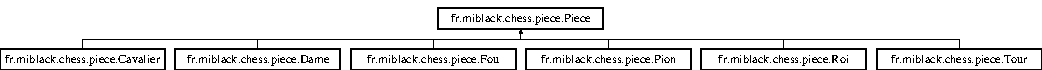
\includegraphics[height=0.938023cm]{classfr_1_1miblack_1_1chess_1_1piece_1_1Piece}
\end{center}
\end{figure}
\subsection*{Public Member Functions}
\begin{DoxyCompactItemize}
\item 
{\bf Piece} ({\bf Couleur} {\bf color}, {\bf Position} {\bf pos}, int {\bf valeur})
\item 
{\bf Couleur} {\bf get\-Color} ()
\item 
void {\bf set\-Color} (int {\bf color})
\item 
int {\bf get\-Played} ()
\item 
void {\bf set\-Played} ()
\item 
void {\bf un\-Set\-Played} ()
\item 
void {\bf set\-Pos} ({\bf Position} {\bf pos})
\item 
void {\bf set\-Pos} (int x, int y)
\item 
{\bf Position} {\bf get\-Pos} ()
\item 
int {\bf get\-Valeur} ()
\item 
abstract Linked\-List$<$ {\bf Position} $>$ {\bf position\-Accessible} ()
\item 
abstract Linked\-List$<$ {\bf Position} $>$ {\bf position\-Accessible\-Chessboard} ({\bf Echiquier} chess)
\item 
abstract Linked\-List$<$ {\bf Position} $>$ {\bf what\-Can\-I\-Eat} ({\bf Echiquier} chess)
\item 
int {\bf get\-Y} ()
\item 
int {\bf get\-X} ()
\item 
boolean {\bf est\-Valide} (int x)
\item 
boolean {\bf verif\-Color} ({\bf Echiquier} chess, {\bf Position} one\-Pos)
\item 
boolean {\bf verif\-Color} ({\bf Echiquier} chess, int x, int y)
\item 
String {\bf get\-Nom} ()
\item 
Linked\-List$<$ {\bf Coup} $>$ {\bf get\-Coup\-Possible} ({\bf Piece} Piece\-Depart, {\bf Partie} ma\-Partie)
\item 
boolean {\bf equals} ({\bf Piece} autre)
\end{DoxyCompactItemize}
\subsection*{Protected Attributes}
\begin{DoxyCompactItemize}
\item 
{\bf Couleur} {\bf color}
\item 
{\bf Position} {\bf pos}
\item 
int {\bf valeur}
\item 
int {\bf as\-Played} = 0
\end{DoxyCompactItemize}


\subsection{Detailed Description}
\begin{DoxyAuthor}{Author}
mi-\/black 
\end{DoxyAuthor}


\subsection{Constructor \& Destructor Documentation}
\index{fr\-::miblack\-::chess\-::piece\-::\-Piece@{fr\-::miblack\-::chess\-::piece\-::\-Piece}!Piece@{Piece}}
\index{Piece@{Piece}!fr::miblack::chess::piece::Piece@{fr\-::miblack\-::chess\-::piece\-::\-Piece}}
\subsubsection[{Piece}]{\setlength{\rightskip}{0pt plus 5cm}fr.\-miblack.\-chess.\-piece.\-Piece.\-Piece (
\begin{DoxyParamCaption}
\item[{{\bf Couleur}}]{color, }
\item[{{\bf Position}}]{pos, }
\item[{int}]{valeur}
\end{DoxyParamCaption}
)}\label{classfr_1_1miblack_1_1chess_1_1piece_1_1Piece_a599465960a009ce31e418d1fd8dc6701}

\begin{DoxyParams}{Parameters}
{\em color} & \\
\hline
{\em pos} & \\
\hline
{\em valeur} & \\
\hline
\end{DoxyParams}


\subsection{Member Function Documentation}
\index{fr\-::miblack\-::chess\-::piece\-::\-Piece@{fr\-::miblack\-::chess\-::piece\-::\-Piece}!equals@{equals}}
\index{equals@{equals}!fr::miblack::chess::piece::Piece@{fr\-::miblack\-::chess\-::piece\-::\-Piece}}
\subsubsection[{equals}]{\setlength{\rightskip}{0pt plus 5cm}boolean fr.\-miblack.\-chess.\-piece.\-Piece.\-equals (
\begin{DoxyParamCaption}
\item[{{\bf Piece}}]{autre}
\end{DoxyParamCaption}
)}\label{classfr_1_1miblack_1_1chess_1_1piece_1_1Piece_a2734fcebeb40ed0bd2960264330c13d9}

\begin{DoxyParams}{Parameters}
{\em autre} & \\
\hline
\end{DoxyParams}
\begin{DoxyReturn}{Returns}

\end{DoxyReturn}
\index{fr\-::miblack\-::chess\-::piece\-::\-Piece@{fr\-::miblack\-::chess\-::piece\-::\-Piece}!est\-Valide@{est\-Valide}}
\index{est\-Valide@{est\-Valide}!fr::miblack::chess::piece::Piece@{fr\-::miblack\-::chess\-::piece\-::\-Piece}}
\subsubsection[{est\-Valide}]{\setlength{\rightskip}{0pt plus 5cm}boolean fr.\-miblack.\-chess.\-piece.\-Piece.\-est\-Valide (
\begin{DoxyParamCaption}
\item[{int}]{x}
\end{DoxyParamCaption}
)}\label{classfr_1_1miblack_1_1chess_1_1piece_1_1Piece_ab76e28fdddb07543b0142450ca865b6d}

\begin{DoxyParams}{Parameters}
{\em x} & \\
\hline
\end{DoxyParams}
\begin{DoxyReturn}{Returns}

\end{DoxyReturn}
\index{fr\-::miblack\-::chess\-::piece\-::\-Piece@{fr\-::miblack\-::chess\-::piece\-::\-Piece}!get\-Color@{get\-Color}}
\index{get\-Color@{get\-Color}!fr::miblack::chess::piece::Piece@{fr\-::miblack\-::chess\-::piece\-::\-Piece}}
\subsubsection[{get\-Color}]{\setlength{\rightskip}{0pt plus 5cm}{\bf Couleur} fr.\-miblack.\-chess.\-piece.\-Piece.\-get\-Color (
\begin{DoxyParamCaption}
{}
\end{DoxyParamCaption}
)}\label{classfr_1_1miblack_1_1chess_1_1piece_1_1Piece_af4b9ae158c7008c6f6c295d1ed3e128f}
\begin{DoxyReturn}{Returns}

\end{DoxyReturn}
\index{fr\-::miblack\-::chess\-::piece\-::\-Piece@{fr\-::miblack\-::chess\-::piece\-::\-Piece}!get\-Coup\-Possible@{get\-Coup\-Possible}}
\index{get\-Coup\-Possible@{get\-Coup\-Possible}!fr::miblack::chess::piece::Piece@{fr\-::miblack\-::chess\-::piece\-::\-Piece}}
\subsubsection[{get\-Coup\-Possible}]{\setlength{\rightskip}{0pt plus 5cm}Linked\-List$<${\bf Coup}$>$ fr.\-miblack.\-chess.\-piece.\-Piece.\-get\-Coup\-Possible (
\begin{DoxyParamCaption}
\item[{{\bf Piece}}]{Piece\-Depart, }
\item[{{\bf Partie}}]{ma\-Partie}
\end{DoxyParamCaption}
)}\label{classfr_1_1miblack_1_1chess_1_1piece_1_1Piece_ace5ed8c4d7f922076255d5aa0733e51e}

\begin{DoxyParams}{Parameters}
{\em Piece\-Depart} & \\
\hline
{\em ma\-Partie} & \\
\hline
\end{DoxyParams}
\begin{DoxyReturn}{Returns}

\end{DoxyReturn}


Reimplemented in {\bf fr.\-miblack.\-chess.\-piece.\-Pion} \doxyref{}{p.}{classfr_1_1miblack_1_1chess_1_1piece_1_1Pion_a0480e38f7b6f027b01da4bef00f6f3f2}.

\index{fr\-::miblack\-::chess\-::piece\-::\-Piece@{fr\-::miblack\-::chess\-::piece\-::\-Piece}!get\-Nom@{get\-Nom}}
\index{get\-Nom@{get\-Nom}!fr::miblack::chess::piece::Piece@{fr\-::miblack\-::chess\-::piece\-::\-Piece}}
\subsubsection[{get\-Nom}]{\setlength{\rightskip}{0pt plus 5cm}String fr.\-miblack.\-chess.\-piece.\-Piece.\-get\-Nom (
\begin{DoxyParamCaption}
{}
\end{DoxyParamCaption}
)}\label{classfr_1_1miblack_1_1chess_1_1piece_1_1Piece_a68bb44429e21b7f64511a91a0861dde4}
\begin{DoxyReturn}{Returns}

\end{DoxyReturn}


Reimplemented in {\bf fr.\-miblack.\-chess.\-piece.\-Pion} \doxyref{}{p.}{classfr_1_1miblack_1_1chess_1_1piece_1_1Pion_a6a0712e0005efb52ae3ccf7b96be4957}, {\bf fr.\-miblack.\-chess.\-piece.\-Tour} \doxyref{}{p.}{classfr_1_1miblack_1_1chess_1_1piece_1_1Tour_a80e9e4055be5dadc948b3e8ec9bf22a5}, {\bf fr.\-miblack.\-chess.\-piece.\-Fou} \doxyref{}{p.}{classfr_1_1miblack_1_1chess_1_1piece_1_1Fou_ab925ec7e8e1e1765b9068ecd316f8018}, {\bf fr.\-miblack.\-chess.\-piece.\-Cavalier} \doxyref{}{p.}{classfr_1_1miblack_1_1chess_1_1piece_1_1Cavalier_a5244f4725912a3b6b6e610d9757a68e0}, {\bf fr.\-miblack.\-chess.\-piece.\-Roi} \doxyref{}{p.}{classfr_1_1miblack_1_1chess_1_1piece_1_1Roi_ae42ca462315ecdfd651c66a126cea358}, and {\bf fr.\-miblack.\-chess.\-piece.\-Dame} \doxyref{}{p.}{classfr_1_1miblack_1_1chess_1_1piece_1_1Dame_a4d16e6c8afc12ee3962905947f4fba00}.

\index{fr\-::miblack\-::chess\-::piece\-::\-Piece@{fr\-::miblack\-::chess\-::piece\-::\-Piece}!get\-Played@{get\-Played}}
\index{get\-Played@{get\-Played}!fr::miblack::chess::piece::Piece@{fr\-::miblack\-::chess\-::piece\-::\-Piece}}
\subsubsection[{get\-Played}]{\setlength{\rightskip}{0pt plus 5cm}int fr.\-miblack.\-chess.\-piece.\-Piece.\-get\-Played (
\begin{DoxyParamCaption}
{}
\end{DoxyParamCaption}
)}\label{classfr_1_1miblack_1_1chess_1_1piece_1_1Piece_aa0a7d12150182ab9ca0e5f18542d68b4}
\begin{DoxyReturn}{Returns}

\end{DoxyReturn}
\index{fr\-::miblack\-::chess\-::piece\-::\-Piece@{fr\-::miblack\-::chess\-::piece\-::\-Piece}!get\-Pos@{get\-Pos}}
\index{get\-Pos@{get\-Pos}!fr::miblack::chess::piece::Piece@{fr\-::miblack\-::chess\-::piece\-::\-Piece}}
\subsubsection[{get\-Pos}]{\setlength{\rightskip}{0pt plus 5cm}{\bf Position} fr.\-miblack.\-chess.\-piece.\-Piece.\-get\-Pos (
\begin{DoxyParamCaption}
{}
\end{DoxyParamCaption}
)}\label{classfr_1_1miblack_1_1chess_1_1piece_1_1Piece_a0332d6385641e98c16cf7775be3a621e}
\begin{DoxyReturn}{Returns}

\end{DoxyReturn}
\index{fr\-::miblack\-::chess\-::piece\-::\-Piece@{fr\-::miblack\-::chess\-::piece\-::\-Piece}!get\-Valeur@{get\-Valeur}}
\index{get\-Valeur@{get\-Valeur}!fr::miblack::chess::piece::Piece@{fr\-::miblack\-::chess\-::piece\-::\-Piece}}
\subsubsection[{get\-Valeur}]{\setlength{\rightskip}{0pt plus 5cm}int fr.\-miblack.\-chess.\-piece.\-Piece.\-get\-Valeur (
\begin{DoxyParamCaption}
{}
\end{DoxyParamCaption}
)}\label{classfr_1_1miblack_1_1chess_1_1piece_1_1Piece_ab46c5a8d83657fc3494caa0dff079673}
\begin{DoxyReturn}{Returns}

\end{DoxyReturn}
\index{fr\-::miblack\-::chess\-::piece\-::\-Piece@{fr\-::miblack\-::chess\-::piece\-::\-Piece}!get\-X@{get\-X}}
\index{get\-X@{get\-X}!fr::miblack::chess::piece::Piece@{fr\-::miblack\-::chess\-::piece\-::\-Piece}}
\subsubsection[{get\-X}]{\setlength{\rightskip}{0pt plus 5cm}int fr.\-miblack.\-chess.\-piece.\-Piece.\-get\-X (
\begin{DoxyParamCaption}
{}
\end{DoxyParamCaption}
)}\label{classfr_1_1miblack_1_1chess_1_1piece_1_1Piece_aa4f681128cf40c505c341647e58e2db9}
\begin{DoxyReturn}{Returns}

\end{DoxyReturn}
\index{fr\-::miblack\-::chess\-::piece\-::\-Piece@{fr\-::miblack\-::chess\-::piece\-::\-Piece}!get\-Y@{get\-Y}}
\index{get\-Y@{get\-Y}!fr::miblack::chess::piece::Piece@{fr\-::miblack\-::chess\-::piece\-::\-Piece}}
\subsubsection[{get\-Y}]{\setlength{\rightskip}{0pt plus 5cm}int fr.\-miblack.\-chess.\-piece.\-Piece.\-get\-Y (
\begin{DoxyParamCaption}
{}
\end{DoxyParamCaption}
)}\label{classfr_1_1miblack_1_1chess_1_1piece_1_1Piece_aba2fd4b64da2ee4a1fdd323901f383ea}
\begin{DoxyReturn}{Returns}

\end{DoxyReturn}
\index{fr\-::miblack\-::chess\-::piece\-::\-Piece@{fr\-::miblack\-::chess\-::piece\-::\-Piece}!position\-Accessible@{position\-Accessible}}
\index{position\-Accessible@{position\-Accessible}!fr::miblack::chess::piece::Piece@{fr\-::miblack\-::chess\-::piece\-::\-Piece}}
\subsubsection[{position\-Accessible}]{\setlength{\rightskip}{0pt plus 5cm}abstract Linked\-List$<${\bf Position}$>$ fr.\-miblack.\-chess.\-piece.\-Piece.\-position\-Accessible (
\begin{DoxyParamCaption}
{}
\end{DoxyParamCaption}
)\hspace{0.3cm}{\ttfamily [pure virtual]}}\label{classfr_1_1miblack_1_1chess_1_1piece_1_1Piece_ad5cdbd635ec706f16d57dccf1b8c456e}
\begin{DoxyReturn}{Returns}
List of position where one piece can be going 
\end{DoxyReturn}


Implemented in {\bf fr.\-miblack.\-chess.\-piece.\-Pion} \doxyref{}{p.}{classfr_1_1miblack_1_1chess_1_1piece_1_1Pion_ad781b079c949af93e742badb99a47608}, {\bf fr.\-miblack.\-chess.\-piece.\-Dame} \doxyref{}{p.}{classfr_1_1miblack_1_1chess_1_1piece_1_1Dame_ac25901344ee4e07425d9e3704cd22802}, {\bf fr.\-miblack.\-chess.\-piece.\-Cavalier} \doxyref{}{p.}{classfr_1_1miblack_1_1chess_1_1piece_1_1Cavalier_ab851e7c8f792c86df2d4e1c3f7448428}, {\bf fr.\-miblack.\-chess.\-piece.\-Tour} \doxyref{}{p.}{classfr_1_1miblack_1_1chess_1_1piece_1_1Tour_af607119bd40627dd4f05f6996f598094}, {\bf fr.\-miblack.\-chess.\-piece.\-Fou} \doxyref{}{p.}{classfr_1_1miblack_1_1chess_1_1piece_1_1Fou_ad3e65280fc7f9bfba09054f2a12acb34}, and {\bf fr.\-miblack.\-chess.\-piece.\-Roi} \doxyref{}{p.}{classfr_1_1miblack_1_1chess_1_1piece_1_1Roi_aafff669d094d5adcc5b8e7e79563d6c5}.

\index{fr\-::miblack\-::chess\-::piece\-::\-Piece@{fr\-::miblack\-::chess\-::piece\-::\-Piece}!position\-Accessible\-Chessboard@{position\-Accessible\-Chessboard}}
\index{position\-Accessible\-Chessboard@{position\-Accessible\-Chessboard}!fr::miblack::chess::piece::Piece@{fr\-::miblack\-::chess\-::piece\-::\-Piece}}
\subsubsection[{position\-Accessible\-Chessboard}]{\setlength{\rightskip}{0pt plus 5cm}abstract Linked\-List$<${\bf Position}$>$ fr.\-miblack.\-chess.\-piece.\-Piece.\-position\-Accessible\-Chessboard (
\begin{DoxyParamCaption}
\item[{{\bf Echiquier}}]{chess}
\end{DoxyParamCaption}
)\hspace{0.3cm}{\ttfamily [pure virtual]}}\label{classfr_1_1miblack_1_1chess_1_1piece_1_1Piece_ac1222bad9bf13533eecec2b8d99e24c6}
\begin{DoxyReturn}{Returns}
List of position where one piece can be going with restriction of the chessboard 
\end{DoxyReturn}


Implemented in {\bf fr.\-miblack.\-chess.\-piece.\-Pion} \doxyref{}{p.}{classfr_1_1miblack_1_1chess_1_1piece_1_1Pion_afd1ccbe76aef6117fd63b985913c3a10}, {\bf fr.\-miblack.\-chess.\-piece.\-Cavalier} \doxyref{}{p.}{classfr_1_1miblack_1_1chess_1_1piece_1_1Cavalier_a99eaa1d56a1f687c113116ec12e1ecb4}, {\bf fr.\-miblack.\-chess.\-piece.\-Fou} \doxyref{}{p.}{classfr_1_1miblack_1_1chess_1_1piece_1_1Fou_a9cdc9221f86c92871cb8ff54ec13843c}, {\bf fr.\-miblack.\-chess.\-piece.\-Tour} \doxyref{}{p.}{classfr_1_1miblack_1_1chess_1_1piece_1_1Tour_a68469e2ef16437fe17b81a032d21f83d}, {\bf fr.\-miblack.\-chess.\-piece.\-Roi} \doxyref{}{p.}{classfr_1_1miblack_1_1chess_1_1piece_1_1Roi_ad6fac5991349c7580cee1726d410a149}, and {\bf fr.\-miblack.\-chess.\-piece.\-Dame} \doxyref{}{p.}{classfr_1_1miblack_1_1chess_1_1piece_1_1Dame_a9b0273eab6398694c36cd5a52d985801}.

\index{fr\-::miblack\-::chess\-::piece\-::\-Piece@{fr\-::miblack\-::chess\-::piece\-::\-Piece}!set\-Color@{set\-Color}}
\index{set\-Color@{set\-Color}!fr::miblack::chess::piece::Piece@{fr\-::miblack\-::chess\-::piece\-::\-Piece}}
\subsubsection[{set\-Color}]{\setlength{\rightskip}{0pt plus 5cm}void fr.\-miblack.\-chess.\-piece.\-Piece.\-set\-Color (
\begin{DoxyParamCaption}
\item[{int}]{color}
\end{DoxyParamCaption}
)}\label{classfr_1_1miblack_1_1chess_1_1piece_1_1Piece_a7185598e9dbdc51c08c08eb6fecd432e}

\begin{DoxyParams}{Parameters}
{\em color} & \\
\hline
\end{DoxyParams}
\index{fr\-::miblack\-::chess\-::piece\-::\-Piece@{fr\-::miblack\-::chess\-::piece\-::\-Piece}!set\-Played@{set\-Played}}
\index{set\-Played@{set\-Played}!fr::miblack::chess::piece::Piece@{fr\-::miblack\-::chess\-::piece\-::\-Piece}}
\subsubsection[{set\-Played}]{\setlength{\rightskip}{0pt plus 5cm}void fr.\-miblack.\-chess.\-piece.\-Piece.\-set\-Played (
\begin{DoxyParamCaption}
{}
\end{DoxyParamCaption}
)}\label{classfr_1_1miblack_1_1chess_1_1piece_1_1Piece_af2e2bce56fe5bf4938732fcf23572bb8}
Rien \index{fr\-::miblack\-::chess\-::piece\-::\-Piece@{fr\-::miblack\-::chess\-::piece\-::\-Piece}!set\-Pos@{set\-Pos}}
\index{set\-Pos@{set\-Pos}!fr::miblack::chess::piece::Piece@{fr\-::miblack\-::chess\-::piece\-::\-Piece}}
\subsubsection[{set\-Pos}]{\setlength{\rightskip}{0pt plus 5cm}void fr.\-miblack.\-chess.\-piece.\-Piece.\-set\-Pos (
\begin{DoxyParamCaption}
\item[{{\bf Position}}]{pos}
\end{DoxyParamCaption}
)}\label{classfr_1_1miblack_1_1chess_1_1piece_1_1Piece_a830a6927a549ae1dcf6119a23c6bfdb4}

\begin{DoxyParams}{Parameters}
{\em pos} & \\
\hline
\end{DoxyParams}
\index{fr\-::miblack\-::chess\-::piece\-::\-Piece@{fr\-::miblack\-::chess\-::piece\-::\-Piece}!set\-Pos@{set\-Pos}}
\index{set\-Pos@{set\-Pos}!fr::miblack::chess::piece::Piece@{fr\-::miblack\-::chess\-::piece\-::\-Piece}}
\subsubsection[{set\-Pos}]{\setlength{\rightskip}{0pt plus 5cm}void fr.\-miblack.\-chess.\-piece.\-Piece.\-set\-Pos (
\begin{DoxyParamCaption}
\item[{int}]{x, }
\item[{int}]{y}
\end{DoxyParamCaption}
)}\label{classfr_1_1miblack_1_1chess_1_1piece_1_1Piece_a2a2d8b8bd0c09465dbff5585d4f6dd8d}

\begin{DoxyParams}{Parameters}
{\em x} & \\
\hline
{\em y} & \\
\hline
\end{DoxyParams}
\index{fr\-::miblack\-::chess\-::piece\-::\-Piece@{fr\-::miblack\-::chess\-::piece\-::\-Piece}!un\-Set\-Played@{un\-Set\-Played}}
\index{un\-Set\-Played@{un\-Set\-Played}!fr::miblack::chess::piece::Piece@{fr\-::miblack\-::chess\-::piece\-::\-Piece}}
\subsubsection[{un\-Set\-Played}]{\setlength{\rightskip}{0pt plus 5cm}void fr.\-miblack.\-chess.\-piece.\-Piece.\-un\-Set\-Played (
\begin{DoxyParamCaption}
{}
\end{DoxyParamCaption}
)}\label{classfr_1_1miblack_1_1chess_1_1piece_1_1Piece_aeec8104ea8b99ca552eea26f14027e5d}
Rien \index{fr\-::miblack\-::chess\-::piece\-::\-Piece@{fr\-::miblack\-::chess\-::piece\-::\-Piece}!verif\-Color@{verif\-Color}}
\index{verif\-Color@{verif\-Color}!fr::miblack::chess::piece::Piece@{fr\-::miblack\-::chess\-::piece\-::\-Piece}}
\subsubsection[{verif\-Color}]{\setlength{\rightskip}{0pt plus 5cm}boolean fr.\-miblack.\-chess.\-piece.\-Piece.\-verif\-Color (
\begin{DoxyParamCaption}
\item[{{\bf Echiquier}}]{chess, }
\item[{{\bf Position}}]{one\-Pos}
\end{DoxyParamCaption}
)}\label{classfr_1_1miblack_1_1chess_1_1piece_1_1Piece_a3e06a0d17e50f5dd93d1181e9b4adb88}

\begin{DoxyParams}{Parameters}
{\em chess} & \\
\hline
{\em one\-Pos} & \\
\hline
\end{DoxyParams}
\begin{DoxyReturn}{Returns}

\end{DoxyReturn}
\index{fr\-::miblack\-::chess\-::piece\-::\-Piece@{fr\-::miblack\-::chess\-::piece\-::\-Piece}!verif\-Color@{verif\-Color}}
\index{verif\-Color@{verif\-Color}!fr::miblack::chess::piece::Piece@{fr\-::miblack\-::chess\-::piece\-::\-Piece}}
\subsubsection[{verif\-Color}]{\setlength{\rightskip}{0pt plus 5cm}boolean fr.\-miblack.\-chess.\-piece.\-Piece.\-verif\-Color (
\begin{DoxyParamCaption}
\item[{{\bf Echiquier}}]{chess, }
\item[{int}]{x, }
\item[{int}]{y}
\end{DoxyParamCaption}
)}\label{classfr_1_1miblack_1_1chess_1_1piece_1_1Piece_ad6468e239db7ecca3a2adfc0fc5b65d1}

\begin{DoxyParams}{Parameters}
{\em chess} & \\
\hline
{\em x} & \\
\hline
{\em y} & \\
\hline
\end{DoxyParams}
\begin{DoxyReturn}{Returns}

\end{DoxyReturn}
\index{fr\-::miblack\-::chess\-::piece\-::\-Piece@{fr\-::miblack\-::chess\-::piece\-::\-Piece}!what\-Can\-I\-Eat@{what\-Can\-I\-Eat}}
\index{what\-Can\-I\-Eat@{what\-Can\-I\-Eat}!fr::miblack::chess::piece::Piece@{fr\-::miblack\-::chess\-::piece\-::\-Piece}}
\subsubsection[{what\-Can\-I\-Eat}]{\setlength{\rightskip}{0pt plus 5cm}abstract Linked\-List$<${\bf Position}$>$ fr.\-miblack.\-chess.\-piece.\-Piece.\-what\-Can\-I\-Eat (
\begin{DoxyParamCaption}
\item[{{\bf Echiquier}}]{chess}
\end{DoxyParamCaption}
)\hspace{0.3cm}{\ttfamily [pure virtual]}}\label{classfr_1_1miblack_1_1chess_1_1piece_1_1Piece_af18b3bc007e0e50740de39142a5b2919}

\begin{DoxyParams}{Parameters}
{\em chess} & l'echiquier \\
\hline
\end{DoxyParams}
\begin{DoxyReturn}{Returns}
Liste des position capturables 
\end{DoxyReturn}


Implemented in {\bf fr.\-miblack.\-chess.\-piece.\-Tour} \doxyref{}{p.}{classfr_1_1miblack_1_1chess_1_1piece_1_1Tour_a348cb7a05f90052d953596f2c3236e06}, {\bf fr.\-miblack.\-chess.\-piece.\-Pion} \doxyref{}{p.}{classfr_1_1miblack_1_1chess_1_1piece_1_1Pion_af7b15f6d766ddc6ad0fec0af8041780a}, {\bf fr.\-miblack.\-chess.\-piece.\-Fou} \doxyref{}{p.}{classfr_1_1miblack_1_1chess_1_1piece_1_1Fou_a1eb6e0151e98bc2b95eb0150167f9404}, {\bf fr.\-miblack.\-chess.\-piece.\-Cavalier} \doxyref{}{p.}{classfr_1_1miblack_1_1chess_1_1piece_1_1Cavalier_ac23e2dfc7769851df8dab0e18ad6d663}, {\bf fr.\-miblack.\-chess.\-piece.\-Roi} \doxyref{}{p.}{classfr_1_1miblack_1_1chess_1_1piece_1_1Roi_a2d7147993a2be1f2bd6e53f004593ce1}, and {\bf fr.\-miblack.\-chess.\-piece.\-Dame} \doxyref{}{p.}{classfr_1_1miblack_1_1chess_1_1piece_1_1Dame_a1220835781693a6b8d31f564b7717143}.



\subsection{Member Data Documentation}
\index{fr\-::miblack\-::chess\-::piece\-::\-Piece@{fr\-::miblack\-::chess\-::piece\-::\-Piece}!as\-Played@{as\-Played}}
\index{as\-Played@{as\-Played}!fr::miblack::chess::piece::Piece@{fr\-::miblack\-::chess\-::piece\-::\-Piece}}
\subsubsection[{as\-Played}]{\setlength{\rightskip}{0pt plus 5cm}int fr.\-miblack.\-chess.\-piece.\-Piece.\-as\-Played = 0\hspace{0.3cm}{\ttfamily [protected]}}\label{classfr_1_1miblack_1_1chess_1_1piece_1_1Piece_af3a44be13ac4d888f1f24ae361c981c6}
Combien de fois jouée \index{fr\-::miblack\-::chess\-::piece\-::\-Piece@{fr\-::miblack\-::chess\-::piece\-::\-Piece}!color@{color}}
\index{color@{color}!fr::miblack::chess::piece::Piece@{fr\-::miblack\-::chess\-::piece\-::\-Piece}}
\subsubsection[{color}]{\setlength{\rightskip}{0pt plus 5cm}{\bf Couleur} fr.\-miblack.\-chess.\-piece.\-Piece.\-color\hspace{0.3cm}{\ttfamily [protected]}}\label{classfr_1_1miblack_1_1chess_1_1piece_1_1Piece_aabdd39757e8ce5efc3b596a77893fdb6}
La couleur d'une piece \index{fr\-::miblack\-::chess\-::piece\-::\-Piece@{fr\-::miblack\-::chess\-::piece\-::\-Piece}!pos@{pos}}
\index{pos@{pos}!fr::miblack::chess::piece::Piece@{fr\-::miblack\-::chess\-::piece\-::\-Piece}}
\subsubsection[{pos}]{\setlength{\rightskip}{0pt plus 5cm}{\bf Position} fr.\-miblack.\-chess.\-piece.\-Piece.\-pos\hspace{0.3cm}{\ttfamily [protected]}}\label{classfr_1_1miblack_1_1chess_1_1piece_1_1Piece_a68a76e5920409049dcaff5780c5e1e26}
Sa positions \index{fr\-::miblack\-::chess\-::piece\-::\-Piece@{fr\-::miblack\-::chess\-::piece\-::\-Piece}!valeur@{valeur}}
\index{valeur@{valeur}!fr::miblack::chess::piece::Piece@{fr\-::miblack\-::chess\-::piece\-::\-Piece}}
\subsubsection[{valeur}]{\setlength{\rightskip}{0pt plus 5cm}int fr.\-miblack.\-chess.\-piece.\-Piece.\-valeur\hspace{0.3cm}{\ttfamily [protected]}}\label{classfr_1_1miblack_1_1chess_1_1piece_1_1Piece_a49a7c029623471a3544adbb5cc05de4c}
Sa valeur (implémentation possible alpha-\/beta ?) 

The documentation for this class was generated from the following file\-:\begin{DoxyCompactItemize}
\item 
fr/miblack/chess/piece/Piece.\-java\end{DoxyCompactItemize}

\section{fr.\-miblack.\-chess.\-piece.\-Pion Class Reference}
\label{classfr_1_1miblack_1_1chess_1_1piece_1_1Pion}\index{fr.\-miblack.\-chess.\-piece.\-Pion@{fr.\-miblack.\-chess.\-piece.\-Pion}}


Inheritance diagram for fr.\-miblack.\-chess.\-piece.\-Pion\-:
\nopagebreak
\begin{figure}[H]
\begin{center}
\leavevmode
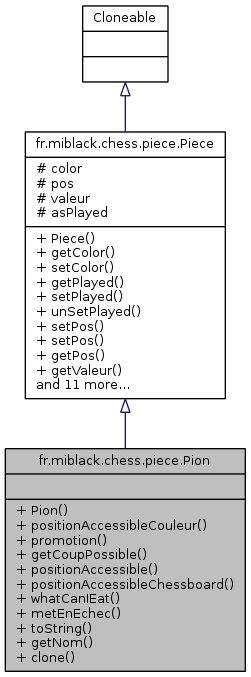
\includegraphics[height=550pt]{classfr_1_1miblack_1_1chess_1_1piece_1_1Pion__inherit__graph}
\end{center}
\end{figure}


Collaboration diagram for fr.\-miblack.\-chess.\-piece.\-Pion\-:
\nopagebreak
\begin{figure}[H]
\begin{center}
\leavevmode
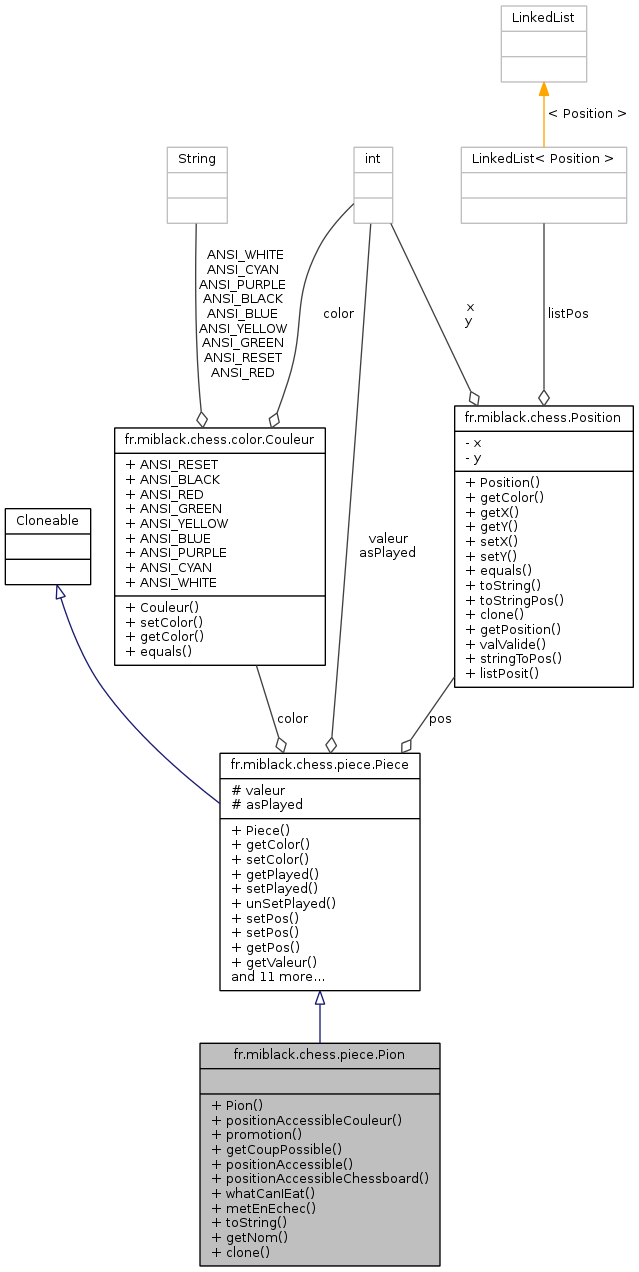
\includegraphics[height=550pt]{classfr_1_1miblack_1_1chess_1_1piece_1_1Pion__coll__graph}
\end{center}
\end{figure}
\subsection*{Public Member Functions}
\begin{DoxyCompactItemize}
\item 
{\bf Pion} ({\bf Couleur} {\bf color}, {\bf Position} {\bf pos}, int {\bf valeur})
\item 
Linked\-List$<$ {\bf Position} $>$ {\bf position\-Accessible\-Couleur} (int couleur)
\item 
{\bf Piece} {\bf promotion} (String str)
\item 
Linked\-List$<$ {\bf Coup} $>$ {\bf get\-Coup\-Possible} ({\bf Piece} Piece\-Depart, {\bf Partie} ma\-Partie)
\item 
Linked\-List$<$ {\bf Position} $>$ {\bf position\-Accessible} ()
\item 
Linked\-List$<$ {\bf Position} $>$ {\bf position\-Accessible\-Chessboard} ({\bf Echiquier} chess)
\item 
Linked\-List$<$ {\bf Position} $>$ {\bf what\-Can\-I\-Eat} ({\bf Echiquier} chess)
\item 
boolean {\bf met\-En\-Echec} ({\bf Echiquier} chess)
\item 
String {\bf to\-String} ()
\item 
String {\bf get\-Nom} ()
\item 
{\bf Piece} {\bf clone} ()
\end{DoxyCompactItemize}
\subsection*{Additional Inherited Members}


\subsection{Detailed Description}
\begin{DoxyAuthor}{Author}
mi-\/black 
\end{DoxyAuthor}


\subsection{Constructor \& Destructor Documentation}
\index{fr\-::miblack\-::chess\-::piece\-::\-Pion@{fr\-::miblack\-::chess\-::piece\-::\-Pion}!Pion@{Pion}}
\index{Pion@{Pion}!fr::miblack::chess::piece::Pion@{fr\-::miblack\-::chess\-::piece\-::\-Pion}}
\subsubsection[{Pion}]{\setlength{\rightskip}{0pt plus 5cm}fr.\-miblack.\-chess.\-piece.\-Pion.\-Pion (
\begin{DoxyParamCaption}
\item[{{\bf Couleur}}]{color, }
\item[{{\bf Position}}]{pos, }
\item[{int}]{valeur}
\end{DoxyParamCaption}
)}\label{classfr_1_1miblack_1_1chess_1_1piece_1_1Pion_a0980ab8ca4af634d368a66293a413d1b}

\begin{DoxyParams}{Parameters}
{\em color} & \\
\hline
{\em pos} & \\
\hline
{\em valeur} & \\
\hline
\end{DoxyParams}


\subsection{Member Function Documentation}
\index{fr\-::miblack\-::chess\-::piece\-::\-Pion@{fr\-::miblack\-::chess\-::piece\-::\-Pion}!clone@{clone}}
\index{clone@{clone}!fr::miblack::chess::piece::Pion@{fr\-::miblack\-::chess\-::piece\-::\-Pion}}
\subsubsection[{clone}]{\setlength{\rightskip}{0pt plus 5cm}{\bf Piece} fr.\-miblack.\-chess.\-piece.\-Pion.\-clone (
\begin{DoxyParamCaption}
{}
\end{DoxyParamCaption}
)}\label{classfr_1_1miblack_1_1chess_1_1piece_1_1Pion_aca889774de79f97edff2d4d21bfcf77f}
\begin{DoxyReturn}{Returns}

\end{DoxyReturn}
\index{fr\-::miblack\-::chess\-::piece\-::\-Pion@{fr\-::miblack\-::chess\-::piece\-::\-Pion}!get\-Coup\-Possible@{get\-Coup\-Possible}}
\index{get\-Coup\-Possible@{get\-Coup\-Possible}!fr::miblack::chess::piece::Pion@{fr\-::miblack\-::chess\-::piece\-::\-Pion}}
\subsubsection[{get\-Coup\-Possible}]{\setlength{\rightskip}{0pt plus 5cm}Linked\-List$<${\bf Coup}$>$ fr.\-miblack.\-chess.\-piece.\-Pion.\-get\-Coup\-Possible (
\begin{DoxyParamCaption}
\item[{{\bf Piece}}]{Piece\-Depart, }
\item[{{\bf Partie}}]{ma\-Partie}
\end{DoxyParamCaption}
)}\label{classfr_1_1miblack_1_1chess_1_1piece_1_1Pion_a0480e38f7b6f027b01da4bef00f6f3f2}

\begin{DoxyParams}{Parameters}
{\em Piece\-Depart} & \\
\hline
{\em ma\-Partie} & \\
\hline
\end{DoxyParams}
\begin{DoxyReturn}{Returns}

\end{DoxyReturn}


Reimplemented from {\bf fr.\-miblack.\-chess.\-piece.\-Piece} \doxyref{}{p.}{classfr_1_1miblack_1_1chess_1_1piece_1_1Piece_ace5ed8c4d7f922076255d5aa0733e51e}.

\index{fr\-::miblack\-::chess\-::piece\-::\-Pion@{fr\-::miblack\-::chess\-::piece\-::\-Pion}!get\-Nom@{get\-Nom}}
\index{get\-Nom@{get\-Nom}!fr::miblack::chess::piece::Pion@{fr\-::miblack\-::chess\-::piece\-::\-Pion}}
\subsubsection[{get\-Nom}]{\setlength{\rightskip}{0pt plus 5cm}String fr.\-miblack.\-chess.\-piece.\-Pion.\-get\-Nom (
\begin{DoxyParamCaption}
{}
\end{DoxyParamCaption}
)}\label{classfr_1_1miblack_1_1chess_1_1piece_1_1Pion_a6a0712e0005efb52ae3ccf7b96be4957}
\begin{DoxyReturn}{Returns}

\end{DoxyReturn}


Reimplemented from {\bf fr.\-miblack.\-chess.\-piece.\-Piece} \doxyref{}{p.}{classfr_1_1miblack_1_1chess_1_1piece_1_1Piece_a68bb44429e21b7f64511a91a0861dde4}.

\index{fr\-::miblack\-::chess\-::piece\-::\-Pion@{fr\-::miblack\-::chess\-::piece\-::\-Pion}!met\-En\-Echec@{met\-En\-Echec}}
\index{met\-En\-Echec@{met\-En\-Echec}!fr::miblack::chess::piece::Pion@{fr\-::miblack\-::chess\-::piece\-::\-Pion}}
\subsubsection[{met\-En\-Echec}]{\setlength{\rightskip}{0pt plus 5cm}boolean fr.\-miblack.\-chess.\-piece.\-Pion.\-met\-En\-Echec (
\begin{DoxyParamCaption}
\item[{{\bf Echiquier}}]{chess}
\end{DoxyParamCaption}
)}\label{classfr_1_1miblack_1_1chess_1_1piece_1_1Pion_a1f472efbefe3f2914bc24a934e774b31}

\begin{DoxyParams}{Parameters}
{\em chess} & \\
\hline
\end{DoxyParams}
\begin{DoxyReturn}{Returns}

\end{DoxyReturn}
\index{fr\-::miblack\-::chess\-::piece\-::\-Pion@{fr\-::miblack\-::chess\-::piece\-::\-Pion}!position\-Accessible@{position\-Accessible}}
\index{position\-Accessible@{position\-Accessible}!fr::miblack::chess::piece::Pion@{fr\-::miblack\-::chess\-::piece\-::\-Pion}}
\subsubsection[{position\-Accessible}]{\setlength{\rightskip}{0pt plus 5cm}Linked\-List$<${\bf Position}$>$ fr.\-miblack.\-chess.\-piece.\-Pion.\-position\-Accessible (
\begin{DoxyParamCaption}
{}
\end{DoxyParamCaption}
)\hspace{0.3cm}{\ttfamily [virtual]}}\label{classfr_1_1miblack_1_1chess_1_1piece_1_1Pion_ad781b079c949af93e742badb99a47608}
\begin{DoxyReturn}{Returns}
List of position where one piece can be going 
\end{DoxyReturn}


Implements {\bf fr.\-miblack.\-chess.\-piece.\-Piece} \doxyref{}{p.}{classfr_1_1miblack_1_1chess_1_1piece_1_1Piece_ad5cdbd635ec706f16d57dccf1b8c456e}.

\index{fr\-::miblack\-::chess\-::piece\-::\-Pion@{fr\-::miblack\-::chess\-::piece\-::\-Pion}!position\-Accessible\-Chessboard@{position\-Accessible\-Chessboard}}
\index{position\-Accessible\-Chessboard@{position\-Accessible\-Chessboard}!fr::miblack::chess::piece::Pion@{fr\-::miblack\-::chess\-::piece\-::\-Pion}}
\subsubsection[{position\-Accessible\-Chessboard}]{\setlength{\rightskip}{0pt plus 5cm}Linked\-List$<${\bf Position}$>$ fr.\-miblack.\-chess.\-piece.\-Pion.\-position\-Accessible\-Chessboard (
\begin{DoxyParamCaption}
\item[{{\bf Echiquier}}]{chess}
\end{DoxyParamCaption}
)\hspace{0.3cm}{\ttfamily [virtual]}}\label{classfr_1_1miblack_1_1chess_1_1piece_1_1Pion_afd1ccbe76aef6117fd63b985913c3a10}
\begin{DoxyReturn}{Returns}
List of position where one piece can be going with restriction of the chessboard 
\end{DoxyReturn}


Implements {\bf fr.\-miblack.\-chess.\-piece.\-Piece} \doxyref{}{p.}{classfr_1_1miblack_1_1chess_1_1piece_1_1Piece_ac1222bad9bf13533eecec2b8d99e24c6}.

\index{fr\-::miblack\-::chess\-::piece\-::\-Pion@{fr\-::miblack\-::chess\-::piece\-::\-Pion}!position\-Accessible\-Couleur@{position\-Accessible\-Couleur}}
\index{position\-Accessible\-Couleur@{position\-Accessible\-Couleur}!fr::miblack::chess::piece::Pion@{fr\-::miblack\-::chess\-::piece\-::\-Pion}}
\subsubsection[{position\-Accessible\-Couleur}]{\setlength{\rightskip}{0pt plus 5cm}Linked\-List$<${\bf Position}$>$ fr.\-miblack.\-chess.\-piece.\-Pion.\-position\-Accessible\-Couleur (
\begin{DoxyParamCaption}
\item[{int}]{couleur}
\end{DoxyParamCaption}
)}\label{classfr_1_1miblack_1_1chess_1_1piece_1_1Pion_a4a6114767d591a34ca479a24a14f6b8b}

\begin{DoxyParams}{Parameters}
{\em couleur} & \\
\hline
\end{DoxyParams}
\begin{DoxyReturn}{Returns}

\end{DoxyReturn}
\index{fr\-::miblack\-::chess\-::piece\-::\-Pion@{fr\-::miblack\-::chess\-::piece\-::\-Pion}!promotion@{promotion}}
\index{promotion@{promotion}!fr::miblack::chess::piece::Pion@{fr\-::miblack\-::chess\-::piece\-::\-Pion}}
\subsubsection[{promotion}]{\setlength{\rightskip}{0pt plus 5cm}{\bf Piece} fr.\-miblack.\-chess.\-piece.\-Pion.\-promotion (
\begin{DoxyParamCaption}
\item[{String}]{str}
\end{DoxyParamCaption}
)}\label{classfr_1_1miblack_1_1chess_1_1piece_1_1Pion_a4569bca3d9eeee097750d26270b12483}

\begin{DoxyParams}{Parameters}
{\em str} & chaine de promotion \\
\hline
\end{DoxyParams}
\begin{DoxyReturn}{Returns}

\end{DoxyReturn}
\index{fr\-::miblack\-::chess\-::piece\-::\-Pion@{fr\-::miblack\-::chess\-::piece\-::\-Pion}!to\-String@{to\-String}}
\index{to\-String@{to\-String}!fr::miblack::chess::piece::Pion@{fr\-::miblack\-::chess\-::piece\-::\-Pion}}
\subsubsection[{to\-String}]{\setlength{\rightskip}{0pt plus 5cm}String fr.\-miblack.\-chess.\-piece.\-Pion.\-to\-String (
\begin{DoxyParamCaption}
{}
\end{DoxyParamCaption}
)}\label{classfr_1_1miblack_1_1chess_1_1piece_1_1Pion_abd08277b50a30a03e1dd50be63939b52}
\begin{DoxyReturn}{Returns}

\end{DoxyReturn}
\index{fr\-::miblack\-::chess\-::piece\-::\-Pion@{fr\-::miblack\-::chess\-::piece\-::\-Pion}!what\-Can\-I\-Eat@{what\-Can\-I\-Eat}}
\index{what\-Can\-I\-Eat@{what\-Can\-I\-Eat}!fr::miblack::chess::piece::Pion@{fr\-::miblack\-::chess\-::piece\-::\-Pion}}
\subsubsection[{what\-Can\-I\-Eat}]{\setlength{\rightskip}{0pt plus 5cm}Linked\-List$<${\bf Position}$>$ fr.\-miblack.\-chess.\-piece.\-Pion.\-what\-Can\-I\-Eat (
\begin{DoxyParamCaption}
\item[{{\bf Echiquier}}]{chess}
\end{DoxyParamCaption}
)\hspace{0.3cm}{\ttfamily [virtual]}}\label{classfr_1_1miblack_1_1chess_1_1piece_1_1Pion_af7b15f6d766ddc6ad0fec0af8041780a}

\begin{DoxyParams}{Parameters}
{\em chess} & l'echiquier \\
\hline
\end{DoxyParams}
\begin{DoxyReturn}{Returns}
Liste des position capturables 
\end{DoxyReturn}


Implements {\bf fr.\-miblack.\-chess.\-piece.\-Piece} \doxyref{}{p.}{classfr_1_1miblack_1_1chess_1_1piece_1_1Piece_af18b3bc007e0e50740de39142a5b2919}.



The documentation for this class was generated from the following file\-:\begin{DoxyCompactItemize}
\item 
fr/miblack/chess/piece/{\bf Pion.\-java}\end{DoxyCompactItemize}

\section{fr.\-miblack.\-chess.\-Position Class Reference}
\label{classfr_1_1miblack_1_1chess_1_1Position}\index{fr.\-miblack.\-chess.\-Position@{fr.\-miblack.\-chess.\-Position}}


Collaboration diagram for fr.\-miblack.\-chess.\-Position\-:
\nopagebreak
\begin{figure}[H]
\begin{center}
\leavevmode
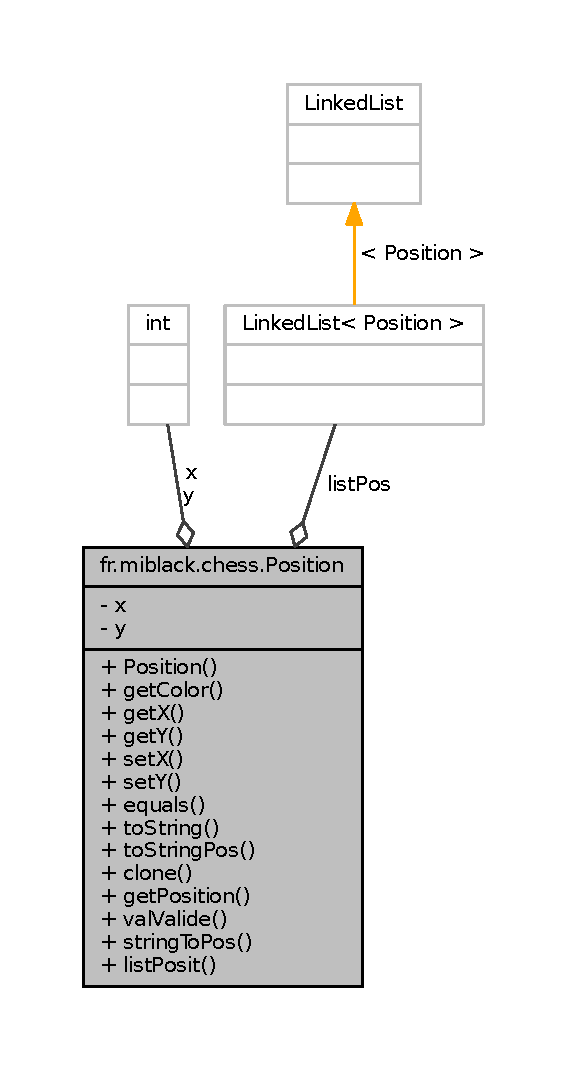
\includegraphics[width=274pt]{classfr_1_1miblack_1_1chess_1_1Position__coll__graph}
\end{center}
\end{figure}
\subsection*{Public Member Functions}
\begin{DoxyCompactItemize}
\item 
{\bf Position} (int {\bf x}, int {\bf y})
\item 
int {\bf get\-Color} ()
\item 
int {\bf get\-X} ()
\item 
int {\bf get\-Y} ()
\item 
void {\bf set\-X} (int {\bf x})
\item 
void {\bf set\-Y} (int {\bf y})
\item 
boolean {\bf equals} ({\bf Position} pos)
\item 
String {\bf to\-String} ()
\item 
String {\bf to\-String\-Pos} ()
\item 
{\bf Position} {\bf clone} ()
\end{DoxyCompactItemize}
\subsection*{Static Public Member Functions}
\begin{DoxyCompactItemize}
\item 
static {\bf Position} {\bf get\-Position} (int {\bf x}, int {\bf y})
\item 
static boolean {\bf val\-Valide} (int a)
\item 
static {\bf Position} {\bf string\-To\-Pos} (String pos)
\item 
static Linked\-List$<$ {\bf Position} $>$ {\bf list\-Posit} ()
\end{DoxyCompactItemize}
\subsection*{Private Attributes}
\begin{DoxyCompactItemize}
\item 
int {\bf x}
\item 
int {\bf y}
\end{DoxyCompactItemize}
\subsection*{Static Private Attributes}
\begin{DoxyCompactItemize}
\item 
static Linked\-List$<$ {\bf Position} $>$ {\bf list\-Pos} = new Linked\-List$<${\bf Position}$>$()
\end{DoxyCompactItemize}


\subsection{Detailed Description}
Une position est consitué d'un x et d'un y \begin{DoxyAuthor}{Author}
mi-\/black 
\end{DoxyAuthor}


\subsection{Constructor \& Destructor Documentation}
\index{fr\-::miblack\-::chess\-::\-Position@{fr\-::miblack\-::chess\-::\-Position}!Position@{Position}}
\index{Position@{Position}!fr::miblack::chess::Position@{fr\-::miblack\-::chess\-::\-Position}}
\subsubsection[{Position}]{\setlength{\rightskip}{0pt plus 5cm}fr.\-miblack.\-chess.\-Position.\-Position (
\begin{DoxyParamCaption}
\item[{int}]{x, }
\item[{int}]{y}
\end{DoxyParamCaption}
)}\label{classfr_1_1miblack_1_1chess_1_1Position_a6514886f36a1df66a40e32206b9f79c3}

\begin{DoxyParams}{Parameters}
{\em x} & \\
\hline
{\em y} & \\
\hline
\end{DoxyParams}


\subsection{Member Function Documentation}
\index{fr\-::miblack\-::chess\-::\-Position@{fr\-::miblack\-::chess\-::\-Position}!clone@{clone}}
\index{clone@{clone}!fr::miblack::chess::Position@{fr\-::miblack\-::chess\-::\-Position}}
\subsubsection[{clone}]{\setlength{\rightskip}{0pt plus 5cm}{\bf Position} fr.\-miblack.\-chess.\-Position.\-clone (
\begin{DoxyParamCaption}
{}
\end{DoxyParamCaption}
)}\label{classfr_1_1miblack_1_1chess_1_1Position_a902970b0770548326225ff2fa4cc38ff}
\begin{DoxyReturn}{Returns}

\end{DoxyReturn}
\index{fr\-::miblack\-::chess\-::\-Position@{fr\-::miblack\-::chess\-::\-Position}!equals@{equals}}
\index{equals@{equals}!fr::miblack::chess::Position@{fr\-::miblack\-::chess\-::\-Position}}
\subsubsection[{equals}]{\setlength{\rightskip}{0pt plus 5cm}boolean fr.\-miblack.\-chess.\-Position.\-equals (
\begin{DoxyParamCaption}
\item[{{\bf Position}}]{pos}
\end{DoxyParamCaption}
)}\label{classfr_1_1miblack_1_1chess_1_1Position_a7094a3453cb88d76d010800c74abf8b8}

\begin{DoxyParams}{Parameters}
{\em pos} & \\
\hline
\end{DoxyParams}
\begin{DoxyReturn}{Returns}

\end{DoxyReturn}
\index{fr\-::miblack\-::chess\-::\-Position@{fr\-::miblack\-::chess\-::\-Position}!get\-Color@{get\-Color}}
\index{get\-Color@{get\-Color}!fr::miblack::chess::Position@{fr\-::miblack\-::chess\-::\-Position}}
\subsubsection[{get\-Color}]{\setlength{\rightskip}{0pt plus 5cm}int fr.\-miblack.\-chess.\-Position.\-get\-Color (
\begin{DoxyParamCaption}
{}
\end{DoxyParamCaption}
)}\label{classfr_1_1miblack_1_1chess_1_1Position_afdc733da38581f0def274843362b8775}
\begin{DoxyReturn}{Returns}
la couleur d'une position (0 ou 1) 
\end{DoxyReturn}
\index{fr\-::miblack\-::chess\-::\-Position@{fr\-::miblack\-::chess\-::\-Position}!get\-Position@{get\-Position}}
\index{get\-Position@{get\-Position}!fr::miblack::chess::Position@{fr\-::miblack\-::chess\-::\-Position}}
\subsubsection[{get\-Position}]{\setlength{\rightskip}{0pt plus 5cm}static {\bf Position} fr.\-miblack.\-chess.\-Position.\-get\-Position (
\begin{DoxyParamCaption}
\item[{int}]{x, }
\item[{int}]{y}
\end{DoxyParamCaption}
)\hspace{0.3cm}{\ttfamily [static]}}\label{classfr_1_1miblack_1_1chess_1_1Position_a10c462c32e918cfdd8a4f3daaa48f53c}
Fly weight 
\begin{DoxyParams}{Parameters}
{\em x} & \\
\hline
{\em y} & \\
\hline
\end{DoxyParams}
\begin{DoxyReturn}{Returns}
new Pos O\-U pos déjà existante 
\end{DoxyReturn}
\index{fr\-::miblack\-::chess\-::\-Position@{fr\-::miblack\-::chess\-::\-Position}!get\-X@{get\-X}}
\index{get\-X@{get\-X}!fr::miblack::chess::Position@{fr\-::miblack\-::chess\-::\-Position}}
\subsubsection[{get\-X}]{\setlength{\rightskip}{0pt plus 5cm}int fr.\-miblack.\-chess.\-Position.\-get\-X (
\begin{DoxyParamCaption}
{}
\end{DoxyParamCaption}
)}\label{classfr_1_1miblack_1_1chess_1_1Position_af16ee79dc63b76cd2260e5c42a4db8c1}
\begin{DoxyReturn}{Returns}

\end{DoxyReturn}
\index{fr\-::miblack\-::chess\-::\-Position@{fr\-::miblack\-::chess\-::\-Position}!get\-Y@{get\-Y}}
\index{get\-Y@{get\-Y}!fr::miblack::chess::Position@{fr\-::miblack\-::chess\-::\-Position}}
\subsubsection[{get\-Y}]{\setlength{\rightskip}{0pt plus 5cm}int fr.\-miblack.\-chess.\-Position.\-get\-Y (
\begin{DoxyParamCaption}
{}
\end{DoxyParamCaption}
)}\label{classfr_1_1miblack_1_1chess_1_1Position_a5b6fe6685e7ee195bb072f418cfc5cc9}
\begin{DoxyReturn}{Returns}

\end{DoxyReturn}
\index{fr\-::miblack\-::chess\-::\-Position@{fr\-::miblack\-::chess\-::\-Position}!list\-Posit@{list\-Posit}}
\index{list\-Posit@{list\-Posit}!fr::miblack::chess::Position@{fr\-::miblack\-::chess\-::\-Position}}
\subsubsection[{list\-Posit}]{\setlength{\rightskip}{0pt plus 5cm}static Linked\-List$<${\bf Position}$>$ fr.\-miblack.\-chess.\-Position.\-list\-Posit (
\begin{DoxyParamCaption}
{}
\end{DoxyParamCaption}
)\hspace{0.3cm}{\ttfamily [static]}}\label{classfr_1_1miblack_1_1chess_1_1Position_a966c06c686030c93205e9d1da686903c}
\begin{DoxyReturn}{Returns}
la liste des positions 
\end{DoxyReturn}
\index{fr\-::miblack\-::chess\-::\-Position@{fr\-::miblack\-::chess\-::\-Position}!set\-X@{set\-X}}
\index{set\-X@{set\-X}!fr::miblack::chess::Position@{fr\-::miblack\-::chess\-::\-Position}}
\subsubsection[{set\-X}]{\setlength{\rightskip}{0pt plus 5cm}void fr.\-miblack.\-chess.\-Position.\-set\-X (
\begin{DoxyParamCaption}
\item[{int}]{x}
\end{DoxyParamCaption}
)}\label{classfr_1_1miblack_1_1chess_1_1Position_a1d05bbfd5db8b338545ead0a6a9b49a7}

\begin{DoxyParams}{Parameters}
{\em x} & \\
\hline
\end{DoxyParams}
\index{fr\-::miblack\-::chess\-::\-Position@{fr\-::miblack\-::chess\-::\-Position}!set\-Y@{set\-Y}}
\index{set\-Y@{set\-Y}!fr::miblack::chess::Position@{fr\-::miblack\-::chess\-::\-Position}}
\subsubsection[{set\-Y}]{\setlength{\rightskip}{0pt plus 5cm}void fr.\-miblack.\-chess.\-Position.\-set\-Y (
\begin{DoxyParamCaption}
\item[{int}]{y}
\end{DoxyParamCaption}
)}\label{classfr_1_1miblack_1_1chess_1_1Position_a5329284c5a0421535f2bf04244a48048}

\begin{DoxyParams}{Parameters}
{\em y} & \\
\hline
\end{DoxyParams}
\index{fr\-::miblack\-::chess\-::\-Position@{fr\-::miblack\-::chess\-::\-Position}!string\-To\-Pos@{string\-To\-Pos}}
\index{string\-To\-Pos@{string\-To\-Pos}!fr::miblack::chess::Position@{fr\-::miblack\-::chess\-::\-Position}}
\subsubsection[{string\-To\-Pos}]{\setlength{\rightskip}{0pt plus 5cm}static {\bf Position} fr.\-miblack.\-chess.\-Position.\-string\-To\-Pos (
\begin{DoxyParamCaption}
\item[{String}]{pos}
\end{DoxyParamCaption}
)\hspace{0.3cm}{\ttfamily [static]}}\label{classfr_1_1miblack_1_1chess_1_1Position_a1b5984f9a313ac741ff740b432196f47}

\begin{DoxyParams}{Parameters}
{\em pos} & \\
\hline
\end{DoxyParams}
\begin{DoxyReturn}{Returns}
la position equivalante a la chaine passee 
\end{DoxyReturn}
\index{fr\-::miblack\-::chess\-::\-Position@{fr\-::miblack\-::chess\-::\-Position}!to\-String@{to\-String}}
\index{to\-String@{to\-String}!fr::miblack::chess::Position@{fr\-::miblack\-::chess\-::\-Position}}
\subsubsection[{to\-String}]{\setlength{\rightskip}{0pt plus 5cm}String fr.\-miblack.\-chess.\-Position.\-to\-String (
\begin{DoxyParamCaption}
{}
\end{DoxyParamCaption}
)}\label{classfr_1_1miblack_1_1chess_1_1Position_a0610d0d0830d94a03887303c9edef19d}
\begin{DoxyReturn}{Returns}

\end{DoxyReturn}
\index{fr\-::miblack\-::chess\-::\-Position@{fr\-::miblack\-::chess\-::\-Position}!to\-String\-Pos@{to\-String\-Pos}}
\index{to\-String\-Pos@{to\-String\-Pos}!fr::miblack::chess::Position@{fr\-::miblack\-::chess\-::\-Position}}
\subsubsection[{to\-String\-Pos}]{\setlength{\rightskip}{0pt plus 5cm}String fr.\-miblack.\-chess.\-Position.\-to\-String\-Pos (
\begin{DoxyParamCaption}
{}
\end{DoxyParamCaption}
)}\label{classfr_1_1miblack_1_1chess_1_1Position_a1ed78d1d48c962a5261257e4c49cfe3a}
\begin{DoxyReturn}{Returns}
chaine , 00 =$>$ a1 
\end{DoxyReturn}
\index{fr\-::miblack\-::chess\-::\-Position@{fr\-::miblack\-::chess\-::\-Position}!val\-Valide@{val\-Valide}}
\index{val\-Valide@{val\-Valide}!fr::miblack::chess::Position@{fr\-::miblack\-::chess\-::\-Position}}
\subsubsection[{val\-Valide}]{\setlength{\rightskip}{0pt plus 5cm}static boolean fr.\-miblack.\-chess.\-Position.\-val\-Valide (
\begin{DoxyParamCaption}
\item[{int}]{a}
\end{DoxyParamCaption}
)\hspace{0.3cm}{\ttfamily [static]}}\label{classfr_1_1miblack_1_1chess_1_1Position_a81852eae590f3d87038794b53e88e59d}

\begin{DoxyParams}{Parameters}
{\em a} & \\
\hline
\end{DoxyParams}
\begin{DoxyReturn}{Returns}
a$>$=0 \&\& a$<$8 
\end{DoxyReturn}


\subsection{Member Data Documentation}
\index{fr\-::miblack\-::chess\-::\-Position@{fr\-::miblack\-::chess\-::\-Position}!list\-Pos@{list\-Pos}}
\index{list\-Pos@{list\-Pos}!fr::miblack::chess::Position@{fr\-::miblack\-::chess\-::\-Position}}
\subsubsection[{list\-Pos}]{\setlength{\rightskip}{0pt plus 5cm}Linked\-List$<${\bf Position}$>$ fr.\-miblack.\-chess.\-Position.\-list\-Pos = new Linked\-List$<${\bf Position}$>$()\hspace{0.3cm}{\ttfamily [static]}, {\ttfamily [private]}}\label{classfr_1_1miblack_1_1chess_1_1Position_a2969a21255714dbb7ebcacb104b4a86c}
\index{fr\-::miblack\-::chess\-::\-Position@{fr\-::miblack\-::chess\-::\-Position}!x@{x}}
\index{x@{x}!fr::miblack::chess::Position@{fr\-::miblack\-::chess\-::\-Position}}
\subsubsection[{x}]{\setlength{\rightskip}{0pt plus 5cm}int fr.\-miblack.\-chess.\-Position.\-x\hspace{0.3cm}{\ttfamily [private]}}\label{classfr_1_1miblack_1_1chess_1_1Position_a1479cde5381c4b42e7efeeff29d33645}
\index{fr\-::miblack\-::chess\-::\-Position@{fr\-::miblack\-::chess\-::\-Position}!y@{y}}
\index{y@{y}!fr::miblack::chess::Position@{fr\-::miblack\-::chess\-::\-Position}}
\subsubsection[{y}]{\setlength{\rightskip}{0pt plus 5cm}int fr.\-miblack.\-chess.\-Position.\-y\hspace{0.3cm}{\ttfamily [private]}}\label{classfr_1_1miblack_1_1chess_1_1Position_a58e2521bb0bd5fb9163418ce7b0e400f}


The documentation for this class was generated from the following file\-:\begin{DoxyCompactItemize}
\item 
fr/miblack/chess/{\bf Position.\-java}\end{DoxyCompactItemize}

\section{fr.\-miblack.\-chess.\-piece.\-Roi Class Reference}
\label{classfr_1_1miblack_1_1chess_1_1piece_1_1Roi}\index{fr.\-miblack.\-chess.\-piece.\-Roi@{fr.\-miblack.\-chess.\-piece.\-Roi}}
Inheritance diagram for fr.\-miblack.\-chess.\-piece.\-Roi\-:\begin{figure}[H]
\begin{center}
\leavevmode
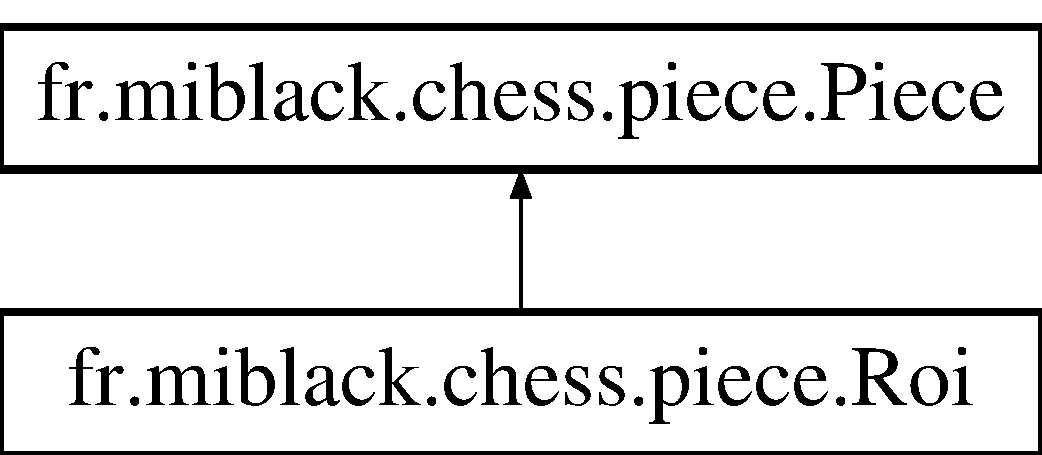
\includegraphics[height=2.000000cm]{classfr_1_1miblack_1_1chess_1_1piece_1_1Roi}
\end{center}
\end{figure}
\subsection*{Public Member Functions}
\begin{DoxyCompactItemize}
\item 
{\bf Roi} ({\bf Couleur} {\bf color}, {\bf Position} {\bf pos}, int {\bf valeur})
\item 
Linked\-List$<$ {\bf Position} $>$ {\bf position\-Accessible} ()
\item 
Linked\-List$<$ {\bf Position} $>$ {\bf position\-Accessible\-Chessboard} ({\bf Echiquier} chess)
\item 
Linked\-List$<$ {\bf Position} $>$ {\bf what\-Can\-I\-Eat} ({\bf Echiquier} chess)
\item 
String {\bf to\-String} ()
\item 
String {\bf get\-Nom} ()
\item 
{\bf Piece} {\bf clone} ()
\end{DoxyCompactItemize}
\subsection*{Additional Inherited Members}


\subsection{Detailed Description}
\begin{DoxyAuthor}{Author}
mi-\/black 
\end{DoxyAuthor}


\subsection{Constructor \& Destructor Documentation}
\index{fr\-::miblack\-::chess\-::piece\-::\-Roi@{fr\-::miblack\-::chess\-::piece\-::\-Roi}!Roi@{Roi}}
\index{Roi@{Roi}!fr::miblack::chess::piece::Roi@{fr\-::miblack\-::chess\-::piece\-::\-Roi}}
\subsubsection[{Roi}]{\setlength{\rightskip}{0pt plus 5cm}fr.\-miblack.\-chess.\-piece.\-Roi.\-Roi (
\begin{DoxyParamCaption}
\item[{{\bf Couleur}}]{color, }
\item[{{\bf Position}}]{pos, }
\item[{int}]{valeur}
\end{DoxyParamCaption}
)}\label{classfr_1_1miblack_1_1chess_1_1piece_1_1Roi_a64b123f677774360e99519d43de3caac}

\begin{DoxyParams}{Parameters}
{\em color} & \\
\hline
{\em pos} & \\
\hline
{\em valeur} & \\
\hline
\end{DoxyParams}


\subsection{Member Function Documentation}
\index{fr\-::miblack\-::chess\-::piece\-::\-Roi@{fr\-::miblack\-::chess\-::piece\-::\-Roi}!clone@{clone}}
\index{clone@{clone}!fr::miblack::chess::piece::Roi@{fr\-::miblack\-::chess\-::piece\-::\-Roi}}
\subsubsection[{clone}]{\setlength{\rightskip}{0pt plus 5cm}{\bf Piece} fr.\-miblack.\-chess.\-piece.\-Roi.\-clone (
\begin{DoxyParamCaption}
{}
\end{DoxyParamCaption}
)}\label{classfr_1_1miblack_1_1chess_1_1piece_1_1Roi_a8ece0d5da9fc3c983d6ca453c2ecf56f}
\begin{DoxyReturn}{Returns}

\end{DoxyReturn}
\index{fr\-::miblack\-::chess\-::piece\-::\-Roi@{fr\-::miblack\-::chess\-::piece\-::\-Roi}!get\-Nom@{get\-Nom}}
\index{get\-Nom@{get\-Nom}!fr::miblack::chess::piece::Roi@{fr\-::miblack\-::chess\-::piece\-::\-Roi}}
\subsubsection[{get\-Nom}]{\setlength{\rightskip}{0pt plus 5cm}String fr.\-miblack.\-chess.\-piece.\-Roi.\-get\-Nom (
\begin{DoxyParamCaption}
{}
\end{DoxyParamCaption}
)}\label{classfr_1_1miblack_1_1chess_1_1piece_1_1Roi_ae42ca462315ecdfd651c66a126cea358}
\begin{DoxyReturn}{Returns}

\end{DoxyReturn}


Reimplemented from {\bf fr.\-miblack.\-chess.\-piece.\-Piece} \doxyref{}{p.}{classfr_1_1miblack_1_1chess_1_1piece_1_1Piece_a68bb44429e21b7f64511a91a0861dde4}.

\index{fr\-::miblack\-::chess\-::piece\-::\-Roi@{fr\-::miblack\-::chess\-::piece\-::\-Roi}!position\-Accessible@{position\-Accessible}}
\index{position\-Accessible@{position\-Accessible}!fr::miblack::chess::piece::Roi@{fr\-::miblack\-::chess\-::piece\-::\-Roi}}
\subsubsection[{position\-Accessible}]{\setlength{\rightskip}{0pt plus 5cm}Linked\-List$<${\bf Position}$>$ fr.\-miblack.\-chess.\-piece.\-Roi.\-position\-Accessible (
\begin{DoxyParamCaption}
{}
\end{DoxyParamCaption}
)\hspace{0.3cm}{\ttfamily [virtual]}}\label{classfr_1_1miblack_1_1chess_1_1piece_1_1Roi_aafff669d094d5adcc5b8e7e79563d6c5}
\begin{DoxyReturn}{Returns}
List of position where one piece can be going 
\end{DoxyReturn}


Implements {\bf fr.\-miblack.\-chess.\-piece.\-Piece} \doxyref{}{p.}{classfr_1_1miblack_1_1chess_1_1piece_1_1Piece_ad5cdbd635ec706f16d57dccf1b8c456e}.

\index{fr\-::miblack\-::chess\-::piece\-::\-Roi@{fr\-::miblack\-::chess\-::piece\-::\-Roi}!position\-Accessible\-Chessboard@{position\-Accessible\-Chessboard}}
\index{position\-Accessible\-Chessboard@{position\-Accessible\-Chessboard}!fr::miblack::chess::piece::Roi@{fr\-::miblack\-::chess\-::piece\-::\-Roi}}
\subsubsection[{position\-Accessible\-Chessboard}]{\setlength{\rightskip}{0pt plus 5cm}Linked\-List$<${\bf Position}$>$ fr.\-miblack.\-chess.\-piece.\-Roi.\-position\-Accessible\-Chessboard (
\begin{DoxyParamCaption}
\item[{{\bf Echiquier}}]{chess}
\end{DoxyParamCaption}
)\hspace{0.3cm}{\ttfamily [virtual]}}\label{classfr_1_1miblack_1_1chess_1_1piece_1_1Roi_ad6fac5991349c7580cee1726d410a149}
\begin{DoxyReturn}{Returns}
List of position where one piece can be going with restriction of the chessboard 
\end{DoxyReturn}


Implements {\bf fr.\-miblack.\-chess.\-piece.\-Piece} \doxyref{}{p.}{classfr_1_1miblack_1_1chess_1_1piece_1_1Piece_ac1222bad9bf13533eecec2b8d99e24c6}.

\index{fr\-::miblack\-::chess\-::piece\-::\-Roi@{fr\-::miblack\-::chess\-::piece\-::\-Roi}!to\-String@{to\-String}}
\index{to\-String@{to\-String}!fr::miblack::chess::piece::Roi@{fr\-::miblack\-::chess\-::piece\-::\-Roi}}
\subsubsection[{to\-String}]{\setlength{\rightskip}{0pt plus 5cm}String fr.\-miblack.\-chess.\-piece.\-Roi.\-to\-String (
\begin{DoxyParamCaption}
{}
\end{DoxyParamCaption}
)}\label{classfr_1_1miblack_1_1chess_1_1piece_1_1Roi_ae2348d613779c2b6a06473e38ab1672c}
\begin{DoxyReturn}{Returns}

\end{DoxyReturn}
\index{fr\-::miblack\-::chess\-::piece\-::\-Roi@{fr\-::miblack\-::chess\-::piece\-::\-Roi}!what\-Can\-I\-Eat@{what\-Can\-I\-Eat}}
\index{what\-Can\-I\-Eat@{what\-Can\-I\-Eat}!fr::miblack::chess::piece::Roi@{fr\-::miblack\-::chess\-::piece\-::\-Roi}}
\subsubsection[{what\-Can\-I\-Eat}]{\setlength{\rightskip}{0pt plus 5cm}Linked\-List$<${\bf Position}$>$ fr.\-miblack.\-chess.\-piece.\-Roi.\-what\-Can\-I\-Eat (
\begin{DoxyParamCaption}
\item[{{\bf Echiquier}}]{chess}
\end{DoxyParamCaption}
)\hspace{0.3cm}{\ttfamily [virtual]}}\label{classfr_1_1miblack_1_1chess_1_1piece_1_1Roi_a2d7147993a2be1f2bd6e53f004593ce1}

\begin{DoxyParams}{Parameters}
{\em chess} & l'echiquier \\
\hline
\end{DoxyParams}
\begin{DoxyReturn}{Returns}
Liste des position capturables 
\end{DoxyReturn}


Implements {\bf fr.\-miblack.\-chess.\-piece.\-Piece} \doxyref{}{p.}{classfr_1_1miblack_1_1chess_1_1piece_1_1Piece_af18b3bc007e0e50740de39142a5b2919}.



The documentation for this class was generated from the following file\-:\begin{DoxyCompactItemize}
\item 
fr/miblack/chess/piece/Roi.\-java\end{DoxyCompactItemize}

\section{fr.\-miblack.\-chess.\-affichage.\-Textuelle Class Reference}
\label{classfr_1_1miblack_1_1chess_1_1affichage_1_1Textuelle}\index{fr.\-miblack.\-chess.\-affichage.\-Textuelle@{fr.\-miblack.\-chess.\-affichage.\-Textuelle}}
Inheritance diagram for fr.\-miblack.\-chess.\-affichage.\-Textuelle\-:\begin{figure}[H]
\begin{center}
\leavevmode
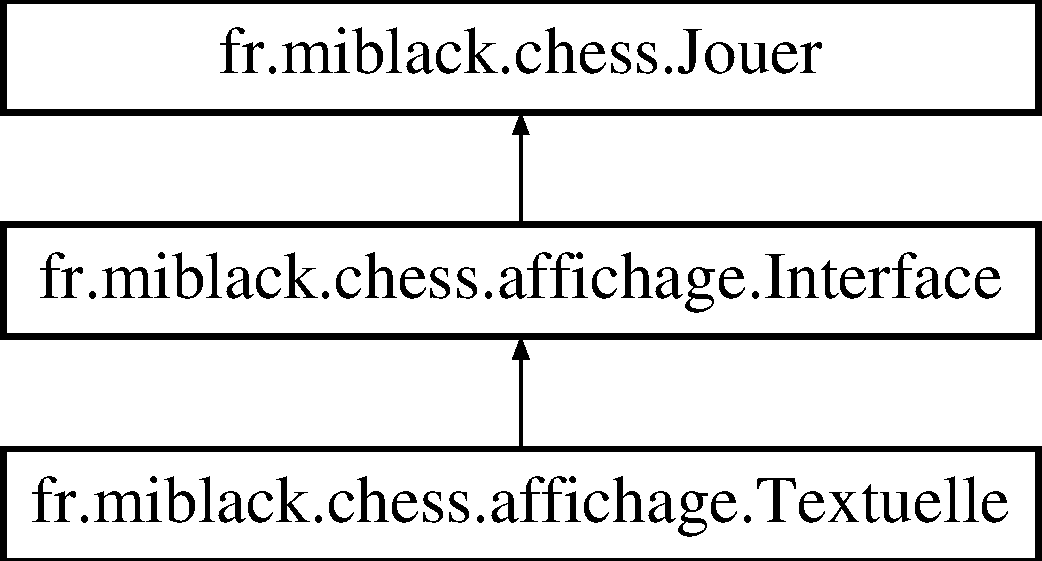
\includegraphics[height=3.000000cm]{classfr_1_1miblack_1_1chess_1_1affichage_1_1Textuelle}
\end{center}
\end{figure}
\subsection*{Public Member Functions}
\begin{DoxyCompactItemize}
\item 
{\bf Textuelle} (String p1, String p2)
\item 
void {\bf jouer\-Partie} ()
\item 
void {\bf proposer\-Save} ({\bf Partie} {\bf ma\-Partie})
\item 
void {\bf afficher\-Echiquier} ()
\item 
{\bf Coup} {\bf jouer\-Coup} ({\bf Partie} g)
\item 
{\bf Coup} {\bf saisir\-Coup} ({\bf Joueur\-Abstract} p, {\bf Echiquier} chess)
\end{DoxyCompactItemize}
\subsection*{Additional Inherited Members}


\subsection{Detailed Description}
\begin{DoxyAuthor}{Author}
mi-\/black 
\end{DoxyAuthor}


\subsection{Constructor \& Destructor Documentation}
\index{fr\-::miblack\-::chess\-::affichage\-::\-Textuelle@{fr\-::miblack\-::chess\-::affichage\-::\-Textuelle}!Textuelle@{Textuelle}}
\index{Textuelle@{Textuelle}!fr::miblack::chess::affichage::Textuelle@{fr\-::miblack\-::chess\-::affichage\-::\-Textuelle}}
\subsubsection[{Textuelle}]{\setlength{\rightskip}{0pt plus 5cm}fr.\-miblack.\-chess.\-affichage.\-Textuelle.\-Textuelle (
\begin{DoxyParamCaption}
\item[{String}]{p1, }
\item[{String}]{p2}
\end{DoxyParamCaption}
)}\label{classfr_1_1miblack_1_1chess_1_1affichage_1_1Textuelle_ac6f276b2f850fe1d26d3cfd24cb18740}

\begin{DoxyParams}{Parameters}
{\em p1} & \\
\hline
{\em p2} & \\
\hline
\end{DoxyParams}


\subsection{Member Function Documentation}
\index{fr\-::miblack\-::chess\-::affichage\-::\-Textuelle@{fr\-::miblack\-::chess\-::affichage\-::\-Textuelle}!afficher\-Echiquier@{afficher\-Echiquier}}
\index{afficher\-Echiquier@{afficher\-Echiquier}!fr::miblack::chess::affichage::Textuelle@{fr\-::miblack\-::chess\-::affichage\-::\-Textuelle}}
\subsubsection[{afficher\-Echiquier}]{\setlength{\rightskip}{0pt plus 5cm}void fr.\-miblack.\-chess.\-affichage.\-Textuelle.\-afficher\-Echiquier (
\begin{DoxyParamCaption}
{}
\end{DoxyParamCaption}
)}\label{classfr_1_1miblack_1_1chess_1_1affichage_1_1Textuelle_a816936b1c3a7b741b86a6dcfc41f4eb7}
\begin{DoxyReturn}{Returns}

\end{DoxyReturn}
\index{fr\-::miblack\-::chess\-::affichage\-::\-Textuelle@{fr\-::miblack\-::chess\-::affichage\-::\-Textuelle}!jouer\-Coup@{jouer\-Coup}}
\index{jouer\-Coup@{jouer\-Coup}!fr::miblack::chess::affichage::Textuelle@{fr\-::miblack\-::chess\-::affichage\-::\-Textuelle}}
\subsubsection[{jouer\-Coup}]{\setlength{\rightskip}{0pt plus 5cm}{\bf Coup} fr.\-miblack.\-chess.\-affichage.\-Textuelle.\-jouer\-Coup (
\begin{DoxyParamCaption}
\item[{{\bf Partie}}]{g}
\end{DoxyParamCaption}
)\hspace{0.3cm}{\ttfamily [virtual]}}\label{classfr_1_1miblack_1_1chess_1_1affichage_1_1Textuelle_a2fe98d89987be73eed0e7d666d16f3f5}

\begin{DoxyParams}{Parameters}
{\em g} & une partie \\
\hline
\end{DoxyParams}
\begin{DoxyReturn}{Returns}
le coup Joué 
\end{DoxyReturn}


Implements {\bf fr.\-miblack.\-chess.\-affichage.\-Interface} \doxyref{}{p.}{classfr_1_1miblack_1_1chess_1_1affichage_1_1Interface_a16a7abd6c521cb1e9cdafb5f586db68b}.

\index{fr\-::miblack\-::chess\-::affichage\-::\-Textuelle@{fr\-::miblack\-::chess\-::affichage\-::\-Textuelle}!jouer\-Partie@{jouer\-Partie}}
\index{jouer\-Partie@{jouer\-Partie}!fr::miblack::chess::affichage::Textuelle@{fr\-::miblack\-::chess\-::affichage\-::\-Textuelle}}
\subsubsection[{jouer\-Partie}]{\setlength{\rightskip}{0pt plus 5cm}void fr.\-miblack.\-chess.\-affichage.\-Textuelle.\-jouer\-Partie (
\begin{DoxyParamCaption}
{}
\end{DoxyParamCaption}
)}\label{classfr_1_1miblack_1_1chess_1_1affichage_1_1Textuelle_ae545b7baa8fee49040a801c308d95cba}
le déroulement de la partie \index{fr\-::miblack\-::chess\-::affichage\-::\-Textuelle@{fr\-::miblack\-::chess\-::affichage\-::\-Textuelle}!proposer\-Save@{proposer\-Save}}
\index{proposer\-Save@{proposer\-Save}!fr::miblack::chess::affichage::Textuelle@{fr\-::miblack\-::chess\-::affichage\-::\-Textuelle}}
\subsubsection[{proposer\-Save}]{\setlength{\rightskip}{0pt plus 5cm}void fr.\-miblack.\-chess.\-affichage.\-Textuelle.\-proposer\-Save (
\begin{DoxyParamCaption}
\item[{{\bf Partie}}]{ma\-Partie}
\end{DoxyParamCaption}
)}\label{classfr_1_1miblack_1_1chess_1_1affichage_1_1Textuelle_afbec58022288822aa79fa83a0b5047bb}
propose si l'on veux une sauvegarde


\begin{DoxyParams}{Parameters}
{\em ma\-Partie} & \\
\hline
\end{DoxyParams}
\index{fr\-::miblack\-::chess\-::affichage\-::\-Textuelle@{fr\-::miblack\-::chess\-::affichage\-::\-Textuelle}!saisir\-Coup@{saisir\-Coup}}
\index{saisir\-Coup@{saisir\-Coup}!fr::miblack::chess::affichage::Textuelle@{fr\-::miblack\-::chess\-::affichage\-::\-Textuelle}}
\subsubsection[{saisir\-Coup}]{\setlength{\rightskip}{0pt plus 5cm}{\bf Coup} fr.\-miblack.\-chess.\-affichage.\-Textuelle.\-saisir\-Coup (
\begin{DoxyParamCaption}
\item[{{\bf Joueur\-Abstract}}]{p, }
\item[{{\bf Echiquier}}]{chess}
\end{DoxyParamCaption}
)}\label{classfr_1_1miblack_1_1chess_1_1affichage_1_1Textuelle_a6f9595319c502b6c1c2ecac48cfae6c3}

\begin{DoxyParams}{Parameters}
{\em p} & le joueur \\
\hline
{\em chess} & l'echiquier \\
\hline
\end{DoxyParams}
\begin{DoxyReturn}{Returns}
le coup saisi en textuelle 
\end{DoxyReturn}


The documentation for this class was generated from the following file\-:\begin{DoxyCompactItemize}
\item 
fr/miblack/chess/affichage/Textuelle.\-java\end{DoxyCompactItemize}

\section{fr.\-miblack.\-chess.\-piece.\-Tour Class Reference}
\label{classfr_1_1miblack_1_1chess_1_1piece_1_1Tour}\index{fr.\-miblack.\-chess.\-piece.\-Tour@{fr.\-miblack.\-chess.\-piece.\-Tour}}
Inheritance diagram for fr.\-miblack.\-chess.\-piece.\-Tour\-:\begin{figure}[H]
\begin{center}
\leavevmode
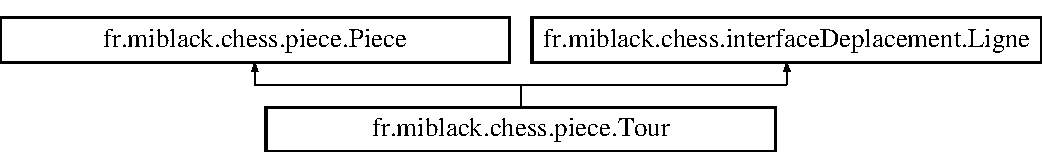
\includegraphics[height=2.000000cm]{classfr_1_1miblack_1_1chess_1_1piece_1_1Tour}
\end{center}
\end{figure}
\subsection*{Public Member Functions}
\begin{DoxyCompactItemize}
\item 
{\bf Tour} ({\bf Couleur} {\bf color}, {\bf Position} {\bf pos}, int {\bf valeur})
\item 
Linked\-List$<$ {\bf Position} $>$ {\bf position\-Accessible} ()
\item 
Linked\-List$<$ {\bf Position} $>$ {\bf position\-Ligne} ()
\item 
Linked\-List$<$ {\bf Position} $>$ {\bf position\-Accessible\-Chessboard} ({\bf Echiquier} chess)
\item 
Linked\-List$<$ {\bf Position} $>$ {\bf position\-Accessible\-Horiz} (int a, {\bf Echiquier} chess)
\item 
Linked\-List$<$ {\bf Position} $>$ {\bf position\-Accessible\-Vert} (int a, {\bf Echiquier} chess)
\item 
Linked\-List$<$ {\bf Position} $>$ {\bf what\-Can\-I\-Eat} ({\bf Echiquier} chess)
\item 
String {\bf to\-String} ()
\item 
String {\bf get\-Nom} ()
\item 
{\bf Piece} {\bf clone} ()
\end{DoxyCompactItemize}
\subsection*{Additional Inherited Members}


\subsection{Detailed Description}
\begin{DoxyAuthor}{Author}
mi-\/black 
\end{DoxyAuthor}


\subsection{Constructor \& Destructor Documentation}
\index{fr\-::miblack\-::chess\-::piece\-::\-Tour@{fr\-::miblack\-::chess\-::piece\-::\-Tour}!Tour@{Tour}}
\index{Tour@{Tour}!fr::miblack::chess::piece::Tour@{fr\-::miblack\-::chess\-::piece\-::\-Tour}}
\subsubsection[{Tour}]{\setlength{\rightskip}{0pt plus 5cm}fr.\-miblack.\-chess.\-piece.\-Tour.\-Tour (
\begin{DoxyParamCaption}
\item[{{\bf Couleur}}]{color, }
\item[{{\bf Position}}]{pos, }
\item[{int}]{valeur}
\end{DoxyParamCaption}
)}\label{classfr_1_1miblack_1_1chess_1_1piece_1_1Tour_a1439bc13af2f5d163906a9a3840d9271}

\begin{DoxyParams}{Parameters}
{\em color} & \\
\hline
{\em pos} & \\
\hline
{\em valeur} & \\
\hline
\end{DoxyParams}


\subsection{Member Function Documentation}
\index{fr\-::miblack\-::chess\-::piece\-::\-Tour@{fr\-::miblack\-::chess\-::piece\-::\-Tour}!clone@{clone}}
\index{clone@{clone}!fr::miblack::chess::piece::Tour@{fr\-::miblack\-::chess\-::piece\-::\-Tour}}
\subsubsection[{clone}]{\setlength{\rightskip}{0pt plus 5cm}{\bf Piece} fr.\-miblack.\-chess.\-piece.\-Tour.\-clone (
\begin{DoxyParamCaption}
{}
\end{DoxyParamCaption}
)}\label{classfr_1_1miblack_1_1chess_1_1piece_1_1Tour_aac45001bfcf6f3ddc1a09b9f0558f205}
\begin{DoxyReturn}{Returns}

\end{DoxyReturn}
\index{fr\-::miblack\-::chess\-::piece\-::\-Tour@{fr\-::miblack\-::chess\-::piece\-::\-Tour}!get\-Nom@{get\-Nom}}
\index{get\-Nom@{get\-Nom}!fr::miblack::chess::piece::Tour@{fr\-::miblack\-::chess\-::piece\-::\-Tour}}
\subsubsection[{get\-Nom}]{\setlength{\rightskip}{0pt plus 5cm}String fr.\-miblack.\-chess.\-piece.\-Tour.\-get\-Nom (
\begin{DoxyParamCaption}
{}
\end{DoxyParamCaption}
)}\label{classfr_1_1miblack_1_1chess_1_1piece_1_1Tour_a80e9e4055be5dadc948b3e8ec9bf22a5}
\begin{DoxyReturn}{Returns}

\end{DoxyReturn}


Reimplemented from {\bf fr.\-miblack.\-chess.\-piece.\-Piece} \doxyref{}{p.}{classfr_1_1miblack_1_1chess_1_1piece_1_1Piece_a68bb44429e21b7f64511a91a0861dde4}.

\index{fr\-::miblack\-::chess\-::piece\-::\-Tour@{fr\-::miblack\-::chess\-::piece\-::\-Tour}!position\-Accessible@{position\-Accessible}}
\index{position\-Accessible@{position\-Accessible}!fr::miblack::chess::piece::Tour@{fr\-::miblack\-::chess\-::piece\-::\-Tour}}
\subsubsection[{position\-Accessible}]{\setlength{\rightskip}{0pt plus 5cm}Linked\-List$<${\bf Position}$>$ fr.\-miblack.\-chess.\-piece.\-Tour.\-position\-Accessible (
\begin{DoxyParamCaption}
{}
\end{DoxyParamCaption}
)\hspace{0.3cm}{\ttfamily [virtual]}}\label{classfr_1_1miblack_1_1chess_1_1piece_1_1Tour_af607119bd40627dd4f05f6996f598094}
\begin{DoxyReturn}{Returns}
List of position where one piece can be going 
\end{DoxyReturn}


Implements {\bf fr.\-miblack.\-chess.\-piece.\-Piece} \doxyref{}{p.}{classfr_1_1miblack_1_1chess_1_1piece_1_1Piece_ad5cdbd635ec706f16d57dccf1b8c456e}.

\index{fr\-::miblack\-::chess\-::piece\-::\-Tour@{fr\-::miblack\-::chess\-::piece\-::\-Tour}!position\-Accessible\-Chessboard@{position\-Accessible\-Chessboard}}
\index{position\-Accessible\-Chessboard@{position\-Accessible\-Chessboard}!fr::miblack::chess::piece::Tour@{fr\-::miblack\-::chess\-::piece\-::\-Tour}}
\subsubsection[{position\-Accessible\-Chessboard}]{\setlength{\rightskip}{0pt plus 5cm}Linked\-List$<${\bf Position}$>$ fr.\-miblack.\-chess.\-piece.\-Tour.\-position\-Accessible\-Chessboard (
\begin{DoxyParamCaption}
\item[{{\bf Echiquier}}]{chess}
\end{DoxyParamCaption}
)\hspace{0.3cm}{\ttfamily [virtual]}}\label{classfr_1_1miblack_1_1chess_1_1piece_1_1Tour_a68469e2ef16437fe17b81a032d21f83d}
\begin{DoxyReturn}{Returns}
List of position where one piece can be going with restriction of the chessboard 
\end{DoxyReturn}


Implements {\bf fr.\-miblack.\-chess.\-piece.\-Piece} \doxyref{}{p.}{classfr_1_1miblack_1_1chess_1_1piece_1_1Piece_ac1222bad9bf13533eecec2b8d99e24c6}.

\index{fr\-::miblack\-::chess\-::piece\-::\-Tour@{fr\-::miblack\-::chess\-::piece\-::\-Tour}!position\-Accessible\-Horiz@{position\-Accessible\-Horiz}}
\index{position\-Accessible\-Horiz@{position\-Accessible\-Horiz}!fr::miblack::chess::piece::Tour@{fr\-::miblack\-::chess\-::piece\-::\-Tour}}
\subsubsection[{position\-Accessible\-Horiz}]{\setlength{\rightskip}{0pt plus 5cm}Linked\-List$<${\bf Position}$>$ fr.\-miblack.\-chess.\-piece.\-Tour.\-position\-Accessible\-Horiz (
\begin{DoxyParamCaption}
\item[{int}]{a, }
\item[{{\bf Echiquier}}]{chess}
\end{DoxyParamCaption}
)}\label{classfr_1_1miblack_1_1chess_1_1piece_1_1Tour_ae23de8d3e16eee47955c7f4562834c11}

\begin{DoxyParams}{Parameters}
{\em a} & avant ou après \\
\hline
{\em chess} & \\
\hline
\end{DoxyParams}
\begin{DoxyReturn}{Returns}

\end{DoxyReturn}
\index{fr\-::miblack\-::chess\-::piece\-::\-Tour@{fr\-::miblack\-::chess\-::piece\-::\-Tour}!position\-Accessible\-Vert@{position\-Accessible\-Vert}}
\index{position\-Accessible\-Vert@{position\-Accessible\-Vert}!fr::miblack::chess::piece::Tour@{fr\-::miblack\-::chess\-::piece\-::\-Tour}}
\subsubsection[{position\-Accessible\-Vert}]{\setlength{\rightskip}{0pt plus 5cm}Linked\-List$<${\bf Position}$>$ fr.\-miblack.\-chess.\-piece.\-Tour.\-position\-Accessible\-Vert (
\begin{DoxyParamCaption}
\item[{int}]{a, }
\item[{{\bf Echiquier}}]{chess}
\end{DoxyParamCaption}
)}\label{classfr_1_1miblack_1_1chess_1_1piece_1_1Tour_af749ab963675afc704f7c0de275d6fb9}

\begin{DoxyParams}{Parameters}
{\em a} & au dessus et en dessous \\
\hline
{\em chess} & \\
\hline
\end{DoxyParams}
\begin{DoxyReturn}{Returns}

\end{DoxyReturn}
\index{fr\-::miblack\-::chess\-::piece\-::\-Tour@{fr\-::miblack\-::chess\-::piece\-::\-Tour}!position\-Ligne@{position\-Ligne}}
\index{position\-Ligne@{position\-Ligne}!fr::miblack::chess::piece::Tour@{fr\-::miblack\-::chess\-::piece\-::\-Tour}}
\subsubsection[{position\-Ligne}]{\setlength{\rightskip}{0pt plus 5cm}Linked\-List$<${\bf Position}$>$ fr.\-miblack.\-chess.\-piece.\-Tour.\-position\-Ligne (
\begin{DoxyParamCaption}
{}
\end{DoxyParamCaption}
)}\label{classfr_1_1miblack_1_1chess_1_1piece_1_1Tour_aef9cf1b642e1d24904f41d037e29f8a1}
\begin{DoxyReturn}{Returns}
liste des pos en ligne 
\end{DoxyReturn}


Implements {\bf fr.\-miblack.\-chess.\-interface\-Deplacement.\-Ligne} \doxyref{}{p.}{interfacefr_1_1miblack_1_1chess_1_1interfaceDeplacement_1_1Ligne_a55b5c0cdf05915b5996754c845591399}.

\index{fr\-::miblack\-::chess\-::piece\-::\-Tour@{fr\-::miblack\-::chess\-::piece\-::\-Tour}!to\-String@{to\-String}}
\index{to\-String@{to\-String}!fr::miblack::chess::piece::Tour@{fr\-::miblack\-::chess\-::piece\-::\-Tour}}
\subsubsection[{to\-String}]{\setlength{\rightskip}{0pt plus 5cm}String fr.\-miblack.\-chess.\-piece.\-Tour.\-to\-String (
\begin{DoxyParamCaption}
{}
\end{DoxyParamCaption}
)}\label{classfr_1_1miblack_1_1chess_1_1piece_1_1Tour_a1e4863648799eec4ae64cb835a0f316a}
\begin{DoxyReturn}{Returns}

\end{DoxyReturn}
\index{fr\-::miblack\-::chess\-::piece\-::\-Tour@{fr\-::miblack\-::chess\-::piece\-::\-Tour}!what\-Can\-I\-Eat@{what\-Can\-I\-Eat}}
\index{what\-Can\-I\-Eat@{what\-Can\-I\-Eat}!fr::miblack::chess::piece::Tour@{fr\-::miblack\-::chess\-::piece\-::\-Tour}}
\subsubsection[{what\-Can\-I\-Eat}]{\setlength{\rightskip}{0pt plus 5cm}Linked\-List$<${\bf Position}$>$ fr.\-miblack.\-chess.\-piece.\-Tour.\-what\-Can\-I\-Eat (
\begin{DoxyParamCaption}
\item[{{\bf Echiquier}}]{chess}
\end{DoxyParamCaption}
)\hspace{0.3cm}{\ttfamily [virtual]}}\label{classfr_1_1miblack_1_1chess_1_1piece_1_1Tour_a348cb7a05f90052d953596f2c3236e06}

\begin{DoxyParams}{Parameters}
{\em chess} & l'echiquier \\
\hline
\end{DoxyParams}
\begin{DoxyReturn}{Returns}
Liste des position capturables 
\end{DoxyReturn}


Implements {\bf fr.\-miblack.\-chess.\-piece.\-Piece} \doxyref{}{p.}{classfr_1_1miblack_1_1chess_1_1piece_1_1Piece_af18b3bc007e0e50740de39142a5b2919}.



The documentation for this class was generated from the following file\-:\begin{DoxyCompactItemize}
\item 
fr/miblack/chess/piece/Tour.\-java\end{DoxyCompactItemize}

\printindex
\end{document}
